%%%%%%%%%%%%%%%%%%%%%%%%%%%%%%%%%%%%%%%%%12pt: grandezza carattere
                                        %a4paper: formato a4
                                        %openright: apre i capitoli a destra
                                        %twoside: serve per fare un
                                        %   documento fronteretro
                                        %report: stile tesi (oppure book)
\documentclass[12pt,a4paper,openright,twoside]{report}
%
%%%%%%%%%%%%%%%%%%%%%%%%%%%%%%%%%%%%%%%%%libreria per scrivere in italiano
\usepackage[italian]{babel}

%\usepackage{float}
\usepackage{hyperref}
\usepackage{listings}
\usepackage{color}

\definecolor{mygreen}{rgb}{0,0.6,0}
\definecolor{mygray}{rgb}{0.83,0.83,0.83}
\definecolor{mymauve}{rgb}{0.58,0,0.82}
%
%%%%%%%%%%%%%%%%%%%%%%%%%%%%%%%%%%%%%%%%%libreria per accettare i caratteri
                                        %   digitati da tastiera come � �
                                        %   si pu� usare anche
                                        %   \usepackage[T1]{fontenc}
                                        %   per� con questa libreria
                                        %   il tempo di compilazione
                                        %   aumenta
\usepackage[latin1]{inputenc}
%
%%%%%%%%%%%%%%%%%%%%%%%%%%%%%%%%%%%%%%%%%libreria per impostare il documento
\usepackage{fancyhdr}
%
%%%%%%%%%%%%%%%%%%%%%%%%%%%%%%%%%%%%%%%%%libreria per avere l'indentazione
%%%%%%%%%%%%%%%%%%%%%%%%%%%%%%%%%%%%%%%%%   all'inizio dei capitoli, ...
\usepackage{indentfirst}
%
%%%%%%%%%libreria per mostrare le etichette
%\usepackage{showkeys}
%
%%%%%%%%%%%%%%%%%%%%%%%%%%%%%%%%%%%%%%%%%libreria per inserire grafici
\usepackage{graphicx}
%
%%%%%%%%%%%%%%%%%%%%%%%%%%%%%%%%%%%%%%%%%libreria per utilizzare font
                                        %   particolari ad esempio
                                        %   \textsc{}
\usepackage{newlfont}
%
%%%%%%%%%%%%%%%%%%%%%%%%%%%%%%%%%%%%%%%%%librerie matematiche
\usepackage{amssymb}
\usepackage{amsmath}
\usepackage{latexsym}
\usepackage{amsthm}
%
\oddsidemargin=30pt \evensidemargin=20pt%impostano i margini
\hyphenation{sil-la-ba-zio-ne pa-ren-te-si}%serve per la sillabazione: tra parentesi 
					   %vanno inserite come nell'esempio le parole 
%					   %che latex non riesce a tagliare nel modo giusto andando a capo.
%
%%%%%%%%%%%%%%%%%%%%%%%%%%%%%%%%%%%%%%%%%comandi per l'impostazione
                                        %   della pagina, vedi il manuale
                                        %   della libreria fancyhdr
                                        %   per ulteriori delucidazioni
\pagestyle{fancy}\addtolength{\headwidth}{20pt}
\renewcommand{\chaptermark}[1]{\markboth{\thechapter.\ #1}{}}
\renewcommand{\sectionmark}[1]{\markright{\thesection \ #1}{}}
\rhead[\fancyplain{}{\bfseries\leftmark}]{\fancyplain{}{\bfseries\thepage}}
\cfoot{}
%%%%%%%%%%%%%%%%%%%%%%%%%%%%%%%%%%%%%%%%%
\linespread{1.3}                        %comando per impostare l'interlinea
%%%%%%%%%%%%%%%%%%%%%%%%%%%%%%%%%%%%%%%%%definisce nuovi comandi
%
\begin{document}
\begin{titlepage}                       %crea un ambiente libero da vincoli
                                        %   di margini e grandezza caratteri:
                                        %   si pu\`o modificare quello che si
                                        %   vuole, tanto fuori da questo
                                        %   ambiente tutto viene ristabilito
%
\thispagestyle{empty}                   %elimina il numero della pagina
\topmargin=6.5cm                        %imposta il margina superiore a 6.5cm
\raggedleft                             %incolonna la scrittura a destra
\large                                  %aumenta la grandezza del carattere
                                        %   a 14pt
\em                                     %emfatizza (corsivo) il carattere
Questa \`e la \textsc{Dedica}:\\
ognuno pu\`o scrivere quello che vuole, \\
anche nulla \ldots                      %\ldots lascia tre puntini
\newpage                                %va in una pagina nuova
%
%%%%%%%%%%%%%%%%%%%%%%%%%%%%%%%%%%%%%%%%
\clearpage{\pagestyle{empty}\cleardoublepage}%non numera l'ultima pagina sinistra
\end{titlepage}
\pagenumbering{roman}                   %serve per mettere i numeri romani
\chapter*{Introduzione}                 %crea l'introduzione (un capitolo
                                        %   non numerato)
%%%%%%%%%%%%%%%%%%%%%%%%%%%%%%%%%%%%%%%%%imposta l'intestazione di pagina
\rhead[\fancyplain{}{\bfseries
INTRODUZIONE}]{\fancyplain{}{\bfseries\thepage}}
\lhead[\fancyplain{}{\bfseries\thepage}]{\fancyplain{}{\bfseries
INTRODUZIONE}}
%%%%%%%%%%%%%%%%%%%%%%%%%%%%%%%%%%%%%%%%%aggiunge la voce Introduzione
                                        %   nell'indice
\addcontentsline{toc}{chapter}{Introduzione}
Negli ultimi decenni abbiamo assistito ad un notevole progresso delle reti di telecomunicazioni che ha del tutto rivoluzionato il modo di comunicare ed interagire delle persone. Gli imponenti investimenti economici e le ricerche scientifiche hanno permesso di sviluppare tecnologie che aumentano l'efficienza con cui vengono scambiate le informazioni.
Gli sforzi sinora condotti si sono concentrati nell'aumentare la capacit\`a di trasferimento per l'invio di maggiori volumi di dati. 
Si pensi ad esempio alla rapida evoluzione delle reti mobile 2G, 3G, 4G e prossimamente 5G che permettono lo scambio di contenuti ad altissime prestazioni in mobilit\`a. Questo progresso tecnologico ha totalmente stravolto il paradigma di comunicazione e di come le persone interagiscono sia tra di loro che con le macchine. La grande ricchezza della societ\`a moderna sono i dati, ma anche come questi vengono trasferiti. 


Tuttavia la grande svolta delle telecomunicazioni riguarder\`a sempre pi\`u lo scambio di dati tra macchine, segnando un cambiamento epocale in cui gli oggetti diventano intelligenti.  
Dalla rivoluzione industriale ad oggi, i progressi tecnologici occorsi nella civilt\`a possono essere visti come il tentativo dell'uomo di creare agenti esecutori artificiali sempre pi\`u complessi a cui demandare i requisiti delle attivit\`a di controllo. Da diverso tempo si sente parlare della cosiddetta frontiera Industria 4.0, cos\`i denominata perch\`e evoca una ``quarta rivoluzione industriale''  ovvero una nuova evoluzione tecnologica che porter\`a diversi ambiti produttivi ad essere del tutto automatizzati e connessi \cite{K25}.
La prima rivoluzione industriale ha visto protagonista la nascita della meccanizzazione, impianti idroelettrici e sistemi a vapore. La seconda fase dell'era industriale ha permesso la diffusione dell'elettricit\`a delle catene di montaggio e produzione di massa. Il secolo scorso \`e stato segnato dalla diffusione delle tecnologie informatiche e dall'automazione dei processi che hanno dato vita alla terza fase dell'evoluzione industriale. L'ultimo stadio evolutivo prevede la pervasivit\`a dei sistemi di comunicazione applicati alle macchine che hanno permesso la nascita di un nuovo paradigma di comunicazione chiamato Machine-To-Machine (M2M) \cite{K26}. In questo modo l'essere umano ha sempre meno incidenza sul ciclo produttivo in quanto le macchine sono in grado di interagire tra di loro scambiando informazioni al fine di poter attuare azioni sulla base di decisioni recepite dall'analisi del contesto. Lo sviluppo di sistemi integrati consente l'invio di dati in modo totalmente automatico da parte di dispositivi che sono interconnessi tra loro attraverso il network.
Le reti ``tradizionali'', sono state progettate con prerogative diverse rispetto ai requisiti richiesti in ambito M2M. 
L'evoluzione delle LAN (Local Area Network) e di Internet ha visto, nel corso del tempo, come protagonista l'aumento del throughput ovvero la quantit\`a di dati trasmessi in una unit\`a di tempo. 
Le comunicazioni M2M, invece, nell'ottica del sensing e automation necessitano di scambiare piccole quantit\`a di informazioni. Molto spesso il sensing viene fatto attraverso dispositivi alimentati a batteria, pertanto il consumo energetico diventa un requisito fondamentale alla base della progettazione di sistemi intelligenti.
Tipicamente si prediligono comunicazioni wireless soprattutto in luoghi privi di cablaggio strutturato.    Per questo motivo negli ultimi anni sono state sviluppate le LR-WPAN (Low Rate-Wireless Personal Area Network) e le LPWAN (Low Power Wide Area Network).  

Le comunicazioni M2M possono realizzarsi anche attraverso protocollo IP, dando la possibilit\`a di scambiare informazioni tra macchine e sistemi informativi e pertanto sono associate alla cosiddetta Internet of Things (IoT).
I termini M2M e IoT sono spesso usati indistintamente, tuttavia esistono delle differenze sostanziali. La principale \`e che mentre IoT ha bisogno della tecnologia M2M, non \`e vero il contrario. Sebbene entrambi permettono la comunicazione tra dispositivi, con il paradigma M2M ci si limita a considerare le singole apparecchiature collegate in rete in un sistema chiuso, mentre IoT consente di interconnettere pi\`u sottosistemi M2M in un sistema che interagisce con l'ambiente fisico (oggetti connessi, Smart Objects) e con le persone.
I sistemi basati su M2M utilizzano trasmissioni point-to-point tra dispositivi, con i sensori e l'hardware dedicato che viaggia su varie tipologie di reti (wireless o cablate), mentre i sistemi IoT operano su reti basate su protocollo IP per inviare e gestire i dati raccolti ad apparati di rete specifici quali gateway, middleware o piattaforme cloud.
Uno dei motivi di successo di IoT \`e l'abbattimento dei costi di produzione delle componenti elettroniche con cui \`e possibile assemblare e costruire dispositivi e sensori. L'evoluzione tecnologica prevede quattro principali direzioni d'intervento \cite{K27} :
\begin{itemize}                       
\item Sistemi cibernetici avanzati (CPS, Cyber-Physical System): Evoluzione di macchine integrando nuovi sistemi di comunicazione e connettivit\`a tra sistemi di produzione. Questi sistemi hanno l'obiettivo di migliorare l'automazione e l'interazione M2M oltre alla realizzazione di specifici sistemi robotici avanzati.
\item Sistemi Human-To-Machine: Soluzioni tese a migliorare le interazioni tra uomo e macchina attraverso strategie che cercano di aumentare le competenze sensitive e cognitive creando un'integrazione fisica tra l'agente umano e la macchina.
\item Sistemi analitici: Sviluppo di software in grado di realizzare soluzioni di machine learning con l'obiettivo di incrementare le capacit\`a deduttive dei sistemi informativi utilizzando approcci adattivi che consentirebbero di ``imparare'' partendo dai dati raccolti e analizzati.
\item Sistemi Big Data: Sviluppo di nuove soluzioni IT per migliorare la gestione di grandi moli di dati e informazioni operando a diversi livelli come acquisizione, centralizzazione, archiviazione e potenza di calcolo. Viene data anche molta enfasi alla connettivit\`a tra sistemi extra-impresa facendo uso della rete sfruttando le potenzialit\`a degli Open Data, IoT e Cloud Computing.
\end{itemize}

Le potenzialit\`a offerte da questi nuovi paradigmi di comunicazione sono innumerevoli e lasciano spazio allo sviluppo di applicazioni in diversi ambiti. Le direzioni d'intervento non riguardano solo l'industria, ma abbracciano diverse sfere come il monitoraggio ambientale, la cura delle persone, il miglioramento dei processi umani, la meteorologia e tanti altri.
Il ruolo dei dati all'interno delle organizzazioni diventa sempre pi\`u strategico. Il ciclo di vita dell'informazione si articola  su quattro fasi \cite{K27}:
\begin{itemize}                       
\item Raccolta: I dati grezzi vengono prelevati dall'ambiente attraverso l'uso di sensori e dispositivi.
\item Elaborazione: Le informazioni vengono inviate ai sistemi informativi per poter essere processate e memorizzate.
\item Analisi: Le piattaforme di data analytics permettono di estrarre conoscenza intrinseca.
\item Utilizzo: La fase di analisi \`e propedeutica al processo decisionale al fine di elaborare strategie ed attuare azioni.
\end{itemize}

Di pari passo allo sviluppo delle tecnologie IoT, nasce l'esigenza di archiviare ed analizzare volumi di dati considerevoli. I sistemi informativi sono evoluti per poter sopperire alla criticit\`a della gestione di enormi moli di informazioni. 
IoT, Big Data e Intelligenza Artificiale sono tre discipline che appartengono ad ambiti differenti ma strettamente correlate tra loro in quanto hanno bisogno l'una dell'altra per massimizzare l'efficacia dei loro processi. 
In questo contesto le piattaforme di data analytics forniscono un notevole contributo nella realizzazione di una pipeline che permette di gestire il dato dalla sua raccolta fino alla elaborazione di decisioni da parte di automi.

In questa tesi verr\`a presentata un'infrastruttura che permette la gestione del ciclo di vita del dato dalla raccolta all'analisi. Nello specifico \`e stata realizzata una pipeline che consente di raccogliere dati dall'ambiente e di poterli analizzare tramite una piattaforma di data analytics.
Il sensing viene fatto da un sensore e l'informazione inviata mediante trasmissione LoRa, una tecnologia wireless che si colloca nella categoria LPWAN. L'infrastruttura LoRaWAN consente di trasferire i dati dall'end device a cui \`e collegato il sensore verso la piattaforma di data analytics.

L'elaborato \`e suddiviso in due parti. Nella prima parte, denominata ``stato dell'arte'', viene fatta una panoramica generale dell'ambito tecnologico di riferimento.
Nel capitolo uno vengono introdotti i principi generali delle caratteristiche dei sistemi wireless. Nel secondo capitolo \`e stato affrontato il tema delle reti LR-WPAN in cui vengono descritte le reti di sensori a corto e medio raggio. Qui viene anche presentato 6LowPAN ovvero un protocollo di livello network basato su IPv6 adattato al contesto delle LR-WPAN.
Si \`e scelto di affrontare il tema delle LR-WPAN e 6LowPAN in quanto attraverso la comprensione dei limiti di questa tecnologia si \`e in grado di cogliere quali sono le motivazioni che hanno portato alla nascita delle reti LPWAN.
Nel terzo capitolo viene fatta un'ampia panoramica sulle reti LPWAN e di tutte le tecnologie che afferiscono a questa categoria. 
Nel capitolo quattro viene approfondito l'argomento su cui si concentra questa tesi ovvero LoRa e LoRAWAN.
Nei capitoli quattro e cinque vengono presentati rispettivamente gli standard LPWAN e le problematiche aperte e sviluppi futuri.  

La seconda parte della tesi riguarda la fase sperimentale. 
L'obiettivo della sperimentazione \`e quello di analizzare le metriche relative alla trasmissione LoRa per valutare le performance in contesti ambientali differenti. 
Gli esperimenti sono stati condotti in ambiente rurale e metropolitano con lo scopo di poter confrontare come cambia la propagazione del segnale radio. 
Per la valutazione delle metriche sono stati condotti numerosi test che hanno permesso la raccolta di dati al fine di poter definire quali sono le configurazioni ottimali dei dispositivi con lo scopo di ottenere la massima efficienza della trasmissione LoRa. 
Nel capitolo sette verr\`a presentata l'architettura del sistema, le scelte progettuali e la pipeline dei dati. Il capitolo otto tratta come sono state implementate tutte le componenti dell'infrastruttura. Nel capitolo nove viene presentata la sperimentazione, come sono stati condotti i test ed i risultai ottenuti. Il capitolo dieci conclude l'elaborato con gli sviluppi futuri e le conclusioni.





%%%%%%%%%%%%%%%%%%%%%%%%%%%%%%%%%%%%%%%%%non numera l'ultima pagina sinistra
\clearpage{\pagestyle{empty}\cleardoublepage}
\tableofcontents                        %crea l'indice
%%%%%%%%%%%%%%%%%%%%%%%%%%%%%%%%%%%%%%%%%imposta l'intestazione di pagina
\rhead[\fancyplain{}{\bfseries\leftmark}]{\fancyplain{}{\bfseries\thepage}}
\lhead[\fancyplain{}{\bfseries\thepage}]{\fancyplain{}{\bfseries
INDICE}}
%%%%%%%%%%%%%%%%%%%%%%%%%%%%%%%%%%%%%%%%%non numera l'ultima pagina sinistra
\clearpage{\pagestyle{empty}\cleardoublepage}
\listoffigures                          %crea l'elenco delle figure
%%%%%%%%%%%%%%%%%%%%%%%%%%%%%%%%%%%%%%%%%non numera l'ultima pagina sinistra
\clearpage{\pagestyle{empty}\cleardoublepage}
\listoftables                           %crea l'elenco delle tabelle
%%%%%%%%%%%%%%%%%%%%%%%%%%%%%%%%%%%%%%%%%non numera l'ultima pagina sinistra
\clearpage{\pagestyle{empty}\cleardoublepage}
\part{Stato dell'arte}
 
%\chapter{Stato dell'arte}                %crea il capitolo
%%%%%%%%%%%%%%%%%%%%%%%%%%%%%%%%%%%%%%%%%imposta l'intestazione di pagina
\lhead[\fancyplain{}{\bfseries\thepage}]{\fancyplain{}{\bfseries\rightmark}}
\pagenumbering{arabic}                  %mette i numeri arabi
Le architetture IoT utilizzano ``gli oggetti'' per raccogliere dati dall'ambiente e dopo averli elaborati attuano delle azioni.
I requisiti di alcune applicazioni prevedono la trasmissione di pochi dati ed in maniera sporadica, su lunghe distanze e con basso consumo energetico. 

Le tecnologie wireless usate nelle reti cellulari si collocano nella fascia delle trasmissioni a lungo raggio. Le frequenze utilizzate operano nello spettro con licenza pertanto l'utilizzo della banda \`e riservato ai provider, i quali vendono connettivit\`a. Le reti cellulari garantiscono un alto livello di QoS ma risentono del  problema che essendo state progettate per traffico voce e dati ad alto data rate impiegano molta energia per le trasmissioni radio.

Le tecnologie basate sullo standard IEEE 802.15.4 (LR-WPAN) come Zigbee o Thread sono caratterizzate da limitato data rate e basso consumo energetico.
Esse coprono le esigenze per trasmissioni a breve o medio raggio, pertanto  non sono adatte alla copertura di vaste aree geografiche.

Le tecnlogie LPWAN (Low Power Wide Area Network), sono state progettate per colmare i gaps che sia le reti cellulari che le reti LR-WPAN (Low Rate Wireless Personal Area Network) non riescono a soddisfare.
Sul mercato esistono gi\`a da anni tecnologie consolidate che sono in grado coprire solo alcuni di questi aspetti, ma nessuna di queste \`e in grado di consolidare tutti i requisiti, in quanto le assunzioni alla base della loro progettazione divergono dalle peculiarit\`a per le quali vengono progettate le tecnologie LPWAN.


Per le comunicazioni M2M (Machine To Machine) soprattutto nel contesto delle smart cities si tende ad utilizzare le reti cellulari, come ad esempio la tecnologia NB-IoT. 
La motivazione deriva dal fatto che c'\`e gi\`a un'infrastruttura esistente che permette la trasmissione di dati, pertanto non sono necessari nuovi investimenti. 
Tuttavia al contrario delle LPWAN, le reti cellulari sono costose in termini economici in quanto i provider per poter sostenere le spese di gestione dell'infrastruttura ribaltano i costi sul prezzo finale del servizio.

All'interno di questo panorama si collocano le reti LPWAN che sono state progettate per trasmettere piccole quantit\`a di dati su lunghe distanze, consentendo inoltre una lunga durata delle batterie. 
La maggior parte delle tecnologie LPWAN utilizza lo spettro di frequenza ISM  (Industrial, Scientific and Medical), quindi accessibile senza costi di licenza.


Le reti LPWAN offrono buone prestazioni quando operano in contesti in cui i dispositivi sono stazionari, anche se collocati in aree elevata densit\`a. Questo scenario \`e tipico degli ambienti urbani.
Le aree metropolitane sono caratterizzate dalla presenza di edifici che costituiscono un forte ostacolo alla propagazione dei segnali. 
Il segnale radio delle tecnologie LPWAN \`e robusto, pertanto permette una buon grado di penetrabilit\`a degli ostacoli, garantendo prestazioni concorrenti alle reti cellulari M2M. 
Un'altra area di utilizzo \`e il contesto rurale, dove \`e possibile ottenere ottime prestazioni grazie alla scarsa presenza di ostacoli. 
Inoltre, in queste aree, \`e minore la presenza di copertura di segnale delle reti cellulari, pertanto le reti LPWAN possono trovare spazio per applicazioni di monitoraggio ambientale e agricoltura di precisione.  
     
Prima dell'affermazione delle tecnologie LPWAN, sono stati fatti numerosi tentativi nel cercare di adattare le tecnologie LR-WPAN ad aumentare il raggio di copertura usando le reti mesh.
I risultati ottenuti non sono ottimali, perch\`e il link budget di queste connessioni \`e limitato a causa del data rate pi\`u elevato e della pi\`u bassa sensitivit\`a del ricevitore (rispetto ad LPWAN).
Zigbee, ad esempio, ha problemi nella trasmissione dati su distanze superiori ai 20-30 metri a causa della rapida attenuazione di segnale. 
Le reti mesh hanno il vantaggio di essere pi\`u affidabili rispetto alle reti a stella, in quanto essendoci pi\`u rotte, quando si verifica il guasto di un nodo \`e possibile trovare un percorso alternativo per l'instradamento dei pacchetti. 
Uno svantaggio, invece, \`e che i nodi con il ruolo di router devono essere sempre accesi per poter instradare le comunicazioni con ricaduta sul consumo energetico delle batterie. 
Inoltre il firmware dei dispositivi usati nelle reti mesh deve implementare algoritmi sofisticati per gestire l'instradamento. 

La topologia di rete a stella, invece, permette lo sviluppo di dispositivi meno sofisticati e si presta meglio a politiche di risparmio energetico.
La maggior parte delle tecnologie LPWAN usano la rete a stella, il che rende molto pi\`u semplice sia il deploy che la manutenzione. 
Lo svantaggio principale di questa topologia \`e che essendoci un unico nodo in grado di gestire l'instradamento, in caso di guasto il servizio viene meno.

Per ottenere una lunga distanza nelle trasmissioni wireless \`e necessario un elevato link budget che si traduce in un buon livello di energia e una ottima sensitivit\`a da parte del ricevitore. 
A causa dei limiti fisici delle trasmissioni wireless, in cui l'energia utile per il trasporto delle informazioni decade in maniera esponenziale raddoppiando la distanza tra trasmettitore e ricevitore, vi \`e la necessit\`a di mantenere una certa potenza minima per trasmettere correttamente il segnale. 
I sistemi radio nelle reti LPWAN operano con un link budget tra 140-160 dBm, che garantisce trasmissioni sul raggio di qualche chilometro.
Inoltre per raggiungere lunghe distanze \`e necessaria un' elevata sensitivit\`a del ricevitore, che nelle tecnologie LPWAN si attesta nell'ordine dei -130 db, contro i -98/-110 dBm di altre tecnologie wireless.
Un ricevitore con una soglia di sensitivit\`a pari a -130 dBm consente di rilevare segnali 10000 volte pi\`u deboli rispetto alla soglia di -90 dBm. 
Da questo confronto \`e evidente quanto sia importante adottare soluzioni basate su tecnologie LPWAN per la copertura di segnale su lunghe distanze. 

Sotto il termine LPWAN confluiscono tutta una serie di tecnologie, che sono accomunate tra loro dalle caratteristiche di: trasmissione a lungo raggio, basso data rate, ridotto consumo energetico, bassi costi di produzione dei devices, ampia capacit\`a della rete in grado di garantire connessioni per migliaia di dispositivi.
Per poter fare un confronto, al fine di poter scegliere la pi\`u adatta al contesto applicativo, \`e fondamentale capire quali sono le peculiarit\`a di ogni tecnologia.
Sono i requisiti dell'applicazione, le aree geografiche ed i costi di deploy che guidano la progettazione.


\chapter{Caratteristiche sistemi wireless}                 %crea la sezione
La principale caratteristica delle applicazioni IoT \`e che i dispositivi devono essere in grado di rilevare e trasmettere dati. 
Le esigenze di deploy spingono i progettisti ad adottare trasmissioni wireless in quanto pi\`u flessibili in relazione ai vari contesti di utilizzo.  

I vari standards wireless sono stati progettati per soddisfare i requisiti di diversi ambiti  applicativi.
Le trasmissioni radio possono essere classificate sulla base del raggio di copertura oppure in base alla velocit\`a di trasferimento dati. 
Le trasmissioni a corto raggio operano su un raggio di decine di metri, le trasmissioni a medio raggio propagano fino a qualche centinaio di metri, mentre le trasmissioni a lungo raggio operano sull'ordine dei chilometri.
Le trasmissioni a basso data date hanno una velocit\`a sull'ordine dei bps, mentre quelle ad alto data rate hanno una velocit\`a sull'ordine dei Mbps. 

\section{Caratteristiche segnale radio}
Le onde radio sono un particolare tipo di onde elettromagnetiche, e come tali obbediscono alle leggi della fisica che le regolano. 
Le onde elettromagnetiche sono una combinazione di campi elettrici e campi magnetici variabili, che si propagano nello spazio con le caratteristiche del moto ondulatorio.  
Un segnale radio non \`e altro che un'onda elettromagnetica in grado di trasportare informazioni. L'antenna \`e un particolare dispositivo in grado di trasmettere e ricevere un segnale radio. Quando viene applicata la corrente alternata (AC) all'antenna questa \`e in grado di generare onde elettromagnetiche con una certa frequenza che si propagano nello spazio alla velocit\`a della luce.  
Le onde elettromagnetiche sono caratterizzate da tre elementi: ampiezza, frequenza e fase. 
L'ampiezza del segnale elettromagnetico corrisponde alla quantit\`a di energia che viene indotta per generare il campo elettromagnetico. Maggiore \`e la potenza di corrente (volts) e maggiore sar\`a l'energia trasportata dal segnale radio. 
La potenza trasmissiva \`e espressa in Watt ed \`e data dal rapporto tra Energia / Tempo. 
Per poter estendere il raggio di copertura di un segnale radio \`e possibile aumentare la potenza trasmissiva e quindi aumentare l'ampiezza entro i limiti di legge. 
Un'onda elettromagnetica \`e un segnale sinusoidale che oscilla nel tempo. La frequenza viene misurata in Hertz (Hz) e rappresenta il numero di oscillazioni in un secondo. 
La lunghezza d'onda \`e determinata dalla frequenza secondo un rapporto inverso, in quanto all'aumentare della frequenza diminuisce la lunghezza d'onda. Per le trasmissioni a lungo raggio sono necessarie onde a bassa frequenza, mentre se si vuole aumentare il data rate bisogna aumentare la frequenza.
La fase rappresenta lo sfasamento del periodo dell'onda ricevuta rispetto a come \`e stata generata. La propagazione nello spazio delle onde \`e soggetta alla presenza di ostacoli lungo il cammino che generano fenomeni di rifrazione e rimbalzo. Per questo motivo le onde non arrivano a destinazione tutte perfettamente allineate rispetto alla fase orginale. 
Quando le onde arrivano a destinazione possono avere una fase positiva (in anticipo) o negativa (in ritardo) rispetto all'onda originale. La fase viene misurata in gradi.
Un segnale che rappresenta un'informazione prima di poter essere trasmesso tramite onde radio deve essere sottoposto ad un processo chiamato modulazione. 
La modulazione permette di modificare il segnale originale intervenendo sulla variazione di ampiezza, frequenza e fase. 

\section{Peculiarit\`a dei sistemi wireless}
Sul mercato esiste una pletora di tecnologie wireless, che si differenziano tra loro sulla base della relazione che intercorre tra raggio di copertura e capacit\`a di trasferimento dei dati.
Esiste un rapporto inverso tra questi due parametri, determinato dalla propriet\`a fisiche delle onde elettromagnetiche. La propriet\`a del segnale radio \`e che per aumentare la distanza di copertura del segnale bisogna diminuire il throughput. 

\begin{figure}[h]                      
\begin{center} 
\graphicspath{https://it.overleaf.com/project/5bb23fa816bccf0dedc574b9/file/5bd87b0f833ef87f15058896}
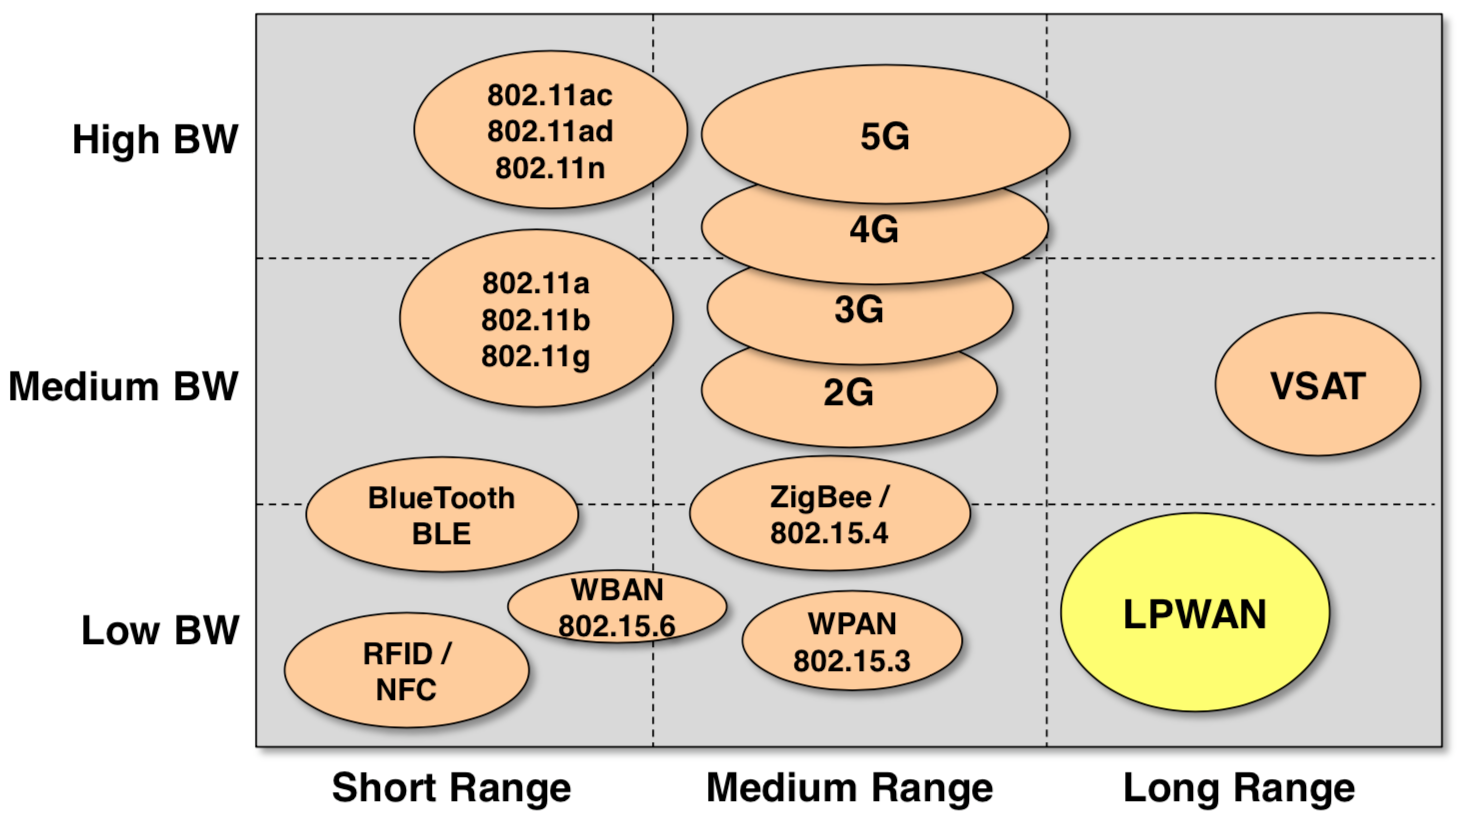
\includegraphics[width=\textwidth]{confronto.png}
\caption[Confronto tra differenti tecnologie wireless]{Confronto tra differenti tecnologie wireless}\label{fig:prima}
\end{center}
\end{figure}
Ad oggi non esiste una risposta unica alle pi\`u svariate esigenze applicative. La scelta di una tecnologia ottimale a garantire una buona qualit\`a di servizio deriva da una profonda analisi dei requisiti dell'applicazione ma soprattutto del contesto ambientale in cui si opera. 
Per poter fare un confronto tra le diverse tecnologie wireless, al fine di poter stabilire quale si adatta meglio al contesto applicativo preso in esame, \`e possibile analizzare alcuni parametri. 
I parametri da analizzare per il confronto sono:  link budget, sensitivit\`a del ricevitore, rapporto tra modulazione e sensitivit\`a e tecniche di modulazione.

\section{Link Budget}
Il link budget, o bilancio di collegamento, indica la relazione formale che stabilisce il bilancio di potenza di un sistema di telecomunicazione tra la potenza ricevuta dal ricevitore in funzione di quella emessa dall'apparato trasmittente e che include tutti i fattori di amplificazione e dissipativi lungo il canale di comunicazione \cite{K1}. 

\begin{equation*} LB = P_{rx} - RS \end{equation*}

Dove:
\begin{itemize}                       
\item LB = Link Budget espresso in dBm 
\item $ P_{rx}$ = Potenza di segnale ricevuta espressa in dBm 
\item RS = Receiver Sensitivity espressa in dBm
\end{itemize}

\section{Sensitivit\`a del ricevitore}
Un altro importante fattore che determina le performance delle trasmissioni \`e la soglia di sensitivit\`a del ricevitore radio. 
La sensitivit\`a di un ricevitore radio \`e la quantit\`a minima di segnale utile richiesto per poter decifrare un'informazione ad uno specifico error rate in relazione al rapporto tra segnale e rumore (SNR). 
In altre parole quanto pi\`u l'antenna ricevente \`e sensibile alla ricezione del segnale tanto meno sar\`a l'energia necessaria per demodulare il segnale in ricezione. 
Ad esempio se si considera un'antenna che pu\`o trasmettere ad una potenza di +15 dBm e il segnale ha una perdita di potenza di -140 dBm il segnale ricevuto dal dispositivo sar\`a di -125 dBm. 
La soglia di sensitivit\`a \`e un parametro molto importante per il confronto delle varie tecnologie wireless.
In generale \`e possibile affermare che la comunicazione tra un sender ed un receiver \`e possibile se la sensitivit\`a del ricevitore $S_{Rx}$ \`e minore o uguale alla potenza di segnale ricevuta $P_{Rx}$.  


\begin{equation*} S_{Rx} <= P_{Rx} \end{equation*}

Bisogna considerare che per le trasmissione a lungo raggio, il path loss ovvero la perdita di segnale nello spazio aperto, \`e il fattore dominante che riduce notevolmente la potenza di segnale ricevuta $P_{Rx}$.
La potenza di segnale ricevuta $P_{Rx}$ \`e determinata da una serie di fattori, ed calcolata con la seguente formula :

\begin{equation*} P_{Rx}= P_{Tx} + G_{Tx} - L_{Tx}- L_{Fs} - L_{M} + G_{Rx} - L_{Rx} \end{equation*}

Dove:
\begin{itemize} 
\item $P_{Rx}$ = Potenza ricevuta(dBm)
\item $P_{Tx}$ = Potenza trasmessa (dBm)
\item $G_{Tx}$ = Guadagno antenna trasmettitore (dBi)
\item $L_{Tx}$ = Perdita segnale trasmettitore (dispersione energetica dei connettori)
\item $L_{Fs}$ = Perdita segnale in spazio aperto (dB)
\item $L_{M}$ = Perdita segnale causato da diversi fattori (dB) (multipath fading, shadowing, scattering)
\item $ G_{Rx}$ = Guadagno antenna ricevitore
\item $ L_{Rx}$ = Perdita segnale ricevitore (dispersione energetica dei connettori)
\end{itemize}

\section{Capacit\`a del canale}
La capacit\`a di canale viene definita come :

\itshape
Il pi\`u piccolo ``limite superiore'' alla quantit\`a di informazione che pu\`o essere trasmessa in maniera affidabile su un canale. Secondo il teorema della codifica del canale, la capacit\`a di un certo canale \`e il massimo tasso di trasferimento di dati che pu\`o fornire il canale per un dato livello di rapporto segnale/rumore, con un tasso di errore piccolo a piacere \cite{K1}.

\normalshape
A partire da questa definizione \`e possibile fare due considerazioni per capire se la scelta di una tecnologia wireless \`e adeguata per il contesto applicativo analizzato.  
La prima considerazione \`e se il canale trasmissivo fornisce una adeguata capacit\`a di banda che si traduce in quantit\`a di bit rate sufficiente al trasporto delle informazioni necessarie all'applicazione. 
La seconda considerazione riguarda la presenza di rumore sul canale. 
In ambienti industriali, cos\`i come in presenza di porti navali vi \`e una forte presenza di rumore che genera disturbo alle trasmissioni. In questo caso \`e necessario adottare soluzioni che prediligono la robustezza del segnale rispetto ad un maggiore bit rate.
La capacit\`a del canale si ricava in questo modo:
\begin{equation*} C = 2BW \end{equation*}
Dove BW\`e la bandwidth. Questa formula si applica solo in presenza di un segnale ideale sprovvisto di codifica e di rumore.
Quando il segnale \`e libero da rumore ma \`e presente la codifica allora si applica la seguente formula :
\begin{equation*} C =2BWlog_2M \end{equation*}
dove M rappresenta il numero di livelli di codifica.
Per rappresentare la capacit\`a del canale in presenza di codifica e rumore si usa il modello del teorema di Shannon-Hartley:
\begin{equation*} C=BWlog_2(1 + \tfrac{S}{N}) \end{equation*}
Dove S rappresenta il segnale ed N il rumore ovvero il rapporto tra segnale e rumore (SNR).
Un aspetto critico imposto dal modello di Shannon-Hartley \`e dato da $\tfrac{E_b}{N_0}$, ovvero il rapporto che esiste tra la quantit\`a di energia necessaria per rappresentare un bit ed il livello di rumore della densit\`a spettrale che di fatto indica la misura di SNR.
L'efficienza spettrale $\eta$ indica il quantitativo di dati che \`e possibile trasmettere su una determinata bandwidth :
\begin{equation*} \eta= \frac{C}{BW} \end{equation*}

Considerando che C \`e il massimo data rate del canale e BW \`e un valore fisso, l'utilizzo di una buona modulazione diventa un parametro fondamentale per massimizzare $\eta$ che si traduce nel massimizzare il throughput dei dati. 
Pertanto, quando $\eta$ aumenta allora anche $\tfrac{E_b}{N_0}$ deve aumentare, ovvero \`e necessaria una potenza energetica per rappresentare un bit, che corrisponde ad un  maggior consumo energetico delle batterie. 
Quanto pi\`u energia serve per rappresentare un bit tanto inferiore sar\`a la vita delle batterie. 
Inoltre per fronteggiare il problema delle interferenze e degli ostacoli si pu\`o aumentare il time on air di trasmissione del segnale attraverso l'utilizzo di una modulazione lenta. 

\section{Tecniche di trasmissione dei dati}
I dati quando vengono trasmessi mediante radiofrequenze si propagano tutti alla velocit\`a della luce. Quello che differisce tra le varie tecnologie wireless \`e il throughput, ovvero la quantit\`a di dati che pu\`o essere trasferita in unit\`a di tempo e viene misurato in Bit per Secondo (bps).
Per poter trasferire una maggiore quantit\`a di dati a parit\`a di tempo \`e necessario che l'ampiezza di banda in trasmissione sia sufficientemente capiente al trasporto dei dati.
Per poter ottenere canali di comunicazione ad elevato bit rate \`e necessario disporre di un canale di comunicazione con una banda abbastanza ampia. 
Solitamente si parla di broadband per velocit\`a superiori a 1 Mbps, mentre al di sotto di questa velocit\`a si parla di narrow band. 
Per le applicazioni che richiedono un alto data rate bisogna utilizzare connessioni broadband che vanno accompagnate con elevate frequenze. 
Per le applicazioni che richiedono una copertura di segnale a lungo raggio, bisogna usare trasmissioni narrow band in quanto queste concentrano l'energia in una porzione di spettro pi\`u piccola risultando meno suscettibili alla presenza di rumore. 
\\
\\
\\
\\
\\
\\
\begin{figure}[h!]
\begin{center}

\graphicspath{https://it.overleaf.com/project/5bb23fa816bccf0dedc574b9/file/5bd89848833ef87f15059f1d}
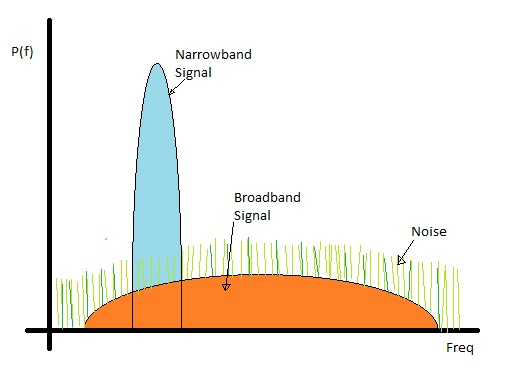
\includegraphics[width=\textwidth]{Broadband-vs-Narrowband.jpg}
\caption{Segnali Narrowband e Broadband}
\label{fig:seconda}
%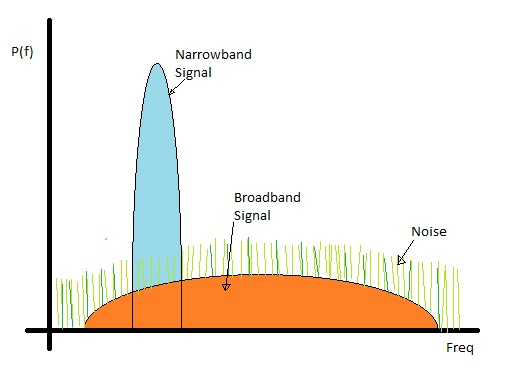
\includegraphics[scale=0.5]{Broadband-vs-Narrowband.jpg}

%\caption[legenda elenco figure]{Segnali Narrowband e %Broadband}\label{fig:seconda}
\end{center}
\end{figure}

\par\bigskip 
\noindent
Le trasmissioni broadband occupano molta bandwidth rispetto alle trasmissioni narrowband, ma la potenza di trasmissione \`e inferiore.
La tabella \ref{tab:uno} riepiloga le principali differenze tra i due tipi di trasmissione.


\begin{table}[h]                        %ambiente tabella
                                        %(serve per avere la legenda)
\begin{center}                          %centra nella pagina la tabella
\begin{tabular}{r|c|c}                  %tre colonne con righe verticali
                                        %   prodotte con |
                           %inserisce due righe orizzontali
$Specifiche$ & $Broadband$ & $Narrowband$\\           %& separa le colonne e con
\hline\hline                                   %inserisce una riga orizzontale
$Efficienza spettrale$ & $Bassa$ & $Molto\ alta$\\           %  \\ va a capo
\hline                                  %inserisce una riga orizzontale
$Throughput$ & $Alto$ & $Basso$\\
\hline                                  %inserisce una riga orizzontale
$Distanza copertura$ & $Bassa$ & $Alta$\\
\hline                                  %inserisce una riga orizzontale
$Penetrazione ostacoli$ & $Bassa$ & $$Alta$$\\
\hline                                  %inserisce una riga orizzontale
$Lunghezza codici preambolo$ & $Lungo$ & $Corto$\\
\hline \hline                           %inserisce due righe orizzontali
\end{tabular}
\caption[Ripilogo caratteristiche trasmissioni Broadband e Narrowband]{Ripilogo caratteristiche trasmissioni Broadband e Narrowband}\label{tab:uno}
\end{center}
\end{table}


Un modo per ovviare al problema di mantenere un buon compromesso tra energia impiegata per codificare il segnale e la presenza di rumore che distorce l'informazione \`e quello di usare trasmissioni narrowband con una dimensione del canale molto stretta. 
Dato che il rumore si disperde su tutto lo spettro, le trasmissioni narrowband hanno un pi\`u basso livello di rumore su singolo canale. Quando si usano canali narrowband il canale non \`e molto disturbato dalle interferenze dei canali vicini, ma se l'interferenza si manifesta sullo stesso canale allora la trasmissione viene persa. 
Per questo motivo esse si adattano meglio alle trasmissioni a lungo raggio che sono caratterizzate da una forte attenuazione del segnale.
Per poter ottenere trasmissioni in broadband bisogna usare tecniche di modulazione in grado di elaborare il segnale di base ed a parit\`a di ampiezza questo viene disperso su una porzione di spettro pi\`u ampia. Questa tecnica \`e conosciuta come spread spectrum.
Nelle trasmissioni spread spectrum il segnale in banda base viene trasmesso su una banda di frequenze pi\`u ampia di quella effettivamente necessaria alla trasmissione dell'informazione contenuta nel segnale originario stesso, in contrapposizione alle trasmissioni narrowband in cui la trasmissione non eccede mai la reale capacit\`a del canale trasmissivo.
Il segnale in banda base viene inviato ad un codificatore di canale che produce un segnale analogico di ampiezza di banda relativamente limitata centrata su una determinata frequenza. Il segnale viene modulato usando una sequenza di cifre chiamato codice o sequenza di dispersione. In generale il codice di dispersione viene prodotto da un generatore di pseudo rumore o numeri pseudo casuali. L'effetto di questa modulazione \`e quello di aumentare sensibilmente l'ampiezza di banda (dispersione dello spettro) del segnale da trasmettere. Il ricevente, allo stesso modo, deve conoscere la stessa sequenza di cifre. Il segnale viene inviato ad un decoder di canale che recupera i dati in esso contenuti. 

I vantaggi principali ottenuti usando una tecnica spread spectrum sono:
\begin{itemize}                       
\item Pi\`u stazioni radio possono trasmettere contemporaneamente usando la stessa ampiezza di banda con interferenza reciproca minima migliorando rapporto segnale/rumore.
\item Riduzione incidenza delle interferenze.
\item Nascondere e crittografare i segnali.  
\end{itemize}


\begin{figure}[h]                      
\begin{center} 

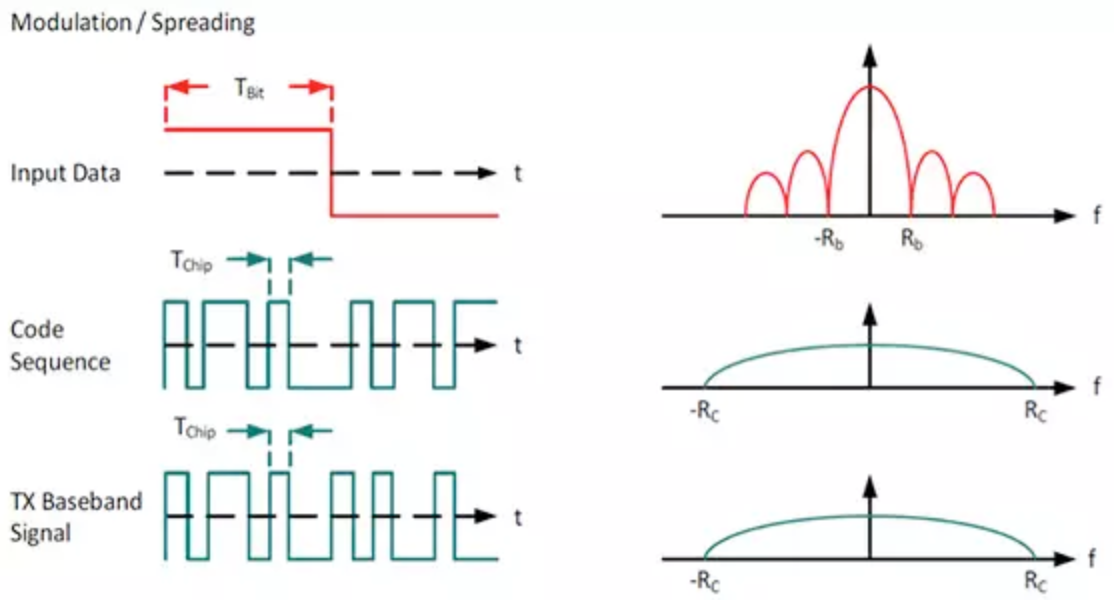
\includegraphics[width=\textwidth]{spreading_factor.png}
\caption[Un sistema di divisione di spettro]{Un sistema di divisione di spettro}\label{fig:prima}
\end{center}
\end{figure}
Esistono diverse tecniche di dispersione dello spettro. Tra le pi\`u comuni troviamo: 
FHSS (Frequency Hopping Spread Spectrum) in cui il segnale viene trasmesso su una serie di frequenze pseudocasuali, saltando da una frequenza all'altra a intervalli regolari. Questa tecnica \`e usata dalla tecnologia Bluetooth.
DSSS (Direct Sequence Spread Spectrum) che utilizza un codice di dispersione per permettere a ciascun bit del segnale originario di essere rappresentato da pi\`u bit del segnale trasmesso. Una sequenza di bit di codice lunga per ogni bit di segnale produce un ampio guadagno elaborato paragonabile all'aumento di potenza in db. Questa tecnica \`e impiegata negli standard 802.11-b ed 802.11-g .
CSS (Chirp Spread Spectrum) utilizzato da LoRa \`e una  tecnica di modulazione in frequenza lineare a larga banda (chirp) degli impulsi da codificare. Un chirp \`e un segnale sinusoidale la cui frequenza aumenta o diminuisce nel tempo.
Lo svantaggio nell'utilizzo di tecniche spread spectrum come modulazione \`e che il ricevitore deve fare pi\`u lavoro per decodificare l'informazione da un segnale che si confonde con il rumore di fondo. Inoltre disperdere un segnale narrowband su una banda pi\`u ampia rappresenta un modo meno efficiente di utilizzo dello spettro. Questo problema viene per\`o risolto attraverso l'uso di pi\`u sequenze tra loro ortogonali. Dato che pi\`u dispositivi possono usare canali diversi o sequenze ortogonali, si riesce ad ottenere un incremento di capacit\`a della rete. 

\chapter{LR-WPAN e 6LowPAN}
Pima dell'avvento delle tecnologie LPWAN l'unico standard di riferimento per le WSN (Wireless Sernsor Network) \`e stato LR-PWAN, ratificato dall'IEEE attraverso il protocollo 802.15.4 che definisce i livelli PHY e MAC. 
Al fine di favorire l'interoperabilit\`a, lo stesso ente di standardizzazione, ha sviluppato il protocollo 6LowPan che implementa il livello network compliance allo standard 802.15.4.

\section{Standard IEEE 802.15.4}
LR-WPAN (Low Rate - Wireless Personal Area Network) \`e una tecnologia pensata per trasmettere piccole informazioni su brevi distanze con basso data rate. 
A differenza delle WLAN (reti locali senza fili), i collegamenti effettuati tramite WPAN coinvolgono poco o nessuna infrastruttura. Questa caratteristica permette soluzioni piccole, economiche ed energeticamente efficienti da attuare per una vasta gamma di dispositivi.
Lo scopo dello standard IEEE 802.15.4 \`e quello di definire il livello fisico ed il livello MAC per la connettivit\`a wireless a bassa velocit\`a di trasmissione dati. 
Le WPAN permettono di integrare dispositivi fissi e mobili, che possono essere alimentati con o senza batteria. Qualora fossero alimentati a batteria il consumo \`e molto limitato grazie ai requisiti molto bassi di computazione. Tipicamente il raggio operativo dei dispositivi \`e di 10 mt e viene identificato come POS (Personal Operating Space). 
E\` possibile prevedere, in base ai requisiti dell'applicazione, un raggio di copertura pi\`u ampio a discapito di un data rate inferiore come accettabile compromesso. 		 	 
Lo standard definisce due tipi di dispositivi, i Full Function Device (FFD) con funzionalit\`a complete e Reduced Function Device (RFD) con funzioni limitate. I primi implementano all'interno del loro firmware tutto lo stack e possono assumere i ruoli sia di coordinatore della rete che di router per l'instradamento dei pacchetti tra segmenti di rete differenti.
Ogni rete deve includere almeno un FFD che agisce come coordinatore della WPAN che pu\`o inoltre operare come normale device. Gli RFD svolgono invece operazioni molto semplici, non devono elaborare o spedire grandi quantit\`a di dati e possono rimanere inattivi quando non hanno necessit\`a di comunicare. Un FFD pu\`o comunicare sia con altri FFD che con gli RFD, mentre questi ultimi possono comunicare solo con altri RFD. In questo modo \`e possibile costruire una WPAN quando almeno 2 dispositivi comunicano all'interno dello stesso POS, utilizzando lo stesso canale fisico. 


\section{Topologie LR-WPAN}
Lo standard 802.15.4 supporta la creazione di tre topologie di reti: a stella, ad albero e mesh.
In una topologia a stella la rete \`e controllata da un singolo dispositivo chiamato coordinatore. 
Solo i dispositivi FFD possono assumere il ruolo di coordinatore, in quanto implementano a bordo del proprio firmware tutto lo stack. 
Il coordinatore \`e responsabile di inizializzare la rete stessa e di coordinare la comunicazione tra i dispositivi nella rete. Tutti gli altri nodi, conosciuti come end-devices, comunicano solo con il coordinatore.
Nella topologia ad albero e a mesh il coordinatore inizializza la rete e definisce i parametri necessari alla comunicazione ma l'instradamento per poter comunicare con altre reti avviene solo tramite i routers. Nella topologia ad albero, i routers, muovono dati e controllano la rete attraverso una strategia di routing gerarchico. Ogni router pu\`o essere rappresentativo di un cluster di nodi, pertanto nella topologia ad albero \`e possibile supportare fino a 255 cluster composti da 254 nodi ciascuno per un totale di oltre 64 mila nodi. Un caratteristica interessante della topologia ad albero \`e che un nodo potrebbe decidere di passare da un segmento di rete ad un altro semplicemente facendo facendo uno switch del canale radio su cui trasmette. Questa caratteristica \`e permessa in quanto vale il meccanismo di accesso al canale condiviso sul principio del ``chi parla quando''. 
La topologia ad albero potrebbe implementare una comunicazione beacons oriented come definito nello standard 802.15.4 . 
La rete mesh permette una comunicazione P2P . I routers nella mesh network non emettono beacons regolari come definito nello standards 802.15.4, in quanto questa specifica descrive solo reti intra PAN, cio\`e le reti in cui cominciano le comunicazioni e terminano nella rete stessa. Le reti mesh permettono una grande scalabilit\`a e disponibilit\`a di servizio , in quanto permettono di estendere la rete aggiungendo nuovi nodi router i quali possono instradare le comunicazioni sfruttando path multipli. Nelle reti mesh viene impiegato il protocollo AODV per la gestione del routing. Il protocollo AODV (Ad-hoc On-demand Distance Vector) \`e un protocollo dinamico di tipo reattivo che fa uso di tabelle di routing locali ai nodi per poter instradare i pacchetti verso altri nodi. All'interno delle reti mesh i nodi sono statici e per questo si differenziano dalle reti Ad-hoc. Il protocollo AODV funziona bene nelle reti di sensori in quanto le tabelle di instradamento non vengono aggiornate molto frequentemente, salvo quando un nodo fallisce.
\begin{figure}[h]                      
\begin{center} 
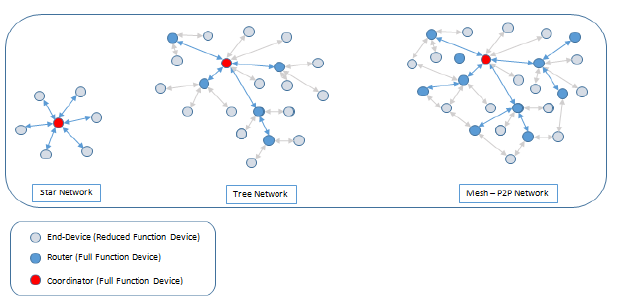
\includegraphics[width=\textwidth]{EEE-802154-network-topologies-with-device-types.png}
\caption[Topologie reti LR-WPAN]{Topologie reti LR-WPAN}\label{fig:nona}
\end{center}
\end{figure}
\\
\\
\\
\\
\\
\\

\section{6LowPAN}
La specifica dello standard IEEE 802.15.4 definisce solo i livelli PHY e MAC dello stack e non fornisce alcuna indicazione sui layers superiori. 
Le tecnologie compliance a questo standard, come ZigBee o WirelessHart, implementano i layers superiori sulla base delle proprie specifiche per ottenere lo stack completo.  
Il limite di questo tipo di approccio \`e che due device sono conformi alle specifiche dello standard, ma afferiscono a tecnologie differenti, non sono in grado di comunicare tra loro in quanto i layers superiori a quello fisico e mac sono completamente diversi. 
Nell'ambito dell'IoT questo potrebbe rappresentare un grosso limite, pertanto, per favorire l'interoperabilit\`a tra tecnologie eterogenee \`e stato pensato di sviluppare uno standard per il livello rete che favorisca lo scambio di dati. 
Nelle reti LAN tradizionali il livello rete \`e gestito dal protocollo IP. 
Nel protocollo IP la lunghezza degli indirizzi che si possono assegnare ad una interfaccia di rete \`e di 32 bit. Il proliferare di numero di hosts connessi alla rete ha messo in crisi lo spazio di indirizzamento possibile del protocollo IP. 
Per sopperire a questa problematica, a fine anni 90 venne definito tramite RFC 2460, il protocollo IPv6. La nuova versione del protocollo IP prevede l'utilizzo di indirizzi lunghi 128 bit, consentendo uno spazio di indirizzamento molto pi\`u ampio.
Con l'esplosione dell'IoT il numero di dispositivi che necessitano di connettivit\`a crescer\`a in modo esponenziale. Considerato che gli indirizzi IPv4 sono in via di esaurimento, sarebbe impossibile coniugare l'esigenza di connettivit\`a dei dispositivi con la scarsa disponibilit\`a di risorse. Il protocollo IPv6 offre un ampio spazio di indirizzamento e sarebbe sufficiente a garantire il deploy su larga scala di un elevato numero di nodi.
Considerati questi aspetti, IETF ha proposto uno standard basato su protocollo IPv6 che potesse adattarsi al contesto delle reti LR-WPAN. Nel 2007 venne definito tramite RFC 4944 lo standard 6LowPAN (IPv6 over Low-rate WPAN). 
L'obiettivo primario di questo standard \`e quello di definire un network layer comune per tutte le tecnologie che si basano sullo standard IEEE 802.15.4.
Lo standard 6LowPAN va anche incontro al problema di interoperabilit\`a delle reti LPWAN. 
Tuttavia, in ambito LPWAN, il protocollo 6LowPAN ha un'accezione diversa a causa di alcuni aspetti. Innanzi tutto bisogna considerare che essendoci una pletora di tecnologie differenti, ognuna di esse utilizza un proprio standard per l'implementazione del livello PHY e MAC. 
Le reti LR-WPAN, invece, sono definite dallo standard IEEE 802.15.4 pertanto \`e pi\`u naturale costruire uno standard per l'implementazione del livello rete.
In secondo luogo bisogna considerare che la maggior parte delle reti LPWAN ha una topologia a stella in cui la base station comunica con gli end-device tramite una specifica tecnologia wireless. La base station \`e connessa ai sistemi di back-end tramite protocollo IPv4. In questo scenario ha meno senso dotare gli end-device di uno stack completo che comprenda il livello rete in quanto aumenterebbe la complessit\`a dei dispositivi e farebbe aumentare i costi di produzione.   

\section{6LowPAN : Caratteristiche tecniche}
Lo standard 6LowPAN permette di usare il protocollo IPv6 su sistemi embedded.
Sebbene questo aspetto permette il deploy su larga scala di una grande vastit\`a di dispositivi, non \`e esule da criticit\`a. Il primo fattore critico da considerare \`e che originariamente il protcollo IPv6 non venne concepito per poter essere implementato su tecnologie con scarse risorse computazionali, di consegueza deve essere ridimensionato e alleggerito.
In secondo luogo bisogna considerare che il livello MAC dello standard 802.15.4 \`e diverso dal livello MAC degli standard delle reti LAN.
La dimensione del payload supportato dal layer MAC in IPv6 \`e molto pi\`u grande di quello definito dallo standard IEEE 802.15.4. 
Per integrare il protocollo IPv6 sul livello mac, il working group 6LowPAN ha progettato lo stack interponendo tra il livello MAC ed il livello rete un livello chiamato adaptation layer che ha lo scopo di gestire la compressione dell'header, la frammentazione, il riassemblamento e la gestione del routing nella topologia mesh.	
\begin{figure}[h]                      
\begin{center} 
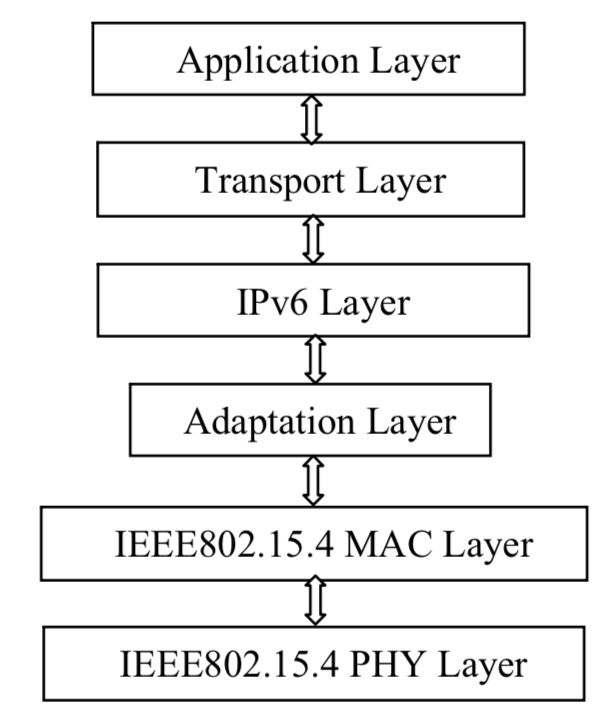
\includegraphics[width=\textwidth,height=110mm]{6lowpan_stack.png}
\caption[6LowPan stack]{6LowPan stack}\label{fig:decima}
\end{center}
\end{figure}
L'utilizzo di uno standard che definisce il layer di rete favorisce non l'interoperabilit\`a con altre tecnologie ma anche l'interazione con i layer superiori. Questo aspetto da origine a diversi vantaggi. 	
Il protocollo IPv6 per quanto possa essere considerato una tecnologia robusta, ancora oggi non \`e ampiamente utilizzato. Le applicazioni che si basano su protocollo IP sono lo standard de facto dei servizi in circolazione. 
L'implementazione del protocollo IPv6 sui sistemi embedded potrebbe favorire la sua sua diffusione.		
Il problema della scarsa disponibilit\`a di indirizzi IPv4 \`e una tematica che viene discussa da diversi anni. Il protocollo IPv6 risolve questo problema offrendo uno spazio di indirizzamento molto ampio che si coniuga con le esigenze di deploy su larga scala dei devices.	
Tra i punti di forza di IPv6 c'\`e la peculiarit\`a che un host \`e in grado di auto assegnare un indirizzo di rete ad una interfaccia fisica che sia globalmente riconosciuto. 
In questo modo si semplificano le architetture di rete in quanto non \`e necessaria la presenza dei NAT (Network Address Translation) e quindi si evita di dover ricorrere all'uso di indirizzi IP privati.   			
Lo standard IEEE 802.15.4 supporta tre topologie di rete, ma in nessuna di queste \`e previsto un accesso diretto alla rete internet da parte dei dispositivi. 
Senza il layer di rete, sarebbe impossibile per un device presente in una rete LR-WPAN interagire con un device collocato su un'altra rete. Tramite 6LowPan, invece, \`e possibile far scambiare i dati a nodi collocati su reti diverse.	

La dimensione massima del frame definito dallo standard IEEE 802.15.4 \`e di 127 byte, la dimensiona massima 
Un frame a livello MAC dello standard IEEE 802.15.4 pu\`o avere dimensione massima di 127 byte, di cui 25 byte vengono destinati all'header ed i restanti 102 byte sono riservati al payload.
Un pacchetto IPv6 pu\`o assumere dimensioni massime di 1280 byte, pertanto non \`e possibile incapsulare un pacchetto IPv6 in un frame 802.15.4. 
L'incapsulamento avviene tramite frammentazione, ovvero i pacchetti del layer IPv6 vengono spezzati in pi\`u pacchetti di dimensioni pi\`u piccole che possono essere contenuti in un frame. 
Al contrario quando un frame deve essere trasportato dal livello MAC verso il livello rete deve essere riassemblato per ricostruire il pacchetto originale.
Le operazioni di frammentazione e riassemblamento vengono svolte dall' adaptation layer.
Tra le features pi\`u interessanti di 6LowPAN c'\`e la possibilit\`a di utilizzare l'assegnamento dinamico degli indirizzi brevi a 16 bit. Usando questi indirizzi \`e possibile implementare il routing gerarchico. 	
Le reti LR-WPAN, essendo composte da dispositivi che dispongono di scarse risorse computazionali, non possono disporre degli stessi servizi di una rete LAN tradizionale. 
IPv6 va nella direzione della semplificazione dell'infrastruttura di rete grazie alla feature chiamata stateless address auto configuration che permette di auto assegnare un indirizzo ad un host senza ricorrere ad servizio di DHCP. In uno scenario applicativo in cui viene fatto il deploy di migliaia di nodi, la possibilit\`a che ogni dispositivo sia in grado di auto assegnarsi un indirizzo semplifica notevolmente la gestione riducendo i costi di messa in produzione.    
Il vantaggio pi\`u grande che offre l'adozione di 6LowPAN \`e che i protocolli del livello applicazione possono essere utilizzati senza dover essere adattati alle LR-WPAN. 
Anche le socket possono essere usate senza subire nessuna modifica.
La messa in produzione di un'infrastruttura di rete implica che gli hosts vengano monitorati al fine di garantire un buon livello di servizio. 
Quando un nodo della rete, un apparato o una singola componente subisce un guasto \`e necessario che gli operatori che amministrano il servizio intervengano per gestire il guasto.  
Il protocollo SNMP (Simple Network Management Protocol) \`e stato sviluppato per poter raccogliere in tempo reale dati sullo stato di salute degli hosts. 
Nell'ambito IoT in cui le reti possono essere composte da migliaia di nodi \`e fondamentale avere un servizio che permetta il monitoraggio di tutte le componenti, soprattutto in contesti in cui si opera in aree remote in cui non \`e facile intervenire tempestivamente \cite{K19}.




\chapter{LPWAN}
I requisiti fondamentali che hanno guidato la progettazione delle reti LPWAN sono : trasmissioni a lungo raggio nell'ordine dei chilometri, basso data rate inferiore a 5000 bits per secondo, basso consumo energetico da parte dei dispositivi che si riflette sulla durata delle batterie dai 5 ai 10 anni, capacit\`a di gestire le connessioni di migliaia di dispositivi contemporaneamente. \cite{K2}
Nei paragrafi seguenti verranno approfonditi i seguenti aspetti delle reti LPWAN:
\begin{itemize}                       
\item Trasmissione a lungo raggio 
 \item Efficienza energetica
\item Basso costo di produzione dei dispositivi
\item Scalabilit\`a
\item Quality of Service
\end{itemize}

\section{Trasmissione a lungo raggio}
Le trasmissioni radio possono essere a corto raggio quando operano su distanze nell'ordine dei metri oppure a lungo raggio quando si arriva sull'ordine dei chilometri.
I parametri che determinano la distanza della copertura di segnale sono: la potenza trasmissiva, la banda di frequenza, la tecnica di modulazione del segnale, trasmissione narrow band  o spread spectrum. 

Molte tecnologie wireless LPWAN utilizzano bande di frequenze inferiori ad 1 GHz, conosciute come frequenze Sub-Ghz. 
Questo spettro di frequenze offre trasmissioni robuste e affidabili con un basso link budget. 
La frequenza dei 2.4 GHZ risente dei problemi di attenuazione del segnale dopo brevi distanze, del multipath fading causato dagli ostacoli, e dalla scarsa capacit\`a di oltrepassare gli ostacoli. 
Inoltre la banda di frequenza dei 2.4 GHz \`e congestionata dalla presenza di innumerevoli tecnologie wireless quali Wi-Fi, telefoni cordless, Bluetooth, Zigbee che possono creare livelli di interferenza. 
Nonostante questi aspetti alcune tecnologie LPWAN utilizzano la banda dei 2.4 GHz. Tuttavia l'utilizzo di bande Sub-GHz offre nettamente performance migliori sulle lunghe distanze.
Per le tecnologie LPWAN il link budget si attesta sui 150 $\pm$ 10dBm che garantisce copertura nel raggio di qualche chilometro in ambito cittadino e fino a 10 chilometri in ambito rurale. 
Per permettere al ricevitore di decodificare informazioni anche in presenza di forte attenuazione del segnale, il livello fisico dello stack deve effettuare un compromesso tra bit rate e rallentamento della velocit\`a di modulazione cos\`i da disporre di pi\`u energia per ogni bit inviato. 
Le tecnologie LPWAN hanno una soglia di sensitivit\`a che raggiunge i -130 dBm.
Le trasmissioni narrow band decodificano il segnale trasmesso su una porzione di spettro molto stretta.
Assegnando ad ogni canale una banda stretta, tipicamente meno di 25 MHz, \`e possibile ottenere molti canali che condividono lo stesso spettro. 
Il vantaggio ottenuto \`e che il livello di rumore su singolo canale \`e minimo, ed inoltre il ricevitore non deve svolgere alcun compito aggiuntivo per decodificare l'informazione, rendendolo semplice e poco costoso il design.  
NB-IoT and Weightless-P sono esempi di tecnologie che usano la tecnica narrow band, mentre esistono altre tecnologie che utilizzano canali ancora pi\`u stretti intorno ai 100Hz e vengono identificate come Ultra Narrow Band (UNB). 
In questo modo si riduce ulteriormente il rumore ed \`e possibile incrementare il numero di dispositivi in grado di trasmettere sulla stessa banda. Sebbene il data rate effettivo per singolo dispositivo diminuisce, aumenta il tempo in cui il ricevitore radio deve essere acceso. Il basso data rate in combinazione con la regolamentazione per l'accesso condiviso allo spettro di frequenza pu\`o avere ripercussioni sulla dimensione massima dei pacchetti e sulla frequenza di invio degli stessi, limitando i possibili casi applicativi.
Alcuni esempi di tecnologie che usando UNB sono SigFox, Weightless-N, Telensa.
Le tecniche di trasmissione spread spectrum aumentano l'occupazione di banda del segnale a parit\`a di energia impiegata (ampiezza fissa).  In questo modo, senza variare il contenuto energetico (elemento cruciale nelle LPWAN), \`e possibile migliorare il rapporto tra segnale/rumore eliminando il maggior numero di interferenze possibili. 
Questo consente l'utilizzo contemporaneo della stessa gamma di frequenze a pi\`u dispositivi ottenendo un miglioramento nella gestione dello spettro. 
Uno scopo secondario della tecnica spread spectrum, utilizzato soprattutto in ambito militare, \`e quello di minimizzare il segnale radio trasmesso abbassando la potenza specifica e portandolo a confondersi con il rumore radio di fondo in modo da sfuggire al rilevamento da parte delle stazioni di intercettazione radio. \cite{K2}

\section{Efficienza energetica}
L'efficienza energetica \`e un aspetto cruciale per il funzionamento delle applicazioni IoT.
I dispositivi una volta configurati e posizionati devono svolgere il loro compito per il maggior tempo possibile senza intervento umano. 
Questo aspetto \`e fondamentale se si vogliono contenere i costi di gestione del servizio. 
La maggior parte dei dispositivi \`e alimentato a batteria, pertanto la frequenza di manutenzione per la sostituzione o ricarica deve essere ridotta al minimo.
Si stima che per mantenere i costi di gestione bassi, \`e necessario che la vita delle batterie debba durare dai 5 ai 10 anni. 
Per poter avere una maggiore efficienza energetica \`e possibile adottare diverse misure a livello di infrastruttura, complessit\`a, frequenza di invio dei dati e politiche di accesso al mezzo trasmissivo.
La topologia della rete ha influenza sul consumo energetico.
Le reti mesh vengono impiegate  per estendere la copertura di segnale delle reti wireless che usano tecnologie con trasmissioni a breve o medio raggio. Il consumo energetico dei dispositivi \`e maggiore rispetto ad una topologia a stella. 
Il motivo deriva dal fatto che mentre nelle topologie a stella c'\`e un solo nodo in grado di instradare il traffico, nelle reti mesh possono esserci pi\`u dispositivi con il ruolo di router.
I nodi con il ruolo di router devono essere sempre accesi ed in ascolto del canale. 
In alcuni casi questi nodi potrebbero essere congestionati, con un ulteriore aggravio del consumo energetico.  
Inoltre l'uso di una topologia a stella per la copertura di una vasta area geografica implica una minore densit\`a di dispositivi da utilizzare, che fa abbassare ulteriormente i costi di gestione ed il livello di interferenza. 

Per poter ottenere un maggiore risparmio energetico \`e possibile spegnere il ricevitore radio quando non c'\`e necessit\`a di trasmissione o ricezione. 
Se gli end-device non dovendo gestire l'instradamento dei pacchetti provenienti dagli altri nodi possono accendere il trasmettitore radio solo quando necessario. 


Il meccanismo del duty cycle \`e subordinato ai requisiti dell'applicazione. 
Il device pu\`o svegliarsi solo all'occorrenza se deve fare delle trasmissioni periodiche in uplink. 
Diverso \`e il caso per le trasmissioni in downlink, in cui sono necessari meccanismi di sincronizzazione tra end-device e gateway se si vuole che il dispositivo si attivi a intervalli schedulati. 
Il modo pi\`u semplice per gestire la ricezione in downlink \`e quello di aprire una finestra in ascolto dopo una comunicazione in uplink.
I dispositivi alimentati da rete elettrica possono essere costantemente in ascolto del canale per ricevere informazioni riducendo anche la latenza delle comunicazioni. 
Il duty cycle non \`e solo una tecnica di risparmio energetico ma anche un vincolo normativo che dipende dalle legislazioni nazionali che regolamentano l'accesso ad uno spettro con banda condivisa evitando che una singola stazione radio monopolizzi il canale.
Per una maggiore efficienza energetica i dispositivi vengono progettati in maniera modulare in modo che \`e possibile spegnere la singola componente quando non utilizzata, quindi applicando il concetto di duty cycle non solo al ricevitore radio ma anche alle altre componenti hardware.

Il livello MAC utilizzato sia nelle reti cellulari che nelle LR-WPAN \`e troppo sofisticato per poter essere impiegato nelle reti LPWAN. 
Il fatto di avere un livello MAC pi\`u sofisticato permette di ottenere dei benefici che potrebbero essere non necessari per il contesto applicativo delle LPWAN. 
Nelle reti cellulari, ad esempio, esistono meccanismi abbastanza sofisticati per garantire a pi\`u stazioni radio di poter comunicare usando la stessa banda di frequenza. 
Alcune tecniche quali TDMA (Time Division Multiple Access) e FDMA (Frequency Division Multiple Access) sono abbastanza complesse e rendono il livello MAC pi\`u pesante. 
Questo si traduce in un grosso dispendio di energia dovuto alle continue sincronizzazioni tra il trasmettitore e ricevitore. 
Le tecniche di accesso multiplo al canale, TDMA e FDMA,  operano rispettivamente nel dominio del tempo e delle frequenze. 
Esse fanno un uso esclusivo del canale di comunicazione, garantendo un'alta qualit\`a del servizio a discapito dei costi di gestione e di implementazione dei dispositivi.
Per mantenere i costi di produzione bassi, molte tecnologie wireless come ad esempio Wi-Fi e Zigbee, usano CSMA/CA (Carrier Sense Multiple Access / Collision Avoidance) per la gestione della contesa del canale da parte di pi\`u stazioni radio. 
L'idea alla base \`e quella di ascoltare il canale e di aspettare per un tempo random prima di effettuare la trasmissione. 
In caso di collisione le stazioni radio coinvolte aumentano il tempo di attesa prima di ritrasmettere. Questo aspetto ha forti ricadute sulle performance globali della rete.
La probabilit\`a di collisione aumenta all'aumentare del numero di stazioni che vogliono trasmettere. Questo aspetto diverge dalle esigenze delle reti LPWAN che devono supportare   
il deploy di migliaia di dispositivi. 
Inoltre per risolvere il problema del terminale nascosto e per garantire un accesso equo a tutte le stazioni radio si usano metodi di Request To Send e Clear To Send (RTS/CTS) che aggiungono molto overhead alle comunicazioni. 
Il problema del terminale nascosto si verifica quando il dispositivo che vuole trasmettere non rileva che il canale \`e impegnato dalla trasmissione di un'altra stazione radio in quanto  quest'ultima \`e fuori dalla sua portata. 
La collisione pu\`o sempre verificarsi al ricevitore, il quale pu\`o trovarsi nel mezzo a pi\`u stazioni e quindi sentirle entrambe, ma queste ultime potrebbero non sentirsi reciprocamente. 
Per semplificare la complessit\`a del livello MAC anzich\`e usare le tecniche precedentemente descritte, molte tecnologie LPWAN usano il protocollo ALOHA che \`e molto pi\`u semplice. 
L'algoritmo del protocollo aloha non prevede l'ascolto del canale, ma semplicemente aspettano un tempo random prima di trasmettere. 
Questo tipo di approccio ha come svantaggio che non \`e esclusa la probabilit\`a di collisione, ma data la sua semplicit\`a permette la realizzazione di dispositivi meno sofisticati.

Per poter ulteriormente ottimizzare il consumo energetico \`e possibile fare in modo che gli end device siano meno complessi possibile, spostando l'intelligenza sui sistemi di backend. Spostare la complessit\`a offre vantaggi sia dal punto di vista della comunicazione che dal punto di vista della computazione.
Per quanto concerne la comunicazione nella topologia a stella la base station \`e un dispositivo pi\`u complesso in quanto in grado di ascoltare pi\`u trasmissioni contemporanee usando diversi canali o segnali ortogonali, ed anche il ruolo di gateway della rete. 
Questo permette all'end-device di inviare dati su un qualsiasi canale disponibile e di poter raggiungere la base station senza usare trasmissioni particolarmente complesse per inizializzare la comunicazione. 
Il ruolo di coordinatore della rete pu\`o essere svolto sia dalla base station, che da un sistema di back-end.
Il coordinatore della rete pu\`o anche adottare meccanismi tali per cui fornisce indicazioni all'end-device su come poter modificare alcuni parametri relativi alle trasmissioni in modo da rendere pi\`u efficiente la comunicazione. 
Se il ruolo di coordinatore \`e svolto dal sistema di back-end, esso pu\`o anche gestire il roaming di un dispositivo da una rete ad un'altra. 
Questo permette di mantenere il design dell'end-device semplice facendo abbassare i costi di produzione.


Dal punto di vista della computazione bisogna analizzare che esiste un trade-off che riguarda il data processing.
Alcune applicazioni hanno come requisito che i dati raccolti dall'end-device vengano inviati molto frequentemente. 
In altre applicazioni, al contrario, i dati potrebbero essere trasmessi anche una sola volta al giorno. 
Dal punti di vista del consumo energetico \`e pi\`u dispendiosa la trasmissione dei dati rispetto all'elaborazione. 
Il trade off del data processing riguarda se i dati vengono inviati raw oppure \`e meglio che vengano sottoposti ad una pre elaborazione. 
Questa valutazione va fatta in base ai requisiti applicativi. Se l'applicazione richiede trasmissioni molto frequenti allora pu\`o avere senso trasmettere i dati senza alcuna elaborazione in modo da non dover gravare ulteriormente sul consumo energetico, mentre nel caso in cui la trasmissioni sono sporadiche \`e meno costoso far fare elaborazioni all'end-device. 
Il vantaggio di far elaborare i dati all'end-device, \`e che vengono inviati meno dati rispetto a quelli raw. L'invio di tanti dati con molta frequenza potrebbe rappresentare il caso pessimo sia dal punto di vista del consumo energetico che delle performance della rete. 
Non essendo possibile fare una stima assoluta, si preferisce in linea di massima mantenere i costi di design dell'end-device molto bassi specialmente in presenza di deploy con un vasto numero di nodi cercando di far svolgere poca computazione al nodo. 
La valutazione pu\`o essere fatta confrontando il costo di trasmissione dei dati rispetto al costo di sostituzione delle batterie. 
Se ad esempio si utilizzano tariffe al consumo sulla base del volume di dati trasmessi allora \`e meglio far fare elaborazioni all'end-device e cercare di trasmettere meno dati possibile. 
Se invece il costo della sostituzione delle batterie \`e molto elevato allora bisogna adottare una strategia conservativa che punti a massimizzare il risparmio energetico. La valutazione della scelta tra l'invio di dati raw o elaborati ricade sul business model dell'applicazione. \cite{K2}

\section{Basso costo di produzione dei dispositivi}
Il grande successo commerciale delle LPWAN \`e dato dalla capacit\`a di connettere un largo numero di end-device pur mantenendo i costi dell'hardware sotto i 5 dollari. \cite{K3}\cite{K4}
Questa accessibilit\`a permette alle LPWAN non solo di coprire un vasto numero di applicazioni possibili, ma di poter competere anche nei domini applicativi in cui si collocano le tecnologie a breve raggio e le reti cellulari. 
LPWAN offre diverse soluzioni per ridurre i costi di investimento (CAPEX) ed i costi di gestione (OPEX) sia per gli utenti finali che per gli operatori di rete. 
L'utilizzo di una topologia a stella, il MAC protocol semplificato, spostare la complessit\`a sui sistemi di back-end sono tutte misure che portano alla riduzione dei costi di produzione degli end-device. 
I tre fattori principali che influiscono sui costi di produzione sono: minore complessit\`a dell'hardware grazie all'uso di transceivers che adottano modulazioni radio semplici, topologia a stella che semplifica il deploy di migliaia di dispositivi senza ricorrere alle reti mesh, utilizzo di bande di frequenza senza licenza che non comporta ulteriori oneri aggiuntivi. 
In questo ultimo caso, qualora venissero usate bande con licenza, \`e possibile che i provider facciano accordi per condividere la banda in concessione ad altri operatori per evitare costi aggiuntivi. 
Questo approccio avviene soprattutto nelle reti cellulari. L'operatore pu\`o scegliere se condividere la banda oppure optare per soluzioni in cui acquista la banda a disponibile ma riduce l'ampiezza di banda di ogni canale in modo da sostenere un numero maggiore di dispositivi connessi. 

\section{Scalabilit\`a}
Uno dei requisiti fondamentali delle LPWAN \`e di poter supportare un elevato numero di nodi connessi anche sull'ordine delle migliaia.
Per quanto riguarda la scalabilit\`a, i dispositivi devono poter lavorare correttamente anche quando aumentano di numero e di densit\`a. 
La scalabilit\`a dell'infrastruttura pu\`o essere ottenuta con diversi metodi.
Per poter far comunicare il pi\`u elevato numero possibile di dispositivi bisogna sfruttare quanto pi\`u possibile la diversit\`a di canali, tempo, spazio e hardware.
Considerando che gli end-device devono essere a basso consumo e poco complessi per loro natura, l'unico modo per massimizzare la diversit\`a \`e di spostare la complessit\`a della trasmissione sulle base station o sui sistemi di back-end. 
Le tecnologie LPWAN impiegano pi\`u canali e pi\`u antenne per gestire in parallelo diverse trasmissioni da e verso gli end-devices. 
Inoltre il fatto di usare pi\`u canali rende le trasmissioni pi\`u affidabili e meno soggette a interferenze. 
Uno dei problemi maggiori che affligge sia le reti cellulari che le reti LR-WPAN \`e la densit\`a di dispositivi presenti su una certa area. 
Maggiore \`e la densit\`a dei dispositivi e maggiore \`e l'interferenza che questi possono avere l'uno con l'altro. 
Nelle reti LPWAN pu\`o anche esserci un problema di sovraccarico della base station. 
Nelle reti cellulari \`e possibile coordinare l'accesso dei dispositivi alle varie celle in maniera efficiente, cosa non possibile per molte reti LPWAN.
Molti sistemi LPWAN ottimizzano non solo la scalabilit\`a in termini di numero di dispositivi connessi ma anche il singolo collegamento con l'end-device. Per poter ottenere prestazioni migliori in termini di efficienza energetica e affidabilit\`a \`e possibile adattare alcuni parametri relativi alla trasmissione, quali ad esempio lo schema di modulazione o il data rate, in maniera dinamica in base al contesto. 
In questo modo, monitorando la qualit\`a del link \`e possibile coordinare gli end-devices presenti all'interno della rete. Questo tipo di soluzione non \`e sempre possibile e i parametri che \`e possibile modificare possono differire tra le varie tecnologie LPWAN. 
Alcuni fattori come l'asimmetria tra trasmissioni in uplink e downlink e il massimo duty-cycle ammissibile possono essere un ostacolo ai meccanismi di adattamento dinamico al contesto. 
Il miglior modo per sfruttare i meccanismi di adaptive data rate si hanno quando \`e la base station a fornire indicazioni all'end-device su come regolare i parametri relativi alla trasmissione, in quanto l'end-device non \`e in grado di fare valutazioni che gli permettono di migliorare la qualit\`a delle trasmissioni. 
Una tecnica possibile, ad esempio, consiste nell'inviare dati ripetutamente su pi\`u canali scelti a caso e di valutare su quale canale la base station riceve la comunicazione migliore. 
Le tecniche di adaptive data rate tipicamente vengono svolte dalle base station o dai sistemi di back-end per mantenere i costi degli end device bassi.
Esiste un trade off tra la scalabilit\`a della rete ed l'uso di end-device a basso costo. 
Molte soluzioni LPWAN pur di mantenere il requisito di basso consumo energetico, limitano l'uso delle risorse radio e permettono l'accesso alla rete in maniera non coordinata fissando un limite di numero massimo di dispositivi che possono agganciarsi. 
Esistono dei limiti pratici alla scalabilit\`a delle LPWAN.

\section{Quality of Service}
Le tecnologie LPWAN sono in grado di soddisfare i requisiti di innumerevoli applicazioni. 
Uno degli aspetti pi\`u critici \`e se l'applicazione \`e delay-tolerant o meno. 
Nelle applicazioni come il monitoraggio ambientale non ci sono criticit\`a sui tempi di consegna dei dati mentre lo diventa per i sistemi di sicurezza come gli allarmi. 
Tuttavia, la rete deve offrire una sorta di QoS per la stessa tipologia di tecnologia LPWAN.
Per poter quantificare la QoS di una rete LPWAN \`e possibile valutare le metriche relative a bandwidth, packet error rate, packet delay, delay jitter. 
Il packet delay \`e una misura importante quando si ha a che fare con applicazioni delay-tolerant \cite{K5}. 
Le attuali tecnologie LPWAN non garantiscono o hanno un limitato QoS.

\section{Tecnologie LPWAN}
Molte societ\`a che operano soprattutto nel settore dell'elettronica e delle telecomunicazioni, hanno sviluppato soluzioni che cercano di soddisfare quanto pi\`u possibile le esigenze delle reti LPWAN. 
Attualmente sul mercato esistono diverse tecnologie proprietarie, molto spesso complementari tra loro. 
Le tecnologie wireless differiscono tra loro perch\`e riescono a combinare in maniera differente i parametri della trasmissione tra cui il link budget, la tecnica di modulazione, la capacit\`a del canale trasmissivo.  
In generale vale il principio che per aumentare la distanza di copertura del segnale bisogna avere una trasmissione che predilige modulazioni pi\`u robuste a discapito del bit rate. 
L'aspetto pi\`u critico rimane il consumo energetico, in quanto la sfida \`e quella di cercare di estendere la distanza di copertura del segnale senza aumentare l'energia necessaria al trasporto dell'informazione.


\subsection{SigFox}
SigFox \`e provider di telecomunicazioni a livello mondiale che offre servizi di connettivit\`a orientata solo all'ambito IoT e M2M. 
Sigfox ha sviluppato una sua tecnologia proprietaria in cui offre connettivit\`a agli end-device tramite la propria infrastruttura. 
Il vantaggio per l'utente \`e che non deve occuparsi di nessun aspetto relativo all'implementazione e gestione dell'infrastruttura, ma pu\`o agganciarsi con un end-device alla rete Sigfox. 
Sigfox Network Operator si occupa di gestire il deploy delle base station che vengono equipaggiate con un cognitive software defined radio ed interconnesse tra loro attraverso la rete IP.
Sigfox utilizza per la trasmissione dei dati la modulazione di segnale BPSK (Binary Phase Shift Key) in ultra-narrowband (UNB) a 100Hz nella banda ISM Sub-GHz.
Grazie all'uso di UNB, Sigfox utilizza la bandwidth in maniera efficiente con il vantaggio di avere un livello molto basso di rumore sul singolo canale. 
In questo modo \`e possibile ottenere un'ottima soglia si sensitivit\`a per il ricevitore, un consumo molto basso di energia e antenne con il design molto semplice. 
Il punto di debolezza di questa tecnologia \`e il limitato throughput che si attesta attorno ai 100 bps, limitando di fatto i casi possibili di applicazione. 
Inizialmente Sigfox supportava solo comunicazioni in uplink, ma successivamente si \`e evoluta permettendo comunicazioni bidirezionali. 
Le comunicazioni in downlink possono essere fatte solo dopo una comunicazione in uplink, in quanto l'end-device apre una finestra in ascolto per ricevere comunicazioni dalla base station. 
Il numero di messaggi in uplink \`e limitato a 140 al giorno con una dimensione massima di 140 byte per ogni messaggio, in conformit\`a alla leggi nazionali e alle regolamentazioni di accesso alle bande libere. L'accesso al canale radio \`e asimmetrico, ed essendoci un limite massimo sul numero di messaggi che possono essere spediti nell'arco di un giorno non \`e garantito un meccanismo di ack dopo ogni trasmissione.
Non essendoci conferma garantita sulla trasmissione dei dati,  l'affidabilit\`a delle comunicazioni viene migliorata usando tempo e frequenze diverse per avere trasmissioni ridondanti. 
L'idea \`e quella di trasmettere un singolo messaggio pi\`u volte usando canali con frequenze differenti. A questo scopo, in Europa, la banda tra gli 868.180-868.220 MHz \`e suddivisa in 400 canali con ampiezza di 100Hz, di cui 40 canali sono riservati e non usati. 
La base station effettua la scansione di tutti i canali per decodificare i messaggi, mentre l'end-device pu\`o autonomamente scegliere una frequenza a caso su cui trasmettere il proprio messaggio. 
Questo aspetto semplifica molto il design dell'end-device.  
Inoltre, un singolo messaggio pu\`o essere trasmesso pi\`u volte (3 di default) per incrementare la probabilit\`a che venga ricevuto dalla base station.

\subsection{Ingenu}
Ingenu (formalmente conosciuta come On-Ramp Wireless) \`e una compagnia statunitense che ha sviluppato una soluzione proprietaria nell'ambito delle tecnologie LPWAN. 
A differenza delle tecnologie concorrenti non utilizza lo spettro nella banda dei Sub-GHz ma opera nella banda ISM a 2.4 GHZ. 
Le frequenze nello spettro dei 2.4 GHz non si prestano bene alla copertura di segnale sulle lunghe distanze in quanto sono molto suscettibili alla presenza di ostacoli e rumore. 
Il vantaggio \`e che a differenza della banda Sub-GHz non ci sono vincoli di normative e di regolamentazioni sul duty cycle, garantendo cos\`i alte prestazioni in termini di throughput. 
Ingenu utilizza a livello fisico per l'accesso al canale radio uno schema proprietario chiamato RPMA (Random Phase Multiple Access)-DSSS (Direct Sequence Spread Spectrum), utilizzato per le trasmissioni in uplink. 
RPMA viene considerata come un'implementazione di DSSS piuttosto estrema. 
Esiste un trade off tra la dispersione del segnale ed il tempo di ricezione del messaggio. Quanto pi\`u un segnale viene disperso tanto pi\`u \`e il tempo che ci impiega per poter essere recapitato. 
Ad esempio, CDMA \`e stato pensato per il trasporto della voce ed ha una piccolissima latenza nell' ordine dei millisecondi. Al contrario RPMA, che si colloca nell'ambito delle applicazioni LPWAN IoT, sfrutta la caratteristica di poter tollerare un elevato delay sull'ordine dei secondi. 
Ingenu a differenza di altri ha agito sul controllo del processing gain semplicemente aumentando il link budget, che gli permette di disperdere maggiormente il segnale. 
Il processing gain \`e il rapporto tra l'ampiezza di banda del segnale disperso e il segnale in banda base e viene espresso in dB. 
Ad esempio se un segnale di 1KHz in banda base viene disperso in 100KHz il rapporto sar\`a: 100000 / 1000 = 100 , che in decibel equivale a $10 log_{10}(100) = 20 dB$. 
A confronto con le altre tecnologie LPWAN, Ingenu, ha un link budget pi\`u elevato che si attesta sui 177 dBm \cite{K6}.

Per capire come RPMA sfrutta al massimo il processing gain \`e possibile fare un paragone con la tecnologia CDMA usata nelle reti cellulari. 
In CDMA si un processing gain di 18 dB che corrisponde a 64 chips per codificare un simbolo, mentre RMPA usa 39 dB di processing gain che corrisponde a 8192 chips per codificare un simbolo. 
In altre parole il segnale RPMA \`e disperso 128 volte in pi\`u di un segnale CDMA. 
Ovviamente RPMA non disperde il segnale cos\`i in estremo per ogni messaggio ma si adatta in base al contesto. 
Questa flessibilit\`a determina maggiore affidabilit\`a al protocollo RPMA.
Per la maggior parte del tempo, RPMA cerca di trasmettere disperdendo il segnale meno possibile, ma in caso di forte interferenza aumenta il fattore di dispersione. 
Grazie a questa tecnica \`e possibile ottenere anche una copertura migliore rispetto a DSSS.
Uno dei punti di forza di DSSS (e che RPMA \`e in grado di spingere all'estremo) \`e la capacit\`a di trasmissione del segnale anche in presenza di forte rumore generato dalle altre stazioni che usano la stessa frequenza. 
DSSS \`e immune al rumore in quanto confonde il segnale utile con il rumore stesso. Ovviamente DSSS non \`e totalmente immune, ma \`e pi\`u robusto se paragonato altre tecniche. 
RPMA \`e in grado di identificare il segnale anche se \`e 2000 volte pi\`u debole del rumore. Tutte le altre tecnologie funzionano con il principio che il segnale utile deve essere pi\`u forte del rumore altrimento la decodifica \`e impossibile. 
Questo \`e possibile portando al massimo la dispersione di segnale possibile con DSSS. Questo fattore \`e molto importante se si considera che Ingenu usa la banda dei 2.4 GHZ in cui c'\`e molto rumore generato da tante altre tecnologie wireless come Wi-Fi, Bluetooth e Zigbee.  
RPMA usa canali con ampiezza di 1 MHZ suddivisi in time slots chiamati frames. 
Questi slots sono molto pi\`u ampi se paragonati con i frame usati dalle tecnologie cellulari come per CDMA, in cui si tende a misurare sull'ordine delle decine di millisecondi e non in secondi. 
L'accesso agli slot viene fatto aggiungendo un ritardo random per ogni trasmettitore per evitare che questi collidono nell'accesso allo stesso slot.
Dato che RPMA \`e stato progettato per trasmettere piccoli dati, Ingenu adotta un approccio TDD (Time Division Duplex). RPMA \`e in grado di capire le condizioni del canale in uplink, ovvero quanto disturbo di rumore \`e presente, ascoltando il canale in ricezione. 
RPMA sfrutta il fenomeno chiamato ``channel reciprocity'', che \`e usato nella tecnica TDD in cui la frequenza in trasmissione \`e esattamente la stessa di quella in ricezione. 
Anche lievi variazioni di frequenza possono determinare condizioni di canale molto diverse. Se il canale \`e disturbato, RPMA aumenta la diffusione e la potenza di trasmissione, al contrario diminuisce la diffusione e la potenza di trasmissione.     
Il controllo della potenza trasmissiva usato da RPMA \`e chiamato ``open loop power control''.
Con questa tecnica, l'endpoint misura la potenza di segnale ricevuta sul canale in downlink e la usa per configurare la potenza di segnale in uplink senza nessun tipo di segnalazione proveniente dalla base station. 
Il transmit power control in combinazione con la capacit\`a di poter trasmettere 1000 messaggi sovrapposti fornita da DSSS fornisce la capacit\`a possibile di RPMA. Questo aspetto ha ripercussioni sulla durata delle batterie e sulla scalabilit\`a. 
Il miglioramento al consumo energetico apportato dalla tecnica ``open loop power control'' \`e dato dalla capacit\`a di poter regolare la potenza di segnale in base alle condizioni del canale, quindi di fatto usa solo l'energia effettiva a poter trasportare l'informazione dalla base station all'endpoint.
\begin{figure}[h!]                      
\begin{center} 
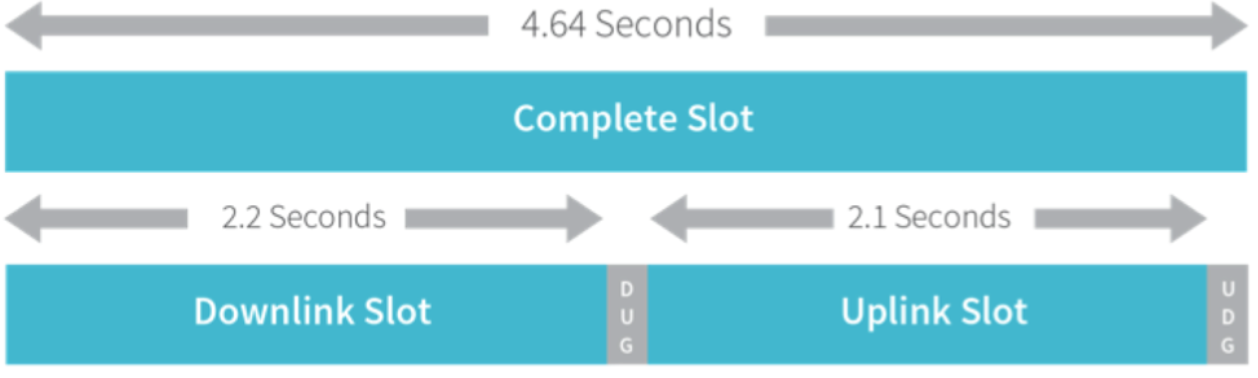
\includegraphics[width=\textwidth]{RPMASLOT.png}
\caption[Rpma slot]{Rpma slot}\label{fig:quarta}
\end{center}
\end{figure}
\\
Nella figura 1.4 \`e rappresentato il formato di uno slot RMPA. Lo slot in downlink precede quello in uplink permettendo di regolare la potenza di segnale in trasmissione dopo aver quantificato la potenza di segnale in downlink. 
Dato che la base station trasmette sempre in downlink alla stessa potenza, la potenza di segnale ricevuta \`e usata per calcolare quanto rumore c'\`e sul canale e quindi con quanta potenza deve essere inviato il messaggio in uplink. 
Se il canale \`e libero da interferenza il segnale ricevuto ha un buon livello di energia altrimenti se il canale \`e disturbato il segnale ricevuto ha una potenza inferiore.
RPMA non garantisce l'accesso al canale ai trasmettitori esattamente uno alla volta all'inizio di uno slot, pertanto riduce la sovrapposizione dei segnali trasmessi e cos\`i incrementa il rapporto segnale rumore sul singolo canale. 
Dal punto di vista del ricevitore, la base station utilizza pi\`u demodulatori per decifrare i segnali che arrivano in tempi diversi nello stesso slot. 
Ingenu fornisce comunicazioni bidirezionali con una leggera asimmetria nelle trasmissioni. 
Per le comunicazioni in downlink, la base station disperde i segnali per ciascun end-device e li diffonde usando CDMA.
RMPA raggiunge una soglia di sensitivit\`a di -142 dBm con un link budget di 168 dBm.  
Ingenu sta facendo diversi sforzi per adeguare il PHY layer allo standard IEEE 802.15.4k.
La tecnologia RPMA \`e compliant allo standard IEEE 802.15.4k \cite{K2}\cite{K6}.

\subsection{Telensa}
Telensa \`e un'azienda inglese che opera nell'ambito delle smart city ma soprattutto nel settore dell'illuminazione pubblica intelligente. 
Questa societ\`a ha sviluppato una tecnologia per applicazioni LPWAN progettando interamente lo stack di rete della soluzione proprietaria con il supporto all'integrazione di software di terze parti.
La soluzione sviluppata si basa su una tecnica di modulazione proprietaria UNB che usa la banda libera ISM con frequenze SUB-GHz. 
Non ci sono molti dettagli sull'implementazione della tecnologia wireless di Telensa, pertanto l'azienda si \`e posta come obiettivo di standardizzare la propria tecnologia usando usando le specifiche ETSI Low Throughput Networks (LTN) per una facile integrazione delle applicazioni.
Attualmente Telensa si \`e concentrata su ambiti applicativi molto specifici quali l'illuminazione intelliggente di cui dichiare essere leader e smart parking. 
Per rafforzare la propria posizione come leader di mercato dell'illuminazione pubblica intelligente, Telensa \`e confluita nel consorzio TALQ che si occupa del controllo e monitoraggio dell'illuminazione pubblica \cite{K2}.

\subsection{Qowisio}
Qowisio \`e una societ\`a francese operante nel settore delle telecomunicazioni che ha sviluppato una soluzione LPWAN dual stack che combina l'utilizzo di una tecnologia proprietaria UNB con LoRa. 
Essa fornisce connettivit\`a come servizio agli utenti finali.
La societ\`a fornisce sia gli end-device che l'infrastruttura, sviluppa applicazioni custom che si appoggiano su un sistema cloud di backend. 
Non esistono dettagli tecnici sull'implementazione delle proprie tecnologie \cite{K2}.

\subsection{Nwave}
La piattaforma Nwave ha la caratteristica di essere un sistema a ultra banda stretta RF (UNB), che opera nelle bande SUB-GHz ISM. 
L'architettura di rete \`e una topologia a stella che consente agevoli e dirette comunicazioni tra base station. Nwave ha come brand il sistema basato su ``advanced demodulation techniques'' che consente alla sua rete di coesistere con altre tecnologie radio senza rumore aggiuntivo\cite{K2}.

\subsection{Weightless}
Weightless \`e uno standard LPWAN aperto che realizza una piattaforma con l'obiettivo di diventare uno standard globale di riferimento consentendo l'innovazione attraverso software aperto. 
Come le altre tecnologie LPWAN, Weightless opera nella banda SUB-GHz. 
I suoi 3 standard aperti forniscono all'utente finale pi\`u scelte. 
Weightless-N offre un semplice standard direzionale ad una via con una lunga vita della batteria fino al 10 anni, unitamente ad un complessivo basso costo. La piattaforma Weightless offre anche la possibilit\`a di comunicazione a due vie, ma a fronte di una minore durata di vita delle batterie ed un pi\`u alto costo di gestione della rete. 
Weightless-W \`e l'opzione pi\`u estesa e opera fuori dello spettro TV inutilizzato, ma ha qualche svantaggio. 
La piattaforma Weightless ha complessivamente un ecosistema aperto, nel senso che ci sono pi\`u software aperti e venditori disponibili. Essa agisce come Weightless Special Interests Group (SIG), praticamente una organizzazione non-profit formata per lo sviluppo dei suoi standard aperti, nonch\`e per il test di imminenti tecnologie. Il suo pi\`u esteso standard aperto, ossia il Weightless-W, ha la caratteristica di una pi\`u breve durata della vita delle batterie (circa 3-5 anni) ed un pi\`u alto costo per il dispositivo terminale e per la rete. 
Come la Nwave, questa tecnologia \`e meno conosciuta\cite{K2}.


\chapter{LoRa e LoRaWAN}
LoRa \`e una delle tecnologie pi\`u interessanti che maggiormente contribuir\`a nei prossimi anni allo sviluppo delle LPWAN. Il termine LoRa \`e l'acronimo di Long Range  e si colloca nell'ambito di applicazioni WAN a bassa potenza.
LoRa \`e una tecnologia wireless proprietaria operante nella banda ISM (Industrial, Scientific and Medical) sviluppata dall'azienda francese Semtech Corporation. LoRa \`e un marchio sottoposto a brevetto, pertanto ogni altro produttore di componenti elettronici che volesse integrarla nei propri dispositivi dovr\`a corrispondere delle royalties alla casa francese. 
    
Spesso si sente parlare di LoRa e LoRaWAN indistintamente, ma \`e necessario fare distinzione tra i due termini.
LoRa \`e il livello fisico (o modulazione wireless) utilizzato per creare un link di comunicazione a lungo raggio attraverso questa tecnologia. Utilizza una tecnica di modulazione chiamata CSS (Chirp Spread Spectrum) utilizzata gi\`a da decenni in ambito militare e nelle comunicazioni aerospaziali, ma che \`e stata impiegata per la prima volta in ambito commerciale grazie a Semtech. 
LoRaWAN \`e il protocollo di comunicazione superiore a quello fisico con il quale vengono definite tutta una serie di regole e l'architettura della rete. I requisiti di progettazione di questo protocollo sono in linea con le caratteristiche definite per le LPWAN, ovvero il risparmio energetico dei dispositivi, la capacit\`a della rete, la qualit\`a del servizio, la sicurezza e la gestione di applicazioni vaste e variegate. 
La LoRa Alliance (https://www.lora-alliance.org/) \`e un'organizzazione non profit nata con lo scopo di standardizzare il protocollo e veicolare il successo a livello globale, i cui membri sono i maggiori leader del mercato, tra cui IBM, Google Cloud, Cisco, Orange, ST Microelectronics, Bouygues telecom e, ovviamente, Semtech.    
Lo scopo principale di LoRA, pertanto, \`e quello di permettere la comunicazione tra dispositivi su lungo raggio e con bassa potenza. LoRaWAN \`e in grado di colmare quel gap che sia le reti cellulari che le tecnologie come WiFi, BLE (bluetooth low energy) non sono in grado di soddisfare, in quanto le prime richiedono una elevata capacit\`a di banda e potenza trasmissiva mentre le seconde sono state pensate principalmente per ambienti indoor e per applicazioni a corto raggio. Le tecnologie basate su standard IEEE 802.15.4 come Zigbee, soddisfano il requisito di risparmio energetico ma non sono state progettate per trasmissioni a lungo raggio. Lo standard IEEE 802.15.4 adotta come soluzione al problema di copertura di una vasta aria, l'implentazione di una topologia di rete a mesh, che per\`o ha come svantaggio l'utilizzo di nodi che svolgono il compito di routing quindi devono essere sempre accesi.
\begin{figure}[h]                      
\begin{center} 
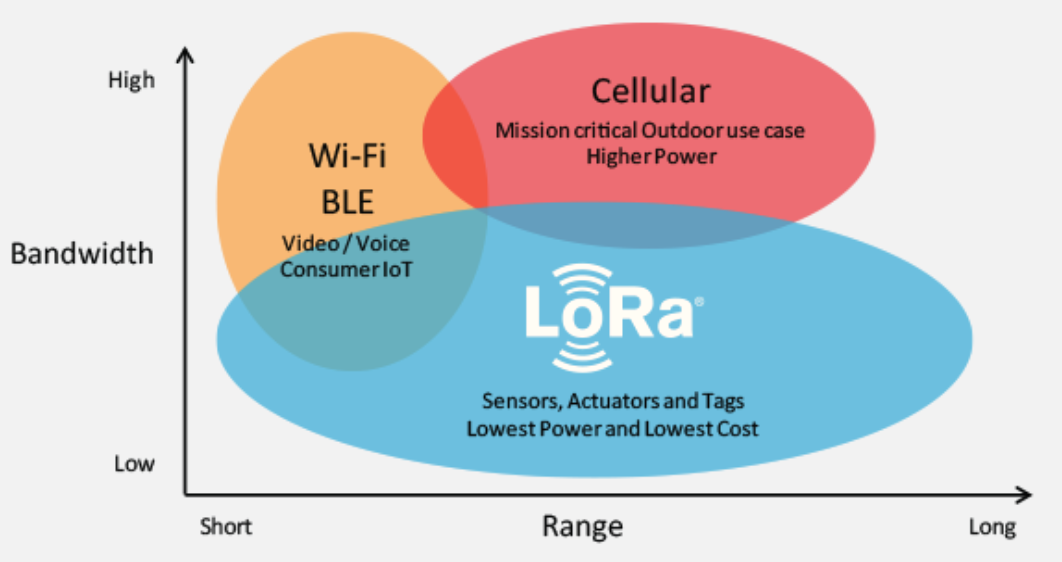
\includegraphics[width=\textwidth,height=55mm]{Lora_technology_gap.png}
\caption[Confronto tra LoRA e altre tecnologie wireless]{Confronto tra LoRA e altre tecnologie wireless}\label{fig:undicesima}
\end{center}
\end{figure}

\section{Panoramica tecnologia LoRa}
LoRa opera all'interno della banda ISM ovvero la porzione di spettro elettromagnetico riservato dall'ITU (International Telecommunication Union) alle applicazioni di radiocomunicazioni non commerciali, ma per uso industriale, scientifico e medico.
I requisiti normativi sono differenti in base ai vari continenti. Le due frequenze pi\`u diffuse sono 868 MHz in Europa e 915 MHz in Nord America. Altre regioni, in particolare l'Asia, hanno esigenze diverse. 
Queste frequenze, denominate Sub GigaHertz, hanno un'ottima capacit\`a di propagazione nello spazio e sono abbastanza resistenti agli ostacoli, pertanto si prestano bene agli ambiti in cui sono necessarie le trasmissioni a lungo raggio. Di contro, utilizzando una limitata ampiezza di banda, non consentono il trasporto di dati ad elevato bit rate.   
Una trasmissione LoRa pu\`o estendersi in campo aperto fino a 15 chilometri di distanza ed in ambito metropolitano fino ad un paio di chilometri. \cite{K20}
A livello fisico la tecnologia LoRa impiega, in Europa, 10 canali di trasmissione nella banda degli 867-869 Mhz. I canali hanno un'ampiezza di banda leggermente differente in base a che si tratti di canali in uplink (trasmissione di segnale) o downlink (ricezione di segnale). 
Nel primo caso l'ampiezza di banda \`e di 125/250 KHz, mentre nel secondo caso \`e di 125 KHz (in Europa).   

\begin{table}[h]                        
\begin{center}                          
\begin{tabular}{r|c|c}                  
$ $& $Europa$ & $Nord\ America$\\         
\hline\hline                                  
$Banda\ di frequenza$ & $867-869\ MHz$ & $902-928\ MHz$\\     
\hline                               
$Canali$ & $10$ & $64 + 8 +8$\\
\hline        
$BW\ canale\ uplink$ & $125/250 KHz$ & $125/500 KHz$\\ 
\hline 
$BW\ canale\ downlink$ & $125 KHz$ & $500 KHz$\\ 
\hline 
$Potenza\ TX\ uplink$ & $+14 dBm$ & $+20\ dBm\ tip.\ (+30\ dBm\ ammesso)$\\ 
\hline
$Potenza\ TX\ downlink$ & $+14 dBm$ & $+27 dBm $\\ 
\hline                                
$SF\ uplink$ & $7-12$ & $7-10$\\ 
\hline        
$Velocit\Grave{a}\ dati$ & $250 \sim 50\ kbps$ & $980 \sim 21,9\ kbps$\\ 
\hline 
$Bilancio\ collegamento\ uplink$ &$155 dBm$ & $ 154\ dBm$\\ 
\hline 
$Bilancio\ collegamento\ downlink$ &$155 dBm$ & $ 157\ dBm$\\ 
\hline \hline                         
\end{tabular}
\caption[Riepilogo caratteristiche spettro LoRA]{Riepilogo caratteristiche spettro LoRA}\label{tab:uno}
\end{center}
\end{table}



\section{LoRa PHY}
LoRa PHY (livello fisico) utilizza CSS (Chirp Spread Spectrum) come tecnica di dispersione dello spettro. 
Questa modulazione \`e stata sviluppata originariamente per applicazioni radar fin dagli anni '40 per poi essere adottata in diverse applicazioni di comunicazione di ambito militare. I punti di forza di questo tipo di modulazione sono la potenza relativamente bassa e l'elevata robustezza intrinseca a meccanismi di degrado del canale di comunicazione da interferenze come il multipath fading, l'effetto Doppler e l'in-band jamming. Essendo resistente all'effetto Doppler pu\`o essere anche impiegata per oggetti in movimento. 
CSS codifica i dati con un ``chirp'', essenzialmente un segnale sinusoidale modulato in frequenza a banda larga che varia linearmente con il tempo, crescendo (up-chirp) o decrescendo (down-chirp). 

\begin{figure}[h]                      
\begin{center} 
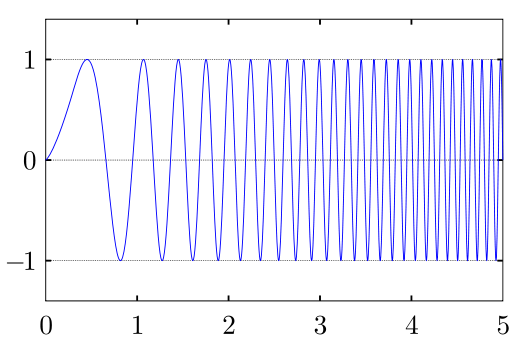
\includegraphics[width=\textwidth]{chirp_signal.png}
\caption[Rappresentazione di un chirp]{Rappresentazione di un chirp}\label{fig:tredicesima}
\end{center}
\end{figure}
CSS, a differenza di FHSS e DSSS, non aggiunge alcun elemento pseudo-casuale al segnale per aiutare a distinguerlo dal rumore sul canale, affidandosi invece alla natura lineare dell'impulso del chirp.  
La modulazione LoRa adopera pertanto una variazione di frequenza, concettualmente simile ad FSK (Frequency Shift Key) ma con uno schema un p\`o pi\`u complesso che rende la trasmissione pi\`u resiliente alle interferenze. L'intera banda di canale viene impiegata per la trasmissione. 
La bandwidth (BW) \`e la porzione di spettro occupata da un chirp, che nel caso di LoRa \`e scalabile ed \`e stata stabilita essere, in base agli accordi internazionali, di 125 Khz, 250 Khz e 500 Khz, anche se in Europa sono ammesse solo le prime due. Un incremento della banda permette di usare un data rate effettivo pi\`u alto, ma esistono dei vincoli normativi da rispettare in merito all'occupazione di banda.
Sebbene CSS \`e una tecnica di dispersione dello spettro e quindi garantisce una migliore qualit\`a di trasmissione, per poter garantire un buon compromesso tra performance ed impiego minimo di risorse i canali LoRa dispongono di una bandwidth ristretta \cite{K21}.
La modulazione spread spectrum LoRa viene eseguita attraverso la rappresentazione di ciascun bit dell'informazione del payload in pi\`u chirps di informazione. Il rate con il quale l'informazione viene diffusa ed inviata \`e relativa al symbol rate. Il rapporto tra il symbol rate nominale ed il chip rate \`e chiamato spreading factor e rappresenta il numero di simboli inviati per bit di informazione.  
Spreading Factor (SF) \`e ottenuto calcolando il logaritmo del numero di chirps per simbolo, in quanto 1 simbolo equivale a $2^{SF}$.
\\LoRa offre sei diversi fattori di dispersione che vanno da SF-7 a SF-12. Quanto pi\`u il fattore di dispersione \`e alto tanto pi\`u il segnale \`e robusto e sopravvive alle lunghe distanze.
Nella tabella 1.2 vengono riportati i valori di spreading factor ed il relativo numero di chips per simbolo.

\begin{table}[h]
\begin{center}
\begin{tabular}{lcccc}
&Spreading Factor&Chirps / Symbol&Lora Demodulator SNR\\ \hline\hline
&7&128&-7.5 db\\
\hline
&8&256&-10 db\\
\hline
&9&512&-12.5 db\\
\hline
&10&1024&-15 db db\\
\hline
&11&2048&-17.5 db\\
\hline
&12&4096&-20 db\\
\hline
\end{tabular}
\caption[Lora Spreading Factor, Chirps Symbol, Demodulator SNR]{Lora Spreading Factor, Chirps Symbol, Demodulator SNR}\label{tab:due}
\end{center}
\end{table}

Nella figura 1.8 \`e possibile apprezzare la differenza della durata di un chip in relazione ai valori di SF. Ad un valore pi\`u elevato di SF corrisponde una durata maggiore del segnale.  

\begin{figure}[h]                      
\begin{center} 
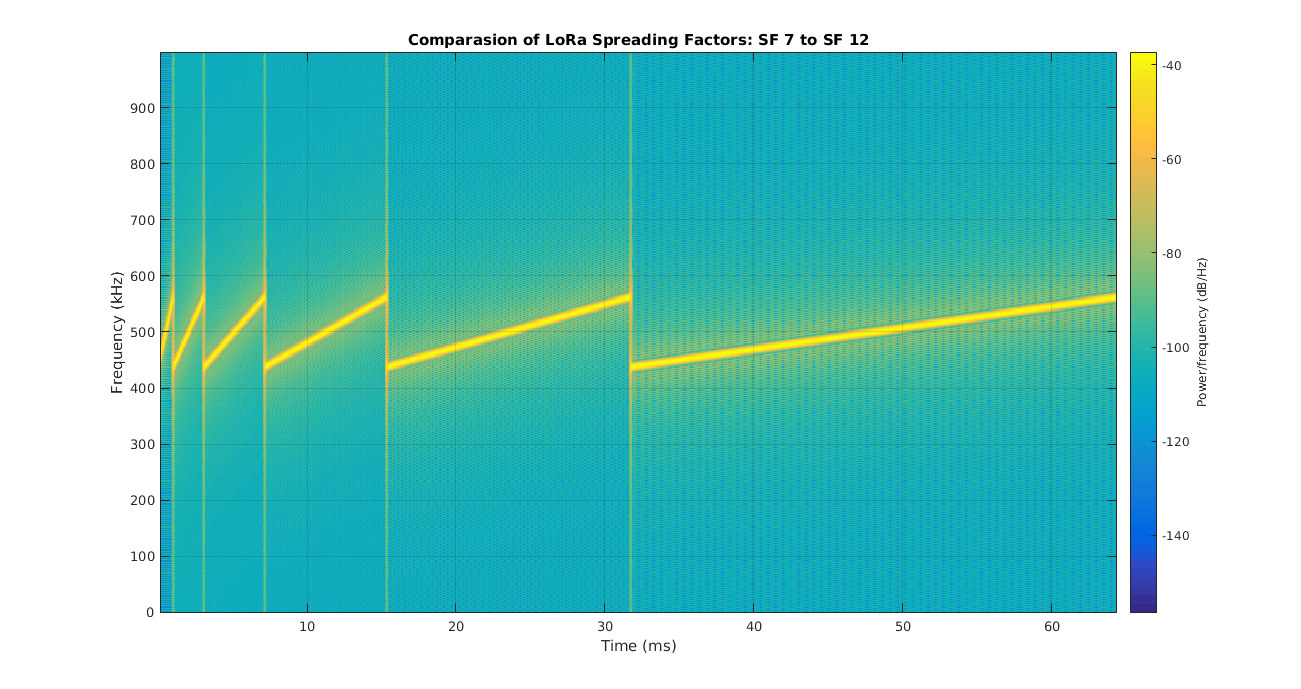
\includegraphics[width=\textwidth]{SF_Comparasion_7_12.png}
\caption[Spettrogramma dei diversi valori di Spreading Factor]{Spettrogramma dei diversi valori di Spreading Factor}\label{fig:prima}
\end{center}
\end{figure}

Il Chirp Rate rappresenta il numero il numero di chirp per secondo ed \`e equivalente alla BW \cite{K21}.
Il Coding Rate (CR) viene usato per migliorare la robustezza di un link LoRa ed indica il quantitativo di ridondanza applicata ai dati. Maggiore ridondanza equivale a fornire maggiore affidabilit\`a al trasporto dei dati a discapito del quantitativo di dati utili del payload. Esiste una relazione inversamente proporzionale tra ridondanza e bit rate. Il coding rate pu\`o assumere valori da 1 a 4.
Il modem LoRA impiega il controllo a ridondanza ciclica (CRC) per effettuare la correzione degli errori. Tuttavia la correzione degli errori introduce un overhead di dati relativo alla trasmissione. Il data overhead per trasmissione \`e riepilogato nella seguente tabella:

\begin{table}[h]
\begin{center} 
\begin{tabular}{lcccc}
&Coding Rate&Cycle Coding Rate&Overhead Radio\\ \hline\hline
&1&4/5&1.25\\
\hline
&2&4/6&1.5\\
\hline
&3&4/7&1.75\\
\hline
&4&4/8&2\\
\hline
\end{tabular}
\caption[Lora Coding Rate, Cycle Coding Rate,Overhead Radio]{Lora Coding Rate, Cycle Coding Rate,Overhead Radio}\label{tab:tre}
\end{center}
\end{table}


 Un simbolo nella modulazione CSS ha quattro importanti parametri: Spreading Factor, frequenza minima $f_{min}$, frequenza massima $f_{max}$, input bits. Per generare un simbolo CSS, \`e necessaria una frequenza di partenza f0. La frequenza di partenza  \`e compresa tra $f_{min}$ e $f_{max}$ e rappresenta l'informazione in input ottenuta con $log_2(SF)$. Per $SF^1$,  $log_2(SF)$ bits definisco  $f_0$. 
 \\La lunghezza di un simbolo $T_s$ pu\`o essere cos\`i calcolata:
 
 
\begin{equation*} T_s = \frac{2^{SF}}{BW} = \frac{2^{SF}}{f_{max}-f_{min}}\end{equation*}

Una volta che  la lunghezza di un simbolo $T_s$ \`e stata definita, possiamo definire un chirp come un tono che oscilla tra $f_0$ e $f_{max}$.
La modulazione LoRa \`e definita attraverso tre parametri: Spreading Factor (SF), bandwidth (BW) e frequenza del canale. Il compito svolto dal modulatore \`e quello di tradurre i simboli costituiti da SF bits in chirps che corrispondono a $2^{SF}$ samples ad un specifico chirp rate (BW).  Pertanto i bits di SF del simbolo in ingresso si traducono in $2^{SF}$ spostamenti unici dell'onda base che rappresenta il chirp.
Un aspetto importante della modulazione CSS \`e che per ogni simbolo \`e necessario raddoppiare il numero di samples in output necessari per modulare il simbolo. Questo rende la modulazione LoRa CSS molto lenta ma estremamente robusta alle interferenze ed al rumore. 

Il fattore di dispersione SF, la bandwidth BW ed il coding rate determinano Il bit rate della trasmissione dati LoRa :

\begin{equation*} T_s = SF * \frac{\tfrac{4}{4+CR}}{\tfrac{2^{SF}}{BW}} * 1000 = SF * \frac{BW}{2^{SF}} * CR * 1000 \end{equation*}

Dove:
\begin{itemize}                       
\item SF = Spreading Factor (6,7,8,9,10,11,12)
\item CR = Coding Rate (1,2,3,4)
\item BW = Bandwidth in KHz (10.4, 15.6, 20.8, 31.25, 41.7, 62.5, 125, 250, 2500)
\item $R_b$= Data rate or Bit Rate in bps 
\end{itemize}
Il bit rate in LoRa dipende dalla combinazione dei possibili valori di SF, CR e BW, pertanto si pu\`o calcolare quali sono i data rate possibili.
Il rapporto che esiste tra spreading factor e bit rate \`e inversamente proporzionale. Se si vogliono raggiungere distanze maggiori bisogna aumentare spreading factor a discapito del bit rate, viceversa se si vuole incrementare data rate bisogna ridurre spreading factor. Nella tabella 4.4 riporto un esempio del data rate ottenibile per le tre differenti bande a parit\`a di spreading factor e coding rate. 
\\
\begin{table}
\begin{center}
\begin{tabular}{lcccc}
&Bandwidth (KHz)&Spreading Factor&Coding Rate&Nominal $R_b$ (bps)\\ \hline\hline
&125&7&4/5&5470\\
\hline
&250&7&4/5&11000\\
\hline
&500&7&4/5&21875\\
\hline
&125&12&4/5&293\\
\hline
&250&12&4/5&586\\
\hline
&500&12&4/5&1172\\
\hline
\end{tabular}
\caption[Lora Bandwidth (KHz), Spreading Factor, Coding Rate, Nominal $R_b$ ]{Lora Bandwidth (KHz), Spreading Factor, Coding Rate, Nominal $R_b$ }\label{tab:quattro}
\end{center}
\end{table}
\\
\\
In base ai requisiti dell'applicazione, ma soprattutto in base allo scenario in cui vengono collocati due stazioni che trasmettono attraverso un link Lora \`e possibile configurare i parametri di spreading factor, coding rate e bandwidth per ottenere le migliori condizioni per la qualit\`a di servizio.
Tra le features pi\`u interessanti di LoRa c'\`e anche l'elevata sensitivit\`a, in quanto la stazione radio \`e in grado di decifrare il segnale fino alla soglia di -137 dBm. Grazie all'elevata sensitivit\`a, LoRa \`e in grado di ricevere e trasmettere dati anche su distanze dell'ordine dei chilometri. Esiste un rapporto diretto tra spreading factor, bandwidth e la soglia di sensitivit\`a possibile in relazione a questi due fattori. 
Spreading Factor rappresenta il rapporto tra chip rate e symbol rate, pertanto per un valore alto di SF corrisponde un incremento del Signal Noise Ratio (SNR), della sensitivit\`a, della distanza ma anche tempo necessario alla trasmissione del dato (airtime).
SNR \`e il rapporto minimo tra potenza del segnale desiderata e rumore che pu\`o essere demodulato e viene espressa in db. Per il calcolo della sensibilit\`a del ricevitore, \`e necessario il valore SNR minimo in modo che l'informazione possa essere decodificata correttamente. Ad ogni valore di spreading factor corrisponde una soglia minima di SNR. Ad esempio per un valore di SF pari a 7 \`e necessario un valore minimo di -7.5 db di SNR per decifrare l'informazione. Questi valori possono cambiare anche in base alla BW. La tabella seguente riepiloga la corrispondenza che esiste tra SF, SNR e time on air sulla banda dei 125 KHz. 
Bisogna precisare che il time on air dipende anche dalla dimensione in byte del pacchetto inviato \cite{K21}. 

\begin{table}
\begin{center}
\begin{tabular}{cccccc}
Spreading Factor&SNR Limit (db)&Time on air (10 byte packet)\\ \hline\hline
7&-7.5 &56 ms\\
\hline
8&-10&103 ms\\
\hline
9&-12.5&205 ms\\
\hline
10&-15&371 ms\\
\hline
11&-17.5&741 ms\\
\hline
12&-20&1483 ms\\
\hline
\end{tabular}
\caption[Lora Spreading Factor,SNR Limit (db),Time on air]{Lora Spreading Factor,SNR Limit (db),Time on air}\label{tab:quattro}
\end{center}
\end{table}



La soglia di sensitivit\`a di un ricevitore radio indica il valore espresso in db al di sotto del quale non \`e possibile decodificare i dati trasmessi. 
La formula per calcolare la sensitivit\`a S, di un ricevitore radio \`e la seguente:
\begin{equation*} S = -174 + 10log_{10}(BW) + NF + SNR  \end{equation*}

Dove:
\begin{itemize}                       
\item S = sensitivit\`a in dBm
\item BW = Bandwidth in KHz
\item NF = Noise Figure (quantifica la rumorosit\`a di un sistema)
\item SNR = Signal Noise Ratio
\end{itemize}
L'equazione della soglia di sensitivit\`a prende in considerazione il valore di SNR, pertanto essendo quest'ultimo, nel caso di LoRa in riferimento a SF, ne consegue che esiste un valore di sensitivit\`a diverso per ogni valore di SF. Anche in questo caso per un pi\`u alto valore di SF corrisponde un pi\`u alto valore di SNR e quindi \`e necessaria una sensitivit\`a maggiore. 
La tabella seguente mostra quali sono i valori di sensitivit\`a in relazione ai valori di SF per ogni banda di frequenza \cite{K21}.
\\
\begin{table}
\begin{center}
\begin{tabular}{cccccc}
Spreading Factor&BW = 125 KHz&BW = 250 KHz&BW = 500 KHz\\ \hline\hline
7&-126.50&-124.25&-120.75\\
\hline
8&-127.25&-126.75&-124.00\\
\hline
9&-131.25&-128.25&-127.50\\
\hline
10&-132.75&-130.25&-128.75\\
\hline
11&-134.50&-132.75&-128.75\\
\hline
12&-133.25&-132.25&-132.25\\
\hline
\end{tabular}
\caption[Rapporto tra Spreading Factor e Bandwidth]{Rapporto tra Spreading Factor e Bandwidth}\label{tab:cinque}
\end{center}
\end{table}


La modulazione LoRa implementata dal livello PHY fornisce un importante miglioramento di link budget rispetto alle tradizionali modulazioni narrowband. 
Il link budget massimo \`e di 157 dB e viene calcolato in questo modo \cite{K22} :

\begin{itemize}                       
\item $P_{rx}$ = +20 dBm a 100 mW costanti in output all'antenna
\item RS = fino a -137 dBm
\item LB = +20 -(-137) = +157 dB
\end{itemize}

Il livello fisico LoRa (PHY Layer) oltre a definire tutte le caratteristiche per la modulazione del segnale, definisce anche la struttura del pacchetto. 
BW e SF sono i principali parametri della modulazione LoRa. Un simbolo LoRa \`e composto da $2^{SF}$ chirps, che coprono l'intera banda a disposizione. Un chirps a livello fisico, inizia con una serie di upward chirps (variazione crescente della frequenza). 
La variazione di frequenza nel tempo viene effettuata quando viene raggiunta la frequenza massima della banda per poi ripartire dalla frequenza minima, come \`e possibile vedere in fugura 1.13.


\begin{figure}[h]                      
\begin{center} 
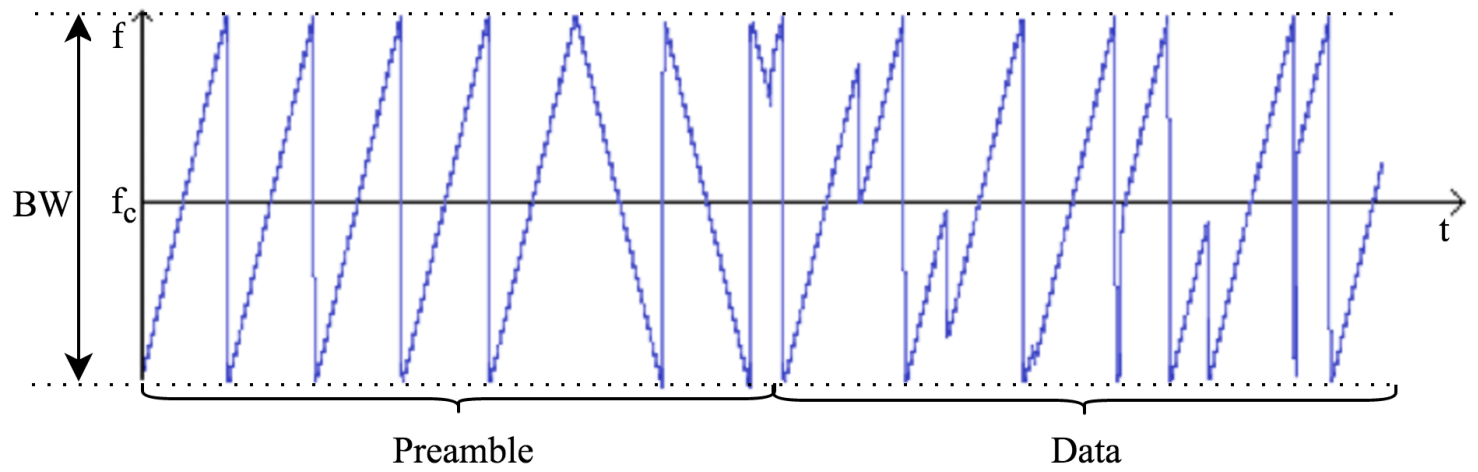
\includegraphics[width=\textwidth]{lora_frequency_variation.png}
\caption[Variazione di frequenza nel tempo di un segnale LoRa]{ Variazione di frequenza nel tempo di un segnale emesso. $f_c$ \`e la frequenza centrale del canale.}\label{fig:prima}
\end{center}
\end{figure}

Sebbene la modulazione LoRa potrebbe trasmettere un qualsiasi frame, Semtech definisce uno specifico formato del frame per la trasmissioni di un pacchetto tra due stazioni LoRa.
Un frame LoRa inizia con un preambolo. Il preambolo inizia con una sequenza costante di otto up-chirps che coprono l'intera banda di frequenza. Gli ultimi due up-chirps dell'ottetto, decodificano la sync word. La sync word \`e un valore di un byte che \`e usato da differenti LoRa network che usando la stessa banda. Un dispositivo configurato con una specifica sync word potr\`a fermare l'ascolto delle trasmissioni se si accorge che la sync word non corrisponde alla sua configurazione. 
Dopo gli otto up-chirps seguono due down-chirps pi\`u 1/4 di down-chirp, per una durata di 2.25 simboli chiamati simboli di sincronizzazione che vengono usati per la sincronizzare la trasmissione nel tempo. La durata totale del preambolo pu\`o essere configurata tra 10.25 e 65539.25 simboli. A seguire c'\`e la trasmissione dei simboli che identificano il payload.
L'immagine sottostante mostra la modulazione del segnale di un frame LoRa.

\begin{figure}[h]                      
\begin{center} 
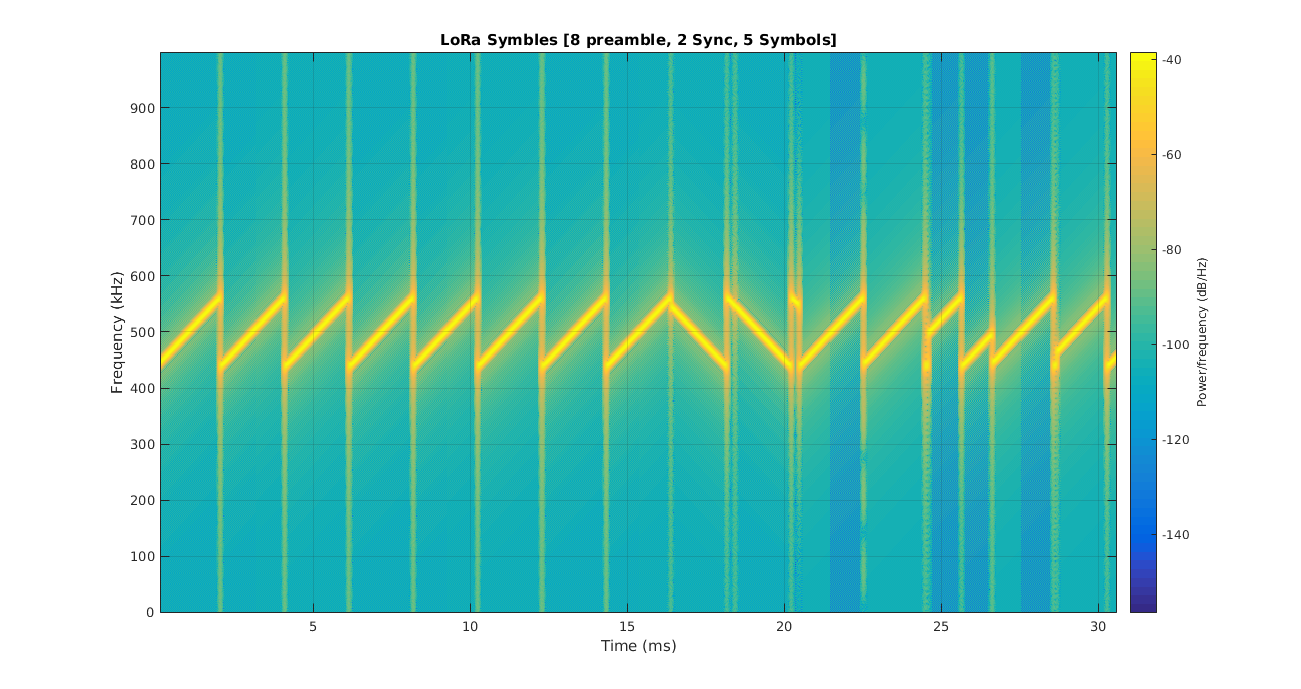
\includegraphics[width=\textwidth]{LoRa_Symbols_01.png}
\caption[Spettrogramma LoRa]{ Spettrogramma LoRa}\label{fig:prima}
\end{center}
\end{figure}

Dopo il preambolo c'\`e un header opzionale. Quando \`e presente, questo header \`e trasmesso con un code rate di 4/8. Questo indica la dimensione del payload (in byte), il code rate usato per la fine della trasmissione e se il CRC a 16-bit \`e abilitato o meno, quindi se presente dopo il payload. L'header, inoltre, include un CRC che permette al receiver di scartare i pacchetti con un header non corretto. Il payload pu\`o avere dimensioni da 1 a 255 byte. L'header pu\`o essere disabilitato se ritenuto non opportuno usarlo per lasciare un maggiore spazio per il payload. Il payload \`e sempre inviato dopo l'header e alla fine del frame pu\`o esserci opzionalmente il CRC del payload. 
Nell'immagine sottostante lo schema che riassume il formato del frame:

\begin{figure}[h]                      
\begin{center} 
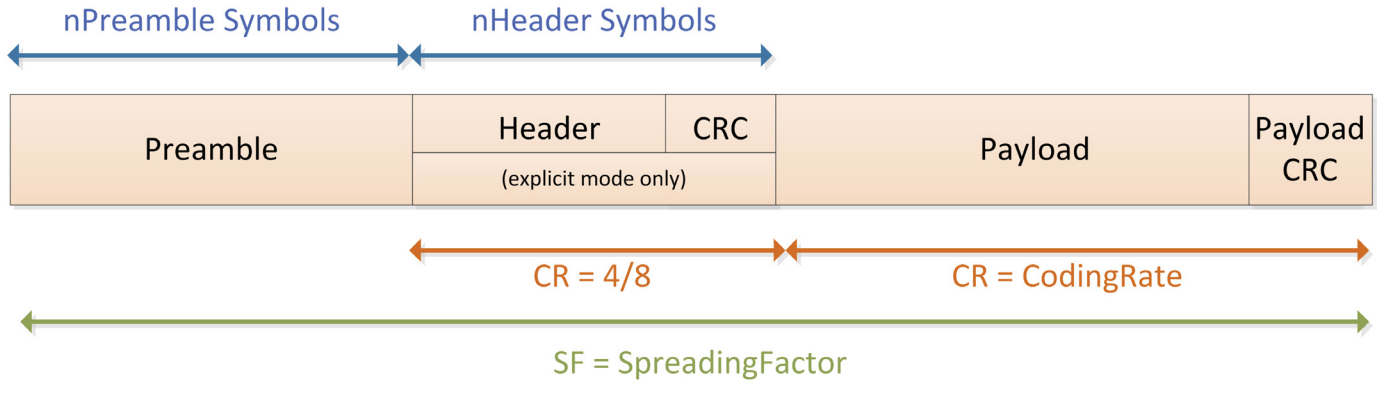
\includegraphics[width=\textwidth]{struttura_pacchetto_lora.png}
\caption[Struttura di un frame LoRa]{ Struttura di un frame LoRa.} \label{fig:venti}
 %\begin{equation*} CR = \tfrac{4}{(4+n)}con  n \in \{1..4\}\end{equation*}
\end{center}
\end{figure}

Per trasmettere il payload $n_s$ \`e possibile calcolare quanti simboli sono necessari attraverso un equazione che prende in considerazione tutti questi parametri. Per calcolare quanti sono i simboli necessari per la dimensione totale del pacchetto bisogna aggiungere anche i simboli per codificare il preambolo. L'equazione  \`e la seguente :

\begin{equation*} n_s = 8 + max (\frac{8PL-4SF+8+CRC+H}{4 * (SF-Df)} * \frac{4}{CR},0) \end{equation*}
Dove:
\begin{itemize}                       
\item PL = dimensione payload in byte
\item CRC = 16 se il CRC \`e abilitato, zero altrimenti
\item H = 20 quando l'header \`e abilitato, zero altrimenti
\item DE = 2 quando low data rate optimization \`e abilitato, zero altrimenti
\end{itemize}


\section{LoRaWAN}
LoRaWAN \`e il protocollo di livello MAC creato per usare lo strato fisico LoRa. Esso \`e stato progettato principalmente per le reti di sensori, in cui i dispositivi scambiano pacchetti con un server con un basso data rate e con un lungo intervallo di tempo. 
Lo stack LoRaWAN \`e composto da quattro livelli. Al livello pi\`u basso c'\`e la specifica inerente l'accesso fisico alle frequenza della banda ISM e le relative regolamentazioni che dipendono dall'area geografica in cui si opera. Il secondo livello c'\`e la specifica sulla modulazione LoRa e rappresenta lo strato proprietario di Semtech, in quanto la tecnica di CSS utilizzata da LoRa \`e stata brevettata. Il livello Mac \`e open source e definisce le classi degli end-device. Il livello pi\`u alto \`e l'applicazione in cui il dispositivo viene impiegato.

\begin{figure}[h]                      
\begin{center} 
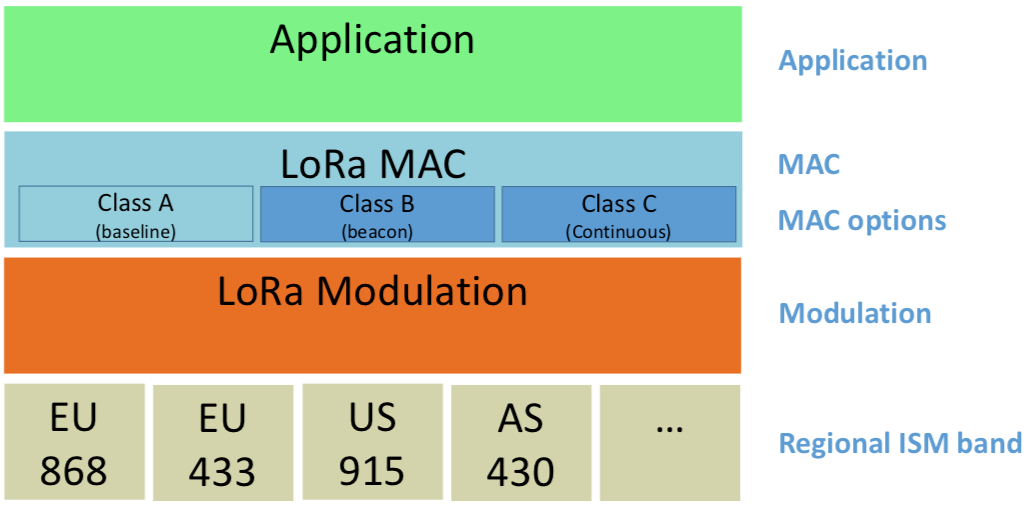
\includegraphics[width=\textwidth]{lorawan_protocolo_stack.png}
\caption[Stack LoRaWAN]{Stack LoRaWAN} \label{fig:venti}
\end{center}
\end{figure}
LoRAWAN definisce la topologia della rete e quali sono i ruoli dei dispositivi in questo contesto. 
La topologia della rete LoRaWAN \`e a stella in cui vi \`e un nodo centrale con la funzione di gateway in grado di instradare verso la rete Internet tutti i pacchetti provenienti dai vari dispositivi con cui interagisce attraverso un link LoRa entro il raggio di copertura della trasmissione. In questo design non \`e previsto che i dispositivi possano comunicare direttamente tra loro e tantomeno possano instradare i pacchetti verso altri nodi. Questa scelta progettuale fa in modo che sebbene l'architettura di rete sia abbastanza semplice ed il nodo gateway rappresenta un single point of failure permette di mantenere i costi di deploy bassi, in quanto i dispositivi hanno solo il ruolo di trasmettere e ricevere dati verso il gateway e vengono assolti dalle funzioni di routing tipico delle reti mesh. 

\section{Componenti di una rete LoRaWAN}
Nelle specifiche del protocollo LoRaWAN vengono definiti i ruoli dei componenti all'interno della rete: end-device, gateway e network server.
Gli end-device sono sensori a basso consumo energetico in grado di comunicare con il gateway attraverso un link LoRa. All'interno di una rete LoRa possono essere presenti anche migliaia di questi nodi in quanto questi dispositivi possono trasmettere anche allo stesso tempo sul mezzo trasmissivo usando differenti frequenze o spreading factor.

Il gateway : dispositivo intermedio in grado di instradare i pacchetti provenienti dagli end-device verso il network server attraverso un collegamento IP che possa permettere un elevato throughput come ad esempio un link 3g/4g oppure Ethernet. In un deploy LoRaWAN possono esistere pi\`u gateways e lo stesso pacchetto pu\`o essere ricevuto ed instradato da uno o pi\`u gateway. Per poter supportare una rete a stella di ampie dimensioni il gateway deve disporre di buone capacit\`a e disponibilit\`a di ricevere un alto numero di messaggi provenienti da un elevato numero di end-device (anche sull'ordine delle migliaia). Il gateway \`e in grado di ascoltare le trasmissioni anche su pi\`u canali e di decodificare pacchetti inviati con un differente spreading factor anche contemporaneamente. 

Il network server \`e una componente di back-end che svolge processi pi\`u complessi in relazione al management del network.
Esso \`e responsabile della ricezione dei pacchetti dai vari gateway e svolge diverse funzionalit\`a tra cui il filtraggio ed eliminazione di eventuali pacchetti duplicati. Il network server implementa la funzionalit\`a di adaptive data rate (ADR) allo scopo di massimizzare la vita delle batterie degli end-points e la capacit\`a totale della rete. Il network server assegna a ogni end-points che si vuole connettere alla rete, un data rate e una potenza di uscita da utilizzare per la trasmissione RF, diversa per ogni esigenza. L'algoritmo ADR assegna un data rate maggiore ai nodi terminali pi\`u vicini al gateway in quanto meno suscettibili alle interferenze, e una potenza di uscita minore per la trasmissione RF. Minor tempo di trasmissione e minor potenza di uscita si traducono in un ovvio risparmio energetico. Solo ai nodi che si trovano a distanze notevoli dal gateway, il server assegner\`a un data rate pi\`u basso (minore suscettibilit\`a ai rumori) e una maggiore potenza di uscita. Il data rate previsto dagli end-points non \`e quindi costante. Le specifiche LoRaWAN indicano valori che vanno da 300bps fino a 50kbps \cite{K22}.

I dati ricevuti possono essere inviati agli application server per le elaborazioni successive oppure \`e possibile inviare eventuali notifiche agli end device per far attuare un'azione. Non ci sono interfacce standard di trasmissione dei dati tra network server ed application server.

\begin{figure}[h]                      
\begin{center} 
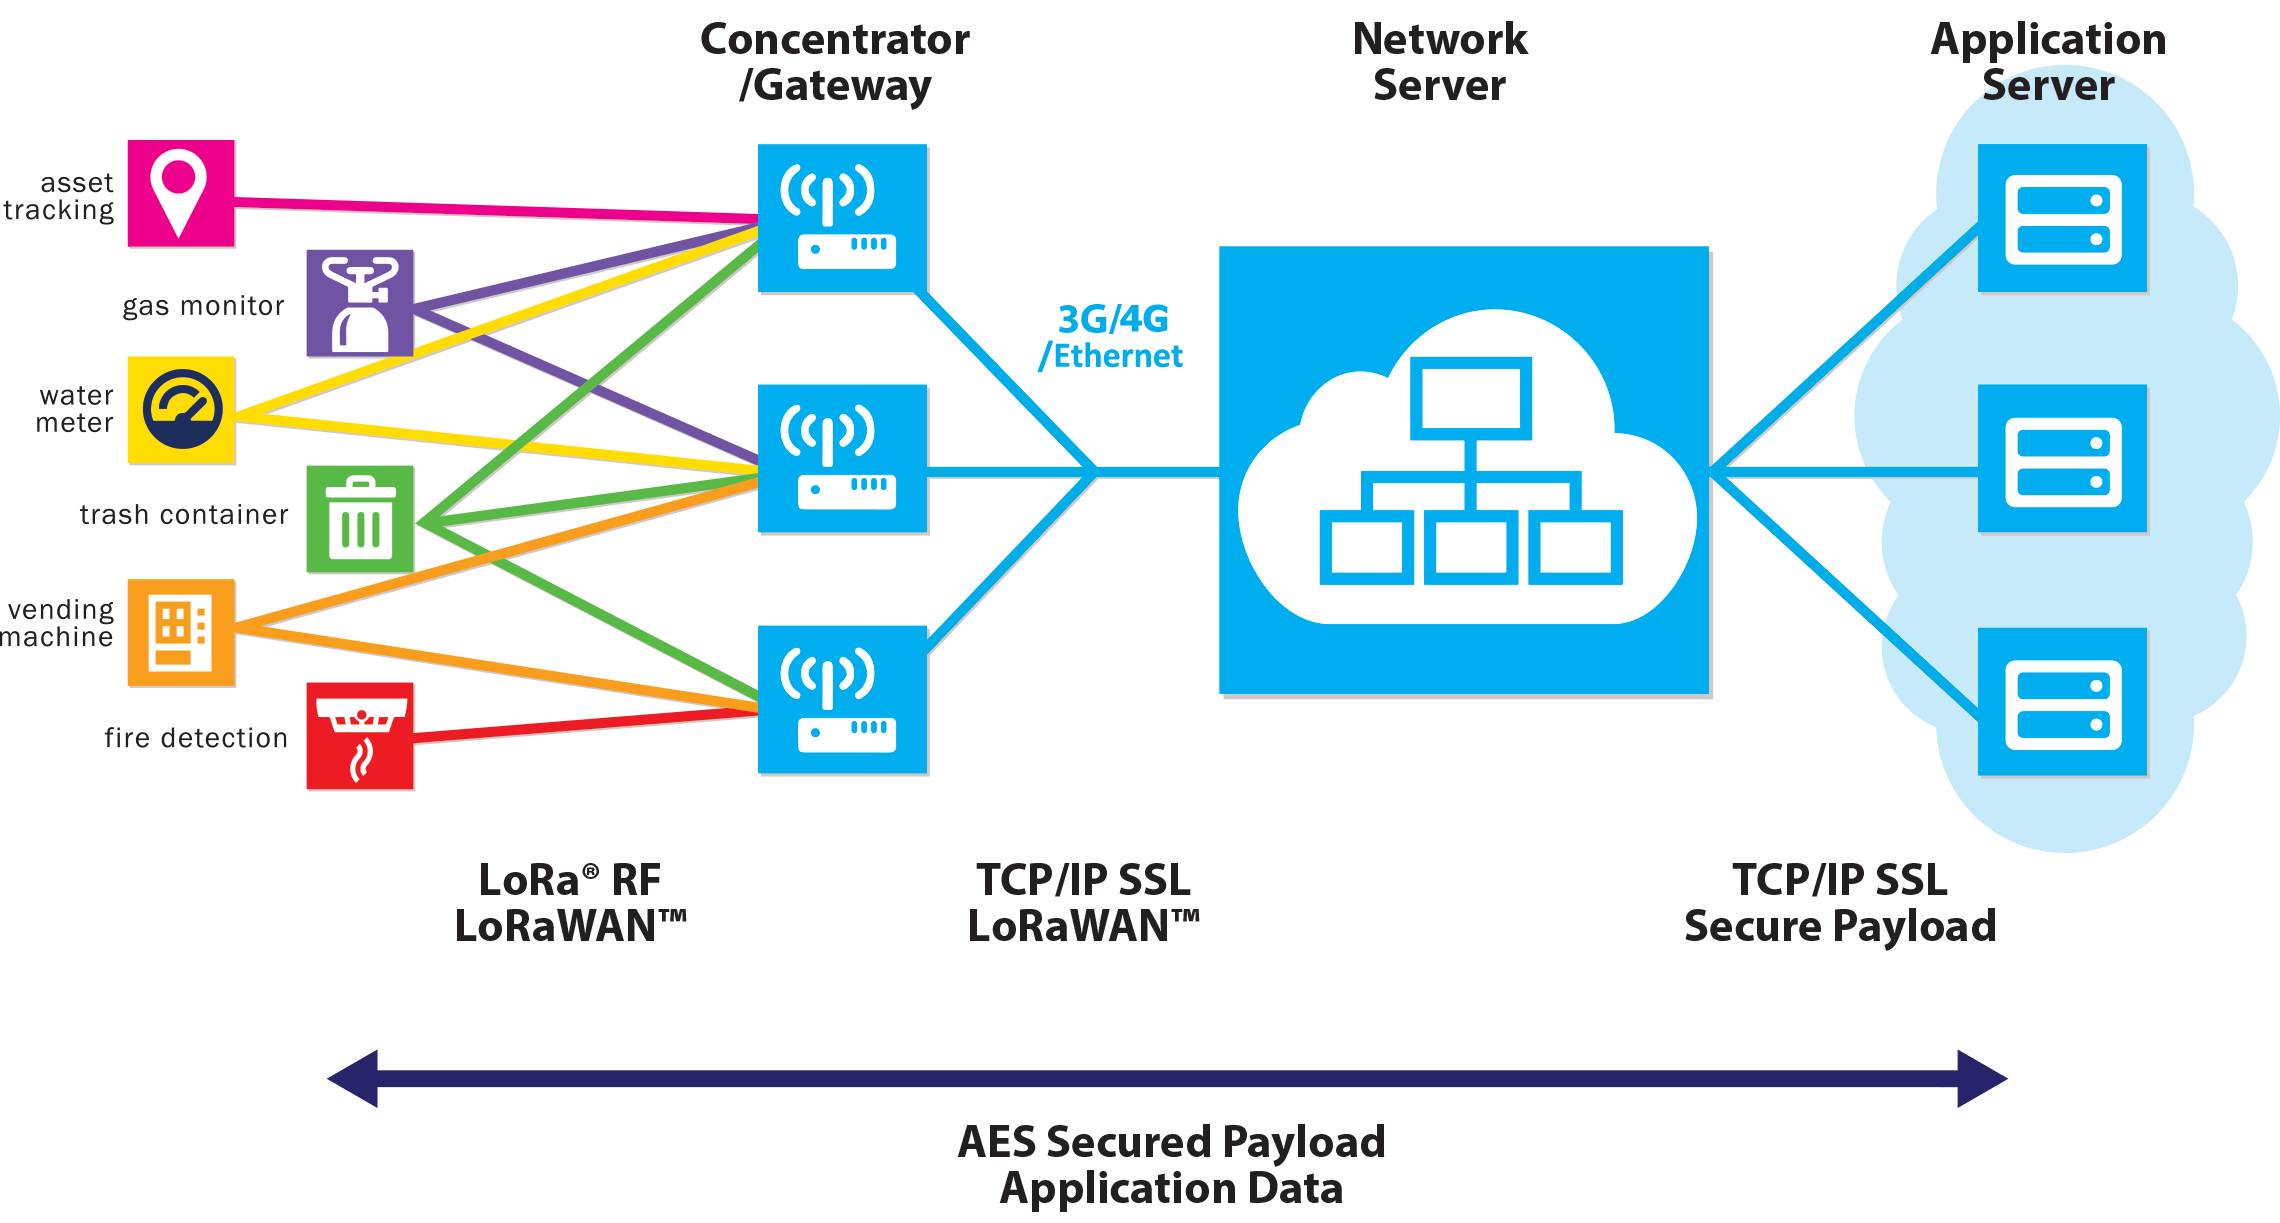
\includegraphics[width=\textwidth]{tologia-lorawan.png}
\caption[Architettura LoRaWAN]{Architettura LoRaWAN} \label{fig:venti}
\end{center}
\end{figure}

A differenza di una tradizionale rete cellulare o una rete Wi-Fi, gli end-device non sono associati ad uno specifico gateway per poter accedere alla rete. Il gateway ha semplicemente il ruolo di stabilire un link di comunicazione LoRa e di instradare i pacchetti ricevuti dagli end-device verso il network server e viceversa, al pi\`u aggiungendo informazioni sulla qualit\`a di ricezione dei dati. In questo modo, un end-device \`e associato ad un network server il quale rappresenta una sorta di coordinatore della rete ed \`e in grado di comunicare con un end-device attraverso il gateway opportuno. A livello logico il gateway \`e trasparente in quanto ha solo il ruolo di instradamento senza fare alcuna elaborazione.
Le trasmissioni tra end-device e gateway possono essere di due tipi :
\begin{itemize}                       
\item Uplink : trasmissione dati da end-device verso il gateway
\item Downlink : trasmissione dati da gateway verso end-device
\end{itemize}
LoRaWAN ha tre differenti classi di end-device che si differenziano tra loro sulla modalit\`a di ricezione dei pacchetti in downlink (da gateway verso end-device). In questo modo \`e possibile soddisfare i requisiti di scenari applicativi differenti in relazione al consumo energetico. Di default i dispositivi LoRa operano in modalit\`a classe A con le propriet\`a di risparmio energetico, mentre devono essere esplicitamente configurati per operare in classe B o C. Inoltre i dispositivi di classe B e C devono comunque soddisfare anche i requisiti di classe A \cite{K22}.
Le tre classi dei dispositivi sono:
\begin{itemize} 
\item  Classe A, bidirezionali: I dispositivi di classe A possono schedulare l'invio di una trasmissione in uplink in base alle specifiche dell'applicazione ad intervalli di tempo regolari con un piccolo jitter che consiste in una variazione random prima della trasmissione. Questi tipi di device permettono comunicazioni bidirezionali attraverso un meccanismo per il quale restano in ascolto per un certo intervallo di tempo di eventuali trasmissioni in downlink solo dopo aver effettuato una trasmissione in uplink. Il tempo in cui restano in ascolto \`e determinato da due brevi finestre in ricezione dopo aver trasmesso un pacchetto. Una volta terminato il tempo di ricezione il dispositivo di classe A torna in modalit\`a dormiente per conservare energia delle batterie.



\item Classe B, bidirezionali con slot in ricezione schedulato : Questi tipi di dispositivi si mettono in ascolto di comunicazioni in downlink aprendo una finestra in ricezione ad intervalli di tempo schedulati. Per questo tipo di comunicazione \`e necessario un meccanismo di sincronizzazione con il gateway che avviene mediante beacon. Il network server dovr\`a conoscere quando l'end-device sar\`a in ascolto. 

\item Classe C, bidirezionali con con slot di ricezione: A questa categoria afferiscono tutti quei dispositivi che sono costantemente in ascolto. Il ricevitore LoRA resta costantemente in ascolto permettendo una ricezione immediata senza che il dispositivo apra una finesta in ascolto. 
\end{itemize}

\begin{figure}[h]                      
\begin{center} 
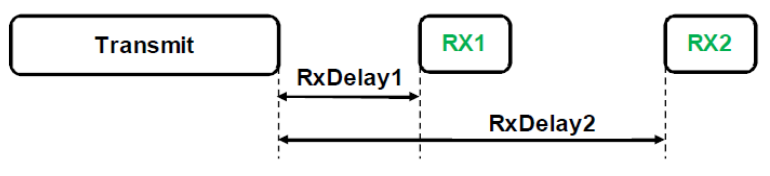
\includegraphics[width=\textwidth]{CLASSE-A_receive-window.png} 
\caption[LoRa device classe A]{Classe A}\label{fig:venti}
\end{center}
\end{figure}


\begin{figure}[h]                      
\begin{center} 
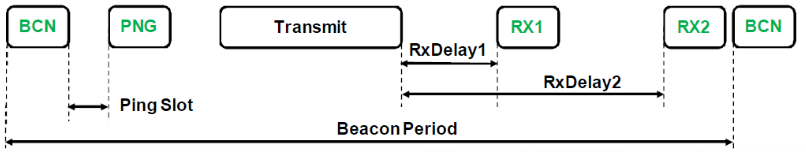
\includegraphics[width=\textwidth]{CLASSE_B_receive-window.png} 
\caption[LoRa device classe B]{ Classe B}\label{fig:venti}
\end{center}
\end{figure}


\begin{figure}[h]                      
\begin{center} 
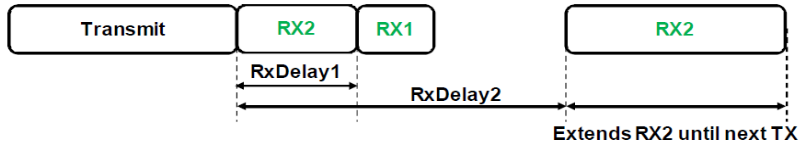
\includegraphics[width=\textwidth]{CLASSE_C_receive-window.png} 
\caption[LoRa device classe C]{ Classe C}\label{fig:venti}
\end{center}
\end{figure}

La scelta della classe dell'end-device deve essere ponderata in base ai requisiti dell'applicazione ed al contesto in cui si opera. Le classi A e B garantiscono una migliore efficienza energetica e sono stati pensati per i dispositivi alimentati a batteria, mentre gli end-device di classe C sono alimentati attraverso rete elettrica e che possono attivare una finestra di ricezione stando perennemente in ascolto. Questo tipo di comunicazione non \`e pensato per il risparmio energetico ma garantisce che il dispositivo possa ricevere direttive in un qualsiasi momento. 
La banda ISM utilizzata dalle reti LoRaWAn \`e soggetta a limitazioni d'uso sulla base delle normative vigenti. Esistono delle regolamentazioni in merito alla potenza massima trasmissiva e sul duty cycle (ciclo di lavoro utile). Le limitazioni sul duty cycle si traducono in un ritardo sul frame che deve essere successivamente inviato. 
In Europa sulla banda di frequenza degli 868 MHz il duty cycle \`e pari a 1\% per gli end-device \cite{K27}.  Questo implica che un end-device su 100 slot di tempo (suddivisione logica del tempo) ne pu\`o impiegare al pi\`u uno per la trasmissione. Inoltre dovr\`a effettuare un salto di canale pseudo-random per ogni trasmissione. Infine, nelle public community network, esiste un regolamento per una equa politica di accesso al canale che limita la trasmissione in uplink a 30 secondi al giorno per end-device ed i messaggi in down-link a 10 messaggi al giorno per end-device. Tuttavia se si una una rete LoRaWAN privata non sono previste queste limitazioni ma bisogna rispettare i limiti imposti dalle leggi governative. 
Per quanto riguarda la politica di accesso al canale condiviso da parte di pi\`u stazioni trasmittenti, LoRa non implementa nessun meccanismo di channel feedback ovvero di ascoltare il canale prima di trasmettere per verificare se \`e occupato da un'altra trasmissione come avviene invece per il protocollo CSMA. I dispositivi di classe A implementano una politica di accesso al mezzo simile ad ALOHA, in cui il tempo \`e suddiviso in intervalli logici (slot) di lunghezza prefissata. La trasmissione del dato sul canale avviene quando il trasmettitore radio \`e pronto dopo aver aspettato per un numero casuale di slots. Viene inviato sempre il primo pacchetto in testa alla coda del buffer. Nel caso di messaggi che richiedono conferma (ack) il trasmettitore effettua una ritrasmissione in caso di mancata ricezione di ack.  

\section{Formato dei pacchetti LoRaWAN}
LoRaWAN utilizza a livello fisico il formato del frame descritto nella sezione precedente. Header e CRC sono obbligatori per i messaggi in uplink, per questo motivo \`e impossibile usare un valore di spreading factor pari a sei in quanto non ci sarebbero sufficienti simboli per la rappresentazione del dato durante la trasmissione. I messaggi in downlink hanno l'header, ma non hanno il CRC. 
La dimensione massima di un header MAC \`e di 13 byte, mentre la dimensione massima \`e di 28 byte.
Nell'immagine seguente si mostra il formato del messaggio nel dettaglio : 

\begin{figure}[h]                      
\begin{center} 
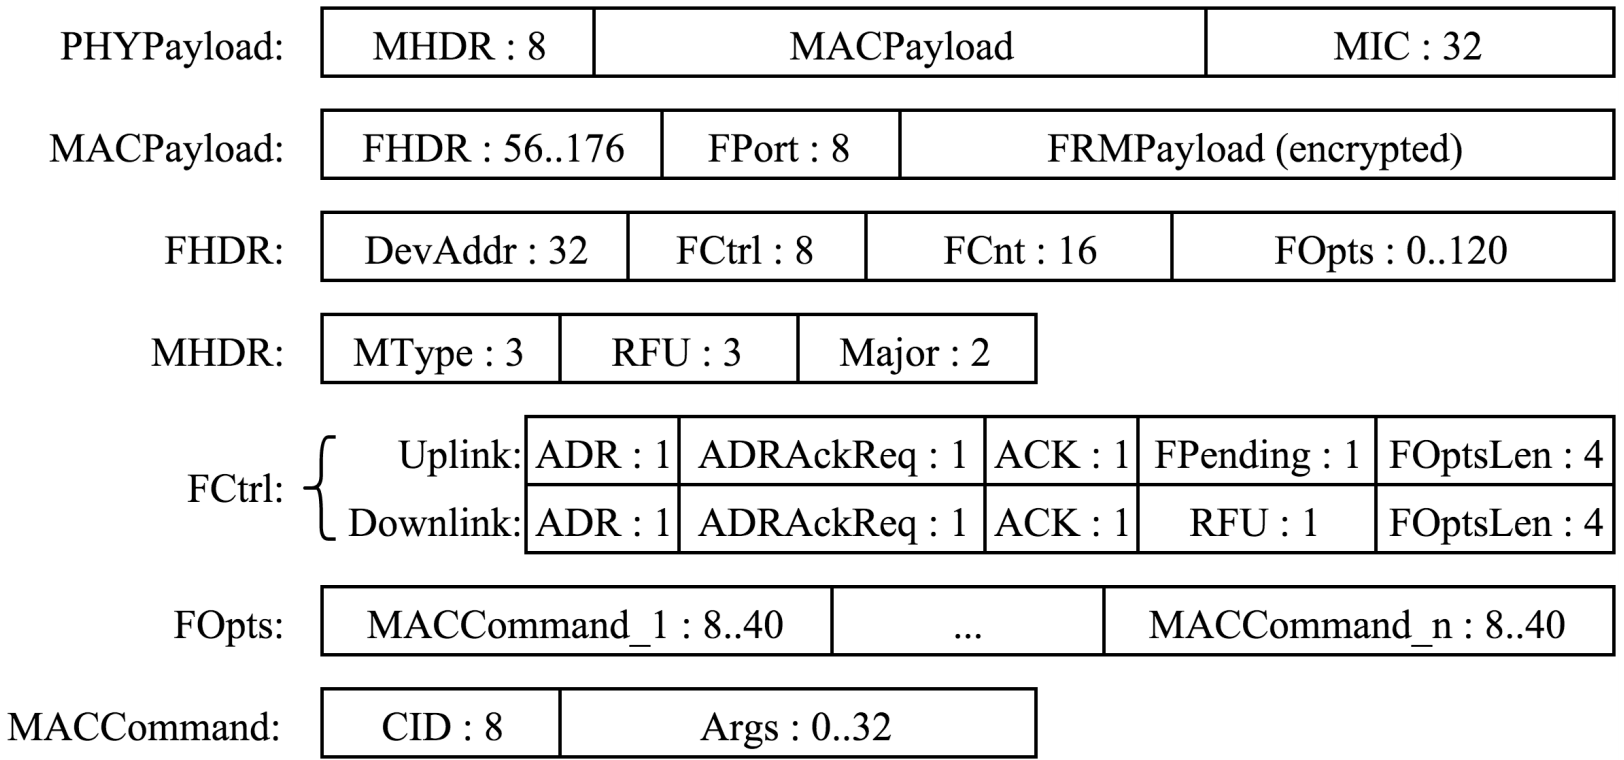
\includegraphics[width=\textwidth]{lorawan_message_format.png} 
\caption[Formato paccchetto LoRaWAN]{Formato paccchetto LoRaWAN}\label{fig:venti}
\end{center}
\end{figure}

Di seguito la descrizione dei campi:
\begin{itemize}                       
\item DevAddr : indirizzo breve del device.
\item FPort : Se il campo frame payload \`e presente, il campo porta deve necessariamente essere presente. Se il valore di FPort \`e pari a zero indica che FRMPayload contiene solo un MAC command ed ogni frame ricevuto con una FPort deve essere processato.
\item FOptsLen : Deve essere pari a zero quando il frame contiene solo un Mac command. 
\item FCnt : Frama counter
\item MIC : codice di integrit\`a del messaggio crittografato, elaborato attraverso i campi MHDR, FHDR, FPort ed il criptato FRMPayload.
\item MType : Tipo di messaggio, indica tra le altre cose se il pacchetto \`e in uplink o downlink ed inoltre se si tratta di un messaggio di conferma. Un acknowledgments \`e richiesto per i messaggi che lo richiedono.
\item Major : LoRaWAN version. Attualmente \`e ammesso solo il valore pari a zero. 
\item ADR / ADRAckReq : controlla il meccanismo di adaptive data rate da parte del network server. 
\item ACK : acknowledges dell'ultimo frame ricevuto. 
\item FPending : indica che il network server ha dati addizionali da spedire, pertanto l'end-device deve necessariamente inviare un ulteriore messaggio per poter aprire una finestra in ricezione (device di classe A).
\item FOptsLen : \`e la lunghezza del campo FOpts in bytes. 
\item FOpts : trasporta i comandi MAC e viene incapsulato all'interno del data frame.
\item CID : Mac command identifier.
\item Args : argomento opzionale del comando.
\item FRMPayload : payload che viene cifrato attraverso algoritmo AES a 128 bit.
\end{itemize}

\section{End-device setup}
Per partecipare ad una rete LoRaWAN, un end-device deve essere attivato. LoRaWAN fornisce due modi per attivare un end-device : Over-The-Air-Activation (OTAA) e Activation By Personalization (ABP). Il processo di attivazione deve fornire le seguenti informazioni all'end-device :
DevAddr or DevEUI: End-device address. Un identificativo a 32 bit composti da sette usati come network identifier ed i restanti 25 usati come indirizzo associato al dispositivo.
\begin{itemize} 
\item AppEUI : Application identifier. Un identificativo globale dell'applicativo nello spazio degli indirizzi definito da IEEE EUI64 che identifica univocamente il proprietario dell'end-device.
\item NwkSKey : Network Session Key. Una chiave usata dal network server a dall'end-device per calcolare e verificare l'integrit\`a del messaggio.
\item AppSKey : Application Session Key. Una chiave usata dal network server e dall'end-device per cifrare e decifrare il campo payload del pacchetto.
\end{itemize}
Per la modalit\`a OTAA esiste una procedura con scambio di messaggi di tipo join-request e join-accept per ogni nuova sessione. Un end-device \`e in grado di ottenere delle nuove chiavi di sessione (NwkSkey e AppSKey) solo dopo aver ricevuto un messaggio di join-accept. 
Per la modalit\`a ABP, invece, le due chiavi di sessione sono direttamente memorizzate nel end-device.



\section{Sicurezza e minacce LoRaWAN}
In LoRaWAN la sicurezza \`e garantita attraverso l'utilizzo di cifratura AES-128 bit e dispone di due strati indipendenti per quanto riguarda la protezione della rete e dell'applicazione.
La chiave AES-128 bit conosciuta come Application Key (App-key) \`e usata per generare due chiavi di sessione che sono Network Session Key (NwkSKey) e Application Session Key (AppSKey). 
NwkSKey \`e condivisa da sia dall'end-device che dal network server per generare e verificare il codice d' integrit\`a del messaggio (MIC). Il MIC assicura l'integrit\`a di ogni messaggio, e crea una specifica signature per ogni messaggio. 
La AppSKey \`e simile alla NwkSKey, ma \`e usata per cifrare e decifrare il payload dei dati applicativi.
LoRaWAN crea un key stream usando NwkSKey, AppSKey, l'up-link e down-link counter associato ai messaggi. Pertanto ogni messaggio viene cifrato attraverso un'operazione di XOR con la corrispondente chiave a partire dal key stream per generare la cifratura del payload. 
Le procedure di join alla rete da parte dell'end-device possono essere OTAA (Over The Air Activation) e ABP (Activation By personalization). La procedura OTAA richiede i parametri DevEUI, AppEUI e AppKey. Un end-device deve seguire la questa procedura ogni volta che si unisce alla rete o perde le le informazioni relative alla chiave di sessione. OTAA \`e descritto come un modo pi\`u sicuro di autenticazione, in quanto, la network session key viene rigenerata ogni qual volta l'end-device si unisce alla rete. Inoltre questo permette il roaming tra differenti reti. L'end-device inizia la procedura OTAA inviando un messaggio di join-request. Il messaggio include i valori di AppEUI, DevEUI ed un nonce (DevNonce) dell'end-device. Il DevNonce \`e un numero random che \`e generato e tracciato dal network-server ed \`e usato per rigettare ogni join request con un nonce invalido. Questo meccanismo serve a prevenire i replay-attack. 
la seconda procedura di unione alla rete da parte dell'end-device \`e ABP. Questa modalit\`a connette direttamente un end-device ad una rete specifica senza che avvenga una join-request ed una accept procedure. In questo caso i valori di device address (DevAddr), NwkSKey and AppSKey sono direttamente memorizzati all'interno della memoria dell'end-device. In questo modo le chiavi non vengono generate e possono essere direttamente usate per cifrare i messaggi. Se le chiavi sono compromesse, tutte le comunicazioni tra end-device, gateway e network server possono essere decifrate da un'entit\`a terza per tutta la vita dell'end-device.
Una delle potenziali vulnerabilit\`a sfrutta la procedura di join in modalit\`a ABP in quanto le chiavi potrebbero essere derivate da informazioni che diventano pubbliche in quanto ottenute tramite tecniche di reverse engineering di un end-device,  ed a questo punto ogni altra comunicazione di qualsiasi device di quel tipo potrebbe essere compromessa. 
La struttura dei pacchetti LoRaWAN non include per i messaggi una signature o una time based data per validare il timestamp del messaggio e questo pu\`o lasciare il fianco scoperto ad attacchi di tipo replay o wormhole. 
Uno dei possibili attacchi consiste nel compromettere l'end-device e la network key. Un attaccante potrebbe compromettere un end-device accedendovi fisicamente estraendo le chiavi. 
Tipicamente un end-device \`e composto da un modulo LoRa radio receiver ed un host microcontrollore (MTU). Il modulo radio comunica con il microcontrollore attraverso un' interfaccia UART o SPI. 
I comandi ed i dati che passano dall'host al modulo radio possono essere intercettati attraverso un hardware esterno in quanto i moduli radio in commercio non supportano una cifratura incorporata.
In questo modo non c'\`e modo di sapere se i comandi o i dati inviati al modulo radio provengono da MTU originale o da un'entit\`a malintenzionata, la quale potendo intercettare lo scambio di dati tra MTU e modulo radio per creare un mock device con le stesse credenziali per manipolare il payload. Per questo motivo, li sviluppatori di applicazioni non devono eseguire operazioni sensibili come l'impostazione delle chiavi di sicurezza per ogni trasmissione di dati perch\`e potrebbero esporre queste informazioni critiche ad entit\`a malintenzionate. Questo tipo di attacco pu\`o essere fatto collegandosi fisicamente all'interfaccia seriale dell'end-device.


L'attacco di tipo radio jamming \`e un problema che affligge molte tecnologie wireless. Un attaccante pu\`o trasmettere un segnale radio molto potente in prossimit\`a del dispositivo, tanto da compromettere la trasmissione radio. Questo tipo di attacco richiede hardware specifico che per\`o \`e possibile trovare in commercio. La modulazione CSS \`e comprovata essere molto robusta alle interferenze ma la coesistenza di pi\`u dispositivi che trasmettono alla stessa frequenza e con lo stesso spreading factor  potrebbero risentire di interferenza. Questo tipo di attacco viene svolto a livello fisico usando componenti commercial-off-the-shelf (COTS) per dispositivi LoRa allo scopo di creare jamming per una rete LoRa. Banalmente usando un microcontrollore Arduino ed modulo LoRa per creare un flood di messaggi LoRa ad una certa frequenza per poter creare una forte interferenza nelle trasmissioni.
Per poter distruggere le trasmissioni LoRa attraverso un COTS hardware basta un investimento di circa 30 euro. Sebbene \`e difficile prevenire questi tipi di attacchi esistono dei workarounds. Innanzi tutto fare il jamming di un intera rete o frequenza pu\`o essere facilmente intercettata in quanto improvvisamente nessun dispositivo nella rete \`e pi\`u in grado di comunicare. Attraverso l'analisi di questo comportamento anomalo gli amministratori di rete possono prendere provvedimenti come ad esempio modificando la frequenza di trasmissione.
La trasmissione LoRa ha un air-time che varia da qualche millisecondo fino a 1.5 secondi in base alla dimensione del payload e spreading factor. Le trasmissioni wireless verso uno specifico device possono essere identificate attraverso il device address pertanto \`e possibile isolare anche un singolo end-device. Una volta che un attaccante riceve i primi byte dell'header che contengono il device address, se questo indirizzo corrisponde con l'indirizzo del device obiettivo un attaccante pu\`o corrompere attraverso un'azione di selective jammer il resto del messaggio prima che arrivi a destinazione. Questo tipo di attacco \`e molto diffuso anche nelle reti WiFi.
Un replay attack consiste nel trasmettere o ripetere una trasmissione valida da parte di un attaccante fingendo di essere il device originale. Lo scopo principale di questo attacco \`e quello di imbrogliare il device usando un messaggio di handshake oppure dati vecchi dalla rete. Per mettere in atto questo tipo di attacco l'attaccante deve conoscere la frequenza di trasmissione ed il canale per effettuare lo sniff dei dati di una trasmissione tra due devices.
In LoRaWAN non \`e possibile decifrare messaggi tra un end-device ed un gateway senza conosce l'AppSKey in quanto l'intero payload \`e cifrato con essa. Inoltre la manomissione dei dati porta al fallimento del controllo del MIC pertanto non \`e possibile farlo senza conoscere la NwkSKey. 
Sebbene un attaccante pu\`o reinvieare un messaggio consecutivamente, usando il frame counter usato nel frame LoRaWAN, questi messaggi possono essere identificati e scartati. Quando un end-device viene attivato o resettato il counter parte da zero e viene incrementato ad ogni invio di messaggio successivo. Se un messaggio \`e ricevuto con un counter inferiore rispetto all'ultimo messaggio inviato esso viene ignorato. Tuttavia, la specifica LoRaWAN gestisce il frame ma 
i contatori sono specificatamente lasciati all'applicazione e allo sviluppatore. Per questo motivo le reti che non tengono traccia del frame counter possono essere vulnerabili per un replay attack. Inoltre questa misura di sicurezza ha conseguenze per lo sviluppo di dispositivi che usano ABP come modalit\`a di join alla rete. Se un malintenzionato \`e in grado di fare un reset del dispositivo il counter ripartir\`a da zero i messaggi che sono stati ottenuti prima facendo sniffing della trasmissione tra gateway ed end-device possono essere reinviati al gateway. Questo tipo di attacco sfrutta vulnerabilit\`a dell'applicazione, ma nel caso di alcuni allarmi anti intrusione, pu\`o essere sfruttato per fare un replay mentre il device sta inviando un messaggio di allert. In alcune reti per contromisura vengono scartati tutti i messaggi finch\`e il frame counter inviato dai messaggi dell'end-device non raggiunge l'ultimo valore di frame counter che il gateway conosce per quello specifico nodo. In questo tipo di applicazioni a causa di questa contromisura in caso di reset o riavvio del dispositivo, le sue trasmissioni non verranno prese in considerazione per un certo periodo di tempo.       
Il wormhole attack pu\`o essere condotto usando due dispositivi un jammer ed uno sniffer. Lo sniffer ha il compito di catturare pacchetti e invia un segnale al jammer per notificare che i messaggi sono stati catturati. Ovviamente i messaggi catturati non arriveranno mai al gateway, pertanto non essendo mai stati validati restano validi. I messaggi catturati possono essere inviati al gateway in un qualsiasi momento a patto che non ne arrivino altri nel frattempo. Se ad esempio un end-device trasmette un importante pacchetto che indica un allarme, questa trasmissione pu\`o essere disturbata dal jammer e i messaggi che sono stati memorizzati prima e che non hanno mai raggiunto il gateway possono essere inviati in modo che l'applicazione non sappia che \`e stato generato un messaggio di allarme. 
Dato che nel protocollo LoRaWAN non c'\`e nessuna informazione relativo al tempo e quindi i messaggi non hanno un timestamp potrebbe essere molto difficile arginare questo tipo di attacco \cite{K24}







\chapter{Standards LPWAN}
In attesa che lo standard 5G si affacci sul mercato, attualmente esiste una pletora di tecnologie che implementano soluzioni LPWAN. 
Le possibili applicazioni dell'ambito IoT e della comunicazione M2M sono innumerevoli, pertanto ogni tecnologia cerca di affermarsi in macro ambiti differenti per cercare di evitare sovrapposizioni. 
Una delle sfide che coinvolger\`a le diverse organizzazioni \`e l'interoperabilit\`a tra tecnologie eterogenee. 

Il raggiungimento degli obiettivi definiti nel manifesto dell'IoT saranno legati alla capacit\`a che avranno le tecnologie di poter scambiare i dati tra loro. 
Molto dipender\`a dalla visione che hanno i big players nel cercare di convergere verso l'utilizzo di standards aperti che favoriscono l'interoperabilit\`a, oppure se cercheranno di imporre degli standards chiusi per consolidare la posizione di mercato.

Tuttavia considerata la vastit\`a degli scenari possibili e dei contesti applicativi \`e impossibile immaginare un solo standard in grado di coprire tutti i casi. 
E' pi\`u probabile che si arriver\`a ad avere uno standard di riferimento in base all'ambito di utilizzo.
Le principali organizzazioni che operano nel settore dell'elettronica e delle telecomunicazioni, come  Institute of Electrical and Electronics Engineers (IEEE), European Telecommunications Standard Institute (ETSI), and The Third Generation Partnership Project (3GPP) propongono ciascuno il proprio standard. 
A questi si aggiungono i consorzi di aziende che operano in partnership per puntare all'affermazione della tecnologia che sponsorizzano, come ad esempio LoRa Alliance, Weightless-Sig e Dash7 Alliance.

Lo scenario attuale \`e caratterizzato da una forte competizione tra tutti i players del mercato. Attualmente non esiste una tecnologia leader in grado di affermarsi, in quanto le varie soluzioni sono complementari tra loro con pregi e difetti per ciascuna. 
In linea di massima la tendenza \`e quella di inseguire gli interessi di investimento dei grossi players dell'industria piuttosto che concentrare congiuntamente gli sforzi per trovare soluzioni comuni a pi\`u ambiti applicativi. 
Considerata la grande vastit\`a di soluzioni possibili, per poter scegliere quale tecnologia adottare bisogna fare valutazioni approfondite sugli aspetti tecnici sul ritorno d'investimento nell'adottare una soluzione piuttosto che un'altra. 
Se l'analisi comparativa venisse fatta analizzando solo gli aspetti di marketing promossi dai vari istituti, aziende o consorzi si potrebbe optare per una qualsiasi soluzione in quanto nessuna \`e dominante rispetto alle altre.
La previsione \`e che con il tempo alcuni standards si affermeranno a discapito di altri, riducendo l'attuale frazionamento del mercato LPWAN. 
Di seguito verranno descritte le principali organizzazioni, gli standard di riferimento e le innovazioni proposte \cite{K2}.

\section{Ieee} 
Institute of Electrical and Electronics Engineers (IEEE) sta concentrando i propri sforzi nell' estendere il range di copertura del segnale e di ottimizzare il consumo energetico per gli standards IEEE 802.15.4 che definisce le LR-WPAN (Low-Rate Wireless Personal Area Network) e IEEE 802.11 che definisce le WLAN (Wireless Local Area network). 
Il lavoro condotto dall' IEEE consiste nel definire un insieme di nuove specifiche per i livelli PHY e MAC dei rispettivi standards.
Due standards LPWAN sono stati proposti come modifiche allo standard di base di IEEE 802.15.4. 
Il primo standard viene identificato con IEEE 802.15.4k conosciuto come Low Energy, Critical Infrastructure Monitoring Networks. 
TG4k \`e la task group che propone 802.15.4k come riferimento per applicazioni low-energy critical infrastructure monitoring (LECIM) che operano nella banda ISM sia SUB-GHz che 2.4 GHz.       
Lo standard IEEE 802.15.4k \`e stato creato in risposta alle problematiche di trasmissione a corto raggio e alta densit\`a del deploy di dispositivi nelle reti mesh LR-WPAN.
Per sopperire a queste criticit\`a sono state implementate delle modifiche al PHY layer adottando le modulazioni DSSS e FSK. Inoltre \`e possibile usare differenti ampiezze di banda dei canali che spaziano nel range da 100KHz a 1 MHz. 
Le modifiche apportate al PHY layer si riflettono anche sul MAC layer.
L'innovazione che riguarda il MAC layer prevede l'adozione del meccanismo CSMA/CA con PCA (PCA) e di ALOHA con PCA. 
PCA (Priority Channel Access) \`e stato introdotto tramite lo standard IEEE 802.15.4k e definisce il concetto di messaggi con priorit\`a. 
Cos\`i come nello standard IEEE 802.15.4, nella variante 802.15.4k viene definita a livello MAC una struttura superframe. La struttura superframe prevede l'utilizzo dei beacons che sono trasmessi ad intervalli periodici dalla base station che indicano l'inizio e la fine della struttura superframe. Gli end-device devono essere sincronizzati con la struttura superframe per poter trasmettere segnale. La struttura superframe suddivide il tempo in slot logici e comprende due periodi. Il primo periodo conosciuto come CAP (Content Access Period) permette alle varie stazioni radio di contendersi l'accesso al canale tramite meccanismo CSMA/CA. Il secondo periodo conosciuto come CFP (Content Free Period) permette alle stazioni radio di spegnere il trasmettitore per poter ottimizzare il consumo energetico entrando in sleep mode. La feature introdotta con 802.15.4k \`e che opzionalmente \`e possibile aggiungere uno slot nel periodo CAP della struttura superframe. 
PCA \`e allocato solo in presenza di un messaggio con priorit\`a che viene generato in occasione di un evento critico. 
Il PAN Coordinator pu\`o decidere di operare in modalit\`a beacon enabled o non beacon enabled. E' possibile adottare una struttura superframe solo nel primo caso, con il conseguente utilizzo di PCA. Nel caso ci fossero pi\`u allocazioni PCA nel superframe, la prima viene messa all'inizio del CAP, mentre le successive sono uniformemente distribuite su tutto il periodo di CAP. La lunghezza dello slot PCA deve essere sufficientemente ampia per trasportare un messaggio con priorit\`a \cite{K7}.
\begin{figure}[h]                      
\begin{center} 
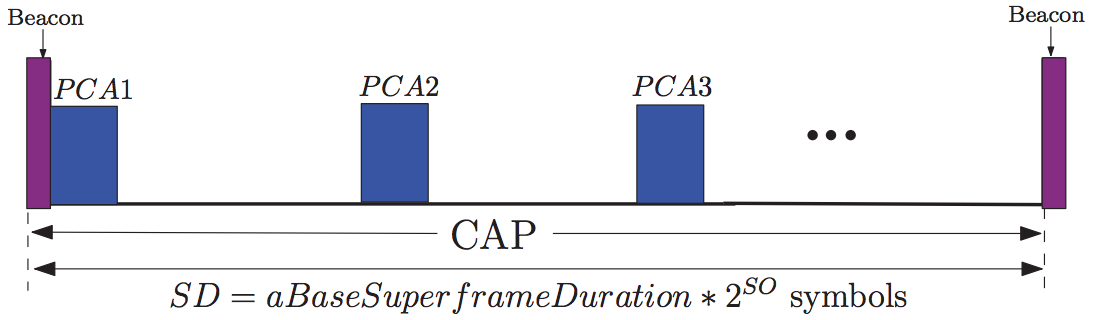
\includegraphics[width=\textwidth]{PCA_Allocation.png}
\caption[PCA allocation]{PCA allocation}\label{fig:quinta}
\end{center}
\end{figure}

Attraverso l'uso di PCA l'end-device e la base station possono adottare meccanismi di priorit\`a per la gestione del traffico di rete introducendo una nuova nozione di QoS. 
Come per le altre tecnologie LPWAN, anche in IEEE 802.15.4k viene adottata una topologia a stella che permette lo scambio di messaggi schedulati e asincroni.
Questo standard \`e stato pensato principalmente per gli scenari applicativi LECIM. 
Lo studio delle performance di questo standard \`e stato fatto per il deploy di un sistema di monitoraggio della qualit\`a dell'aria. E' stata implementata una rete di sensori con topologia a stella con una base station e cinque end-device posizionati in un raggio di 3 Km. L'access point opera nello spettro di frequenza dei 433 MHz. Usando una potenza di segnale pari a 15 dBm il ricevitore pu\`o supportare diverse soglie di sensitivit\`a in base la data rate richiesto raggiungendo valori di -129 dBm, -123 dBm, -110 dBm per i rispettivi data rate di 300 bps, 1.2 kbps e 50 kbps \cite{K8}.

Il livello PHY e MAC di Ingenu \`e compliant allo standard 802.15.4k.
IEEE propone anche lo standard IEEE 802.15.4g che definisce le Low-Rate Wireless Smart Metering Utility Networks. La task force TG4g propose nel 2012 le prime modifiche allo strato fisico dello standard 802.15.4 base in modo da poter supportare le modulazioni FSK (Frequecy Shift Key), OFDMA (Orthogonal Frequency-Division Multiple Access), QPSK (Quadrature Phase Shift Keying) che prevedono diversi data rate nel range tra i 40 kbps e 1 Mbps in base alle diverse regioni. Ad eccezione di una sola banda (attiva solo negli USA), lo strato fisico lavora nella banda ISM Sub-GHz e 2.4 GHz. Il PHY layer \`e stato progettato per il recapito di frame di dimensione fino a 1500 byte per evitare la frammentazione a livello IP dei pacchetti. Le modifiche a livello MAC per essere compliance allo strato fisico vennero gi\`a implementate con lo standard IEEE 802.15.4e per poi essere adottate anche da IEEE 802.15.4g.  
IEEE non si \`e limitata a definire nuovi standard nell'ambito delle LR-WPAN, ma ha proposto anche delle modifiche allo standard 802.11 che definisce le WLAN, permettendo alla tecnologia Wi-Fi di avere un ruolo nel mondo dell'IoT.   
Il task group AH (TGah) il Topic Interest Group (TIG) hanno concentrato i loro sforzi per adattare la tecnologia Wi-Fi ad aumentare raggio di copertura del segnale e diminuire il consumo energetico. 
TGah propone le specifiche per lo standard 802.11ah che permettono a Wi-Fi di operare su long range nella banda ISM Sub-GHZ. 
Rispetto allo standard 802.11ac sono state introdotte nuove features per poter raggiungere coperture fino a 1 chilometro di distanza in ambienti outdoor con data rate fino a 100 kbps. 
Il livello fisico usa la modulazione OFDM che ha un data rate dieci volte pi\`u lento rispetto a 802.11ac .
Il livello MAC dello standard 802.11ah, riduce l'overhead causato dai frames, headers e beacons per ottimizzare il consumo energetico. Inoltre sono supportati migliaia di dispositivi connessi e le collisioni possibili. 
Come accade nella struttura superframe prevista in 802.15.4, gli end-device possono adottare una modalit\`a a risparmio energetico spegnendo il ricevitore radio durante i periodi di inattivit\`a, tuttavia \`e necessaria la sincronizzazione con la base station.
Grazie alle nuove features di ottimizzazione del consumo energetico e aumento del raggio di copertura del segnale lo standard 802.11ah ha apportato notevoli miglioramenti rispetto ad altri standard come 802.11, Bluetooth e Zigbee. Tuttavia esso non \`e ancora del tutto paragonabile alle altre tecnologie che afferiscono all'ambito delle LPWAN, pertanto non \`e ancora considerato come tale. 
Inoltre esistono delle possibili applicazioni che potrebbero necessitare  di un medio data rate con un consumo relativamente basso di energia, che potrebbero far affermare questo standard \cite{K2}.

La fattibilit\`a dell'uso di IEEE 802.15.4ah nell'ambito dell'IoT/M2M \`e stato documentato in \cite{K9}. Gli autori hanno dimostrato che usando la banda dei 900 MHz per le trasmissioni in downlink \`e possibile raggiungere un raggio di 1 Km con un data rate di 100 kbps ed una potenza trasmissiva di 20 dBm. Per le trasmissioni in uplink \`e difficile raggiungere le stesse performance in quanto il client lavora con bassa potenza a 0 dBm e deve abilitare il duty cycle affinch\`e le batterie possono durare anni. 
In questo caso la distanza massima raggiunta \`e di 400 metri. 

\section{Etsi}
European Telecommunications Standard Institute (ETSI) lavora per standardizzare le trasmissione bidirezionali a basso data rate. Lo standard soprannominato Low
Throughput Network (LTN) \`e stato rilasciato nel 2014 con tre gruppi di specifiche, che riguardano i casi d'uso, l'architettura, il protocollo e le interfacce.    
L'obiettivo principale \`e quello di ridurre la radiazione elettromagnetica sfruttando un payload di dimensione ridotta ed un basso data rate. LTN definisce diversi protocolli e interfacce per l'interoperabilit\`a tra end-devices, base station, network server e sistemi di management. Motivati dal fatto che le emergenti reti LPWAN utilizzano sia trasmissioni UNB (come Sigfox e Telensa) che trasmissioni ortogonali a dispersione dello spettro OSSS (come LoRa), lo standard LTN non definisce alcuna restrizione. Questo standard fornisce flessibilit\`a agli operatori, che possono scegliere se adottare la propria soluzione UNB o OSSS nella banda ISM Sub-GHz. La specifica raccomanda di usare BPSK in uplink e GFSK in downlink per le trasmissioni UNB. Per le modulazioni OSSS \`e possibile usare un qualsiasi schema che supporti la bidirezionalit\`a.   
Per quanto riguarda la sicurezza sono previste misure per la cifratura dei dati e metodi di autenticazione. Diversi providers come Telensa, Sigfox e Semtech sono attivamente coinvolti con ETSI per standardizzare le proprie tecnologie.

\section{3GPP}
The Third Generation Partnership Project (3GPP) si pone come obiettivo di indirizzare il mercato dell'IoT/M2M verso le reti cellulari puntando all'evoluzione delle tecnologie esistenti verso una riduzione dei costi e della complessit\`a, miglioramento del segnale e della penetrazione ed ottimizzazione del consumo energetico. 
Le soluzioni proposte da questo organismo operano tutte in bande sottoposte a licenza come Long Term Evolution (LTE) enhancements for Machine Type Communications (eMTC), Extended Coverage GSM (EC-GSM), and Narrow-Band IoT (NB-IoT) e si differenziano tra loro per diversa copertura, data rate, consumo energetico. 
L'obiettivo comune di tutte queste tecnologie \`e di massimizzare il riuso delle attuali infrastrutture esistenti e lo spettro sottoposto a licenza gi\`a delle reti cellulari. 
LTE enhancements for Machine Type Communications (eMTC) \`e stato progettato in quanto lo standard LTE non si adatta alle esigenze del mondo IoT a causa dell'elevato bit rate e consumo energetico. Per ridurre il costo, pur rimanendo compliance ai requisiti LTE, 3GPP ha provveduto a diminuire il picco di data rate ammissibile dalla categoria LTE 1 alla categoria LTE 0 fino alla categoria LTE M passando per diversi livelli del processo evolutivo. In questo modo la riduzione dei costi \`e raggiunta supportando operazioni half duplex (trasmissione bidirezionale alternata) nella categoria 0. Questa scelta ha come effetto di ridurre la complessit\`a del modem e del design dell'antenna.

Il passaggio dalla categoria 0 alla categoria 1 (conosciuta come eMTC) ha comportato una drastica diminuzione dell'ampiezza di banda disponibile in ricezione passando da 20 MHz a 1.4 MHz, che in combinazione con la riduzione della potenza trasmissiva ha portato benefici in termini di costi e consumo energetico. Per aumentare la durata delle batterie, 3GPP adotta due tecniche chiamate Power SAving Mode (PSM) e extended Discontinuous Reception (eDRx). 
Queste tecniche permettono all'end-device di abilitare la sleep mode per diverse ore o anche giorni senza perdere la registrazione alla rete. Inoltre l'end-device evita di monitorare il canale in downlink per prolungati periodi per risparmiare energia. 


Un altro standard proposto da 3GPP \`e EC-GSM. Mentre il Global System for Mobile Communications (GSM) sta terminando la sua esistenza in qualche nazione, alcuni operatori di reti mobile (MNOs) potrebbero prolungare la sua operativit\`a in alcuni mercati. In base a queste assunzioni, 3GPP propone lo standard extended coverage GSM (EC-GSM) con l'obiettivo di usare trasmissioni con potenza di segnale a +20dB nella banda Sub-GHz per una migliore penetrazione negli ambienti indoor. 
Il link budget opera nel range di 154-164 dBm ed \`e fortemente legato alla potenza trasmissiva. 
Con un solo aggiornamento software delle reti GSM, lo spettro del sistema legacy GPRS pu\`o comprimere i nuovi canali logici definiti per i dispositivi EC-GSM. 
EC-GSM sfrutta trasmissioni ripetitive e tecniche di elaborazione del segnale per migliorare la copertura e la capacit\`a dei sistemi GPRS. 
A livello fisico vengono adottate due tecniche di modulazione, la  Gaussian Minimum Shift Keying (GMSK) e la  8-ary Phase Shift Keying (8PSK)  che forniscono picchi di data rate fino a 240 kbps.
Questo standard \`e stato rilasciato nel 2016 ed ha annunciato di poter supportare 50 mila dispositivi per singola base station. 
Sempre nel 2016 fu lanciata un'altra tecnologia 3GPP conosciuta come NB-IoT. NB-IoT \`e stata progettata per effere totalmente compliance ai requisiti delle LPWAN.
NB-IoT non \`e compatibile con 3G ma pu\`o coesistere con GSM, GPRS ed LTE e pu\`o essere supportato dalle attuali infrastrutture LTE con un semplice aggiornamento software. 
Questo tipo di trasmissione pu\`o esistere all'interno di un singolo canale GSM di 200 KHz, all'interno di un singolo LTE physical resource block (PRB) di 180 kHz o all'interno di un canale di guardia LTE.
Se confrontato con eMTC, NB-IoT riduce il costo del consumo energetico riducendo la bandwidth ed il data rate in quanto necessita solo di 180 KHz. 
Inoltre semplifica il design del protocollo ed il supporto alla mobilit\`a. Questa tecnologia dispone di un link budget di 164 dBm e pu\`o connettere contemporaneamente fino a 50 mila device per cella con la capacit\`a di aumentare la scalabilit\`a aggiungendo pi\`u canali. 
A livello fisico si utilizza Frequency Division Multiple Access (FDMA) per le trasmissioni in uplink e Orthogonal FDMA (OFDMA) in downlink [15]. 
Il data rate \`e limitato a 250 kbps per le trasmissioni multi tono in downlink e 20 kbps per le trasmissioni singolo tono in uplink. Secondo alcuni studi la tecnologia NB-IoT pu\`o raggiungere una durata delle batterie di 10 anni quando trasmette 200 byte al giorno in media.   
La tecnologia NB-IoT non \`e esente da alcune criticit\`a. Innanzi tutto \`e possibile ricevere acknowledgement solo per la met\`a dei messaggi trasmessi a causa della limitata capacit\`a del canale in downlink. Questo aspetto implica l'impossibilit\`a di sviluppare applicazioni IoT che necessitano della convalida della ricezione di tutti i messaggi trasmessi. L'implementazione di un meccanismo che renda pi\`u affidabile la trasmissione fa aumentare la complessit\`a dell'applicazione ed il consumo energetico.  Un altro aspetto critico \`e l'utilizzo del packet aggregation, che consiste nell'unire pi\`u pacchetti in uno solo pi\`u grande al costo di aumentare il delay di trasmissione. Questa tecnica, per il design di alcune applicazioni, pu\`o rappresentare un limite. 
NB-Iot pu\`o risentire quando opera in contesti in cui c'\`e un'elevata presenza di traffico dati/voce, in quanto opera una riallocazione dinamica dello spettro per alleggerire la congestione con ripercussioni sulle performance. 
Quando un end-device viene messo in produzione la sua stima di vita \`e di 10/20 anni, il che rappresenta un ordine di grandezza nettamente superiore se paragonato al ciclo di vita dei telefoni cellulari che \`e di circa 2 anni. 
Una delle maggiori criticit\`a che affligge il mondo delle reti cellulari \`e che quando si affaccia una nuova generazione si pongono questioni in merito al mantenimento delle reti legacy, come ad esempio \`e accaduto con l'arrivo del 4G che ha messo in discussione l'esistenza del GSM per poter recuperare lo spettro. Questo punto potrebbe bloccare gli utenti finali che non riuscirebbero ad avere un rientro dell'investimento economico per poter adeguare gli end-devices ai nuovi standard.

\section{Ietf}
IETF (Internet Engineering Task Force) \`e un organismo internazionale che nell'ambito dell'ecosistema LPWAN, ha l'obiettivo di favorire l'interoperabilit\`a nella moltitudine di tecnologie proprietarie, proponendo uno standard che permetta la comunicazione tra dispositivi a basso consumo energetico basata su protocollo IP.
La soluzione proposta da IETF consiste in uno stack basato su IPv6 progettato per lo standard 802.15.4 chiamato 6LowPAN. 
Tuttavia, 6LowPAN \`e stato pensato per poter funzionare nell'ambito delle LR-WPAN che sono caratterizzate, rispetto a LPWAN, da data rate pi\`u elevato, payload di dimensioni maggiori ed un raggio di copertura di media distanza. 
Considerato che i requisiti che caratterizzano le LPWAN sono differenti, si pongono delle sfide per adattare lo standard 6LowPAN alle nuove esigenze. 
Il primo aspetto da considerare \`e che le tecnologie LPWAN sono eterogenee, pertanto ognuna elabora i dati con formati differenti e possiede MAC e PHY layers diversi. 
In secondo luogo va considerato che molte tecnologie operano nella banda ISM, che sono sottoposte a vari vincoli sul massimo data rate, time-on-air, frequenza di trasmissione in base alle normative nazionali. 
Infine buona parte delle tecnologie LPWAN sono caratterizzate da forte asimmetria tra le comunicazioni in downlink e uplink, tipicamente limitando le trasmissioni in downlink. 
Ne consegue che lo stack IP dovrebbe essere abbastanza leggero e flessibile per soddisfare tutti i requisiti e le limitazioni dei livelli sottostanti. 
Sfortunatamente, questi aspetti non sono stati presi in considerazione quando l'IETF ha lavorato allo standard.
Il gruppo di lavoro IETF che sta lavorando ad uno standard basato su stack IPv6 adatto all'ambito LPWAN si \`e formalmente costituito nell'Aprile 2016. 
L'obiettivo \`e quello di fornire connettivit\`a ed interoperabilit\`a a dispositivi appartenenti a tecnologie eterogenee mediante stack IPv6 mantenendo la scalabilit\`a delle infrastrutture. 
Esistono problematiche di natura tecnologica che devono essere affrontare affinch\`e si possa davvero poter fare interoperare i dispositivi tra loro tramite uno stack IPv6.
Le tecnologie LPWAN hanno un payload limitato dei pacchetti, pertanto l'header deve essere adattato alle dimensioni ridotte.
I pacchetti IPv6 potrebbero essere di dimensioni maggiori rispetto al pacchetto di livello MAC, pertanto per poter essere incapsulati andrebbero frammentati e riassemblati. 
Tuttavia molte tecnologie LPWAN non supportano nativamente la frammentazione dei pacchetti a livello MAC, quindi questo processo andrebbe interamente definito. 
Per poter gestire, amministrare e monitorare tutte le componenti di un'infrastruttura LPWAN quali gli end-device, base station, applicazioni, servers \`e necessario che venga definito un protocollo specifico (come SNMP nelle reti LAN) di segnalazione poco complesso che possa integrarsi ed interagire con il livello MAC. 					
I requisiti di sicurezza, integrit\`a dei dati e privacy devono essere necessariamente preservati specialmente in relazione al fatto che le tecnologie LPWAN adoperano trasmissioni radio.
Per rendere il processo legato alla crittografia meno complesso da gestire per i dispositivi con scarse capacit\`a computazionali, spesso si usano tecniche di crittografia con chiavi simmetriche che vengono condivise tra il dispositivo e la rete. Questo fattore potrebbe diventare un aspetto critico dal punto di vista della sicurezza ed andrebbero studiate soluzioni pi\`u robuste \cite{K2}.

\section{LoRa Alliance}
Semtech \`e la societ\`a francese che ha sviluppato il protocollo LoRa e detiene i diritti sulle specifiche dello strato fisico dello stack. Le societ\`a terze che volessero produrre dei dispositivi LoRa compliance devono pagare delle royalties a Semtech per acquisire le licenze. 
Le caratteristiche dei livelli superiori, nonch\`e l'architettura del sistema sono definite tramite specifiche LoRaWAN rilasciate nel Luglio 2015 e gestite dalla LoRa Alliance, un consorzio che raggruppa diversi operatori del settore.  

\section{Weigthless-Sig}
Weigthless Special Interest Group \cite{K10} 
 propone tre standard LPWAN aperti, ognuno dei quali fornisce differenti features, range e consumi energetici. Questi standard operano sia nello spettro ISM che in quello con sottoposto a licenza.  	
Weigthless-W ha un'ottima propagazione del segnale in quanto sfrutta il white space (canali di guardia) dello spettro usato  dalle trasmissioni televisive. Questa tecnologia supporta diverse modulazioni quali la 16-Quadrature Amplitude Modulation (16- QAM) e la Differential-BPSK (DBPSK), nonch\`e un ampio range di spreading factors. 
In base al link budget utilizzato possono essere trasmessi pacchetti con data rate tra 1 Kbps e 10 Mbps. Gli end-device comunicano con la base station utilizzando trasmissioni narrow band. Questa tecnologia ha un inconveniente, dovuto al fatto che il white space dello spettro usato dalle trasmissioni televisive pu\`o essere utilizzato solo in alcune nazioni. Nelle nazioni in cui non \`e possibile sfruttare il white space vengono usati altri due standards che operano nella banda ISM che \`e globalmente riconosciuta.  
Weigthless-N \`e uno standard che utilizza trasmissioni UNB unidirezionali in uplink e a differenza degli standard WEIGHTLESS riesce ad avere una migliore efficienza energetica e minori costi di implementazione del dispositivo. La modulazione usata \`e DBPSK nella banda Sub-GHz. Il numero di scenari applicativi possibili \`e limitato dal fatto che sono ammissibili solo trasmissioni unidirezionali.   
Weigthless-P utilizza due modalit\`a di accesso al canale a livello fisico. La prima modalit\`a usa la modulazione GMSK, mentre la seconda usa QPSK, perci\`o gli end-device possono essere prodotti senza integrare un chipset proprietario. I canali narrow band hanno una bandwidth di 12.5 KHz ed operano nello spettro ISM, in cui raggiungono data rates in range che varia tra 0.2 kbps e 100 kbps.
Per supportare in pieno il meccanismo di acknowledgments e le capacit\`a di comunicazioni bidirezionali \`e possibile fare un firmware upgrade over-the-air.       
Tutti gli standards Weigthless utilizzano chiavi simmetriche per la crittografia dell'autenticazione degli end-devices e per l'integrit\`a dei dati.

\section{DASH7}
DASH7 Alliance \`e un consorzio industriale che definisce uno stack di rete completo e verticale per connettivit\`a LPWAN conosciuto come DASH7 Alliance Protocol (D7AP) [19]. 
Originariamente questa tecnologia nello standard ISO/IEC 18000-7 veniva impiegata per dispositivi RFID, per poi evolversi in uno standard che fornisce connettivit\`a a medio raggio per sensori e attuatori.
DASH7 impiega trasmissioni narrow band con modulazioni GFSK nella banda Sub-GHz.   
A confronto con le altre tecnologie LPWAN, DASH7 presenta alcune sostanziali differenze.
Innanzitutto utilizza una topologia di rete ad albero come default e non a stella.
Nella topologia ad albero gli end devices sono collegati ad un duty-cycling sub-controllers (approfondire questo tema) che li collega alla base station che \`e sempre accesa. 
Questo meccanismo di duty cycle aggiunge complessit\`a al design dei layers superiori.   
Il livello MAC di DASH7, impone agli end-device di ascoltare periodicamente il canale per verificare la presenza di eventuali trasmissioni in downlink. Questo meccanismo permette di avere comunicazioni soggette a poca latenza ma al prezzo di un maggiore consumo energetico a causa dell'attivit\`a di ascolto del canale.
Infine, a differenza delle altre tecnologie LPWAN, DASH7 definisce uno stack di rete per intero permettendo alle applicazioni e agli end devices di comunicare tra loro senza dover gestire la complessit\`a dei layers PHY e MAC.
DASH7 implementa il supporto per forward error correction ed usa chiavi simmetriche per la crittografia.

\chapter{Problematiche aperte e sviluppi futuri delle LPWAN}
Uno dei motivi del successo delle reti LPWAN deriva dell'immediatezza con cui \`e possibile sviluppare applicazioni IoT grazie al basso costo dei dispositivi.
Tuttavia bisogna considerare che ogni tecnologia presenta punti di forza e debolezza, pertanto gli operatori di settore stanno lavorando intensamente per apportare innovazioni tecnologiche che possano tradursi in vantaggi competitivi rispetto alla concorrenza.
Dal punto di vista commerciale, stiamo assistendo ad una vera battaglia tra i diversi vendors su pi\`u fronti. 
Da un lato ogni produttore spinge affinch\`e la propria tecnologia si affermi come standard di riferimento quantomeno per un ambito specifico. Sarebbe \`e alquanto fantasioso immaginare che una sola tecnologia possa affermarsi nella moltitudine degli scenari applicativi possibili nel mondo dell'IoT.
Un altro fronte su cui ci sono forti battaglie commerciali riguarda i servizi e le piattaforme a corredo di una tecnologia. Dal punto di vista dell'immediatezza nello sviluppare un'applicazione IoT, a molti utenti finali potrebbe non interessare la complessit\`a di un'infrastruttura, ma quello a cui potrebbero essere interessati \`e l'accesso ai dati tramite una piattaforma facilmente accessibile ed integrabile con altri servizi.  
Dal punto di vista tecnico ci sono ancora molti aspetti che pongono diverse sfide per le tecnologie LPWAN. Di seguito verranno trattate alcune criticit\`a e le sfide verso cui si stanno concentrando gli sforzi. 

\section{Scalabilit\`a della rete}
Le reti LPWAN metteranno in comunicazione milioni di dispositivi che invieranno dati tramite trasmissioni wireless. Molte di queste tecnologie, usano uno spettro condiviso, pertanto l'allocazione delle risorse \`e complessa a causa di molteplici fattori. 
Il primo problema riguarda la densit\`a del numero di dispositivi presenti nella stessa area geografica. Molte tecnologie adottano una topologia a stella, che sebbene ha il vantaggio di ridurre la complessit\`a del deploy ha lo svantaggio di sovraccaricare la base station, mettendola in condizioni di stress. 
Questo problema viene identificato come hot-spot problem. Il numero di dispositivi che possono collegarsi ad una singola base station pu\`o crescere in modo impredicibile e se la densit\`a \`e elevata all'interno di un'area geografica ristretta, la qualit\`a del servizio potrebbe risentirne notevolmente.  
L'interferenza causata da altre tecnologie pu\`o degradare notevolmente le performance delle reti LPWAN. Questo problema \`e maggiormente accentuato per quelle trasmissioni che operano nelle banda ISM dove vi \`e maggiore intasamento. 
Tuttavia bisogna precisare che anche le tecnologie che operano negli spettri di frequenze sottoposti a licenze sono afflitte dal problema della condivisione dello spettro.
Molte tecnologie LPWAN che usano le reti cellulari adoperano trasmissioni su canali narrow band o addirittura ultra narrow band, il che significa che possono subire interferenza dai servizi che operano in broadband come il video e la voce. 
Inoltre molte tecnologie LPWAN usano a livello MAC protocolli come ALOHA o CSMA che degradano molto in termini di qualit\`a di servizio all'aumentare del numero di stazioni radio.
Recenti studi hanno messo in discussione la capacit\`a che hanno alcune tecnologie di poter scalare a livello di aree geografiche cittadine o addirittura nazionali supportando un elevato numero di end devices.
Un gruppo di ricercatori ha messo in evidenza i limiti di scalabilit\`a del protocollo LoRaWAN, stimando che il numero massimo di dispositivi supportato \`e di 120 nodi in 3.8 ettari (380000 mq) \cite{K11}.

La densit\`a prevista in futuro, del numero di dispositivi per metro quadro, in ambiente metropolitano \`e molto pi\`u alta della capacit\`a reale che pu\`o sostenere la tecnologia  LoRaWAN. 
Tuttavia bisogna precisare che le analisi sulla scalabilit\`a sono state fatte usando dei simulatori software, pertanto in contesti reali questi valori potrebbero addirittura peggiorare in quanto potrebbero esistere variabili ambientali che non possono essere simulate.  
Inoltre \`e stato dimostrato che la copertura del segnale LoRa decade in maniera esponenziale all'aumentare del numero di end-devices a causa dell'interferenza causata dai dispositivi \cite{K12}.

Entrambi gli studi \cite{K11} \cite{K12} suggeriscono che per migliorare le perfomance di un'infrastruttura LoRaWAN sarebbe opportuno usare delle base station pi\`u sofisticate, con la capacit\`a di variare alcuni parametri di trasmissione in modo da sfruttare la diversit\`a delle base station al fine di ottenere una scalabilit\`a migliore.
Molte ricerche hanno messo in evidenza i limiti di scalabilit\`a delle tecnologie LPWAN, proponendo alcuni temi che possono essere perseguiti per migliorare il servizio. 
Alcune soluzioni propongono l'uso di diversi canali, opportunistic spectrum access e  and adaptive transmission strategies. 

La tecnica del channel hopping (salto di canale) e la possibilit\`a di usare base station multimodem possono sfruttare la diversit\`a di canali e hardware.
Per poter sopperire al problema delle interferenze causate da altre tecnologie che operano sulla stessa banda, sar\`a necessario adottare delle soluzioni cross-layer che tengano in considerazione le caratteristiche peculiari dei vari pattern di trasmissione.
Inoltre per poter ottenere una adeguata scalabilit\`a delle reti LPWAN, a cui saranno collegati migliaia di dispositivi, sar\`a necessario migliorare il livello MAC di molte tecnologie consentendo l'invio solo di brevi messaggi \cite{K13}.

Nel contesto delle tecnologie LPWAN basate su reti cellulari, qualora il traffico generato dal mondo IoT/M2M dovesse superare o interferire con il traffico voce delle reti legacy, alcuni providers di telefonia potrebbe considerare l'ipotesi di spostare questo traffico sullo spettro non licenziato.
Lo spettro di frequenze, soprattutto nella banda libera da licenza, \`e una risorsa condivisa a che le stazioni radio sfruttano in maniera opportunistica. I dispositivi non accedono in modo coordinato al mezzo trasmissivo e tantomeno vengono implementate strategie eque per la condivisione della risorsa. Gli unici vincoli che regolamentano l'accesso al canale nella banda ISM \`e il meccanismo di duty cycle. 
Tuttavia, considerato l'approccio opportunistico dell'uso dello spettro radio, sono state sviluppate soluzioni come il cognitive software-defined radios (SDR) che possono venire in aiuto quando pi\`u tecnologie hanno bisogno di competere per lo spettro condiviso.
I ricevitori radio sono circuiti elettronici che vengono prodotti per poter demodulare il segnale di uno specifico standard (UMTS, GSM, Wi-Fi, ...) e funzionano tutti secondo il principio per cui grazie ad circuito chiamato demodulatore si riporta il segnale dalla banda traslata in banda base. 
SDR, invece, permette di costruire ricevitori radio con un chip generico programmabile via software che \`e in grado di adattarsi a diversi standard. Grazie a questo dispositivo \`e possibile ricevere e trasmettere diverse forme d'onda per una pluralit\`a di standards. 
Questo \`e possibile grazie al ribaltamento dell'idea di costruire circuiti hardware per uno specifico standard, ma che il ricevitore sia completamente software e quindi programmabile per adattarsi a differenti standard su un chip hardware generico. 
Gli attuali ricevitori funzionano effettuando la demodulazione del segnale portando il segnale dalla banda traslata (f0) alla banda base (attorno allo zero) passando per le medie frequenze. 
Il campionamento del segnale viene fatto sulla banda base in quanto \`e un segnale che ha frequenze basse pertanto \`e molto pi\`u semplice decodificare l'informazione. 
La tecnica di SDR consiste, invece, nell' effettuare il campionamento e conversione direttamente in banda traslata senza trasporto in banda base. Questa operazione \`e molto onerosa, in quanto secondo il teorema del campionamento di  Nyquist-Shannon, affinch\`e si possa ricostruire adeguatamente il segnale, \`e necessario usare una frequenza di campionamento (fc) pari almeno al doppio della frequenza limite superiore dello spettro del segnale (ovvero almeno il doppio della banda). Ad esempio se volessimo demodulare il segnale dello standard Wi-Fi che opera con una portante a 2.4 GHz avremmo circa fc=5 GHz , ovvero occorrerebbe gestire una mole di campioni pari a 5 miliardi al secondo \cite{K14}
Attualmente non esiste una tecnologia in grado di svolgere una elaborazione cos\`i sofisticata, pertanto SDR \`e una soluzione che potr\`a essere considerata in prospettiva per poter essere impiegata efficacemente in ambiti LPWAN dove lo spettro di frequenze viene conteso da diverse tecnologie che creano interferenza vicendevolmente. 
Tuttavia in prospettiva, grazie a SDR, si potranno costruire degli end-device il cui livello fisico potrebbe essere totalmente software e quindi riprogrammabile. Questo aspetto introduce un enorme vantaggio in quanto permetter\`a ad un end-device di adattarsi al contesto usando dinamicamente uno standard differente. 
Il problema della gestione della scalabilit\`a delle reti LPWAN in presenza di deploy con un numero massivo di dispositivi concentrati in aree ad elevata densit\`a che trasmettono in maniera non coordinata, pone diverse sfide sul tema di cercare di mantenere il livello di interferenza basso. 

\section{Interferenze ed attenuazione}
La crescita esponenziale del numero di dispositivi e delle relative trasmissioni radio causer\`a inevitabilmente un elevato livello di interferenza, soprattutto per gli standard che operano nella banda non licenziata ISM. 
Alcuni studi hanno messo in evidenza come il livello di interferenza metter\`a a serio rischio il livello di copertura e sostenibilit\`a delle reti LPWAN.  
La banda ISM offre l'enorme vantaggio di poter trasmettere segnali radio senza dover pagare la licenza di utilizzo dello spettro. In accordo con le regolamentazioni nazionali, che normano l'utilizzo del mezzo trasmissivo condiviso, esistono delle limitazioni sulle modalit\`a di accesso alle frequenze.
L'utilizzo della banda ISM \`e regolamentato in termini di bandwidth, Effective Radiated Power (ERP) e metodo di accesso al canale. 
Per per la banda ISM 868 Mhz, le politiche di accesso al canale, impongono l'implementazione di meccanismi di duty cycling oppure Listen Before Talk (LBT). 
Il duty cycle \`e definito su una finestra temporale, ovvero si considera il tempo massimo accumulabile da un dispositivo per poter trasmettere in tale finestra. 
Per la banda 868 MHz il duty cycle \`e di 1\% e la finestra temporale \`e di 1 ora, pertanto un dispositivo potr\`a occupare il canale al pi\`u 36 secondi (non consecutivi) in un ora. 
Il metodo LBT, invece, obbliga il dispositivo ad ascoltare il canale per un tempo minimo di 5 ms per verificare se \`e gi\`a occupato da altre trasmissioni prima di trasmettere. 
Le trasmissioni possono procedere solo se il canale non \`e impegnato. Inoltre LBT rafforza queste limitazioni imponendo che la singola trasmissione pu\`o durare al pi\`u un secondo e quattro secondi per una sessione di dialogo o una sequenza di polling. 
Il tetto massimo di tempo accumulabile per le trasmissioni \`e di 100 secondi in un ora. 
Molti dispositivi che implementano il metodo LBT possono applicare una tecnica chiamata Adaptive Frequency Agility (AFA) che permette al dispositivo di saltare da un canale ad un altro in modo da accumulare pi\`u tempo per le trasmissioni. 
Infine i dispositivi che usano LBT devono interrompere le trasmissioni e restare spenti minimo 100 ms dopo ogni trasmissione.

Lo spettro di frequenza ISM 868 MHz \`e suddiviso in 3 bande, ognuna delle quali viene destinata per specifici ambiti. La banda pi\`u bassa (863-865 MHz) \`e assegnata ai dispositivi audio wireless, la banda media (865-868 MHz) \`e destinata alla tecnologia RFID mentre la banda pi\`u alta (868-870 MHz) \`e usata per i sistemi di allarme. Ognuna di queste bande viene suddivisa a sua volta in sotto bande che hanno una regolamentazione differente per ogni nazione. 
L'immagine sottostante riepiloga come \`e suddivisa la banda ISM 868 MHz e le modalit\`a d'accesso e le destinazioni d'uso di ogni sotto banda \cite{K15}.


\begin{figure}[h]                      
\begin{center} 
\graphicspath{https://it.overleaf.com/project/5bb23fa816bccf0dedc574b9/file/5bd97720df8a0403a456f942}
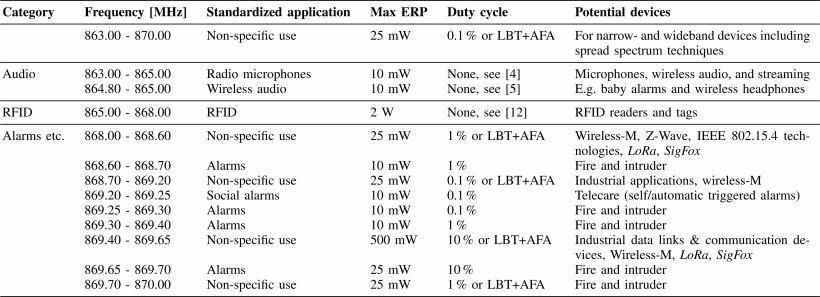
\includegraphics[width=\textwidth]{spettro_868MHz.png}
\caption[Suddivisione spettro 868 MHz]{Suddivisione spettro 868 MHz}\label{fig:sesta}
\end{center}
\end{figure}

LoRa e SigFox, come molte altre tecnologie LPWAN, operano in Europa nello spettro di frequenze che va da 863-870 MHz, che viene destinato per un uso non specifico. 
In modo particolare queste due tecnologie usano lo spettro 868.0-868.6 MHz in uplink e 869.4-869.65 MHz in downlink, ma possono anche usare la rimanente porzione di spettro se necessario. 
In questa banda operano anche le tecnologie a breve raggio LR-WPAN come ZigBee e WirelessHART.
In futuro,l'incremento esponenziale dei dispositivi connessi che usano questa banda di frequenze causer\`a un elevato livello di interferenza tra tecnologie differenti.   		 	 	 
Un gruppo di ricercatori ha analizzato qual'\`e la probabilit\`a di interferenza di segnale in diverse aree urbane. I ricercatori hanno utilizzato un network scanner per analizzare lo spettro 863-870 MHz. 
Le varie rilevazioni sono state fatte per un tempo di due ore ciascuna, in modo da catturare almeno due periodi di duty cycle. Le aree selezionate appartengono a contesti differenti tra loro, al fine di dimostrare come l'interferenza del segnale pu\`o variare in maniera significativa in base allo scenario analizzato.     

\begin{figure}[h]                      
\begin{center} 
\graphicspath{https://it.overleaf.com/project/5bb23fa816bccf0dedc574b9/file/5bd97936df8a0403a456fa5a}
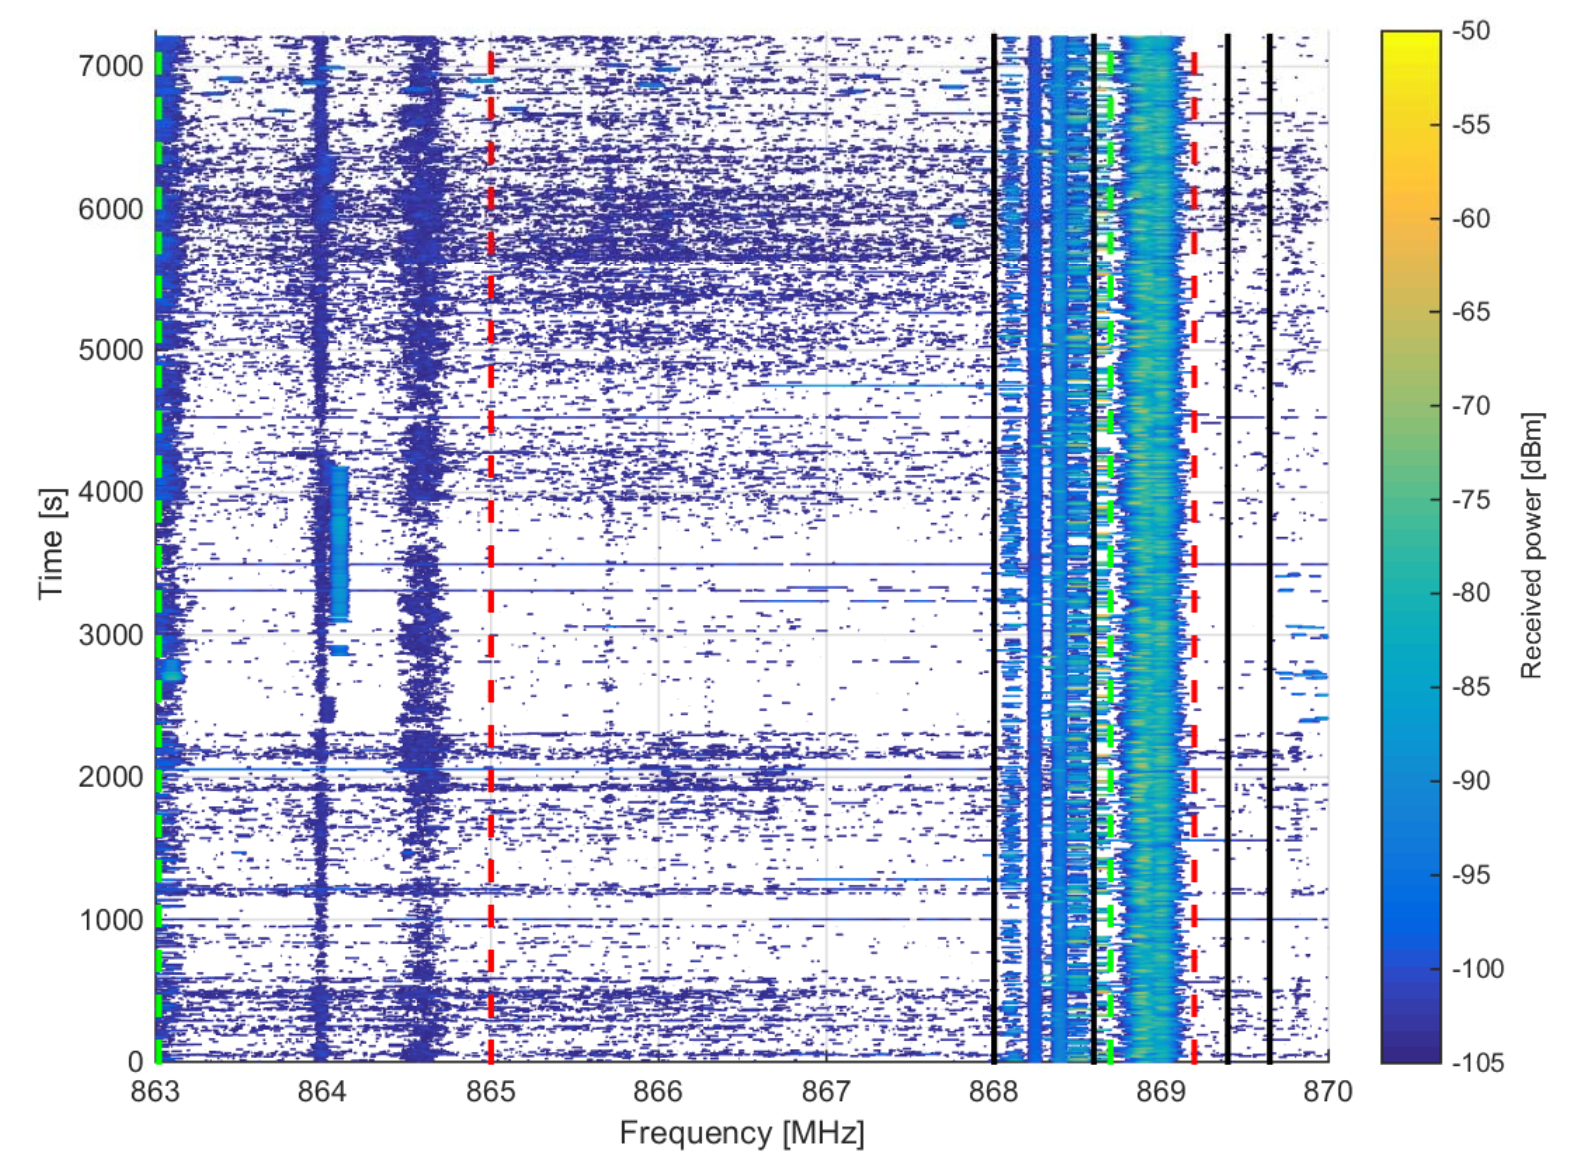
\includegraphics[width=\textwidth]{InterferenceMisurement.png}
\caption[Rilevazione del segnale in un centro commerciale]{Rilevazione del segnale in un centro commerciale}\label{fig:settima}
\end{center}
\end{figure}
La figura 1.7 mostra l'analisi dello spettro 863-870 MHz fatta in un centro commericiale. Il risultato \`e stato esaminato per ogni specifica sotto banda sulla base delle suddivisioni riportate nella tabella precedente. 
La sottobanda pi\`u bassa (863-865 MHz) e quella pi\`u alta (868-870 MHz) sono comprese tra le linee tratteggiate verdi e rosse, mentre le aree comprese tra le linee nere continue sono quelle di maggiore interesse per le trasmissioni di LoRa e SigFox.
La prima considerazione va fatta sulla banda destinata alle applicazioni audio 863-865 MHz. In questa banda non ci sono restrizioni di duty cycle pertanto si evidenzia attivit\`a continuativa. La banda successiva (868.0-868.6 MHz) \`e mandatoria per LoRa e SigFox e la misura effettuata mostra due trasmissioni quasi continue centrate a 868.25 MHz e 868.4 MHz con livelli di potenza pari a -97 dBm e -93 dBm rispettivamente. Considerato che questa banda \`e sottoposta a duty cycle o all'uso di LBT con una trasmissione continua massima di un secondo accumulabile a 100 s in un ora, \`e evidente che ci sono dei dispositivi che violano questa norma, oppure ci sono innumerevoli dispositivi che si sovrappongono nelle trasmissioni. In base a quanto riportato nella tabella riepilogativa della banda ISM 868 MHz i segnali possono essere originati da dispositivi appartenenti allo standard Wireless-M meter oppure da dispositivi in ambito di domotica. 
In uno scenario di questo tipo che potrebbe essere ampiamente ammissibile in un qualsiasi contesto urbano i segnali LoRa e SigFox sono soggetti a forte interferenza.
Gli esperimenti sono stati condotti in diverse aree in contesto urbano e quello che emerge \`e che c'\`e una probabilit\`a di interferenza che varia tra il 22-33\% \cite{K15}.
Un livello di interferenza di questo tipo pu\`o mettere a dura prova la QoS di qualsiasi tecnologia LPWAN operante nella banda ISM, nonostante se vengono impiegate delle modulazioni estremamente robuste che permettono al segnale di sopravvivere anche in presenza di rumore. 
Inoltre sia LoRa che SigFox utilizzano uno schema Aloha per garantire l'accesso al canale che in contrapposizione al metodo LBT non prevede l'ascolto del canale prima della trasmissione facendo precipitare il livello di performance a causa delle molte collisioni. 
Inoltre il deploy di diverse base station posizionate senza alcun coordinamento in aree geografiche ravvicinate, aumenta ulteriormente il livello di interferenza.
Il problema dell'interferenza di segnale non pu\`o essere affrontato solo dal punto di vista tecnologico, in quanto a livello normativo necessita di una forte regolamentazione ma soprattutto di una pianificazione del deploy dei dispositivi. Per ottenere una maggiore affidabilit\`a delle infrastrutture i dispositivi devono schedulare le trasmissioni considerando le variabili tempo, frequenze e spazio. 
Le autorit\`a dovranno proporre delle soluzioni che consentano una condivisione e una cooperazione efficienti tra le diverse tecnologie wireless nelle bande senza licenza. 

\section{Modulazione dinamica}
Per poter ottenere trasmissioni a lungo raggio le tecnologie LPWAN hanno dovuto necessariamente ridurre il data rate. Alcune tecnologie, specialmente quelle che usano modulazione UNB nella banda ISM offrono un basso data rate ed un payload ridotto limitando molto i casi d'uso possibili. 
Per ampliare la scena a casi d'uso che necessitano di maggiore ampiezza di banda la prospettiva sar\`a quella di usare pi\`u schemi di modulazione per singolo device. 
In base al contesto d'uso il dispositivo potr\`a alternare dinamicamente diversi schemi di modulazione migliorando il consumo energetico, il raggio di trasmissione ed il data rate contemporaneamente. 
Per poter ottenere questo risultato sar\`a necessario progettare dispositivi che potranno supportare differenti PHY layer oppure usare SDR al costo di aumentare la complessit\`a ed il costo degli end device. 

\section{Interoperabilit\`a}
Considerato il fatto che il mercato si sta evolvendo verso una competizione sfrenata tra le vari standards LPWAN, \`e lecito pensare che tecnologie differenti potranno coesistere in futuro.
L'interoperabilit\`a tra tecnologie eterogenee \`e un tema cruciale nell'ambito LPWAN soprattutto in relazione alla redditivit\`a. Con poco supporto all'interoperabilit\`a, diventa sempre pi\`u forte la necessit\`a di creare standards.

I maggiori enti di standardizzazione che operano nel settore, quali ETSI, IEEE, 3GPP e IETF si sono posti il problema.  
Per ottenere una piena interoperabilit\`a possono essere esplorate diverse soluzioni. 
Una prima soluzione si basa sull'idea di dotare gli end-device di indirizzo IP in modo che possa essere univocamente identificati e connesso alla rete. Il protocollo IP \`e gi\`a utilizzato per connettere dispositivi che operano in corto raggio usando topologie di rete a mesh. 
L'implementazione dello stack IP su un end device LPWAN non \`e una soluzione perseguibile, in quanto l'intero stack andrebbe semplificato per poter essere eseguito da dispositivi con scarse capacit\`a. Lo standard 6LowPan \`e stato pensato appositamente per questo contesto.
Un altro tipo di soluzione \`e di delegare l'interoperabilit\`a agli apparati di rete che interconnettono una singola rete LPWAN con la rete Internet. 
Questa soluzione \`e adottata attualmente da diverse tecnologie, soprattutto in presenza di topologie a stella in cui la presenza di un gateway e sistemi di backend permettono l'interoperabilit\`a tra reti eterogenee.
Una soluzione alternativa prevede l'utilizzo di sistemi IoT middleware e tecniche di virtualizzazione. 
Un IoT middleware \`e un sistema pensato per interagire con tecnologie di vario tipo utilizzando un'interfaccia specifica per ogni tecnologia. L'obiettivo \`e di raccogliere dati grezzi provenienti da vari end devices e di aggregarli per permettere elaborazioni successive. 
Un IoT middleware si interpone tra gli end devices e il layer applicativo fornendo un livello di astrazione che permette di disaccoppiare le applicazioni dalle specifiche tecnologie.  
Il ruolo svolto \`e quello di consolidare i dati provenienti da diverse sorgenti e di elaborarli per fornire agli utenti finali una base comune per l'accesso a dati aggregati. 

Le piattaforme IoT middleware,  hanno il ruolo di fornire un abstraction layer e si interpongono tra le applicazioni ed i dispositivi permettendo il disaccoppiamento.
In questo modo \`e possibile sviluppare applicazioni generiche che non sono vincolate ad una specifica tecnologia, in quanto \`e compito dell'IoT middleware conoscere la specificit\`a dell'interazione con i dispositivi e di esporre delle API alle applicazioni.
Esistono molte ricerche che hanno affrontato il tema IoT middleware con l'obiettivo di risolvere il problema dell'interoperabilit\`a tra dispositivi eterogenei che operano in diversi domini applicativi. 
Le principali features di un sistema di questo tipo sono: capacit\`a di adattamento, consapevolezza del contesto, scoperta e gestione dei dispositivi, scalabilit\`a, gestione di grandi volumi di dati, privacy, aspetti di sicurezza. 

Un sistema IoT middleware risponde alle seguenti esigenze:
\begin{itemize}                       
\item Difficolt\`a di definire ed imporre uno standard comune tra tutti i diversi tipi di devices.
\item Il middleware agisce da legame tra componenti eterogenee.
\item Le applicazioni di diversi domini richiedono livelli di astrazione / adattamento.
\item Il middleware fornisce le API per il livello fisico e maschera le specificit\`a delle varie tecnologie al livello applicativo.
\end{itemize}
L'architettura del sistema si compone di diversi livelli. La figura 1.8 rappresenta il modello.

\begin{figure}[h]                      
\begin{center} 
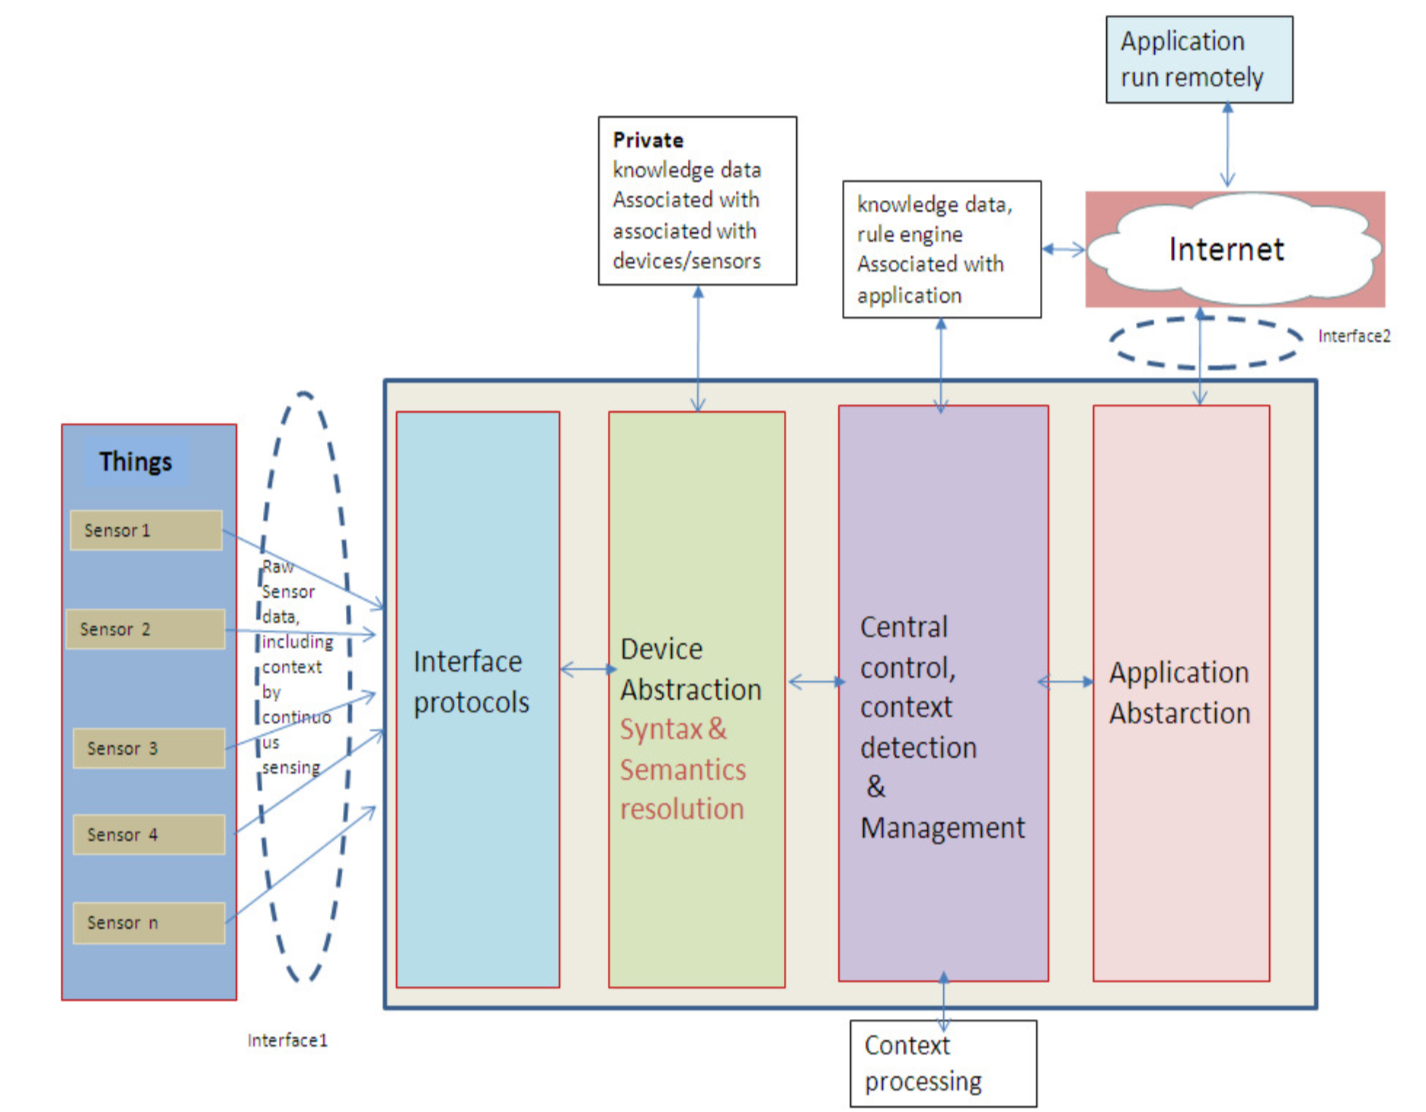
\includegraphics[width=\textwidth]{IoT_Middleware_Architecture.png}
\caption[IoT Middleware Architecture]{IoT Middleware Architecture}\label{fig:ottava}
\end{center}
\end{figure}
Il layer pi\`u importante \`e quello di interfaccia verso il livello fisico, e viene chiamato  interface protocols. 
Il livello di interfaccia \`e in grado di interagire con ogni tecnologia mediante uno specifico protocollo \cite{K16}. 
			
L'interoperabilit\`a una sfida ancora aperta ed in fase di evoluzione. Attualmente non ci sono strumenti in grado di fare stimare con esattezza l'interoperabilit\`a tra diverse tecnologie \cite{K2}.  



\section{Tracciamento e Localizzazione}
Le reti LPWAN forniranno servizi a valore aggiunto a molti ambiti in cui l'aspetto della localizzazione e della tracciabilit\`a delle risorse rappresenta un elemento cruciale. 
Esistono svariati ambiti in cui la localizzazione \`e di interesse strategico, tra cui  la logistica, la gestione delle catene di distribuzione, la tracciabilit\`a dei veicoli nella gestione delle flotte, il monitoraggio di persone o animali e tante altre possibili applicazioni.      
Localizzare in maniera accurata potrebbe non essere banale, soprattutto se non si dispone di tecnologie di localizzazione come i sistemi GPS. 
Tuttavia non \`e sempre possibile l'uso del GPS per rintracciare una risorsa, specialmente se questa \`e collocata in ambienti indoor.  
La localizzazione di dispositivi mobili, \`e un tema ampiamente studiato nelle reti cellulari, dove tipicamente vengono usati metodi che misurano il tempo impiegato da un segnale ad essere trasportato da una sorgente ad una destinazione.
Per poter localizzare in maniera pi\`u o meno accurata una risorsa \`e necessario disporre di un adeguato numero di base station che compongono l'infrastruttura e di tecniche di sincronizzazione.  
Le principali tecniche che possono essere sfruttate sono: beacon location, direction finding e time difference of arrival.     
La tecnica beacon location consiste nel posizionare un ampio numero di semplici ricevitori (beacons) in posizioni strategiche di un'area d'interesse. I beacons possono essere piazzati in diversi punti della citt\`a o lungo le strade. Ogni beacon \`e in ascolto ed intercetta i segnali conosciuti provenienti da dispositivi mobili in transito misurando la forza del segnale ricevuto. In base alla qualit\`a della potenza di segnale che intercorre tra la base station ed il dispositivo \`e possibile stimare la loro distanza. 
Il beacon che riceve il segnale pi\`u forte \`e quello pi\`u vicino al dispositivo. Le coordinate del beacon o la media ponderata del segnale intercettato da pi\`u beacons determina la posizione del dispositivo.
Il vantaggio di questo tipo di tecnica \`e la semplicit\`a e i bassi costi di implementazione, a discapito di una poco accurata stima della localizzazione.
Una tecnica alternativa a quella dei beacons, conosciuta come Angle-Of-Arrival (AOA) consiste nel calcolare l'angolo di ricezione del segnale tra una base station ed un trasmettitore.
Per implementare questa tecnica sono richieste array di antenne direzionali in grado di intercettare segnali provenienti da diverse angolazioni analizzando il beamwidth di ogni singola antenna.
Queste antenne sono abbastanza sofisticate, tuttavia permettono con poche base station posizionate di avere una buona accuratezza della localizzazione. 
Un'altra tecnica, conosciuta come Time Difference of Arrival (TDOA), consiste nel calcolare la differenza in termini di tempo di arrivo di un segnale tra un dispositivo mobile ed una o pi\`u base station. Ogni misurazione TDOA produce una curva iperbolica lungo la quale il cellulare potrebbe mentire, ma grazie all'intersezione di queste curve si pu\`o ottenere la localizzazione. Assumendo che pi\`u base station possono intercettare il segnale di un dispositivo mobile e che ogni base station \`e sincronizzata con un sistema di riferimento, attraverso tecniche di correlazione \`e possibile ottenere la stima accurata.
Il problema di usare tecniche TDOA \`e l'effetto multipath dovuto alla ricezione impredicibile del segnale. Il segnale viene deviato a causa della presenza di ostacoli lungo il cammino.  
Tutte queste tecniche richiedono una accurata sincronizzazione del tempo ed una sufficiente densit\`a di base station. Con una corretta pianificazione del posizionamento delle base station \`e possibile avere una buona copertura a livello di infrastruttura per poter localizzare i vari dispositivi.
In ambito LPWAN la limitata ampiezza di banda dei singoli canali, ed in alcuni casi l'assenza di un path diretto tra base station e dispositivo, pu\`o causare errori nella localizzazione. 
Le tecniche di localizzazione sinora analizzate funzionano bene soprattutto se si usano reti cellulari, tuttavia per le tecnologie LPWAN sarebbe opportuno pensare a soluzioni che non sfruttano solo le propriet\`a del livello fisico ma che sono in grado di combinare altre tecniche di localizzazione \cite{K17}. 

\section{Ottimizzazione del link e adattabilit\`a}
Per poter massimizzare la capacit\`a di una rete LPWAN \`e necessario che ogni collegamento deve essere ottimizzato in termini di consumo energetico e qualit\`a di collegamento. 
Molte tecnologie LPWAN permettono di intervenire su alcuni parametri di connessione in modo da ottenere il miglior trade-off tra data rate, raggio di copertura e time-on-air.   
Metodi di configurazione dinamica dei parametri in funzione delle condizioni ambientali del contesto permettono di migliorare la qualit\`a del servizio. Per molte di queste tecniche \`e fondamentale che ci sia uno scambio di informazioni continuo sulla qualit\`a del link tra il gateway ed end-device. 
Molte tecnologie LPWAN hanno collegamenti asimmetrici tra uplink e downlink, con forti limitazioni soprattutto in downlink. Questa asimmetria ostacola le tecniche di controllo della qualit\`a del collegamento che permettono ai dispositivi di modificare i parametri della trasmissione in modo adattivo, in quanto essendoci trasmissioni in downlink molto limitate le informazioni trasportate vengono destinate ai fini applicativi \cite{K2}.  

\section{Strumenti per il confronto tra differenti tecnologie }
Le tecnologie LPWAN permettono lo sviluppo di una grande vastit\`a di applicazioni in diversi ambiti. 
Considerando il fatto il che molte soluzioni sono tra loro complementari, \`e difficile identificare un metodo che permetta l'analisi di costi e benefici. 

Attualmente, l'adeguatezza di una soluzione rispetto ad un'altra, la scelta di una tecnologia e lo sviluppo del modello di business che pu\`o sostenere un servizio, viene svolto attraverso una profonda analisi del contesto e dei casi d'uso che definiscono i vincoli applicativi.
Per poter realizzare un progetto di una smart city, ad esempio, non \`e assolutamente mandatorio l'utilizzo di una sola tecnologia LPWAN. 
Tuttavia per poter fare il confronto delle performance tra tecnologie differenti non ci sono degli strumenti specifici che operano in ambito delle reti LPWAN in grado di effettuare delle misure su vaste aree geografiche. 

Al momento esistono solo degli studi empirici che permettono di confrontare due tecnologie LPWAN che operano nello stesso contesto.
Considerata l'assenza di tool, testbeds e framework l'unico modo per confrontare le performance \`e quello di effettuare dei test usando dei casi reali. 
Un gruppo di ricercatori ha sviluppato un dispositivo equipaggiato con tante interfacce corrispondenti ciascuna ad una tecnologia differente. Il dispositivo \`e stato collocato in diversi punti al fine di poter raccogliere dati da ogni interfaccia. 
Sulla base dei dati raccolti sono stati fatti i confronti sulle performance in termini di percentuale di dati trasmessi correttamente, ritardo nelle trasmissioni, consumo energetico e raggio di copertura. 
E' importante sottolineare che \`e possibile fare il confronto tra tecnologie LPWAN solo a parit\`a di contesto. Se il contesto cambia i dati ottenuti possono essere molto diversi.
Inoltre sono i requisiti dell'applicazione che vincolano i progettisti ad optare per una soluzione a discapito di un'altra. Ad esempio, quando si progetta un'applicazione bisogna capire se questa \`e delay tolerant o meno \cite{K18}. 

Per le applicazioni event base in cui un attuatore deve reagire con tempestivit\`a al verificarsi di uno specifico evento non \`e possibile adoperare tecnologie che hanno un forte ritardo di trasmissione. Questo tipo di informazioni sono note e fornite dai produttori della tecnologia, tuttavia sapere quali sono le performance effettive in un contesto reale \`e del tutto impredicibile.
L'assenza di strumenti scientifici che possano fornire misure esatte per il confronto delle tecnologie crea barriere in ingresso verso i clienti che vogliono affacciarsi sul mercato delle reti LPWAN.
Sarebbe ottimale che le organizzazioni che governano e gestiscono ambiti specifici mettano a disposizione i risultati ottenuti dall'analisi dei contesti attraverso modelli analitici, in modo da creare aspettative positive in coloro che vogliono investire in applicazioni IoT.

\section{Sicurezza e Privacy}
La sicurezza delle trasmissioni dei dati e la loro integrit\`a \`e un aspetto fondamentale di qualsiasi sistema di comunicazione, soprattutto se wireless. Per poter garantire la sicurezza bisogna utilizzare metodi di autenticazione, sicurezza e privacy assolutamente affidabili.  
Nelle reti cellulari questi metodi sono comprovati essere abbastanza sicuri e vengono sicuramente rafforzati dall'uso delle Subscriber Identity Modules (SIM) che semplificano l'identificazione e l'autenticazione dei dispositivi all'interno della rete.
Le tecnologie LPWAN, a causa dei vincoli relativi ai bassi costi di produzione e del risparmio energetico non dispongono di risorse computazionali e pertanto tendono a semplificare i protocolli di comunicazione e tantomeno utilizzano metodi di autenticazione basati su SIM.
Per ottenere un livello di sicurezza paragonabile a quello delle reti cellulari sono richiesti metodi e protocolli specifici per le tecnologie LPWAN.
Bisogna inoltre considerare il fatto che alcuni dispositivi una volta messi in produzione potrebbero non essere controllati per lunghissimi periodi, pertanto \`e fondamentale ridurre al minimo il rischio di compromissione. Una feature molto importante che supportano alcune tecnologie \`e l'aggiornamento del dispositivi da remoto. Un buco di sicurezza in questa procedura potrebbe compromettere l'intero servizio.   
Esistono delle comprovate vulnerabilit\`a che possono essere sfruttate per colpire alcune tecnologie LPWAN, ad esempio Sigfox non usa nessuna cifratura per il payload dei dati mentre LoRaWAN non usa la cifratura nella procedura di join alla rete. 
Inoltre molte tecnologie LPWAN utilizzano le chiavi simmetriche per la cifratura delle trasmissioni che consiste nell'adottare una sola chiave sia per la base station che per l'end device.
Il tema della sicurezza per le tecnologie LPWAN \`e in fase di miglioramento in quanto non \`e banale coniugare sicurezza e dispositivi a basso consumo energetico.   

\section{Mobilit\`a e Roaming }
Il grande successo delle reti cellulari \`e derivato dal fatto che i dispositivi possono collegarsi alle reti gestite da operatori diversi. Il roaming \`e la capacit\`a dei dispositivi mobili di transitare da una rete ad un'altra, seppur appartenente ad operatori differenti. 
Mentre per alcune tecnologie LPWAN non \`e stato concepito il concetto di roaming in quanto i dispositivi appartengono ad un'unica rete mondiale gestita da un singolo operatore, come ad esempio SigFox, per altre tecnologie non \`e proprio previsto il transito degli end devices da una rete ad un'altra.  
La sfida maggiore sarebbe quella di fornire il roaming senza compromettere il tempo di vita dei dispositivi. Il roaming \`e una feature che molte tecnologie non implementano per evitare impatti significativi sulla vita delle batterie, in quanto per ottenere efficienza energetica si adottano metodi di duty cycle che limitano molto le comunicazioni in downlink. 
Ovviamente questa esigenza diverge con l'implementazione del roaming in cui \`e necessario un meccanismo continuo di sincronizzazione tra un end device e la base station, cos\`i come avviene per le reti cellulari. 
I dati trasmessi in uplink potrebbero essere sfruttati maggiormente per implementare questa feature. Inoltre il processo di transito da una rete ad un'altra pu\`o essere gestito dai sistemi di backend anzich\`e a livello di rete. Le problematiche relative a rendere il processo di roaming pi\`u agile possibile devono ancora essere affrontate, cos\`i come il tema della fatturazione e compartecipazione alle entrate. 
Come avviene per le reti cellulari, anche nelle tecnologie LPWAN, esistono regolamentazioni differenti per quanto riguarda l'accesso al mezzo trasmissivo. Le leggi dei differenti continenti impongono l'utilizzo di frequenze diverse, pertanto \`e pressoch\`e impossibile configurare un un dispositivo in un continente e farlo funzionare in un altro. Il roaming internazionale al momento \`e una sfida alquanto utopistica, perch\`e per realizzarlo i dispositivi dovrebbero essere in grado di identificare l'area geografica in cui operano e di adeguare i parametri per la trasmissione. Questa feature \`e abbastanza complessa da realizzare ed \`e in totale contrapposizione con il principio di produrre end-device poco sofisticati.        
Il tema della mobilit\`a \`e subordinato a quello dell'interoperabilit\`a. Un dispositivo per poter essere considerato mobile deve essere in grado di potersi connettere a diverse reti. 
Fin quando non esisteranno degli standard ufficiali che permetteranno ai dispositivi di tecnologie eterogenee di poter scambiare dati tra loro, tantomeno sar\`a possibile permettere a dispositivi eterogenei di potersi spostare da una rete all'altra \cite{K2}.     	

\section{Service Level Agreements}
L'abilit\`a di poter garantire un certo livello di QoS pu\`o determinare un vantaggio competitivo per i differenti operatori LPWAN.					
Mentre per i providers che operano usando lo spettro di frequenza sottoposto a licenza \`e pi\`u facile garantire un sufficiente livello di QoS, non \`e altrettanto facile quando si opera nello spettro libero da licenza in quanto ci sono numerose restrizioni di legge a cui bisogna adeguarsi. 
Inoltre essendoci il problema dell'interferenza tra diverse tecnologie che operano nella banda ISM \`e ancora meno scontato garantire la QoS. 
Fornire prestazioni di livello carrier su uno spettro condiviso a migliaia di dispositivi che trasmettono in modo non coordinato \`e una sfida importante. E' ragionevole immaginare che i Service Level Agreement (SLA) saranno limitati a causa del fatto che potrebbero essere violati in relazione dell'esistenza di elementi di disturbo non gestibili direttamente dagli operatori di rete.   
Studiare ambienti estremamente rumorosi per sapere se possono essere fornite garanzie di servizio pi\`u rilassato \`e un ambito di ricerca potenziale \cite{K2}.

\section{Coesistenza delle tecnologie LPWAN con altri standards wireless}
Le tecnologie LPWAN sono state progettate per colmare quel gap tecnologico che le reti cellulari e le LR-WPAN non sono in grado di soddisfare. Chiaramente i requisiti alla base della progettazione sono differenti, cos\`i come lo sono i casi d'uso per le applicazioni possibili. 
Tuttavia esistono punti di forza sia nelle reti cellulari che nelle LPWAN. 
In alcuni casi potrebbe essere utile poter beneficiare delle features sia dell'una che dell'altra tecnologia, in modo da ottimizzare le operazioni di alcune applicazioni.					
Esistono dei casi d'uso in cui pi\`u tecnologie possono cooperare l'una con l'altra. 
La specifica ETSI LTN fa una lista di alcuni casi d'uso in cui potrebbe essere utile abbinare le tecnologie cellulari con LPWAN. 
Ad esempio, se la connettivit\`a fornita mediante rete cellulare viene meno, \`e possibile usare un' interfaccia LPWAN come failover per l'invio di soli dati critici. Inoltre il polling continuo che viene fatto per il keep alive nelle reti cellulari potrebbe essere delegato a tecnologia LPWAN per ridurre il consumo energetico.   
Le reti LPWAN possono essere utili per essere di aiuto per la creazione del routing tra due dispositivi che comunicano in una rete cellulare.		
Quando i dispositivi sono fuori la copertura della rete cellulare, \`e necessario costruire un routing multi-hop per raggiungere una base station. La connettivit\`a LPWAN pu\`o essere di supporto per identificare dispositivi in prossimit\`a. Questi casi d'uso possono essere attraenti per applicazioni di pubblica sicurezza in quanto possono garantire maggiore robustezza delle comunicazioni avendo a disposizione pi\`u tecnologie. 
Considerato il fatto che le tecnologie LPWAN sono progettate per trasmettere solo poche informazioni con basso data rate non \`e escluso che in alcuni casi sarebbe utile trasmettere molte informazioni usando un data rate pi\`u elevato e quindi sfruttando un'interfaccia collegata con una rete cellulare \cite{K2}. 







\part{Obiettivo della tesi}
L'elaborato consiste nella progettazione e implementazione sia di un'infrastruttura LoRaWAN, che della relativa piattaforma di data analytics. In modo particolare \`e stata sviluppata tutta la pipeline dalla raccolta dei dati provenienti dai sensori fino all'analisi. 
Nella fattispecie, in questa tesi, la piattaforma di data analytics \`e stata impiegata per analizzare i dati relativi alla QoS della trasmissione radio LoRa.
Lo studio relativo alle performance fornisce informazioni utili su come fare tuning della tecnologia LoRa per la realizzazione di una rete LoRAWAN che sia in grado di operare in ambienti differenti.
Il sistema realizzato pu\`o essere impiegato in diversi contesti applicativi. Tuttavia per la tipologia di sperimentazione effettuata, sono state fatte considerazioni in merito ad applicazioni in ambito di monitoraggio ambientale.
La piattaforma di data analytics permette di raccogliere ed aggregare i dati in modo da rendere pi\`u agile il processo di analisi. 

\chapter{Progettazione}
L'infrastruttura \`e stata progettata seguendo le specifiche LoRaWAN e pu\`o essere impiegata in diverse contesti applicativi in cui vi sia la necessit\`a di raccogliere dati provenienti dall'ambiente e di poterli elaborare successivamente. Uno scenario applicativo tipico di un'infrastruttura di questo tipo \`e il monitoraggio ambientale. A tale scopo l'end device \`e dotato di un sensore di temperatura e umidit\`a per poter mostare un esempio di come sia possibile analizzare in tempo reale dati ambientali.   

\section{Architettura del sistema}
Come da specifiche, l'architettura di un sistema LoRaWAN si compone di: 
\begin{itemize}                       
\item LoRa Node (End Device): Dispositivo in grado di trasmettere dati via LoRa.
\item LoRaWAN Gateway: Dispositivo in grado di ricevere dati da uno o pi\`u end device e di trasmetterli attraverso rete TCP/IP al network server.
\item Network Server: Sistema di back-end che ha la funzione di coordinare le trasmissioni degli end device all'interno della rete LoRaWAN.
\item Application Server: Sistema in grado di elaborare i dati ricevuti e di presentarli in maniera aggregata.
\end{itemize}
In questa tesi \`e stata implementata un'architettura LoRaWAN semplificata, in quanto priva del ruolo di network server. Il motivo deriva dal fatto che \`e stato usato un solo end device quindi le funzionalit\`a offerte dal network server non sono necessarie.  

\begin{figure}[h]                      
\begin{center} 
\fbox{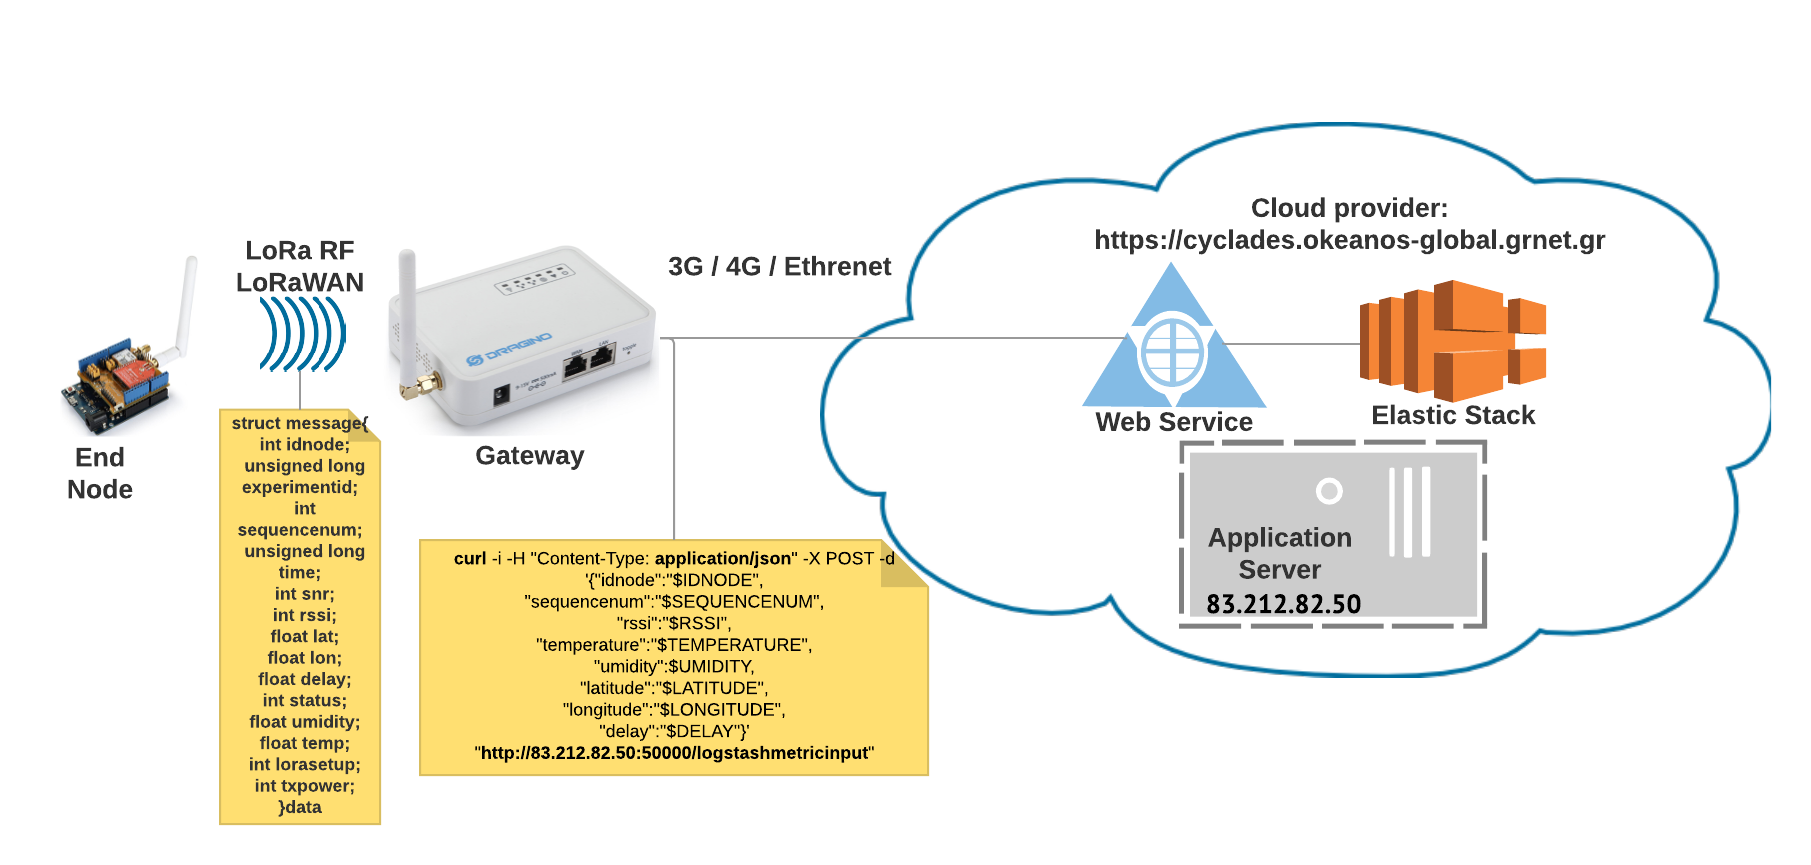
\includegraphics[width=\textwidth]{iotarchitecture.png}}
\caption[Architettura del sistema]{Architettura del sistema}\label{fig:ottava}
\end{center}
\end{figure}


L'infrastruttura del sistema sistema sviluppato si compone dei seguenti nodi:
\begin{itemize}                       
\item LoRa Node (End Device): Scheda di prototipazione in grado di generare e trasmettere segnali LoRa.   
\item LoRaWAN Gateway: Dispositivo in grado di ricevere i dati dall' end device e di trasmetterli attraverso Internet all'application server. Questo nodo non effettua nessuna elaborazione o trasformazione del dato ma si limita ad instradare i pacchetti da rete LoRaWAN a rete TCP/IP.  
\item Application Server: Espone mediante web service un'iterfaccia per la ricezione dei dati provenienti dal nodo gateway. I dati vengono parzialmente elaborati ed inviati all'egine di archiviazione.
\item Search Engine: Sistema di archiviazione basato su paradigma NoSQL in grado di gestire le ricerche per real-time analytics.  
\end{itemize}



 \section{Scelte progettuali}
I tests per la raccolta dei dati ai fini della sperimentazione non sono stati effettuati con tool di simulazione, ma bens\`i attraverso l'uso di dispositivi dotati di ricevitore LoRa in grado di trasmettere e ricevere dati. 
Per questo motivo \`e stato necessario progettare la pipeline in modo da poter raccogliere ed archiviare le metriche relative alla trasmissione.

Le scelte progettuali sono state veicolate da diversi fattori. Gli elementi che hanno guidato la progettazione sono:
\begin{itemize}                       
\item Infrastruttura semplificata: L'architettura del sistema non \`e stata pensata per un servizio in produzione ma per la sperimentazione, pertanto nella progettazione non sono stati valutati meccanismi di alta affidabilit\`a. I nodi dell'infrastruttura non sono ridondati. 
\item Web Service: La scelta di usare un Web Service con il ruolo di middleware deriva da fatto che l'invocazione delle API del search engine usato per archiviare i dati sarebbe stato troppo oneroso e complesso per il LoRa gateway. Il Web Service espone un'interfaccia alla quale  \`e possibile accedere tramite metodo post del protocollo http. 
\item Disponibilit\`a del servizio: Il deploy dell'application server \`e stato fatto presso un'infrastruttura in cloud in modo da disporre di un IP pubblico e di un servizio garantito. 
\item Sicurezza: L'application server espone un web service, pertanto per evitare eventuali compromissioni sono stati adottai meccanismi di protezione mediante firewall.
\item Troubleshooting: Trattandosi di un progetto sperimentale, in alcuni casi si sono manifestate problematiche impredicibili in fase di progettazione. Pertanto, sono stati adottati diversi meccanismi di rilevazione di errori e guasti per permettere la tempestiva correzione dei problemi.
\item Hardware certificato: Si \`e scelto di adoperare un kit certificato per la realizzazione di un'infrastruttura LoraWAN in modo da ridurre i rischi derivanti dall'assemblaggio di componenti. 
\item Disponibilit\`a dei dati: I dati relativi alle metriche sono archiviati ed organizzati in modo da poter essere disponibili per la fase di analisi.
\item Volume dei dati: I dati raccolti dall' end device sono archiviati mediante un database di tipo NoSQL per permettere una maggiore scalabilit\`a anche in previsione di sviluppi futuri.
\item Collaudo del sistema: Il sistema \`e stato ampiamente collaudato prima di iniziare la fase di test vera e propria per evitare che ci fossero valori errati dovuti all'errata progettazione o alla presenza di bugs che potessero invalidare i tests.
\item Consumo energetico: Il sistema \`e stato progettato per la sperimentazione e non per un servizio in produzione, pertanto l'end device \`e stato alimentato tramite un power bank durante la fase test. Non sono state fatte valutazioni in merito al risparmio energetico.
\item Tecnologie consolidate: Il sistema \`e stato realizzato mediante l'uso di tecnologie consolidate per non introdurre ulteriori variabili aleatorie al processo di produzione ed elaborazione del dato. 
\item Identificazione dei test: Per favorire la fase di analisi dei dati allo scopo di valutare i risultati della sperimentazione, ogni esperimento \`e identificato mediante un codice identificativo. 
\item Limitato numero di nodi: Al fine di mantenere semplice il management dell'infrastruttura \`e stato implementato un solo host per il deploy sia dell'application server che del search engine che comunicano tra loro in localhost.   
\item Search Engine: La scelta dell'utilizzo di un search engine basato su database NoSQL di tipo document based, garantisce scalabilit\`a e buone performance di sistema per quanto riguarda l'archiviazione e la ricerca dei dati. In modo particolare la scelta di usare Elasticsearch deriva dal fatto che essendo basato sulla libreria Apache Lucene permette di fare delle interrogazioni su grandi volumi di dati e di gestire i risultati in formato Json.
\end{itemize}
 
\section{Pipeline dai dati}
La pipeline articola in tre fasi: 
\begin{itemize}                       
\item Produzione e trasmissione dei dati: Il dispositivo LoRa end device ha il compito di generare il dato contenente le metriche relative al segnale LoRa. Queste informazioni vengono opportunamente organizzate in una struttura dati che viene incapsulata in un frame LoRa ed inviato al gateway. Il nodo gateway quando riceve un pacchetto proveniente dall'end device provvede ad invocare il web service esposto dall'Application server.
\item Elaborazione ed archiviazione dei dati: L'application server intercetta le informazioni provenienti dal gateway LoRaWAN tramite web service rest. Il servizio compie elaborazioni sul formato dei dati e li organizza per poterli archiviare mediante invocazione delle API messe a disposizione dal search engine. Il search engine \`e basato su paradigma NoSQL e provvede a strutturare e collezionare i dati secondo uno schema document base.
\item Analisi dei dati: Una volta archiviati i dati relativi di un singolo esperimento, questi vengono aggregati sulla base del codice identificativo. I dati vengono estratti ed analizzati in parte attraverso il search engine ed in parte attraverso l'uso di script creati appositamente.   
\end{itemize}
In relazione alla configurazione di ogni test, il pacchetto inviato dall'end device contiene le informazioni relative alla trasmissione LoRa.
L'end device ed il gateway comunicano tramite segnale wireless LoRa. Nel momento in cui il gateway riceve il pacchetto LoRa estrae i dati contenuti nel pacchetto e senza effettuare alcuna manipolazione invoca il web service esposto dall'application server mediante metodo post del protocollo http. Il web service svolge alcune operazioni sui dati ricevuti e li trasferisce al search engine facendo una chiamata tramite interfaccia http esposta.  

\section{Elastisearch}
ElasticSearch \`e un search engine open source divenuto nel tempo molto popolare nell'ambito Big Data, negli ambienti enterprise e nel settore del cloud computing per l'incredibile capacit\`a di ricercare, analizzare e mostrare dati contenuti nei documenti in formato JSON, con interrogazioni che avvengono quasi in tempo reale.
ElasticSearch \`e capace di lavorare con i documenti JSON e si propone come server di ricerca basato su Apache Lucene, una libreria open source per il recupero delle informazioni, le cui caratteristiche peculiari vengono rese disponibili da ElasticSearch agli utenti tramite formato JSON e API per diversi linguaggi.
Questo strumento, a differenza di un normale DMBS transazionale, ha la capacit\`a di poter distribuire i dati su diversi nodi che compongono un cluster Elastic. In questo modo oltre ad aumentare l'alta affidabilit\`a del sistema, si possono ottenere elevate prestazioni nella retrive dei dati.
Ogni dato in Elastic \`e considerato un documento JSON e non ha alcuna relazione con gli altri documenti. Le ricerche possono essere fatte mediante un campo specifico e tramite aggregazione di pi\`u fields.
ElasticSearch \`e uno dei tre layers di Elsatich Stack. I tre layes Elsatich Stack sono cos\`i composti:
\begin{itemize}                       
\item Logstash: Si colloca al livello pi\`u basso ed ha il ruolo di raccogliere dati da diversi tipi di fonti mettendo a disposizione diversi connettori che possono essere invocati per ricevere i dati input. Le fonti dei dati possono essere di diversa natura: logs dei server, dati in formavto csv, json ... Logstash fornisce un'interfaccia per ogni fonte da cui riceve i dati. 
\item Elasticsearch: Rappresenta il motore vero e proprio del sistema. I dati possono essere distribuiti anche su pi\`u istanze di un cluster pertanto quando vengono effettuate le interrogazioni, i risultati vengono estratti mettendo in comunicazione i vari nodi. In Elastic un indice \`e una collezione di documenti che hanno qualcosa in comune. In questo progetto \`e stato definito un indice che memorizza le metriche di un singolo pacchetto LoRa. Logstatsh quando riceve i dati elabora in Elastic un nuovo indice su base giornaliera. Ad ogni invocazione di Logstatsh da parte del gateway viene prodotto un nuovo documento in Elastic che afferisce all'indice di quel giorno. Questo tipo di configurazione viene usata per ottimizzare le ricerche basandosi sulle \textit{time series}.
Per aumentare la scalabilit\`a del sistema un singolo indice pu\`o essere suddiviso in diverse parti chiamate \textit{shards}.
\item Kibana: rappresenta il presentation layer dello stack e mette a dispozione una Dashboard con cui \`e possibile costruire dei grafici in tempo reale sull'andamento di dati contenuti in Elstichsearch.
\end{itemize}

\begin{figure}[h]                      
\begin{center} 
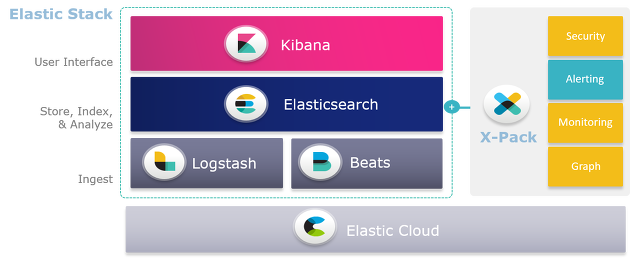
\includegraphics[width=\textwidth]{elasticstack.png}
\caption[Elastic Stack]{Elastic Stack}\label{fig:ventesima}
\end{center}
\end{figure}

\chapter{Implementazione}
In questo capitolo illustrer\`o come sono state implementate le diverse componenti del sistema, descrivendo sia i dispositivi hardware che li strumenti software impiegati per la realizzazione dell'infrastruttura.
 
\section{Dispositivi hardware}
La sperimentazione \`e stata svolta attraverso l'utilizzo di schede di prototipazione dotate di chipset per trasmissione wireless via LoRa.
Nonostante sia possibile costruire da zero sia un LoRa end device che un gateway, si \`e scelto di utilizzare un kit certificato disponibile sul mercato per evitare di aggiungere ulteriori fattori di incertezza alla sperimentazione.
Dopo un'indagine sull'hardware acquistabile, il prodotto migliore \`e risultato essere \textit{Dragino LoRa IoT Kit}. 
Le specifiche sono disponibili a questo link : \url{http://www.dragino.com/products/lora/item/120-lora-iot-kit.html}.
Di seguito la descrizione delle caratteristiche hardware delle singole componenti. \
\\

\textit{LoRa End Device}
\begin{itemize}
    \item Dispositivo: LoRa GPS Shield for Arduino
    \item Documentazione: \url{http://www.dragino.com/products/lora/item/108-lora-gps-shield.html}
    \item Scheda prototipazione: Arduino Uno
    \item LoRa transceiver: SX1276/SX1278 transceiver
    \item LoRa transceiver Spec: 168 dB maximum link budget, +20 dBm - 100 mW constant RF output vs, +14 dBm high efficiency PA, Programmable bit rate up to 300 kbps, High sensitivity: down to -148 dBm, 
    \item GPS transceiver: MTK MT3339
    \item GPS transceiver Spec: Power Acquisition: 25mA,Power Tracking:20mA, Compliant with GPS, SBAS, Programmable bit rate up to 300 kbps, Serial Interfaces UART: Adjustable 4800~115200 bps,Default: 9600bps, Update rate:1Hz (Default), up to10Hz.
\end{itemize}

L'end device LoRa usato nella sperimentazione \`e un Ardunino Uno equipaggiato con un transceiver LoRA SX1276/SX1278 ed un GPS transceiver MTK MT3339. Questo dispositivo dispone delle componenti necessarie alla sperimentazione. Il ricevitore GPS serve per trasmetterre le coordinate geografiche (latitudine, longitudine) del punto esatto in cui si sta effettuando la misurazione. Il LoRa transceiver permette di trasmettere dati e di raccogliere le metriche relative al segnale radio. Il dispositivo \`e dotato di un'antenna per una migliore ricezione del segnale. La figura 8.1 mostra lo shield LoRa usato nella sperimentazione.  

\begin{figure}[h]                      
\begin{center} 
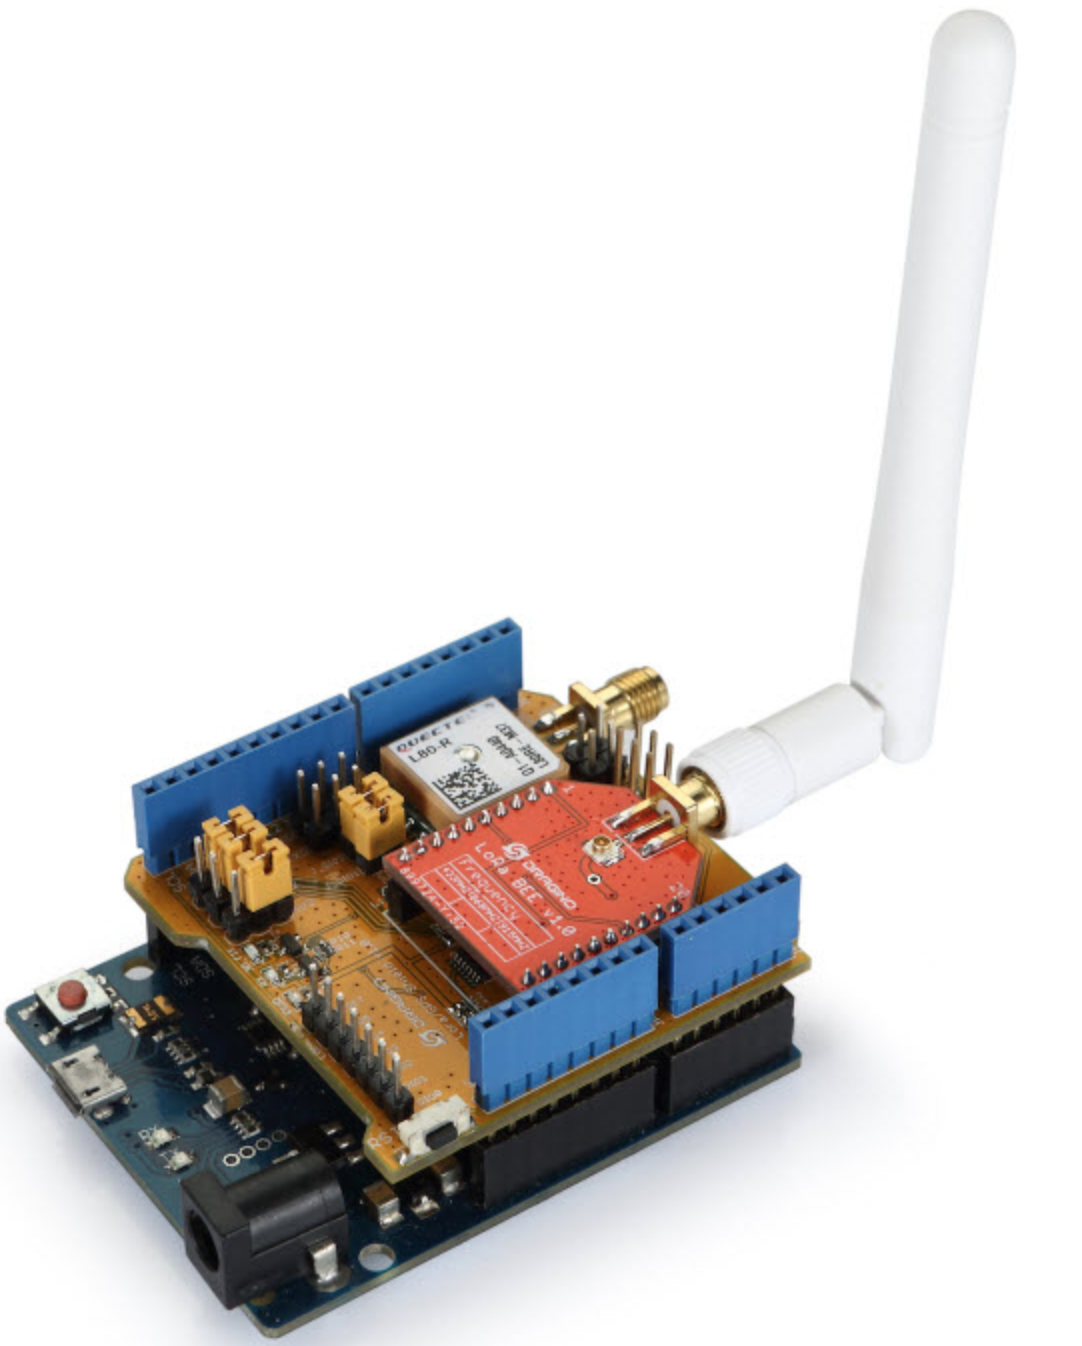
\includegraphics[width=50mm,height=70mm]{LoRa_Shield.png}
\caption[LoRa GPS Shield for Arduino]{LoRa GPS Shield for Arduino}\label{fig:prima}
\end{center}
\end{figure}


\textit{LoRa Gateway}
\begin{itemize}
    \item Dispositivo: LG01-P IoT Gateway featuring LoRa
    \item Documentazione: \url{http://www.dragino.com/products/lora/item/117-lg01-p.html}
    \item Scheda prototipazione: Arduino Yun
    \item MCU: ATMega328P
    \item Flash 32KB, RAM 2KB
    \item LoRa transceiver: SX2176/78 transceiver
    \item LoRa transceiver Spec: 168 dB maximum link budget, +20 dBm - 100 mW constant RF output vs, +14 dBm high efficiency PA, Programmable bit rate up to 300 kbps, High sensitivity: down to -148 dBm, 
    \item Linux Side: Processor 400MHz, 24K MIPS; Flash 16MB ; RAM 64MB
    \item GPS transceiver Spec: Power Acquisition: 25mA,Power Tracking:20mA, Compliant with GPS, SBAS, Programmable bit rate up to 300 kbps, Serial Interfaces UART: Adjustable 4800~115200 bps,Default: 9600bps, Update rate:1Hz (Default), up to10Hz.
\end{itemize}



\begin{figure}[h]                      
\begin{center} 
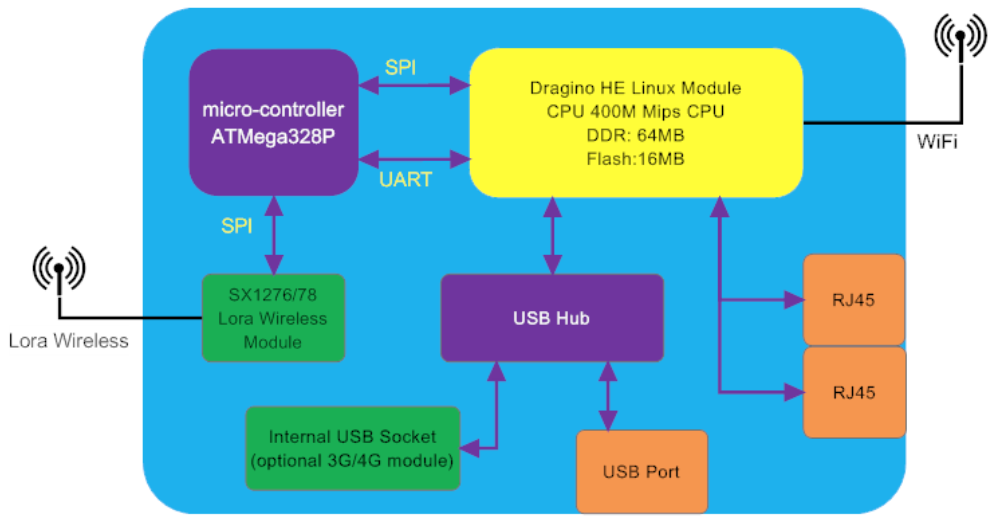
\includegraphics[width=\textwidth]{LoRa_Gateway_Spec.png}
\caption[Architettura del gateway]{Architettura del gateway}\label{fig:prima}
\end{center}
\end{figure}

Il gateway LoRaWAN dispone di capacit\`a computazionali maggiori rispetto all'end device. 
Questo dispositivo permette di interconnettere una rete LoRa con una rete TCP/IP, in quanto \`e dotato di pi\`u interfacce di rete. Il sistema \`e composto di due componenti. Il primo \`e un micro-controllore ATMega328P al quale \`e direttamente collegato via SPI il chipset LoRa. Il secondo \`e micro elaboratore dotato di cpu a 400 MHz, 64 MB di ram e 16 MB di memoria flash. Il sistema operativo installato sul micro elaboratore \`e OpenWrt basato su Linux, che mette a disposizione diverse funzionalit\`a tra cui la gestione delle interfacce di rete WiFi, Ethernet, 3g/UMTS. OpenWrt mette a disposizione un'interfaccia web per la configurazione del sistema. I due componenti sono interconnessi tra loro tramite un bridge. Il vantaggio di un sistema Linux disponibile sul gateway \`e quello di disporre dell'implementazione dell'intero stack TCP/IP e di numerosi tool come curl che permette l'invocazione di url via http. Nella figura 8.2 viene mostrata l'architettura del Gateway LoRaWAN, mentre nella 8.3 il dispositivo.  


\begin{figure}[h]                      
\begin{center} 
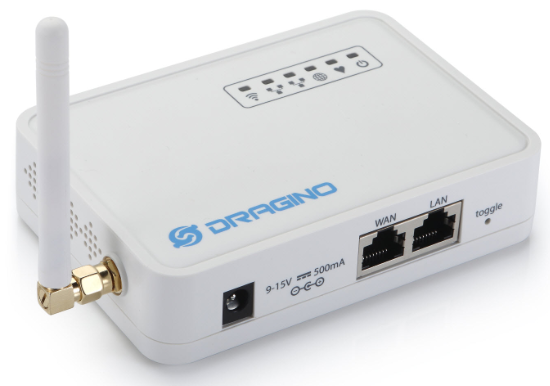
\includegraphics[width=90mm,height=70mm]{LoRa_dragino_GW.png}
\caption[LoRaWAN Gateway]{LoRaWAN Gateway}
\end{center}
\end{figure}

\section{Tecnologie software}
Per lo sviluppo degli sketch delle schede di prototipazione, del web service e degli script per l'analisi dei dati sono stati impiegati diversi linguaggi di programmazione e librerie software. Riporto di seguito un elenco delle tecnologie impiegate nello sviluppo.
\begin{itemize}
    \item C/C++: Svilippo degli sketch, ovvero i programmi che possono essere usati per essere caricati a bordo delle schede Arduino. 
    \item Bash: Shell usata dal micro elaboratore di cui \`e dotato il LoRa gateway. Per l'invocazione del web service tramite curl \`e stato sviluppato uno shell script eseguito dal micro controllore.
    \item Python: Il Web Service \`e stato sviluppato in linguaggio Python versione 2.7 . Questo linguaggio estremamente versatile \`e stato adoperato anche per la creazione degli scripts utilizzati per l'analisi dei dati.
\end{itemize}



\section{Componenti software}
L'architettura del sistema prevede l'utilizzo di una serie di componenti software impiegate per la gestione dei dati. Ogni componente ha un ruolo specifico nella pipeline e permette di gestire il flusso del dato. Per il funzionamento dei microcontrollori Arduino \`e stato necessario sviluppare due appositi sketch. Il web service assolve di ruolo di application server all'interno dell'infrastruttura ed ha il compito di middleware che si interpone tra i dispositivi della rete LoRaWAN ed il sistema search engine che archivia i dati.
I dati vengono  archiviati mediante un database NoSQL che mette a disposizione la funzionalit\`a di search engine chiamato Elasticsearch ed \`e stato impiegato per la raccolta ed analisi dei dati.  

\section{Sketch LoRa End Node}
L'end device ha il compito di raccogliere i dati necessari ai test della sperimentazione. I dati sono memorizzati in una struttura dati di tipo struct

\lstset{language=C,caption={Struttura del messaggio},backgroundcolor=\color{mygray}}
\begin{lstlisting}
struct message{
  int idnode;
  unsigned long experimentid;
  int sequencenum;
  unsigned long time;
  int snr;
  int rssi;
  float lat;
  float lon;
  float delay;
  int status;
  float umidity;
  float temp;
  int lorasetup;
  int txpower;
}data
\end{lstlisting}
Per poter cambiare il setup LoRa durante i test \`e stata implementata una funzione che in base al codice del parametro ricevuto in input effettua le opportune configurazioni.


\lstset{language=C,caption={Funzione configurazione setup LoRa},backgroundcolor=\color{mygray}}
\begin{lstlisting}
void setLoraSetup(){
  // Setup ISM frequency
  rf95.setFrequency(frequency);
  // Setup Power,dBm
  rf95.setTxPower(txpower);
        switch (loraSetup) {
          case 1:
            rf95.setSignalBandwidth(125000);
            rf95.setCodingRate4(5);
            rf95.setSpreadingFactor(7);
            Serial.println("Lora setup 1");
            break;
          case 2:
            rf95.setSignalBandwidth(500000);
            rf95.setCodingRate4(5);
            rf95.setSpreadingFactor(7);
            Serial.println("Lora setup 2");
            break;
          case 3:
            rf95.setSignalBandwidth(31250);
            rf95.setCodingRate4(8);
            rf95.setSpreadingFactor(9);
            Serial.println("Lora setup 3");
            break;
        }
}
\end{lstlisting}

Nel listato 8.3 riporto la porzione di codice con cui vengono gestite l'invio del messaggio e la gestione della risposta. L'invio dei messaggi avviene invocando la funzione \textit{rf95.send()}. Nel listato \`e possibile osservare anche come a seguito del messaggio di risposta del gateway viene calcolato il delay della trasmissione.

\lstset{language=C,caption={Gestione invio dei dati e ricenzione ack dal gateway},backgroundcolor=\color{mygray}}
\begin{lstlisting}
rf95.send((uint8_t *)tx_buf, sizeof(data));
rf95.waitPacketSent();
uint8_t rx_buf[RH_RF95_MAX_MESSAGE_LEN];
  uint8_t len = sizeof(rx_buf);
  if (rf95.waitAvailableTimeout(3000))
  {
    if (rf95.recv(rx_buf, &len))
    {
        memcpy(&datarcv, rx_buf, sizeof(datarcv)); 
        data.delay=(float)(millis()-datarcv.time)/2;
        if (datarcv.status == 1)
        {
         Serial.print("Message from gateway: "); 
         Serial.println(datarcv.status);          
        }      
    }
    else
    {
     Serial.println("recv failed");
    }
\end{lstlisting}



\section{Sketch LoRa Gateway}
Il gateway LoRaWAN non svolge alcuna computazione sui dati in quanto si limita ad instradare i dati ricevuti dal end node verso il web service. Il gateway Dragino \`e composto internamente da un arduiono YUN pertanto \`e possibile eseguire comandi del sottosistema Linux. In questo caso \`e stato sviluppato uno script bash che invoca tramite il comando \textit{curl} il web service passato i dati estratti dal messaggio LoRa in formato json

\lstset{language=C,caption={Ricezione dati da end node ed invocazione shell script},backgroundcolor=\color{mygray}}
\begin{lstlisting}
Process process;
Console.println("Wait for available LoRa Packet: ");
  if (rf95.waitAvailableTimeout(3000))
  {
    uint8_t rx_buf[RH_RF95_MAX_MESSAGE_LEN];
    uint8_t len = sizeof(rx_buf);  
    if (rf95.recv(rx_buf, &len))
    {
        datasize = len;
        memcpy(&data, rx_buf, sizeof(data));
        data.status = 1;     
        memcpy(tx_buf, &data, sizeof(data) );
        rf95.send((uint8_t *)tx_buf, sizeof(data));           
        process.runShellCommand("uploaddatajson.sh");
        process.close();                       
     }
     else
     {
          Console.println("recv failed");
     }
  } 
\end{lstlisting}

Per l'invocazione del web service viene utilizzato il comando \textit{curl}. I dati al web service vengono passati in formato json:
\lstset{language=Bash,caption={Invocazione web service tramite curl e formato dati json},backgroundcolor=\color{mygray}}
\begin{lstlisting}
curl -i -H "Content-Type: application/json" -X POST -d 
'{"idnode":"$IDNODE","sequencenum":"$SEQUENCENUM",
"snr":"$SNR","rssi":"$RSSI",
"temperature":"$TEMPERATURE",
"umidity":$UMIDITY,"latitude":"$LATITUDE",
"longitude":"$LONGITUDE","delay":"$DELAY",
"lorasetup":"$LORASETUP","packetsize":"$PACKETSIZE",
"experimentid":"$EXPID","gw-location":"$GWLOC",
"txpower":"$TXPOW"}' 
"http://83.212.82.50:50000/logstashmetricinput"
\end{lstlisting}

\section{Web Service}
Il web service \`e stato implentato tramite il framework Flask in python. Il suo ruolo \`e quello di intercettare le richieste provenienti dal gateway e di invocare le API di Elasticsearch tramite http per memorizzare i dati. Inoltre ha la funzione di scrivere nel log la distanza geografica che intercorre tra LoRa end node ed il gateway estraendo le rispettive coordinate dal messaggio http ricevuto.  

\lstset{language=Python,caption={Calcolo distanza tra end node e gateway},backgroundcolor=\color{mygray}}
\begin{lstlisting}
dist = mpu.haversine_distance((float(latitude), 
float(longitude)),
(float(gwlat), float(gwlon)))
\end{lstlisting}
\lstset{language=Bash,caption={Invocazione Elasticsearch},backgroundcolor=\color{mygray}}
\begin{lstlisting}
payload = {'sensorId': idnode, 
'sequenceNumber': sequencenum, 
'snr': snr, 'rssi': rssi,
'temperature': temperature, 
'umidity': umidity, 
'node-location': nodelocation,
'time': timestamp, 'delay': delay, 
'lorasetup': lorasetup, 
'packetsize': packetsize,
'experimentid': expid, 
'gw-location': gwlocation, 
'txpower': txpower, 
'throughput': throughput,
'distance': str(dist), 'pdr': str(pdr)}
res = requests.post(url, 
data=json.dumps(payload), headers=head)
\end{lstlisting}


\section{Configurazione Elasticsearch}
La configurazione dello stack \`e abbastanza complessa in quanto bisogna far interagire le diverse componenti. In questa tesi \`e stato implementato uno stack con una singola istanza per ogni layer. Tutte le istanze lavorano su singolo nodo ed in localhost. Nel listato 8.8 viene riportato solo un estratto della definizione dell'indice in Elastic. 

\lstset{language=Bash,caption={Definzione Indice usato in Elastichsearch},backgroundcolor=\color{mygray}}
\begin{lstlisting}
POST _template/sensor_data_template
{
  "index_patterns": ["sensor_data*"],
  "settings": {
      "number_of_replicas": "1",
      "number_of_shards": "5"
  },
    "mappings": {
      "doc": {
        "properties": {
          "sensorId": {
            "type": "keyword",
            "fields": {
              "analyzed": {
                "type": "text"
              }
            }
          },
          "sequenceNumber": {
            "type": "keyword",
            "fields": {
              "analyzed": {
                "type": "text"
              }
            }
          },
          "rssi": {
            "type": "keyword",
            "fields": {
              "analyzed": {
                "type": "integer"
              }
            }
          },
          "temperature": {
            "type": "keyword",
            "fields": {
              "analyzed": {
                "type": "float"
              }
            }
          },
          "umidity": {
            "type": "keyword",
            "fields": {
              "analyzed": {
                "type": "float"
              }
            }
          }
.......
\end{lstlisting}

Per quanto riguarda la configurazione di Logstash ho definito un connettore http che viene invocato dal web service ed a sua volta invoca le API di Elastich per la memorizzazione. Il listato 8.9 mostra la configurazione del connettore http in Logstash:
\lstset{language=Bash,caption={Configurazione connettore http di Logstash ed invocazione indice su base giornaliera},backgroundcolor=\color{mygray}}
\begin{lstlisting}
input {
  http {
    host => "127.0.0.1"
    port => 31311
  }
}
output {
  elasticsearch {
    hosts => ["localhost:9200"]
    index => "sensor_data-%{+YYYY.MM.dd}"
  }
}
\end{lstlisting}

\section{Configurazione di sistema Application Server}
\subsection{Reverse Proxy}
 Il ruolo di reverse proxy \`e stato implementato tramite Nginx \textit{\hyperref[Nginx]{www.nginx.com}}. Il motivo deriva dal fatto che Kibana, il presentation layer di Elastichsearch, fornisce un'iterfaccia a cui \`e possibile accedere senza alcuna auteticazione. Considerando che l'host \`e esposto direttamente ad internet, per ragioni di sicurezza, \`e stato gestita l'autenticazione tramite Nginx. Una volta autenticati il reverse proxy redirige le connessioni http. Il listato 8.10 mostra una parte della configurazione di Nginx per farlo lavorare come Reverse proxy.
\lstset{language=Bash,caption={Configurazione Reverse Proxy di Nginx},backgroundcolor=\color{mygray}}
\begin{lstlisting}
server {
    listen 9000;
    server_name kibanaiot.com;
    auth_basic "Restricted Access";
    auth_basic_user_file /etc/nginx/htpasswd.users;
    location / {
        proxy_pass http://localhost:5601;
        proxy_http_version 1.1;
        proxy_set_header Upgrade $http_upgrade;
        proxy_set_header Connection 'upgrade';
        proxy_set_header Host $host;
        proxy_cache_bypass $http_upgrade;
    }
}
\end{lstlisting}

\subsection{Firewall}
Per ragioni di sicurezza, considerato che l'host \`e esposto direttamente ad Internet, sono state aperte sul solo le porte necessarie al funzionamento del servizio. Il firewall utilizzato \`e Shorewall \textit{\hyperref[Shorewall]{http://shorewall.org/}} che rappresenta un'interfaccia per Iptables ovvero il firewall di default sui sistemi Linux based. Le socket aperte sul firewall sono:
\begin{itemize}                       
\item 9000: Accesso a Kibana tramite Reverse Proxy
\item 50000: Accesso Web Service tramite Flask
\item 22: Accesso via ssh
\end{itemize}

\begin{figure}[h]                      
\begin{center} 
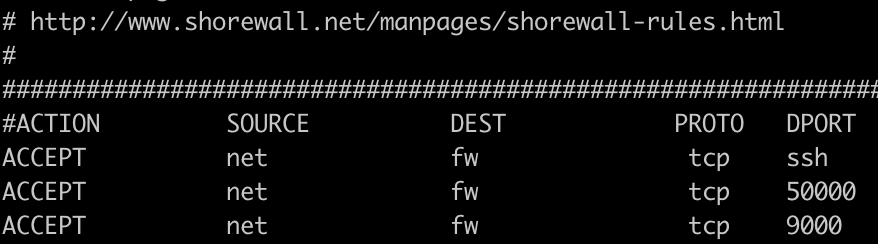
\includegraphics[width=\textwidth]{shorewall.png}
\caption[Configurazione rules Shorewall]{Configurazione rules Shorewall}\label{fig:prima}
\end{center}
\end{figure}

\subsection{Web Service}
Il mircroframework Flask viene eseguito all'interno di un vitualenv Python. L'applicazione \`e gestita mediante demone, pertanto su Centos 7 sono stati implementate le direttive si start e stop per Systemd che permettono la gestione del servizio. Il Web Service sia avvia automaticamente al boot della macchina. 
\lstset{language=Bash,caption={Configurazione Avvio Web Service con Systemd},backgroundcolor=\color{mygray}}
\begin{lstlisting}
[Unit]
Description=uWSGI instance to serve iotnetworkserver
After=network.target
[Service]
User=iotadmin
Group=nginx
WorkingDirectory=/opt/iotnetworkserver
Environment="PATH=/opt/iotnetworkserver/bin"
ExecStart=/opt/iotnetworkserver/bin/uwsgi --socket 
127.0.0.1:3000 --protocol=http -w wsgi  
--wsgi-file iotnetworkserver.py
[Install]
WantedBy=multi-user.target
\end{lstlisting}

\section{Librerie software}
Per ogni tecnologia software sono state impiegate le opportune librerie che hanno permesso lo sviluppo delle singole componenti. 
Di seguito l'elenco delle librerie adoperate.
\begin{itemize}
    \item TinyGPS: Libreria C/C++ usata nello sketch LoRa End Node per la gestione delle coordinate GPS. Attraverso il GPS transceiver \`e possibile conoscere le coordinate di latitudine e longitudine di ogni punto in cui \`e stata fatta la misurazione del segnale LoRa.\
    \url{https://github.com/mikalhart/TinyGPS}
    \item RH\_RF95: Libreria C/C++ usata nello sia nello sketch LoRa End Node che nello sketch LoRa Gateway per la trasmissione dei dati attraverso il transceiver LoRa. Permette di configurare tutti i parametri relativi alla trasmissione tra cui SF, BW, CR. Tra le principali funzionalit\`a vi \`e la possibilit\`a di estrarre i valori di RSSI e SNR. Inoltre fornisce le istruzioni necessarie e le strutture dati per l'invio dei dati.\ 
    \url{https://github.com/PaulStoffregen/RadioHead/blob/master/RH_RF95.h}
    \item TrueRandom: Libreria C/C++ usata nello sketch LoRa End Node per generare un numero random da usare come identificativo dell'esperimento. \ 
    \url{https://github.com/sirleech/TrueRandom}
    \item Process: Libreria C/C++ usata nello sketch LoRa Gateway usata per creare il processo che permette l'esecuizione dello shell cript usato per invocare il web service.
    \item Flask: microframework leggero per Python che permette lo sviluppo di web service Rest. Questo microframework viene eseguito all'interno di un virtual environment ed \`e stato impiegato per lo sviluppo del web service.
    \item Elasticsearch: libreria Python usata negli scripts di analisi dei dati. Offre la funzionalit\`a di interazione con Elasticsearch mediante query. 
    \item Requests: libreria Python usata dal web service per invocare le API di Elasticsearch al fine di archiviare i dati.
    \item Json: libreria Python usata dal web service per strutturare i dati in formato Json compatibili con le API di Elasticsearch. 
\end{itemize}

\chapter{Sperimentazione} 
\section{Obiettivi sperimentazione}
I parametri analizzati permettono di valutare le caratteristiche di una qualsiasi tipo di trasmissione wireless. L'analisi QoS evidenzia quali sono i punti di forza e debolezza di una tecnologia, ma sopratutto permette di identificare quali sono le soglie entro le quali il servizio \`e garantito. 
L'obiettivo della sperimentazione \`e quello di valutare le performance della trasmissione LoRa in termini di:
\begin{itemize}                       
\item Packet Delivery Ratio (PDR): Rapporto in termini percentuali tra numero di pacchetti trasmessi e numero di pacchetti ricevuti.
\item Capacit\`a di trasferimento: Capacit\`a del link di trasmissione espresso in bps.
\item Delay: Tempo impiegato da un pacchetto per essere trasmesso da sorgente a destinazione espresso in millisecondi.
\item Received Signal Strength Indicator (RSSI): Potenza del segnale LoRa captato dal ricevitore LoRa espresso in dBm.
\item Path Loss: Andamento della perdita di segnale al variare della distanza. Differenza tra potenza trasmissiva e potenza di segnale ricevuta in un punto al variare della distanza.
\end{itemize}
Le metriche raccolte vengono analizzate in funzione della variazione della distanza tra ricevitore e trasmettitore LoRa, con lo scopo di individuare le soglie entro cui il trasferimento dei dati \`e garantito. 
La sperimentazione \`e stata svolta in contesti differenti, in modo da confrontare quali sono gli impatti derivanti dalle condizioni ambientali.
Le trasmissioni wireless sono condizionate dalla presenza di ostacoli lungo il percorso, pertanto i tests sono stati condotti sia in area rurale che in ambiente metropolitano.    
Sulla base delle analisi dei dati delle performance \`e possibile fare un confronto tra tecnologie eterogenee al fine di stabilire quale tra quelle esaminate potrebbe soddisfare al meglio i requisiti applicativi in relazione al contesto (al netto dei costi di realizzazione). 
Ad esempio, in ambito metropolitano, esistono pi\`u soluzioni tecnologiche per la trasmissione dati su lungo raggio in quanto \`e forte la presenza delle reti cellulari che garantiscono la copertura di segnale. In ambito LPWAN la tecnologia Nb-IoT rappresenta un'antagonista a LoRa. 
Per poter fare un paragone oggettivo tra le due tecnologie bisogna confrontare le metriche che caratterizzano la trasmissione dati. Le applicazioni si differenziano tra loro in base alla tolleranza al ritardo. Si definiscono applicazioni real time quei servizi in cui non \`e ammesso il ritardo nel recapito dei pacchetti al di sotto di una certa soglia critica. Al contrario, nelle applicazioni delay tollerant la velocit\`a di trasmissione non rappresenta un punto critico, ma sono ammessi ritardi nella consegna dell'informazione. Questa caratteristica rappresenta una forte discriminante quando si valuta quale soluzione adottare. In relazione a questo aspetto \`e stato preso in esame il delay della trasmissione LoRa, per poter stabilire se ad esempio questa tecnologia pu\`o essere impiegata in applicazioni in cui la tempestivit\`a del recapito rappresenta un aspetto cruciale.  
La sperimentazione verte verso la rilevazione delle metriche necessarie a valutare le performance della trasmissione LoRa e di stabilire quali sono gli scenari applicativi migliori in cui poterla adoperare.  
Tra gli obiettivi della sperimentazione non \`e previsto un confronto tra diverse tecnologie, ma i risultai ottenuti possono essere usati come termine di paragone.

La tecnologia LoRa permette il setup di diversi parametri che possono essere combinati tra loro per ottenere le migliori prestazioni in relazione alle condizioni di trasmissione del segnale radio. I parametri relativi alla trasmissione LoRa sono:
\begin{itemize}                       
\item Spreading Factor: Fattore di dispersione della modulazione del segnale LoRa. Determina il numero di chirps che occorrono per rappresentare un simbolo. Sono ammessi sei valori di SF che vanno da 7 a 12. Maggiore \`e il valore di spreading factor tanto pi\`u il segnale \`e resiliente alle interferenze e maggiore \`e la distanza di copertura. Esiste una relazione inversa tra SF e bit rate. Se si aumenta la distanza di copertura diminuisce il bit rate. Nella sperimentazione sono stati testati solo tre velori di SF.
\item Bandwidth: Ampiezza del canale LoRa. Maggiore \`e l'ampiezza del canale e maggiore \`e la capacit\`a di trasmissione. La tecnologia LoRa supporta quattro valori ammissibili di BW che corrispondono a 31,5 KHz, 125 KHz, 250 KHz, 500 KHz. Nella sperimentazione sono stati impiegati tre valori di BW corrispondenti a 31,5 KHz, 125 KHz, 500 KHz.
\item Coding Rate: Quantitativo di ridondanza applicato ai dati. Sono ammessi quattro valori possibili da 1 a 4. Maggiore \`e il coding rate e pi\`u affidabile la trasmissione a discapito del quantitativo di dati trasportabile con un singolo pacchetto. Nella sperimentazione sono stati utilizzati due valori di CR corrispondenti a 1 e 4. 
\end{itemize}
Sebbene sia possibile combinare tra loro tutti i valori ammissibile di SF, BW e CR i risultati che si ottengono dalle varie possibili combinazioni non differiscono in maniera sostanziale tra loro.
Per questo motivo il datasheet messo a disposizione da Semtech, ovvero l'azienda che detiene il brevetto e produce i chipset LoRa, suggerisce l'utilizzo di quattro. Ogni setup permette di ottenere performance differenti in relazione a distanza di copertura del segnale e bitrate.
Di seguito vengono riepilogati i quattro setup rilasciati da Semtech:
\begin{itemize}                       
\item LoRa setup 1 =  Bw = 125 kHz, Cr = 4/5, Sf = 128chips/symbol (Sf=7), CRC on. Default medium range
\item LoRa setup 2 =  Bw = 500 kHz, Cr = 4/5, Sf = 128chips/symbol (Sf=7), CRC on. Fast+short range
\item LoRa setup 3 =  Bw = 31.25 kHz, Cr = 4/8, Sf = 512chips/symbol (Sf=9), CRC on. Slow+long range
\item LoRa setup 4 = Bw = 125 kHz, Cr = 4/8, Sf = 4096chips/symbol (Sf=12), CRC on. Slow+long range
\end{itemize}

Per i tests sono stati adoperati i setup 1, 2 e 3. Il setup 4 oltre a non offrire prestazioni nettamente differenti dal setup 3 non \`e stato possibile implementarlo in quanto non supportato dall'hardware adoperato negli esperimenti.  

Al fine di valutare le performance della trasmissione LoRa i test sono stati condotti per ogni setup in relazione alla variazione della distanza tra end node e gateway. Inoltre per poter confrontare l'andamento dei valori relativi a PDR, capacit\`a di trasferimento e delay sono state aggiunte le seguenti variabili:   
\begin{itemize}   
\item Potenza Trasmissiva: Energia espressa in dBm utilizzata dal trasmettitore per inviare il segnale radio. Nei tests sono stati impiegati due valori: 10 dBm e 20 dBm. L'aumento del livello di energia impiegata nella trasmissione determina la soglia ottimale per la trasmissione del segnale radio.     
\item Dimensione del pacchetto: Quantitativo di dati inviati con un singolo pacchetto. Nei tests sono stati utilizzati pacchetti di dimensioni di 44 byte e 88 byte. L'incremento del quantitativo dei dati trasmessi ha ripercussioni sul delay e bitrate.   
\item Ambiente: I tests sono stati condotti sia in ambiente metropolitano che in area rurale priva di ostacoli. In questo modo \`e possibile confrontare come si propaga il segnale in presenza e assenza di ostacoli. 
\end{itemize}

Per ogni setup LoRa \`e stato fatto un test in relazione alle variabili analizzate.
Un esperimento corrisponde ad una possibile configurazione. Le rilevazioni delle metriche relative alla trasmissione del segnale vengono fatte al variare della distanza tra end node e gateway ed in relazione alle variabili Tx Power e dimensione del pacchetto. 
La tabella 2.1 riepiloga le configurazioni dei tests svolti:

\begin{table}[h]                        
\begin{center}                          
\begin{tabular}{r|c|c}                  
                                                   
$Ambiente$ & $TX Power (dBm)$ & $Dimensione pacchetto (byte)$\\         
\hline\hline                                  
$Metropolitano$ & $10$ & $42$\\     
\hline                               
$Metropolitano$ & $20$ & $42$\\
\hline        
$Metropolitano$ & $10$ & $84$\\ 
\hline 
$Metropolitano$ & $20$ & $84$\\ 
\hline 
$Rurale$ & $10$ & $42$\\     
\hline                               
$Rurale$ & $20$ & $42$\\
\hline        
$Rurale$ & $10$ & $84$\\ 
\hline 
$Rurale$ & $20$ & $84$\\ 
\hline \hline                         
\end{tabular}
\caption[Riepilogo configurazioni possibili dei tests svolti]{Riepilogo configurazioni possibili dei tests svolti}\label{tab:uno}
\end{center}
\end{table}

\section{Ambiente di test}
La sperimentazione \`e stata condotta in ambiente rurale e metropolitano, in modo da poter confrontare le performance della trasmissione LoRa nei due diversi contesti. 
I tests in ambiente rurale sono stati condotti nelle campagne vicino Bologna. In questa area il territorio \`e totalmente pianeggiante e per lunghi tratti privo di ostacoli quali alberi o abitazioni, pertanto si presta bene alla propagazione del segnale. Questi luoghi sono caratterizzati anche da minore interferenza di altre trasmissioni radio. Il gateway \`e stato collocato sul tettuccio della mia automobile, pertanto la trasmissione non \`e ottimale. In questo caso la propagazione del segnale avviene ground to ground. 
La figura 7.1 mostra l'ambiente rurale in cui ha avuto luogo la sperimentazione.
\begin{figure}[h]                      
\begin{center} 
\includegraphics[width=\textwidth]{ambiente_rurale.jpg}
\caption[Ambiente Rurale]{Ambiente Rurale}\label{fig:prima}
\end{center}
\end{figure}

I tests in ambiente metropolitano sono stati svolti nella citt\`a di Bologna. Qui la presenza di ostacoli come palazzi, mezzi di trasporto in movimento ed interferenza da parte di altri trasmissioni radio \`e molto elevata. Tutti questi elementi rappresentano fattori di disturbo alla propagazione del segnale radio. Per questa tipologia di test il gateway \`e stato collocato sul balcone al secondo pianto della mia abitazione per permettere una migliore propagazione del segnale.
La figura 7.2 mostra l'ambiente metropolitano in cui sono stati fatti i tests.
\begin{figure}[h]                      
\begin{center} 
\includegraphics[width=\textwidth]{ambiente_metropolitano.jpg}
\caption[Ambiente Metropolitano]{Ambiente Metropolitano}\label{fig:prima}
\end{center}
\end{figure}

\section{Metodologie di test e setup}
Per la sperimentazione sono state adoperate due metodologie differenti. In entrambi i casi il gateway LoRaWAN \`e stato messo in un punto fisso. Il gateway invia al web service le proprie coordinate GPS al fine di calcolare la distanza in tempo reale durante i tests. Le coordinate sono state acquisite mediante il sensore GPS a bordo dell' end device e memorizzate staticamente all'interno del gateway.
Le due modalit\`a con cui sono stati condotti i test sono:
\begin{itemize}                       
\item Valutazione metriche a distanze prefissate: Questa metodologia di test \`e stata impiegata per il calcolo del PDR, e consiste nel stazionare per intervallo di tempo costante (5 minuti) in una posizione a distanze prefissate (50, 100, 200, 400,..., metri). Ad ogni distanza corrisponde un ExperimentID che \`e stato generato spingendo il tasto reset sull'end device.
\item Valutazione metriche a distanze variabile: Il test consiste nel fare una passeggiata partendo dal punto in cui \`e stato fissato il gateway fino ad arrivare alla distanza massima in cui non \`e stato pi\`u possibile ricevere il segnale radio.
\end{itemize}

I setup dei test si differenziano in base al contesto. In ambiente rurale \`e stato necessario adoperare un UPS (Uninterruptible Power Supply) per poter alimentare il dispositivo gateway, mentre la connettivit\`a \`e stata fornita mediante tethering di uno smartphone. End device \`e stato sempre alimentato tramite un power bank. 
In ambiente metropolitano il gateway \`e stato collegato alla rete elettrica di casa e la connettivit\`a mediante interfaccia ethernet del gateway connesso alla rete domestica.
Durante lo svolgimento degli esperimenti, per sapere in tempo reale la distanza e la presenza di seganle in punto, ho consultato in maniera continuativa il log scritto dal web service. Per comodit\`a \`e stato impiegato un tablet che tramite terminale ssh mi ha permesso di accedere all'application server e di leggere i log del web service.

\section{Risultati sperimentazione}
In questa sezione verranno illustrati i risultati ottenuti dai vari test effettuati. Per semplicit\`a verranno mostrati solo i due grafici pi\`u rappresentativi (uno per ambiente) di ogni metrica testata. Si rimanda all'appendice per i restanti grafici. 
Per convenzione indicher\`o con AM l'ambiente metropolitano e con AR l'ambiente rurale.

\subsection{Received Signal Strength Indicator (RSSI)}
Received Signal Strength Indicator rappresenta la misura del livello di forza del segnale percepito dal ricevitore radio in un determinato momento. Questo valore, espresso in dBm, decresce man mano che ci si allontana dalla fonte di trasmissione che in questo caso \`e l'antenna del gateway. 
Il valore di RSSI \`e stato acquisito attraverso l'invocazione della funzione \textit{lastRssi()} della libreria RHRF95 disponibile per Arduino. La figura 9.3 mostra il confronto dell'andamento dei valori di RSSI corrispondenti ai tre setup LoRa in ambiente rurale, mentre le figura 9.4 mostra il confronto dell'andamento dei valori di RSSI in ambito metropolitano.

\begin{figure}[h]                      
\begin{center} 
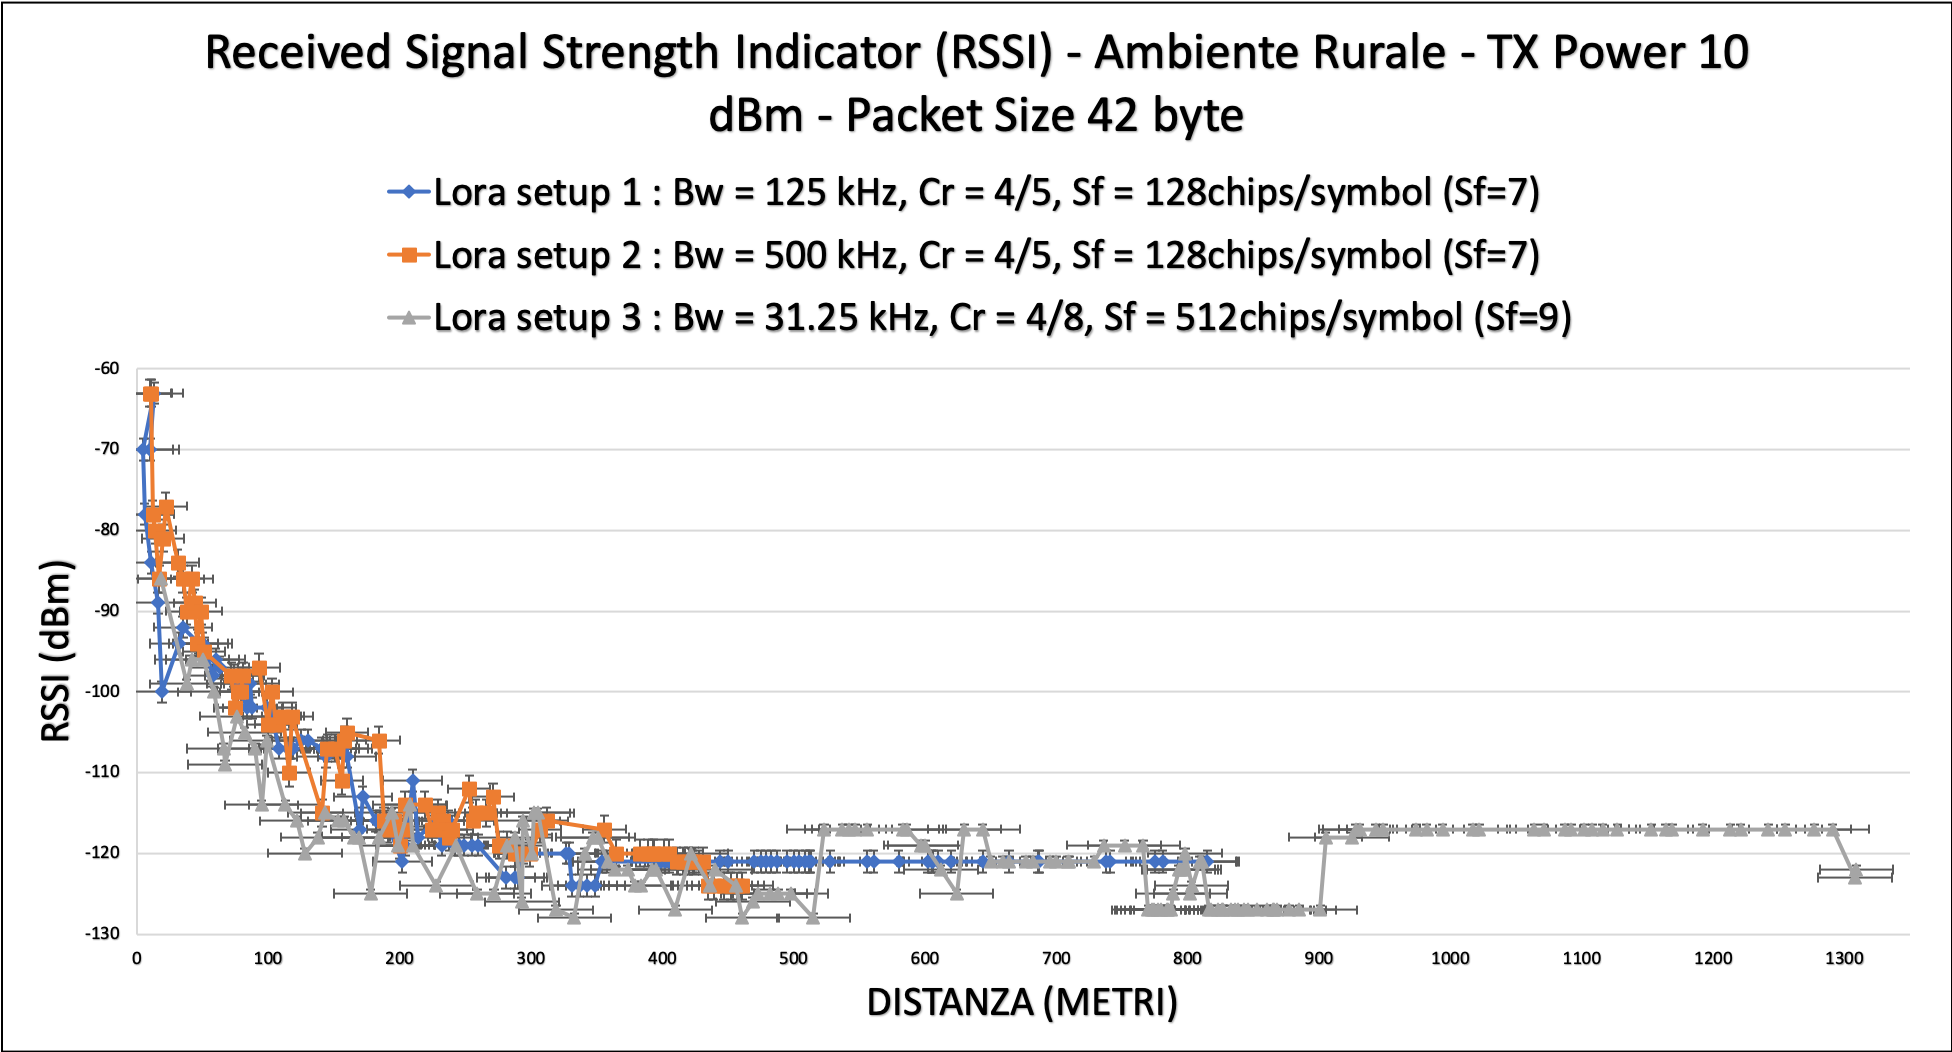
\includegraphics[width=\textwidth]{RSSI_confronto_AR-10dBm-42byte.png}
\caption[RSSI confronto Ambiente Rurale - 10 dBm - 42 byte]{RSSI confronto Ambiente Rurale - 10 dBm - 42 byte}\label{fig:prima}
\end{center}
\end{figure}

\begin{figure}[h]                      
\begin{center} 
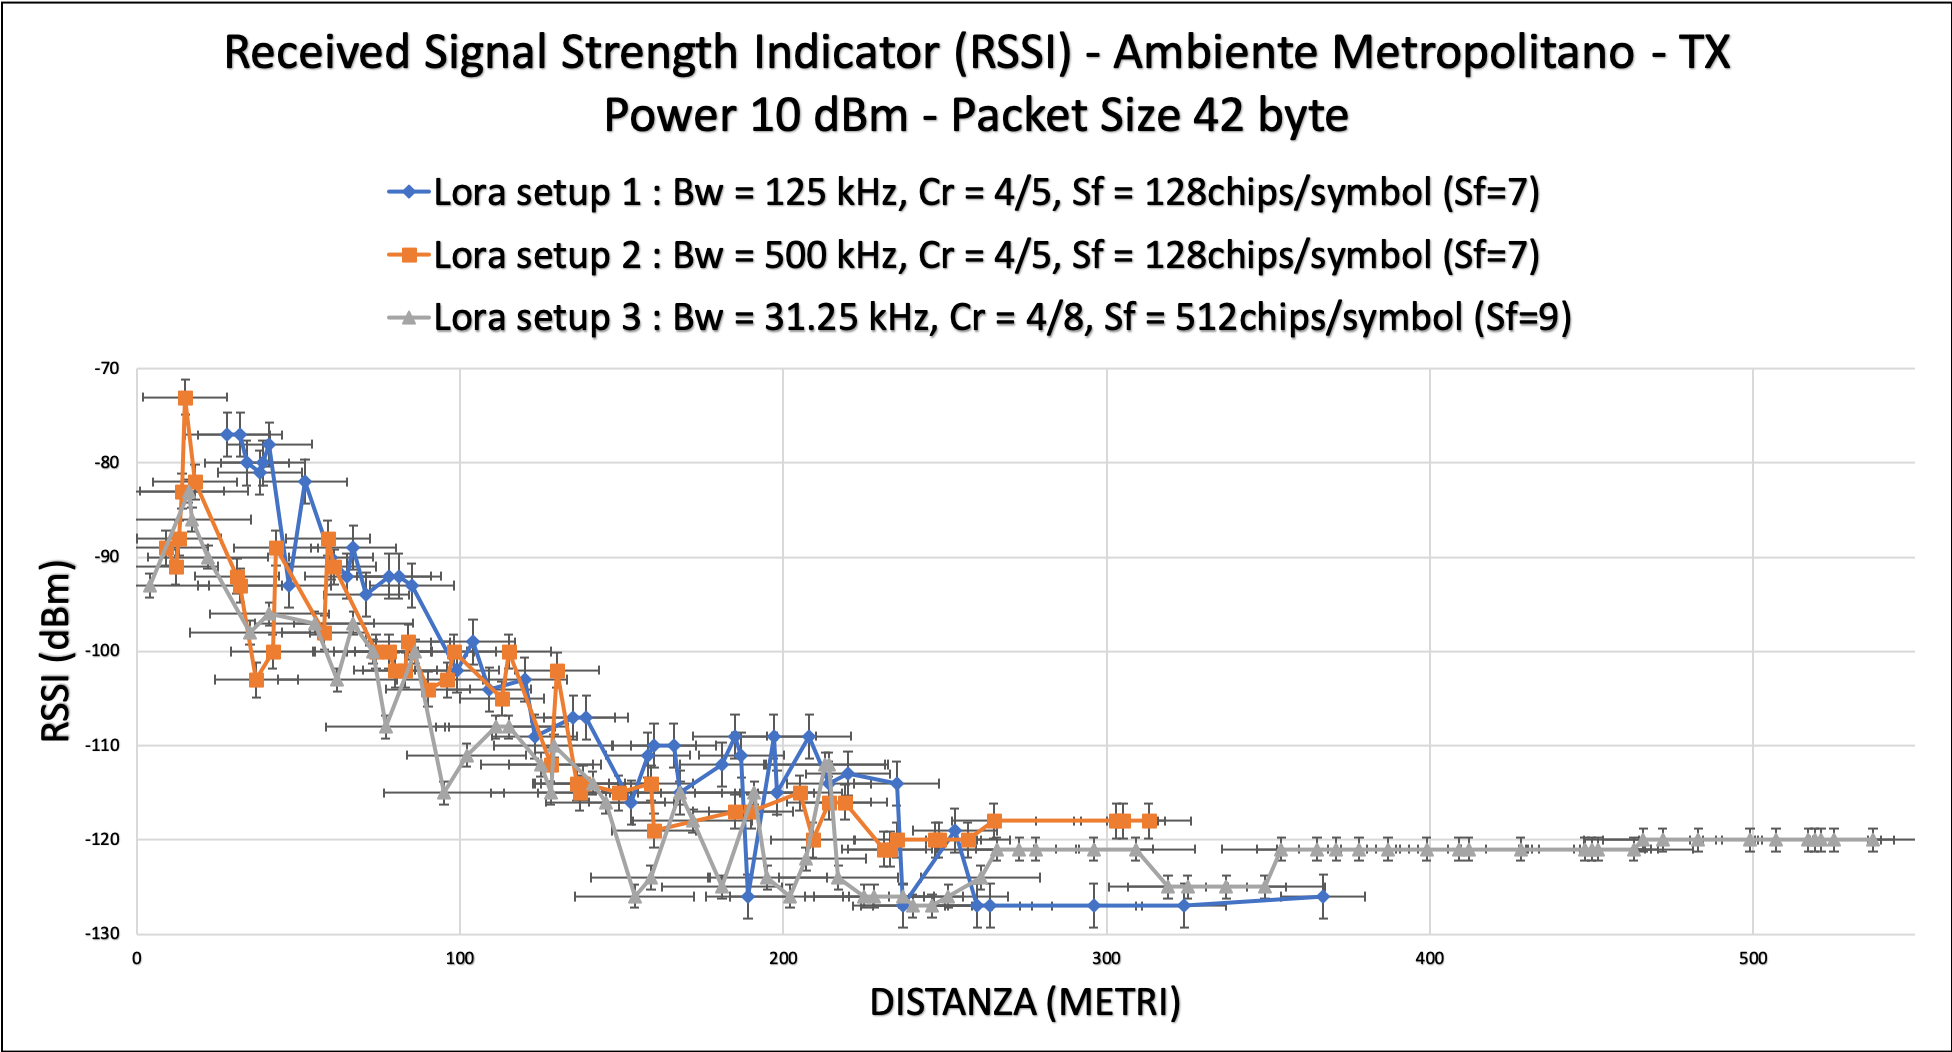
\includegraphics[width=\textwidth]{RSSI_confronto_AM-10dBm-42byte.png}
\caption[RSSI confronto Ambiente Metropolitano - 10 dBm - 42 byte]{RSSI confronto Ambiente Metropolitano - 10 dBm - 42 byte}\label{fig:prima}
\end{center}
\end{figure}

Risultati:
\begin{itemize}    
\item L'andamento del segnale \`e decrescente all'aumentare della distanza.
\item I tre setup LoRa non si discostano di molto tra loro nell'andamento e decresnono nello stesso modo.  
\item Il segnale trasmesso a 20 dBm \`e poco superiore alla media rispetto a 10 dBm. 
\item In AM ci sono oscillazioni di segnale pi\`u ampie rispetto ad AR a causa della forte presenza di ostacoli e rumore.
\item In AR si apprezzano maggiormente le differenze di potenza trasmessa. 
\end{itemize}

\subsection{Path Loss}
Il path loss \`e una misura che descrive l'attenuazione della potenza del segnale al variare della distanza. Il path loss viene calcolato in questo modo:
\begin{equation} TX POWER - RSSI \end{equation}
Questa misura \`e molto utile da tenere in considerazione quando si va ad effettuare un deploy in campo degli end node per stabilire le distanze ottimali a cui posizionare i dispositivi. Non essendoci differenze in merito ai tre setup LoRa, alla potenza trasmissiva e dimensione del pacchetto, si \`e scelto di mostrare un solo grafico campione che mostra l'andamento del path loss in AR e AM. Il setup utilizzato \`e LoRa 1. La figura 9.5 mostra la differenza tra path loss tra AR e AM. L'inclinazione della retta interpolante i punti fornisce un'idea di quanto rapidamente avviene l'attenuazione di segnale. In relazione ai risultati ottenuti dal test su RSSI i risultati ottenuti sono in linea con quelli attesi.

\begin{figure}[h]                      
\begin{center} 
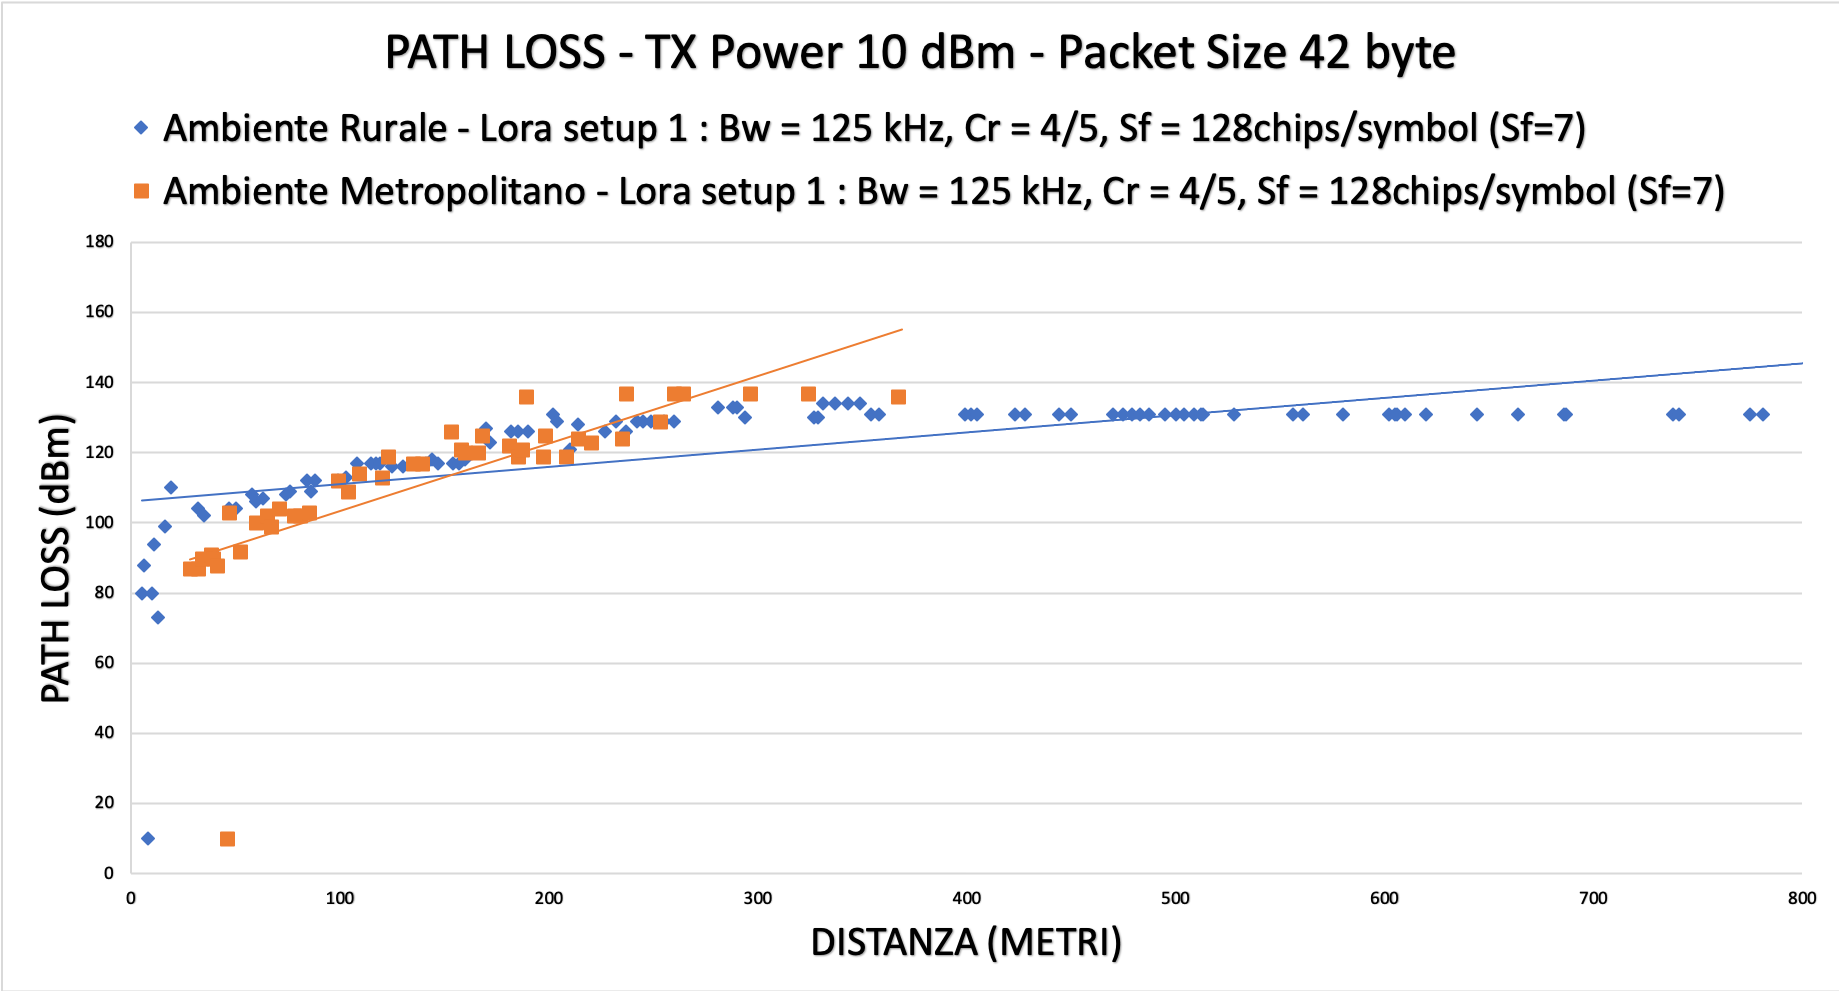
\includegraphics[width=\textwidth]{path_loss.png}
\caption[Path Loss confronto Ambiente Rurale e Ambiente Metropolitano - 10 dBm - 42 byte]{Path Loss confronto Ambiente Rurale e Ambiente Metropolitano - 10 dBm - 42 byte}\label{fig:prima}
\end{center}
\end{figure}

Risultati:
\begin{itemize}    
\item Senza considerare le distanze di copertura di segnale raggiunte, in AM l'inclinazione della retta che interpola i punti \`e maggiore rispetto all'inclinazione della retta in AR, in quanto l'interferenza e la presenza di ostacoli incidono molto sulla propagazione del segnale. 
\item In AM c'\`e una rapida perdita di segnale nei primi 200 metri.
\item In AR la perdita di segnale \`e meno brusca in quanto segue un andamento pi\`u uniforme che si stabilizza dopo i primi 200 metri.
\end{itemize}

\subsection{Delay}
Il delay rappresenta il tempo di trasmissione di un pacchetto da sorgente a destinazione espresso in millisecondi. Per il calcolo del delay sussiste un problema di temporizzazione in quanto i clock dell'end node e del gateway non sono sincronizzati, pertanto sarebbe impossibile calcolare la differenza di tempo tra l'invio e la ricezione del messaggio. Per questo motivo il delay viene calcolato dall'end node usando la funzione \textit{millis()}. Questa funzione restituisce il tempo trascorso dall'istante in cui \`e iniziato il programma, espresso in millisecondi. Questo valore viene incapsulato nel messaggio ed inviato al gateway il quale provvede a ritrasmettere all'end node il messaggio ricevuto. Alla ricezione del massaggio dal gateway l'end node estrae il valore precedentemente inserito e lo sottrae al nuovo valore restituito dalla funzione millis(). In questo modo si conosce per differenza di tempo il round trip time. Il RTT viene diviso per due in modo da conoscere il tempo effettivo di propagazione da sorgente a destinazione.  La figura 9.5 mostra il confronto tra i tre setup LoRa in termini di delay in ambiente rurale, mentre la figura 9.6 mostra il confronto del delay in ambiente metropolitano.

\begin{figure}[h]                      
\begin{center} 
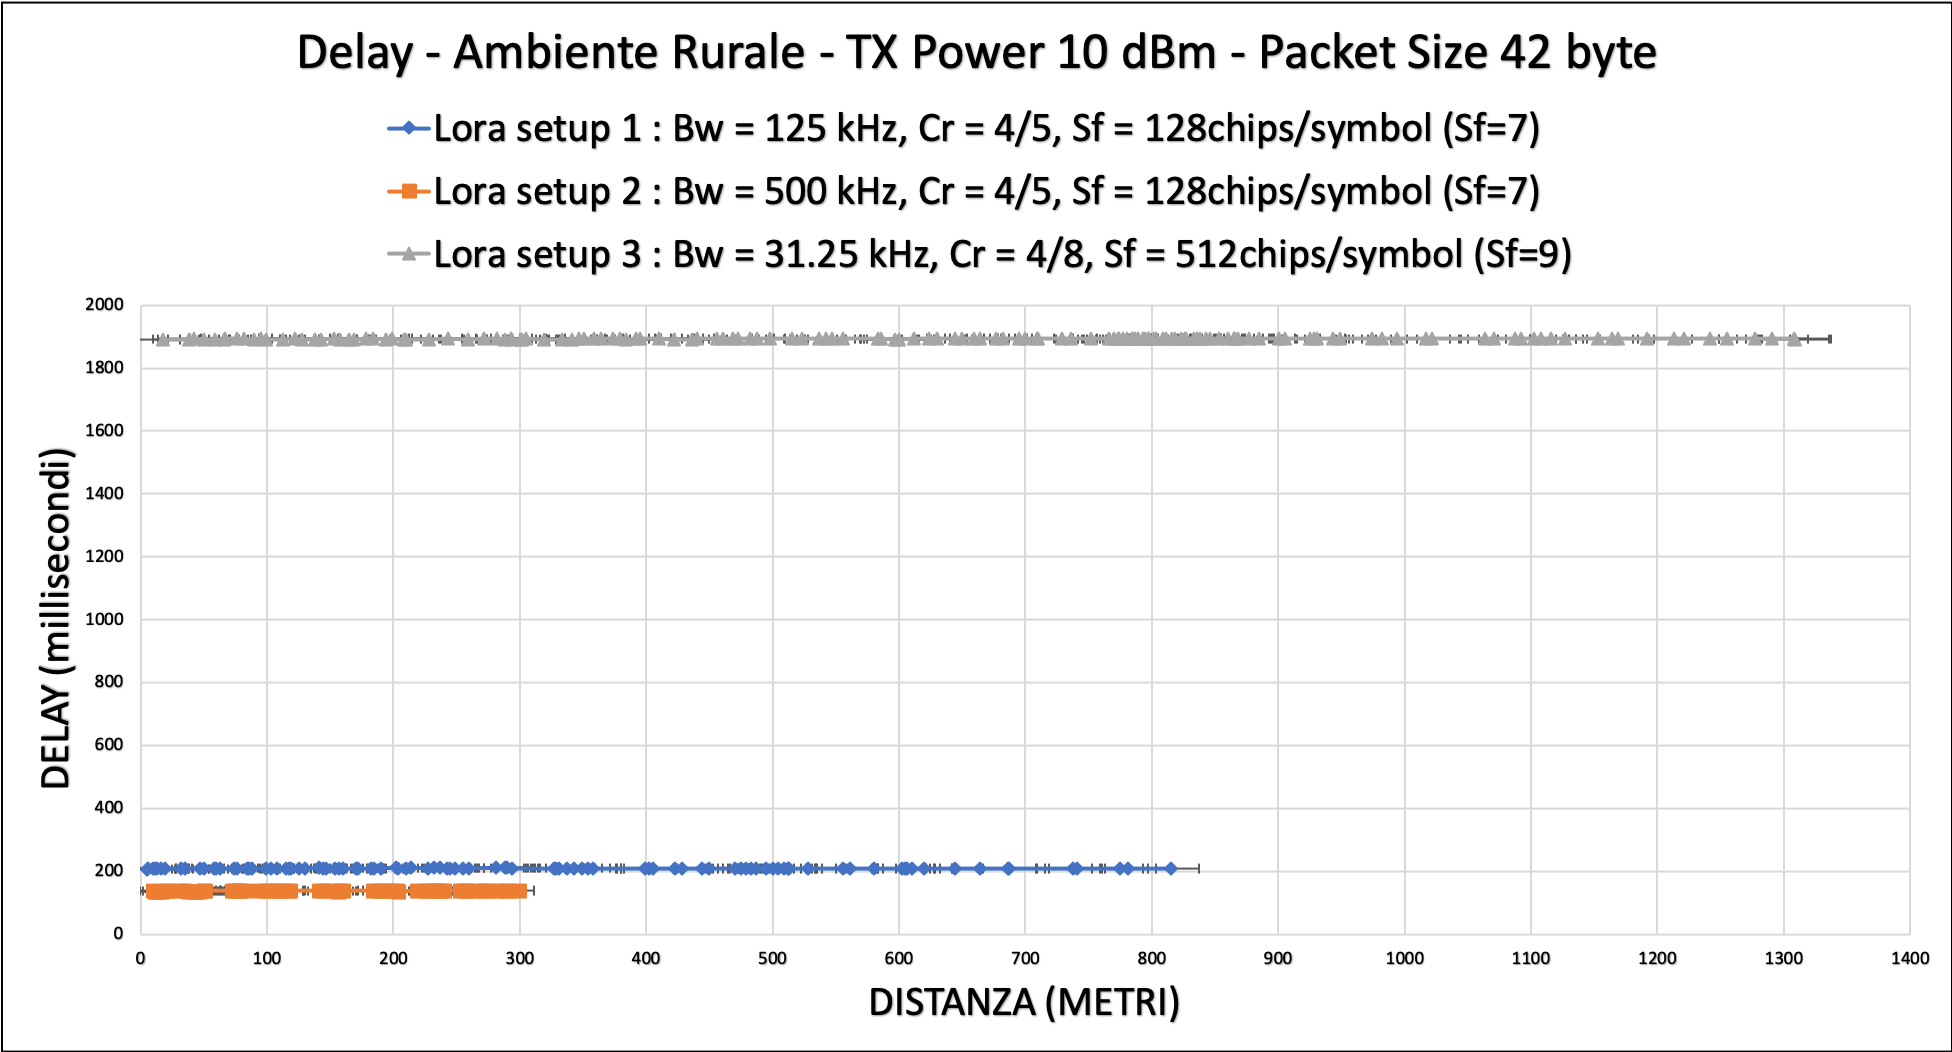
\includegraphics[width=\textwidth]{DELAY_confronto_AR_10dBm_42byte.png}
\caption[Delay confronto Ambiente Rurale - 10 dBm - 42 byte]{Delay confronto Ambiente Rurale - 10 dBm - 42 byte}\label{fig:prima}
\end{center}
\end{figure}

\begin{figure}[h]                      
\begin{center} 
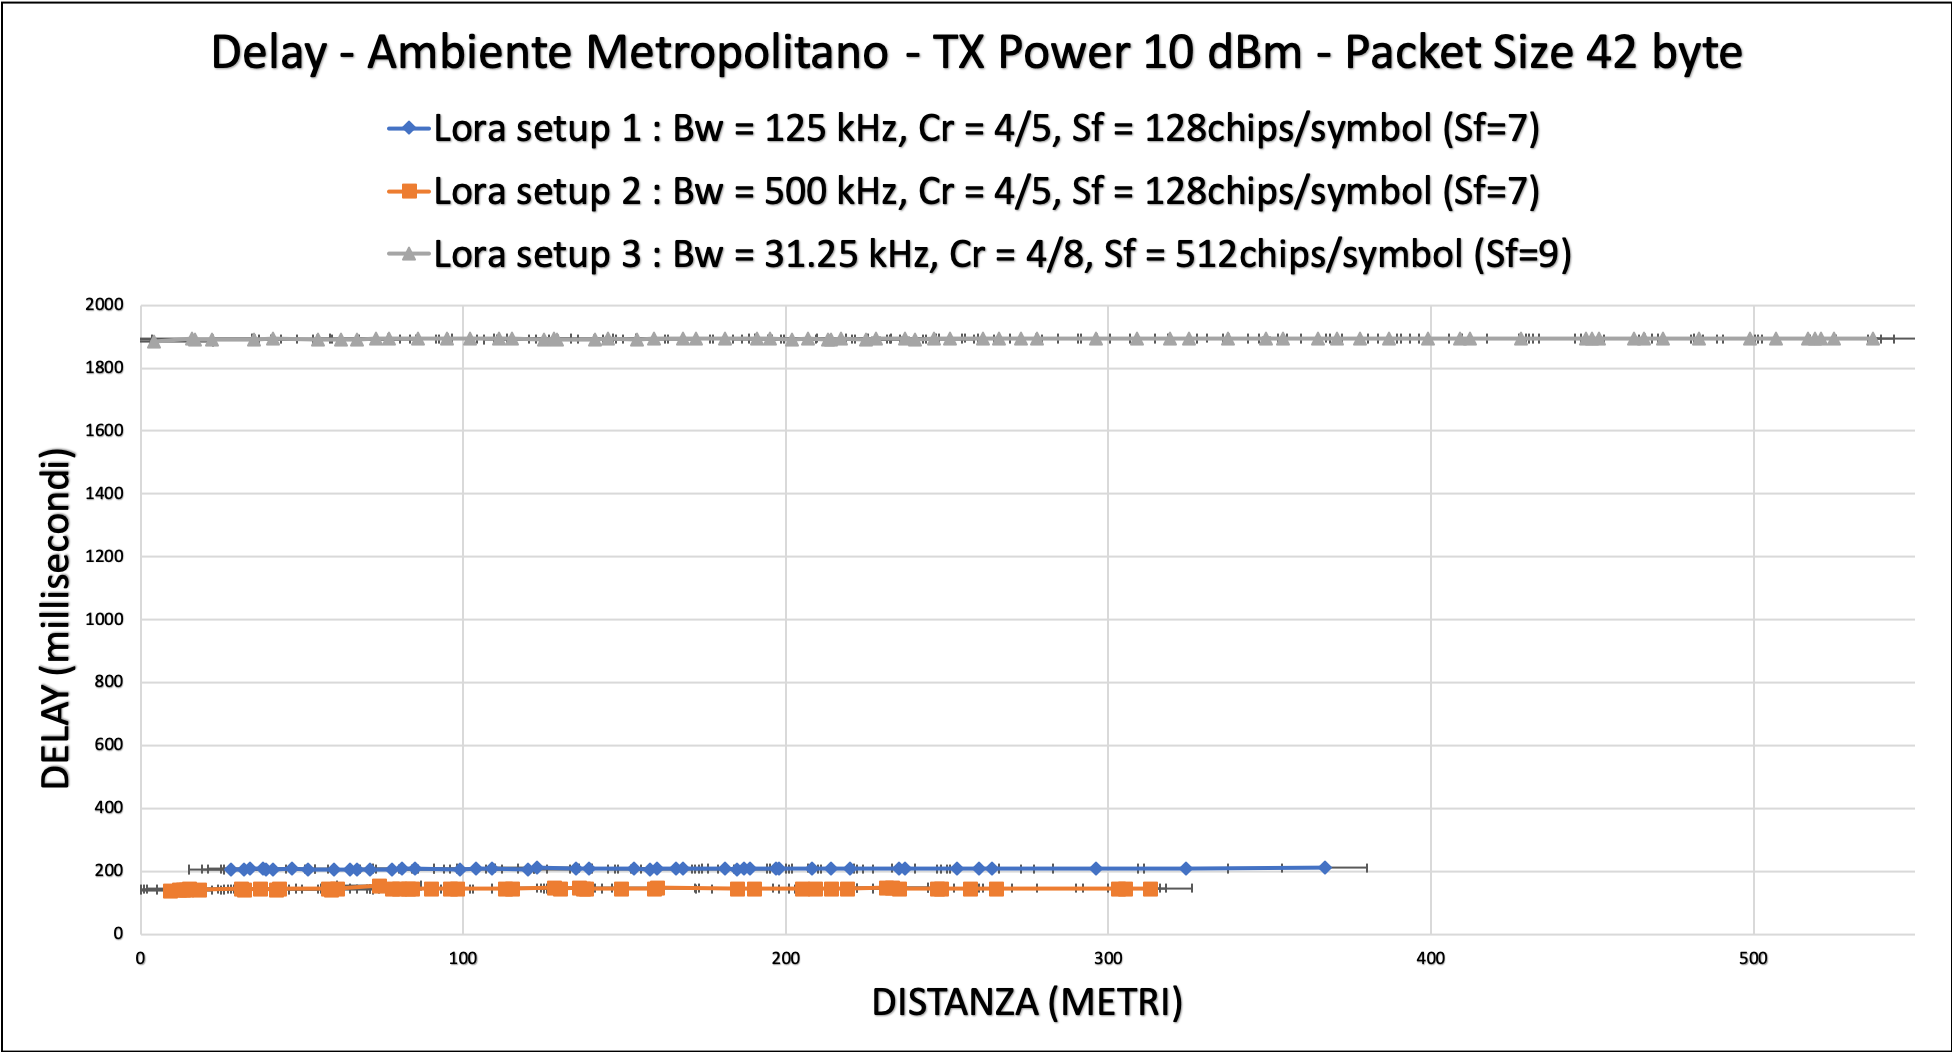
\includegraphics[width=\textwidth]{DELAY_confronto_AM_10dBm_42byte.png}
\caption[Delay confronto Ambiente Metropolitano - 10 dBm - 42 byte]{Delay confronto Ambiente Metropolitano - 10 dBm - 42 byte}\label{fig:prima}
\end{center}
\end{figure}

Risultati:
\begin{itemize}    
\item I tre setup LoRa differiscono di molto tra loro sui tempi di trasmissione, in quanto esiste una relazione diretta tra \textit{Spreading Factor} e delay. 
Il \textit{time on air} \`e pi\`u elevato in corrispondenza di un maggior valore di \textit{SF}, di conseguenza anche il delay \`e maggiore. 
\item In tutti gli esperimenti e per tutti i setup il delay segue un andamento lineare. Il motivo \`e dovuto dal fatto che le onde elettromagnetiche si propagano nello spazio alla velocit\`a della luce, pertanto la distanza percorsa non \`e significativa per avere impatti sul tempo di trasmissione.
\item Il setup LoRa 3 ha un valore di SF=9 pertanto il delay per questo setup \`e nettamente pi\`u elevato rispetto ai setup 1 e 2 che hanno entrambi valore di SF=7.
\item Il setup LoRa 2 ha il delay pi\`u basso rispetto a LoRa 1 in quanto a parit\`a di SF ha una ampiezza di banda del canale maggiore che si traduce in un sensibile miglioramento del tempo di trasmissione.
\item L'aumento di potenza del segnale non ha alcuna influenza sul delay.
\item I pacchetti con dimesione 84 byte hanno un delay maggiore rispetto a quelli a 42 byte.
\item Non ci sono differenze tra AR e AM.
\end{itemize}

\subsection{Capacit\`a di trasferimento}
La capacit\`a di trasferimento rappresenta in bitrate con cui vengono trasmessi i dati ed \`e stato calcolata dividendo la dimensione del pacchetto per il delay. Questa misura vine espressa in bps.
La dimensione del pacchetto \`e espressa in byte pertanto \`e stata convertita in bit, mentre il delay espresso in millisecondi \`e stao convertito in secondi.
Esiste una reazione inversa tra capacit\`a di trasferimento e delay, in quanto all'aumentare del delay diminuisce il bitrate. In questa sezione \`e stato scelto di non riportatare tutti i grafici relativi ai test, in quanto il bitrate ha un andamento costante e l'aumento di potenza trasmissiva o variazione di potenza non inficia il bitrate. La tabella 9.2 riepiloga i risultai ottenuti per le tre configurazioni LoRa con potenza trasmissiva pari a 10 dBm e dimensione del pacchetto pari a 42 byte. 

\begin{table}[h]                        
\begin{center}                          
\begin{tabular}{r|c|c}                  
$LoRa\ Setup$ & $Bitrate (bps)$ \\         
\hline\hline                                  
$1$ & $1600$\\     
\hline                               
$2$ & $2500$ \\
\hline        
$3$ & $180$\\ 
\hline \hline                         
\end{tabular}
\caption[Riepilogo capacit\`a di trasferimento]{Riepilogo capacit\`a di trasferimento}\label{tab:uno}
\end{center}
\end{table}

Risultati:
\begin{itemize}    
\item I tre setup LoRa presentano valori differenti tra loro.
\item Il bitrate migliore \`e relativo al setup 2 che si attesta attorno ai 2500 bps.
\item Il bitrate peggiore \`e relativo al setup 3 che si attesta attorno ai 180 bps.
\item Il setup LoRa 2 ha il delay pi\`u basso rispetto a LoRa 1 in quanto a parit\`a di SF ha una ampiezza di banda del canale maggiore che si traduce in un miglioramento del tempo di trasmissione.
\item L'aumento di potenza del segnale non ha alcuna influenza sul bitrate.
\item Non ci sono differenze tra AR e AM.
\end{itemize}

\subsection{Packet Delivery Ratio}
Il Packet Delivery Ratio (PDR) indica il rapporto tra numero di pacchetti trasmessi e numero di pacchetti ricevuti. Questa misura fornisce la stima di quanto sia affidabile il canale di comunicazione. La figura 9.8 mostra il confronto tra i tre setup LoRa in termini di PDR in AR, mentre la figura 9.9 mostra l'andamento del PDR in AM. 

\begin{figure}[h]                      
\begin{center} 
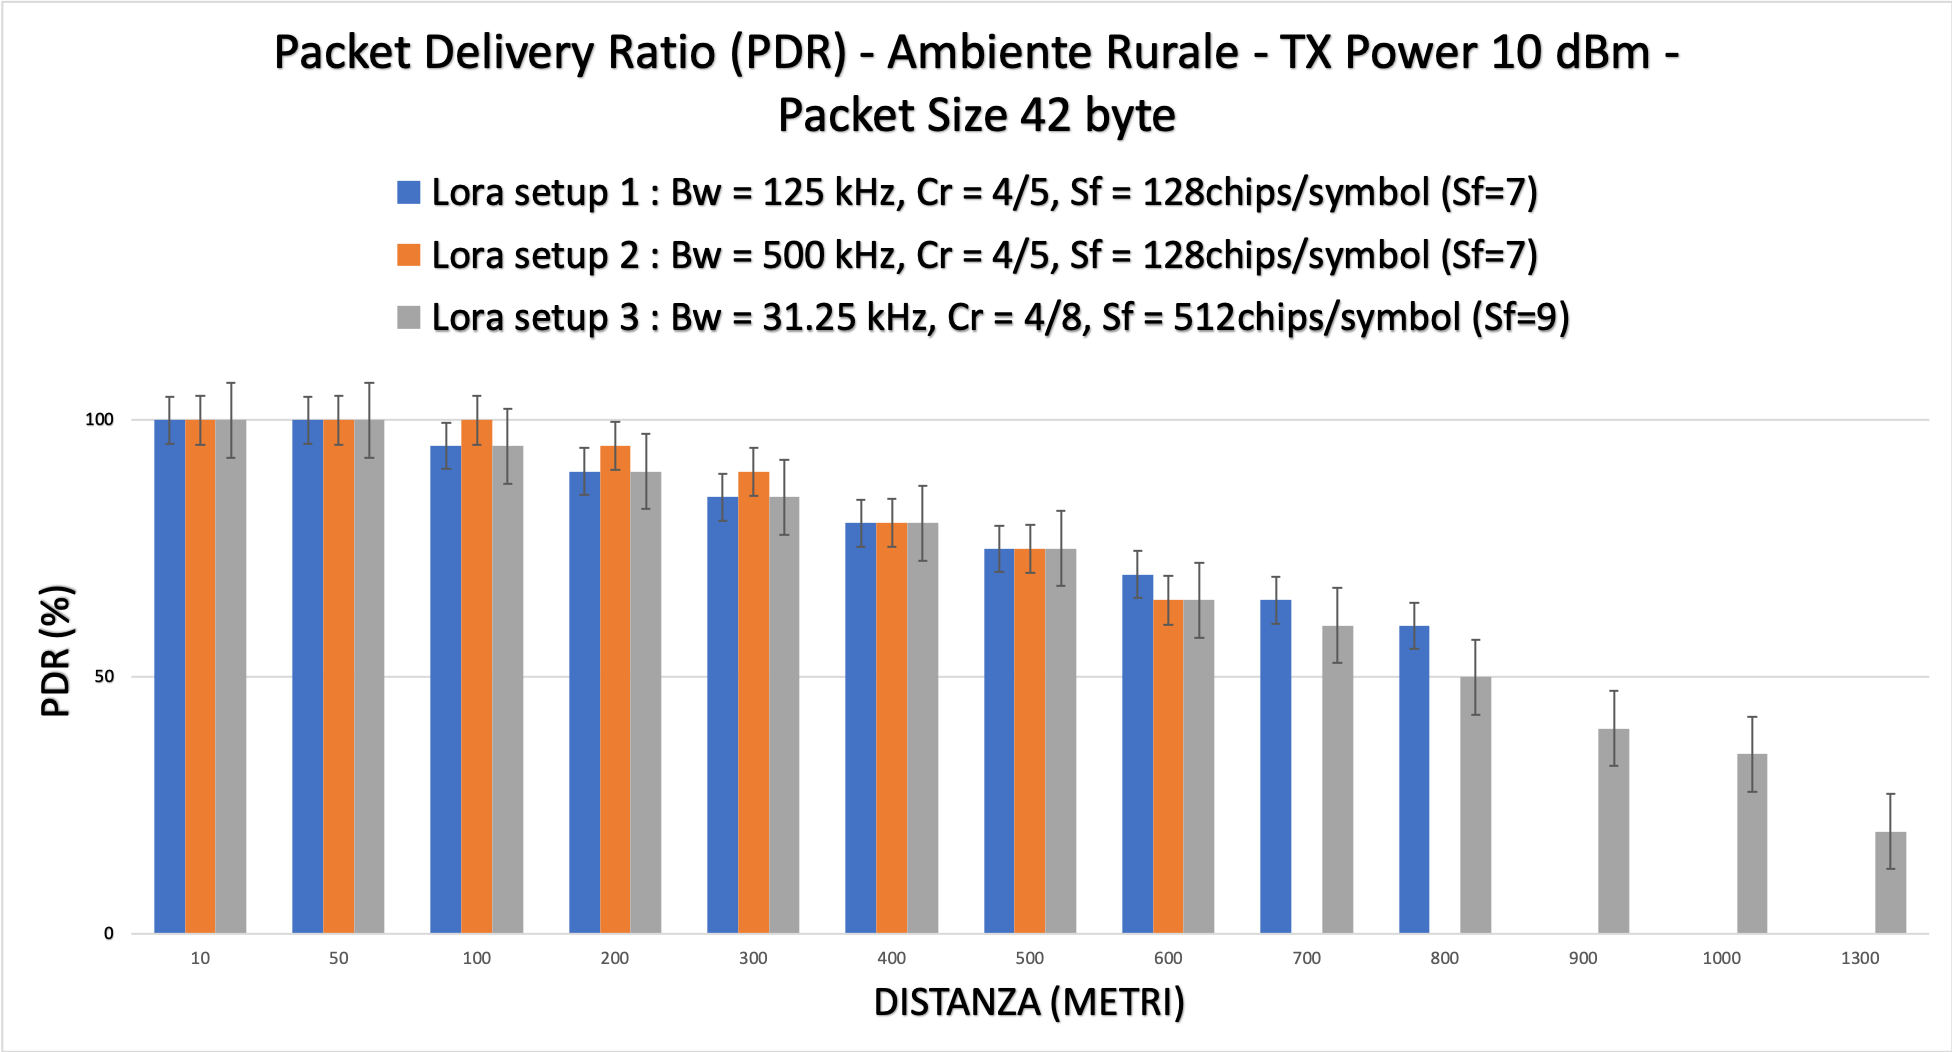
\includegraphics[width=\textwidth]{PDR_BAR_confronto_AR_10dBm-42byte.png}
\caption[Pdr confronto AR - 10 dBm - 42 byte]{Pdr confronto AR - 10 dBm - 42 byte}\label{fig:prima}
\end{center}
\end{figure}

\begin{figure}[h]                      
\begin{center} 
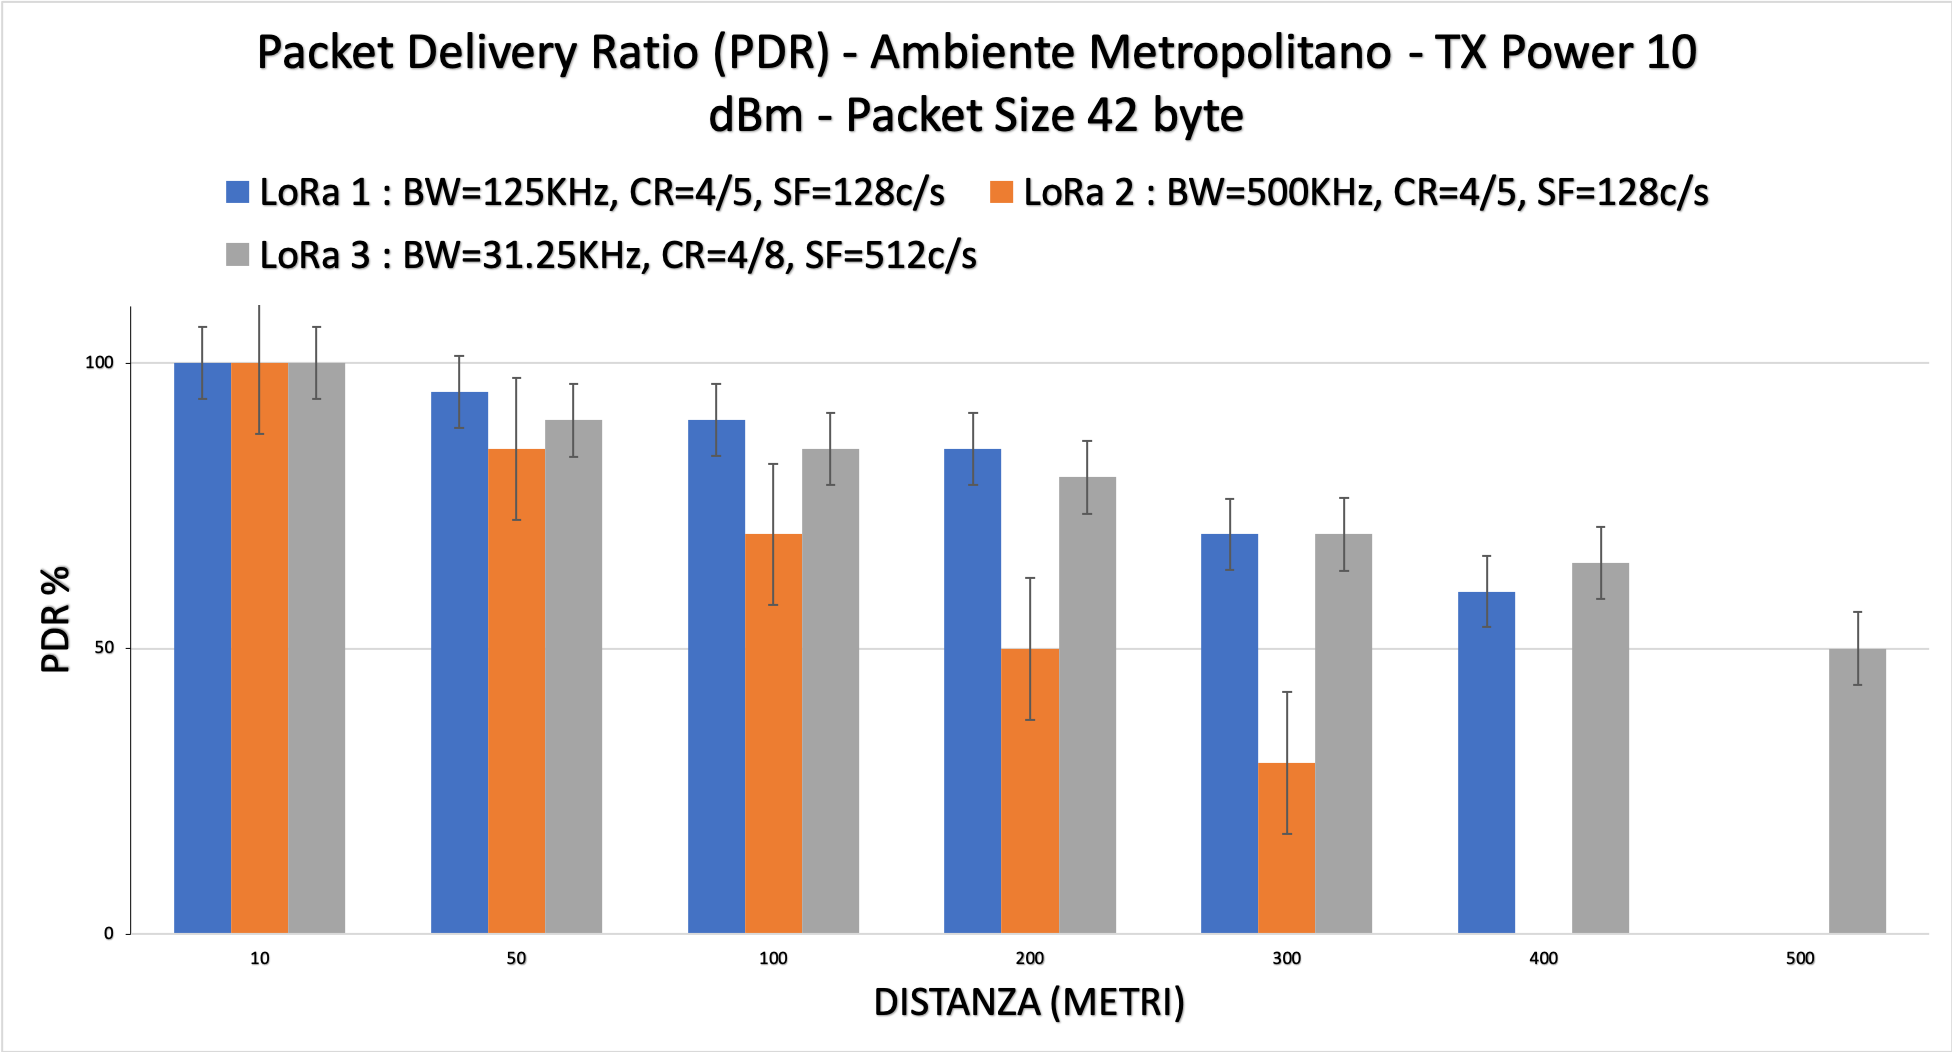
\includegraphics[width=\textwidth]{PDR_BAR_confronto_AM_10dBm-42byte.png}
\caption[Pdr confronto AM - 10 dBm - 42 byte]{Pdr confronto AM - 10 dBm - 42 byte}\label{fig:prima}
\end{center}
\end{figure}

Risultati:
\begin{itemize}    
\item Esistono sostanziali differenze in termini di PDR tra AR e AM. In AR il PDR \`e sempre mediamente pi\`u alto.
\item La dimensione del pacchetto ha un'incidenza maggiore sul PDR rispetto all'aumento di potenza trasmissiva, sopratutto considerato che in questa sperimentazione sono stati usati pacchetti di dimensioni elevate rispetto agli standard suggeriti dal produttore.  
\item L'aumento di potenza trasmissiva, a parit\`a di dimensione di pacchetto ha incidenza di miglioramento del 5\% circa in termini di pdr.  
\item I setup LoRa 1 e 2, a parit\`a di potenza trasmissiva e di dimensione di pacchetto risentono meno della variazione della dimensione del pacchetto in quanto la bandwidth consente il trasporto di pacchetti a 84 byte.
\item In AM il setup Lora 2 risente maggiormente dell'interferenza a causa della bandwidth pi\`u ampia rispetto agli altri setup. Se i canali sono stretti c'\`e meno interferenza di rumore esterno. Al contrario, in AR, lo stesso setup in virt\`u della maggiore bandwidth risente nel trasporto di pacchetti a dimensione di 84 byte
\item Il setup LoRa 3 risente maggiormente nel trasporto di pacchetti a 84 byte perch\`e la bandwidth non \`e sufficiente al trasporto dei dati. Questo si traduce in una minore distanza raggiunta in quanto il PDR a a distanze superiori a 800 metri diventa quasi pari a zero. 
\item L'aumento di potenza trasmissiva fa aumentare la distanza di copertura di circa cento metri.
\end{itemize}



\chapter{Sviluppi futuri e conclusioni}
Gli ambiti applicativi che afferiscono sotto la dicitura Internet Of Things sono innumerevoli ed eterogenei, pertanto non esiste una soluzione tecnologica generica che possa coprire qualsiasi scenario. 
Le tecnologie LPWAN nascono dall'esigenza di disporre di trasmissioni a lungo raggio, con basso data rate e poco consumo energetico. Come ampiamente discusso nel capitolo tre esiste ad oggi una pletora di tecnologie LPWAN. Su tutte, LoRa, sta riscuotendo grande attenzione e successo grazie alle performance che riesce a garantire.
In attesa dell'arrivo del 5G, ad oggi esistono soluzioni concorrenti a LoRa.
Nell'ambito delle Smart Cities, dove le reti cellulari offrono una copertura capillare del segnale, si predilige un approccio in cui si sfruttano le infrastrutture esistenti senza doverne implementare di nuove. Diverso il discorso in ambito rurale, dove la scarsa copertura di segnale cellulare offre potenziali aree di intervento. In questo contesto LoRa garantisce degli ottimi risultati soprattutto in ambito di monitoraggio ambientale e agricoltura di precisione. Inoltre, considerato il fatto che LoRa opera in uno spettro di frequenza ISM che non \`e sottoposto a vincoli di licenza, il livello di interferenza da parte di altre trasmissioni \`e molto pi\`u basso in ambito rurale, pertanto si riescono a raggiungere ottime prestazioni.    
In fase di analisi preliminare di un'applicazione IoT quando si fanno valutazioni su quale tecnologia possa essere pi\`u idonea alla progettazione bisogna considerare i seguenti fattori:
 \begin{itemize}                       
\item Distinguere se l'applicazione \`e delay tolerant o real time.
\item Identificare l'area di copertura del segnale radio di cui si ha bisogno.
\item Stimare la dimensione dei dati trasmettere.
\item Valutare se le trasmissioni avvengono in luoghi chiusi o all'aperto.
\item Fare una stima di quanto pu\`o essere critico la perdita di un pacchetto al verificarsi di un evento.
\item Calcolare il consumo energetico qualora si adoperassero dispositivi alimentati da batteria.
\item Fare una stima dei costi di deploy relativa al numero di dispositivi minimi sufficienti per il sensing e l'automation.
\end{itemize}

In questa tesi si \`e visto come sia possibile realizzare un'infrastruttura LoRaWAN, in grado di gestire i dati ambientali dalla raccolta all'analisi. 
Grazie agli esperimenti condotti, si \`e in grado di avere una stima di quali sono le performance relative alla trasmissione LoRa. Sulla base delle metriche raccolte \`e possibile fare tuning della configurazione del trasmettitore radio in modo da poter disporre del miglior setup.  

Dai test effettuati \`e emerso che la trasmissione LoRa garantisce prestazioni migliori in ambito rurale. Per la sperimentazione \`e stato scelta una localit\`a rurale totalmente priva di ostacoli ed i test sono stati condotti fuori dalla stagione vegetativa quindi in assenza di colture. Questo tipo di scenario \`e poco realistico in quanto anche in ambito rurale esistono abitazioni (anche se sporadiche) e ci potrebbero essere ostacoli come gli alberi. 
In alcuni casi l'abito rurale potrebbe avere forti impatti del degrado della trasmissione. Ad esempio alcuni test sono stato fatti in parchi urbani caratterizzati dalla presenza di qualche albero ma privi di abitazioni. I risultati ottenuti non si discostano molto dai test fatti in ambiente metropolitano con la presenza di palazzi. Questo potrebbe essere causato non solo dalla presenza degli alberi che fanno da ostacoli ma anche dalle interferenze radio dovute a trasmissioni che operano nello stesso spettro.  
Il contesto che pi\`u si avvicina all'ambiente rurale \`e la spiaggia priva di stabilimenti balneari e persone. Alcuni ricercatori hanno dimostrato \cite{K28} che per applicazioni di monitoraggio delle imbarcazioni entro un raggio di qualche chilometro dal porto \`e possibile ottenere ottimi risultati in termini di PDR. In questa ricerca, ad esempio, \`e stata sviluppata un'applicazione per la raccolta delle metriche relative alla navigazione. Le imbarcazioni a vela che si allenavano in vista delle olimpiadi sono state equipaggiate con dispositivi LoRa in grado di raccogliere diverse metriche. Come dimostrato nella ricerca il segnale LoRa si propaga molto bene in mare aperto, pertanto potrebbe essere utile per lo sviluppo di applicazioni per piccoli pescherecci che pescano entro un raggio di qualche chilometro dalla riva.  

La sperimentazione si \`e concentrata sull'analisi delle metriche relative alla trasmissione tra un end device ed il gateway. Quando si parla di WSN (Wireless Sensor Network) bisogna considerare scenari possibili in cui potenzialmente potrebbero essere messi in produzione anche centinaia o migliaia di dispositivi che comunicano contemporaneamente. 
In questo scenario andrebbe fatta una sperimentazione sulla misurazione della scalabilit\`a della rete, in quanto, uno dei punti deboli della trasmissione LoRa \`e il protocollo Aloha che regolamenta le politiche di accesso al mezzo da parte del trasmettitore radio. 
Questo protocollo, a differenza di CSMA/CA, \`e pi\`u semplice da implementare ma non fornisce garanzie sul recapito dei messaggi in caso di collisione. Per questo motivo sarebbe utile fare una sperimentazione su quanto una rete LoRAWAN sia effettivamente affidabile e scalabile in presenza di centinaia di dispositivi che trasmettono contemporaneamente.   

Gli esperimenti condotti sono stati fatti secondo due modalit\`a. La prima consiste nel raccogliere le metriche stando fermi in uno specifico punto (a distanze prefissate) per un certo tempo al fine di poter analizzare il packet delivery ratio. La seconda modalit\`a consiste nell'effettuare una ``passeggiata'' allontanandosi gradualmente dal nodo gateway, per poter valutare come variano le metriche in funzione della distanza. In relazione alla prima modalit\`a di test sarebbe interessare analizzare quali sono le performance prendendo un arco di tempo molto ampio come ad esempio un anno, in modo tale da verificare se ci sono differenze nella trasmissione con l'alternarsi delle stagioni. Bisognerebbe studiare l'impatto di agenti esterni come l'umidit\`a presente nell'aria. L'infrastruttura implementata in questa tesi pu\`o essere adoperata per condurre questo esperimento in quanto l'end device da me realizzato \`e dotato di sensore DHT11 che misura la temperatura e l'umidit\`a, mentre la piattaforma di data analytics pu\`o memorizzare ed organizzare grandi moli di dati. 

In questa tesi non \`e stato affrontato il tema del consumo energetico da parte di LoRa. Il motivo principale \`e che non si dispone di strumenti specifici che misurino l'impatto della trasmissione LoRa sulle batterie. In ottica di sviluppi futuri sarebbe utile raccogliere le metriche relative al consumo energetico in modo da poter ottenere il miglior valore per il duty cycle.   

Per un'analisi pi\`u precisa bisognerebbe adottare degli accorgimenti che potrebbero migliorare i risultati ottenuti in questa sperimentazione. In entrambi gli ambienti di test l'antenna del gateway non era posizionata in maniera adeguata. In ambiente metropolitano il gateway \`e stato posizionato sul balcone al secondo piano di un palazzo pertanto sarebbe stato opportuno quantomeno posizionarlo sul terrazzo. In ambiente rurale il gateway \`e stato appoggiato sul tettuccio dell'auto. In questo modo il segnale si propaga ground to ground, ma la carrozzeria dell'auto potrebbe fare interferenza. Sarebbe stato pi\`u opportuno posizionare l'antenna del gateway su un palo. 

L'architettura LoRaWAN implementata in questa tesi \`e semplificata rispetto alle specifiche, in quanto priva del ruolo di network server. Il motivo deriva dal fatto che avendo usato un solo nodo come end device non vi era l'esigenza di usare il network server che tra le principali funzionalit\`a assolve il compito di eliminare eventuali pacchetti duplicati e di gestire ADR (Adaptive Data Rate) una funzionalit\`a attraverso la quale il network server fornisce indicazioni all'end device su come configurare i parametri della trasmissione LoRa in base alla qualit\`a del segnale. In un'ottica di implementazione di una rete LoRa composta da pi\`u dispositivi sarebbe utile analizzare come cambiano le performance relative alla trasmissione in presenza della funzionalit\`a di ADR.         

Sebbene i sensori (soprattutto in ambito di monitoraggio ambientale) producono piccole quantit\`a di dati la frequenza con la quale vengono inviati pu\`o produrre volumi consistenti.  
Per questo motivo si preferisce adottare database basati su paradigma NoSQL che garantiscono una maggiore scalabilit\`a in relazione alla gestione dei Big Data. I sistemi di data analytics lavorano dell'ottica di valutare quali sono gli andamenti su serie temporali ampie dei dati anzich\`e su una singola rilevazione. Tuttavia per prevedere gli andamenti futuri servono strumenti di Intelligenza Artificiale basati su meccanismi di machine learning. Nell'ambito del monitoraggio ambientale, ad esempio, seguendo la variazione di temperatura e umidit\`a pregressi \`e possibile fare una previsione sulle condizioni future. 

In estrema sintesi analizzando i dati della sperimentazione \`e possibile affermare che i risultati  ottenuti (con le dovute limitazioni) sono in linea con quanto dichiarato da Semtech. 
Riepilogando sinteticamente \`e emerso quanto segue:
\begin{itemize}                       
\item In ambiente rurale \`e possibile ottenere ottime performance non solo perch\`e ci sono meno ostacoli e quindi meno fenomeni di rifrazione e deviazione del segnale, ma perch\`e c'\`e anche meno interferenza dovuta alla trasmissione da parte di altre tecnologie radio che trasmettono sulla stessa frequenza. Si ricorda che LoRa utilizza la banda ISM non sottoposta a licenza in cui operano molte altre tecnologie radio.
\item Il setup 1 (medium range) rappresenta il miglior compromesso tra distanza e tempo di trasmissione. Il delay \`e leggermente inferiore al setup 2 tuttavia si riesce ad ottenere una distanza maggiore ed anche un livello di PDR mediamente pi\`u elevato.
La dimensione della bandwidth rappresenta un giusto compromesso tra delay e capacit\`a di trasporto dei dati. Questo tipo di setup pu\`o essere impiegato come configurazione di default per iniziare a sperimentare una qualsiasi applicazione.
\item Il setup 2 (fast + short range) offre ottimi tempi di nella trasmissione dei dati, ma ha lo svantaggio di avere un raggio di copertura molto basso. In ambito metropolitano risente molto delle interferenze a causa della bandwidth pi\`u ampia rispetto agli altri due setup, e quindi pi\`u suscettibile ad interferenza. Questo tipo di configurazione pu\`o essere impiegata in applicazioni in cui si necessita di bassa latenza e non si ha il vincolo di operare su una lunga distanza. Un esempio potrebbero essere sistemi di allarme o di rilevazione di condizioni di pericolo. 
\item Il setup 3 (long range) \`e in grado di raggiungere le distanze maggiori ma con delle latenze molto alte. La bandwidth \`e di soli 31,5 KHz pertanto insufficiente al trasporto di pacchetti di grandi dimensioni. Bisogna considerare che alle lunghe distanze bisogna inviare pacchetti di dimensioni inferiori a 40 byte. 
Questa configurazione pu\`o essere impiegata in ambito di monitoraggio ambientale in cui non c'\`e alcun requisito sui tempi di trasmissione ma si ha l'esigenza di avere ampia copertura sul territorio.
\item La dimensione dei pacchetti utilizzata nella sperimentazione \`e troppo elevata. Semtech consiglia di usare pacchetti di dimensione tra i 10 e 40 byte. Dai test \`e emerso che usando pacchetti di dimensione pari a 84 byte le prestazioni peggiorano soprattutto per il setup 3. Considerato che ai fini del consumo energetico \`e pi\`u dispendiosa la trasmissione dei dati rispetto alla computazione, bisogna ricordare che esiste un trade off tra dimensione dei dati da trasmettere e capacit\`a computazionali dell'end device. In linea di massima si preferisce avere un end device con scarse capacit\`a di calcolo, pertanto i dati grezzi non vengono processati dal dispositivo ma dai sistemi di backend. 
Ovviamnete spedire pi\`u dati grezzi implica avere maggiori impatti sulla trasmissione. I risultati ottenuti dalla sperimentazione dicono che l'invio di pacchetti di dimensioni superiori ai 40 byte provocano un degrado di permorfance in termini di distanza raggiunta e PDR, perci\`o considerato che i costi di produzione delle cpu degli end device si sono ridotti, converrebbe impiegare dei dispositivi in grado di effettuare calcoli sui dati grezzi al fine di trasmettere pacchetti con dimensioni ridotte. 
In questo modo, in caso di collisione, la ritrasmissione \`e meno costosa.
Dal punto di vista della potenza del segnale \`e emerso che il valore pari a 10 dBm (quanto consigliato dal produttore) rappresenta un livello ottimale, in quanto raddoppiando la potenza trasmissiva si ottiene un miglioramento medio del 5\% in termini di PDR e al pi\`u si raggiunge una distanza superiore di circa cento metri. Tuttavia, anche se non \`e stata fatta una sperimentazione specifica a riguardo in questa tesi, si avrebbe un forte impatto sul consumo energetico e quindi sulla durata delle batterie.   
\end{itemize}
L'infrastruttura realizzata, basata su rete LoRaWAN per la raccolta e trasmissione di dati associata alla piattaforma di data analytics con search engine NoSQL, si \`e dimostrata un ottimo supporto per lo sviluppo di applicazioni IoT in ambito di monitoraggio ambientale.
\appendix
\chapter{Grafici sperimentazione}
\begin{figure}[h]                      
\begin{center} 
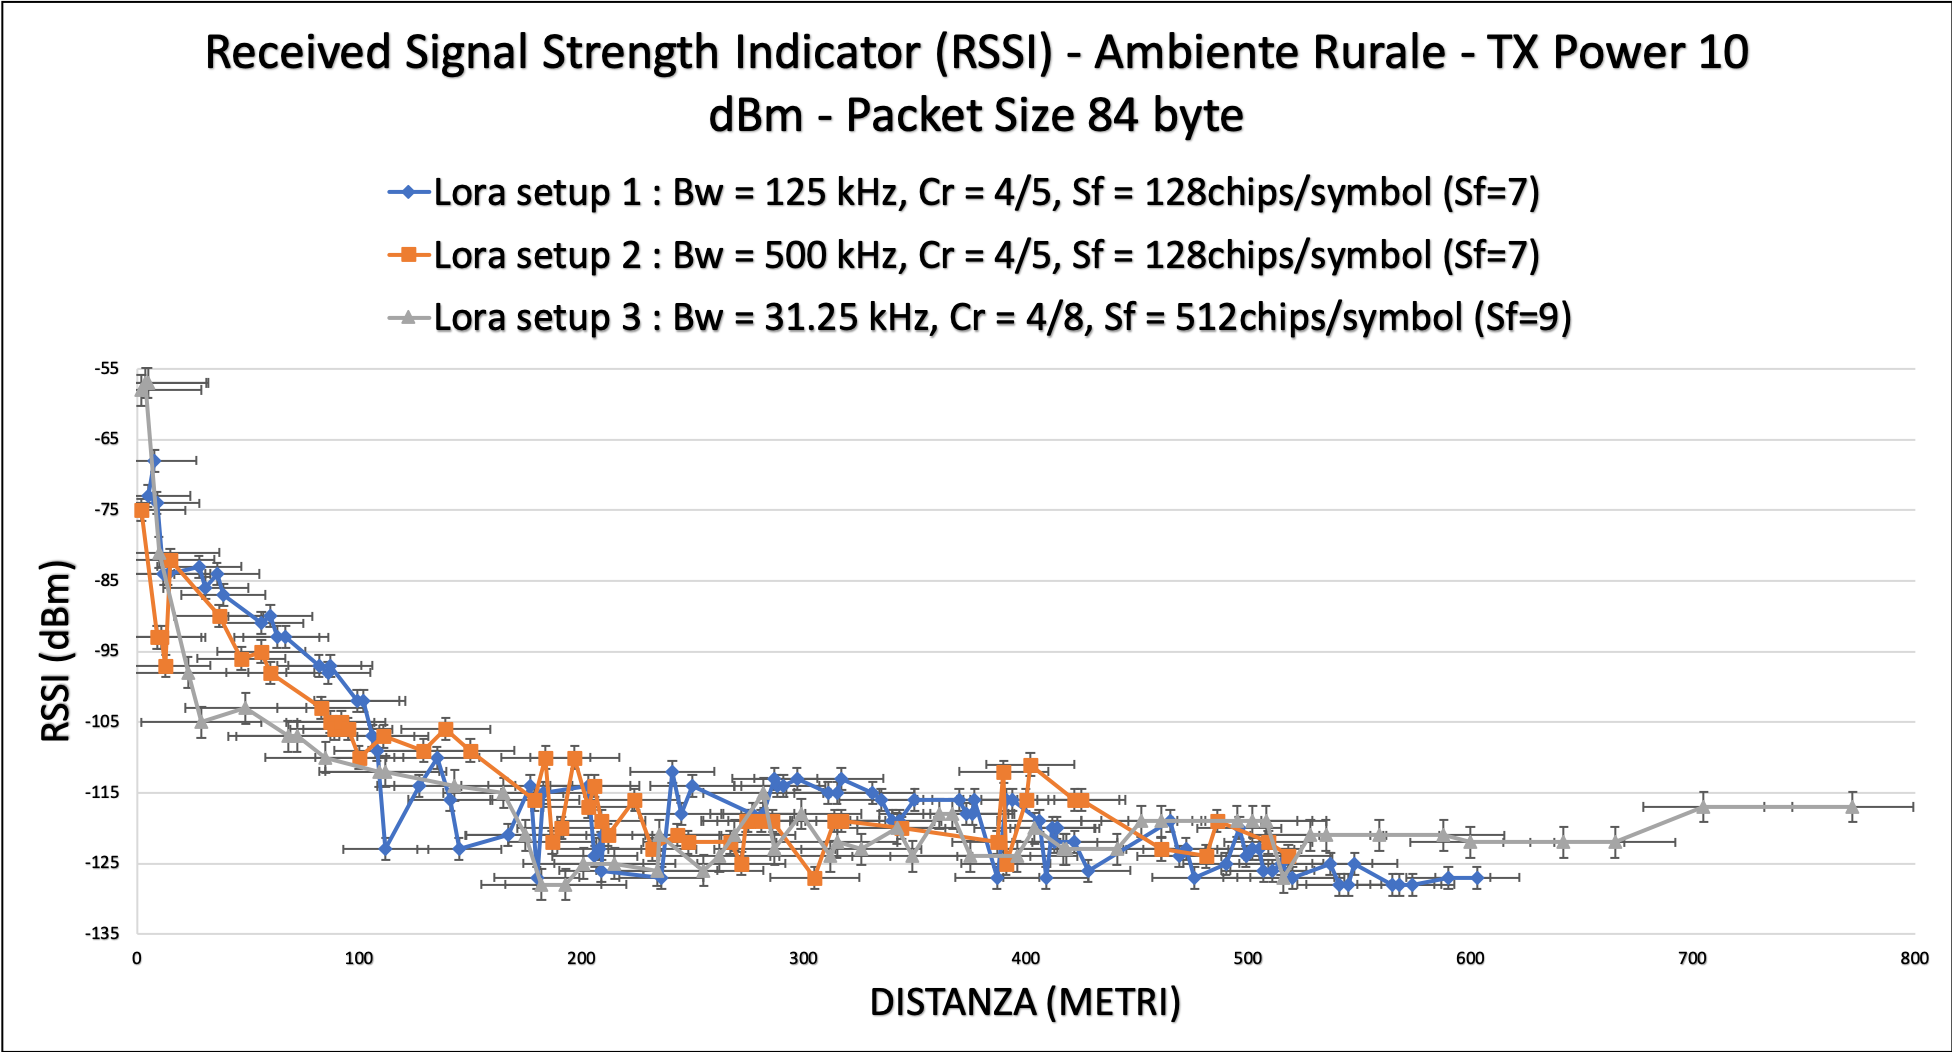
\includegraphics[width=\textwidth]{RSSI_confronto_AR-10dBm-84byte.png}
\caption[RSSI confronto Ambiente Rurale - 10 dBm - 84 byte]{RSSI confronto Ambiente Rurale - 10 dBm - 84 byte}\label{fig:prima}
\end{center}
\end{figure}

\begin{figure}[h]                      
\begin{center} 
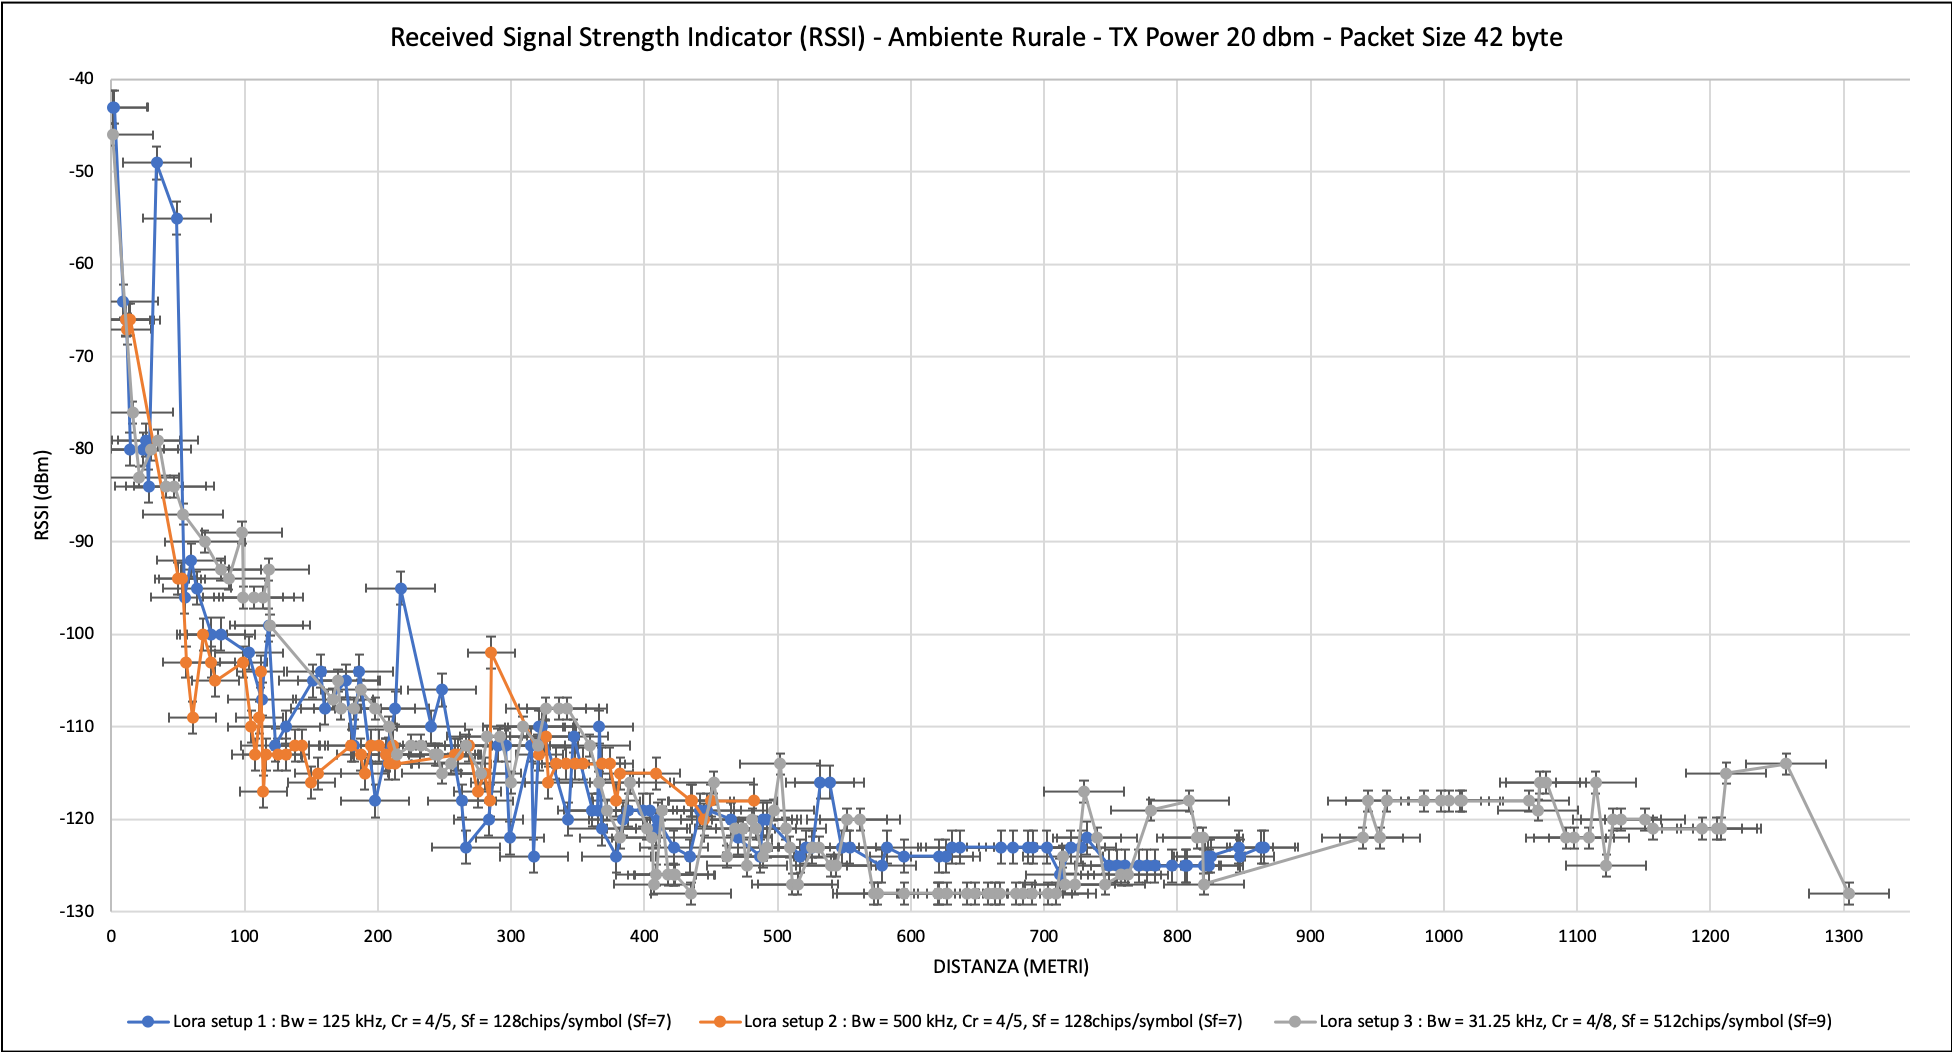
\includegraphics[width=\textwidth]{RSSI_confronto_AR_20dBm-42byte.png}
\caption[RSSI confronto Ambiente Rurale - 20 dBm - 42 byte]{RSSI confronto Ambiente Rurale - 20 dBm - 42 byte}\label{fig:prima}
\end{center}
\end{figure}

\begin{figure}[h!]                      
\begin{center} 
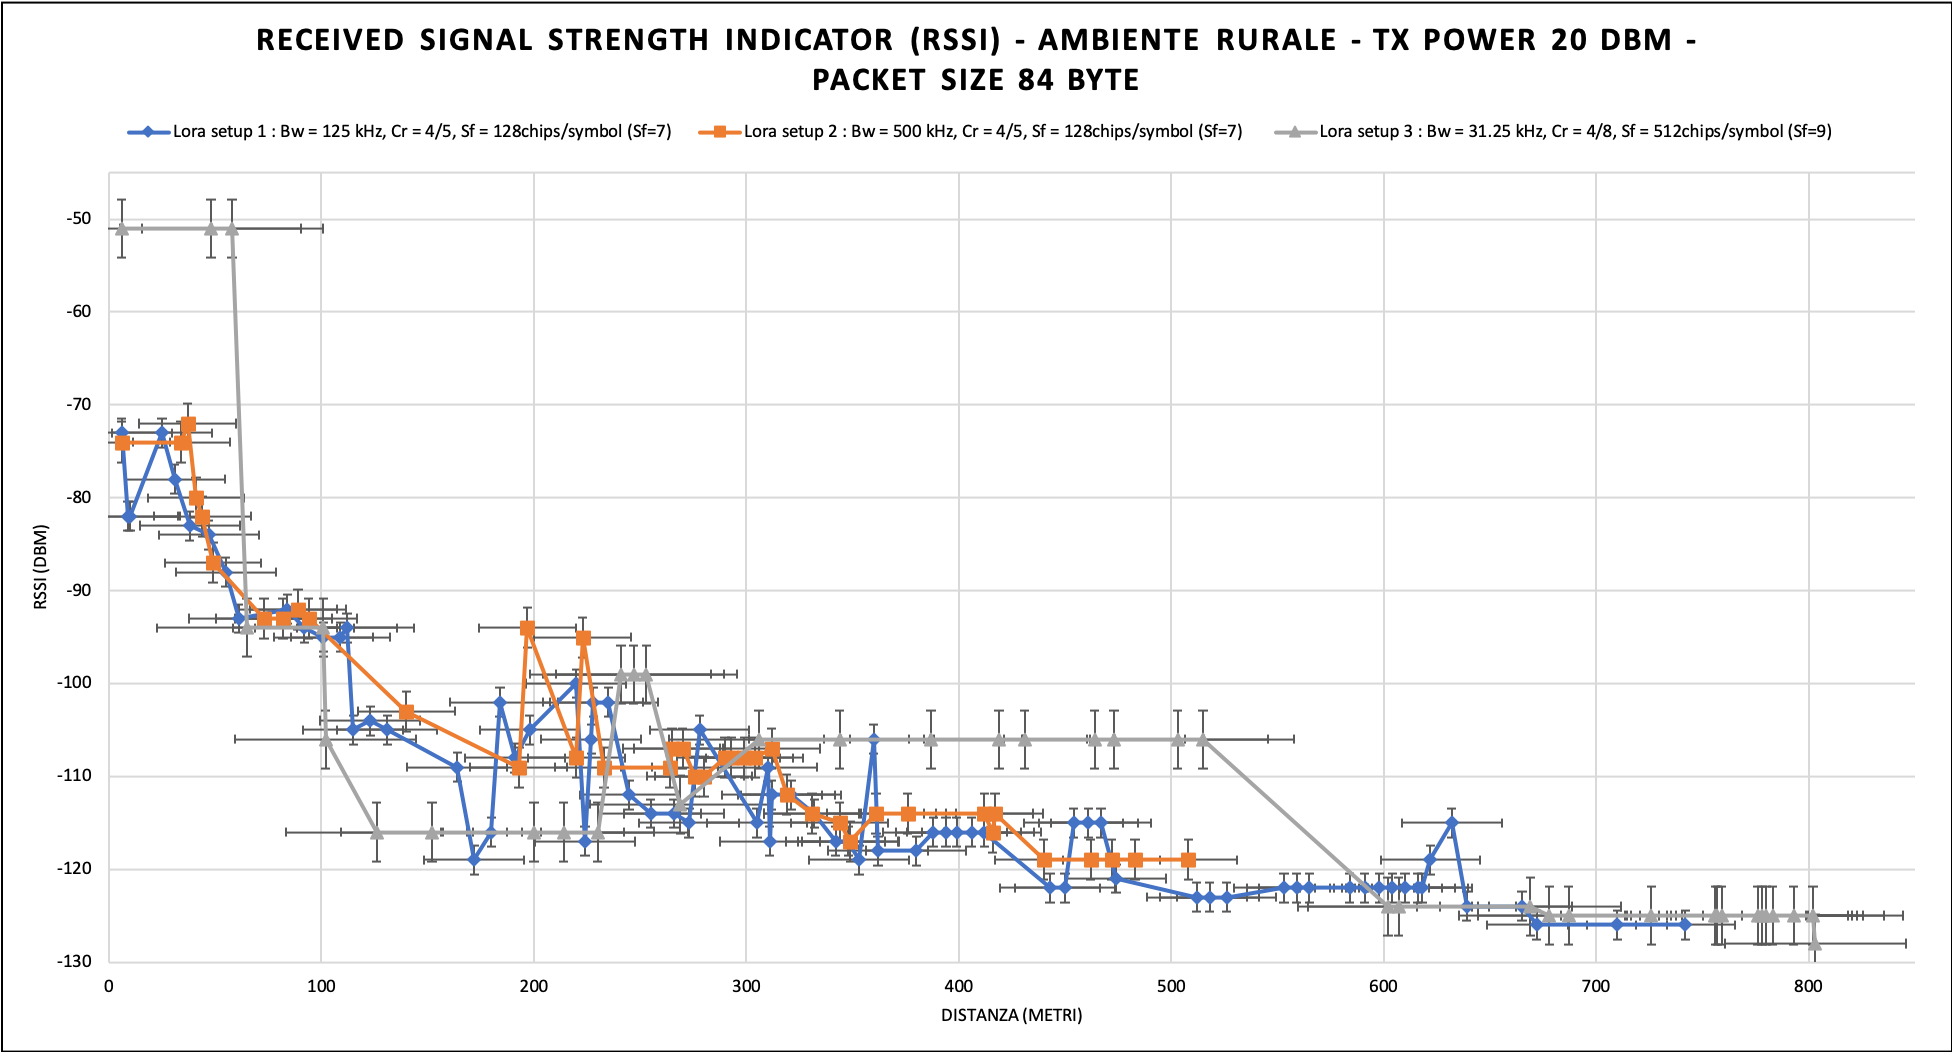
\includegraphics[width=\textwidth]{RSSI_confronto_AR-20dBm-84byte.png}
\caption[RSSI confronto Ambiente Rurale - 20 dBm - 84 byte]{RSSI confronto Ambiente Rurale - 20 dBm - 84 byte}\label{fig:prima}
\end{center}
\end{figure}

\begin{figure}[h!]                      
\begin{center} 
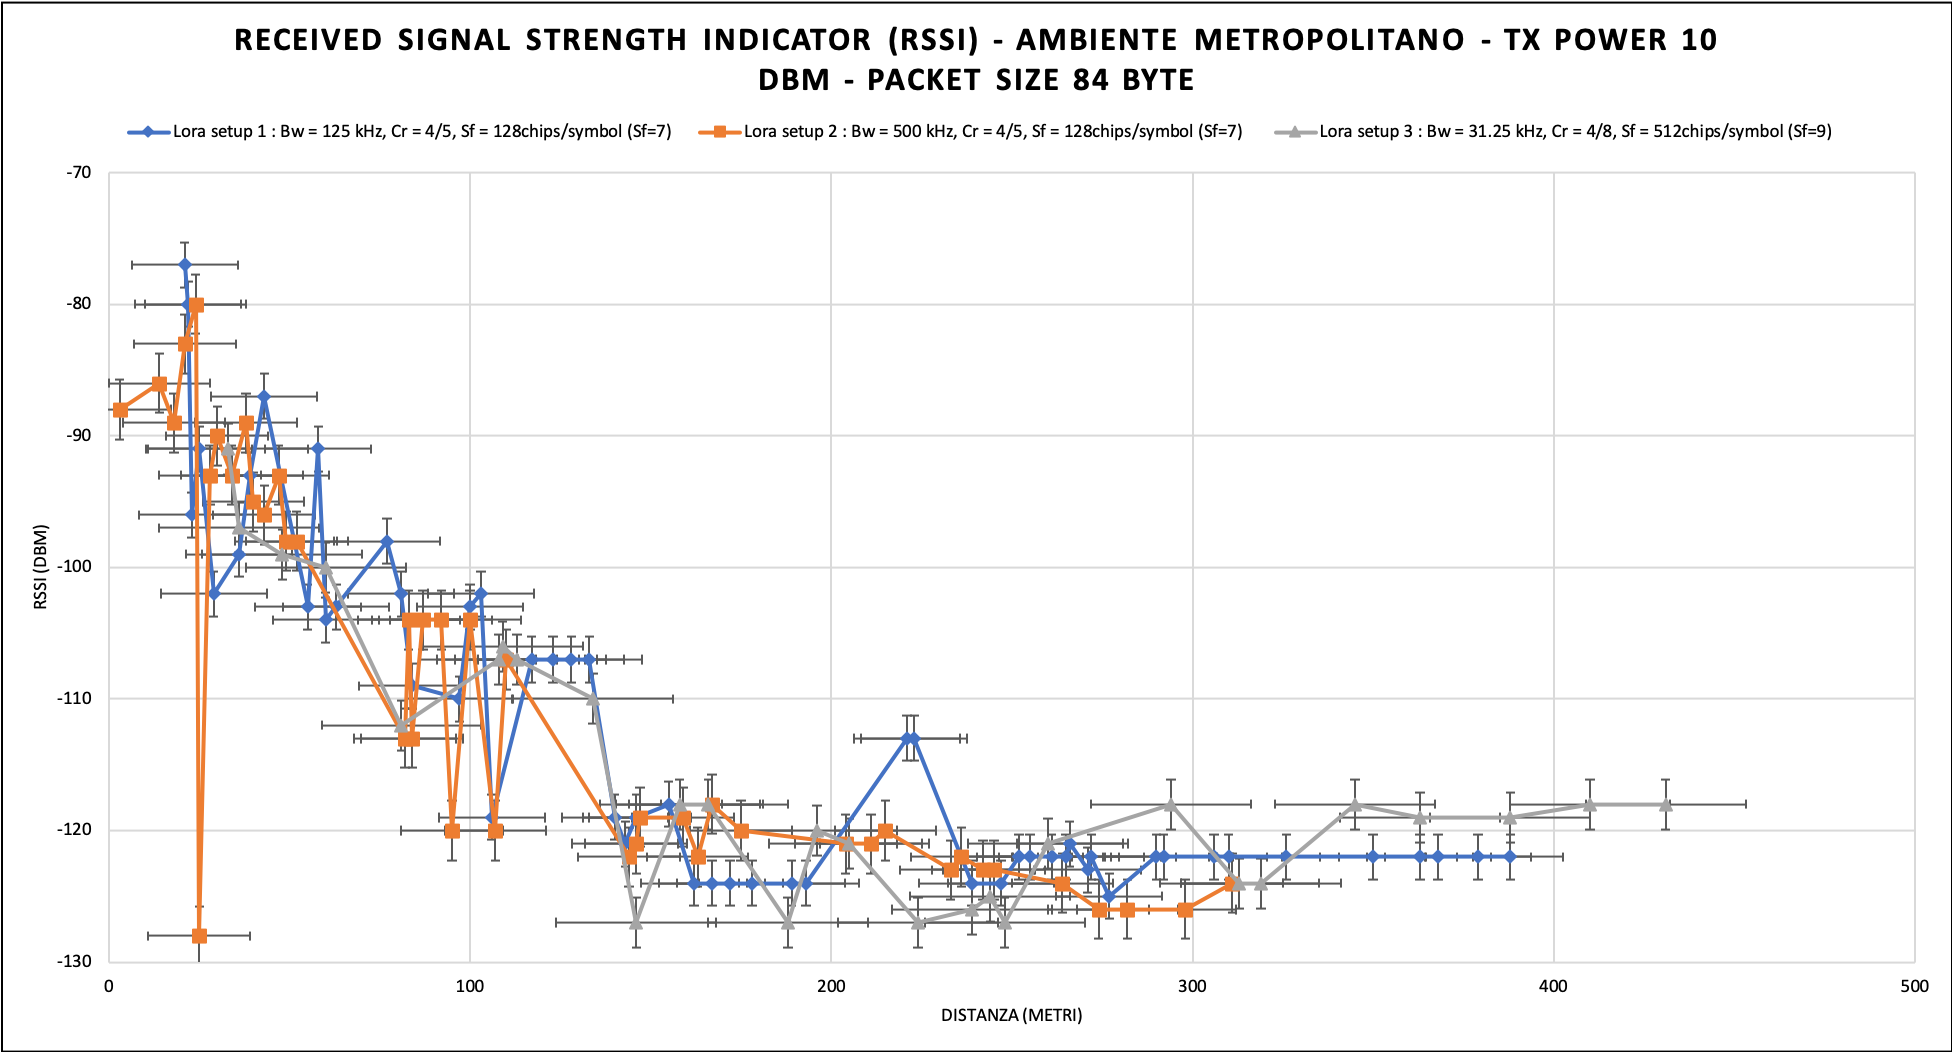
\includegraphics[width=\textwidth]{RSSI_confronto_AM-10dBm-84byte.png}
\caption[RSSI confronto Ambiente Metropolitano - 10 dBm - 84 byte]{RSSI confronto Ambiente Metropolitano - 10 dBm - 84 byte}\label{fig:prima}
\end{center}
\end{figure}

\begin{figure}[h]                      
\begin{center} 
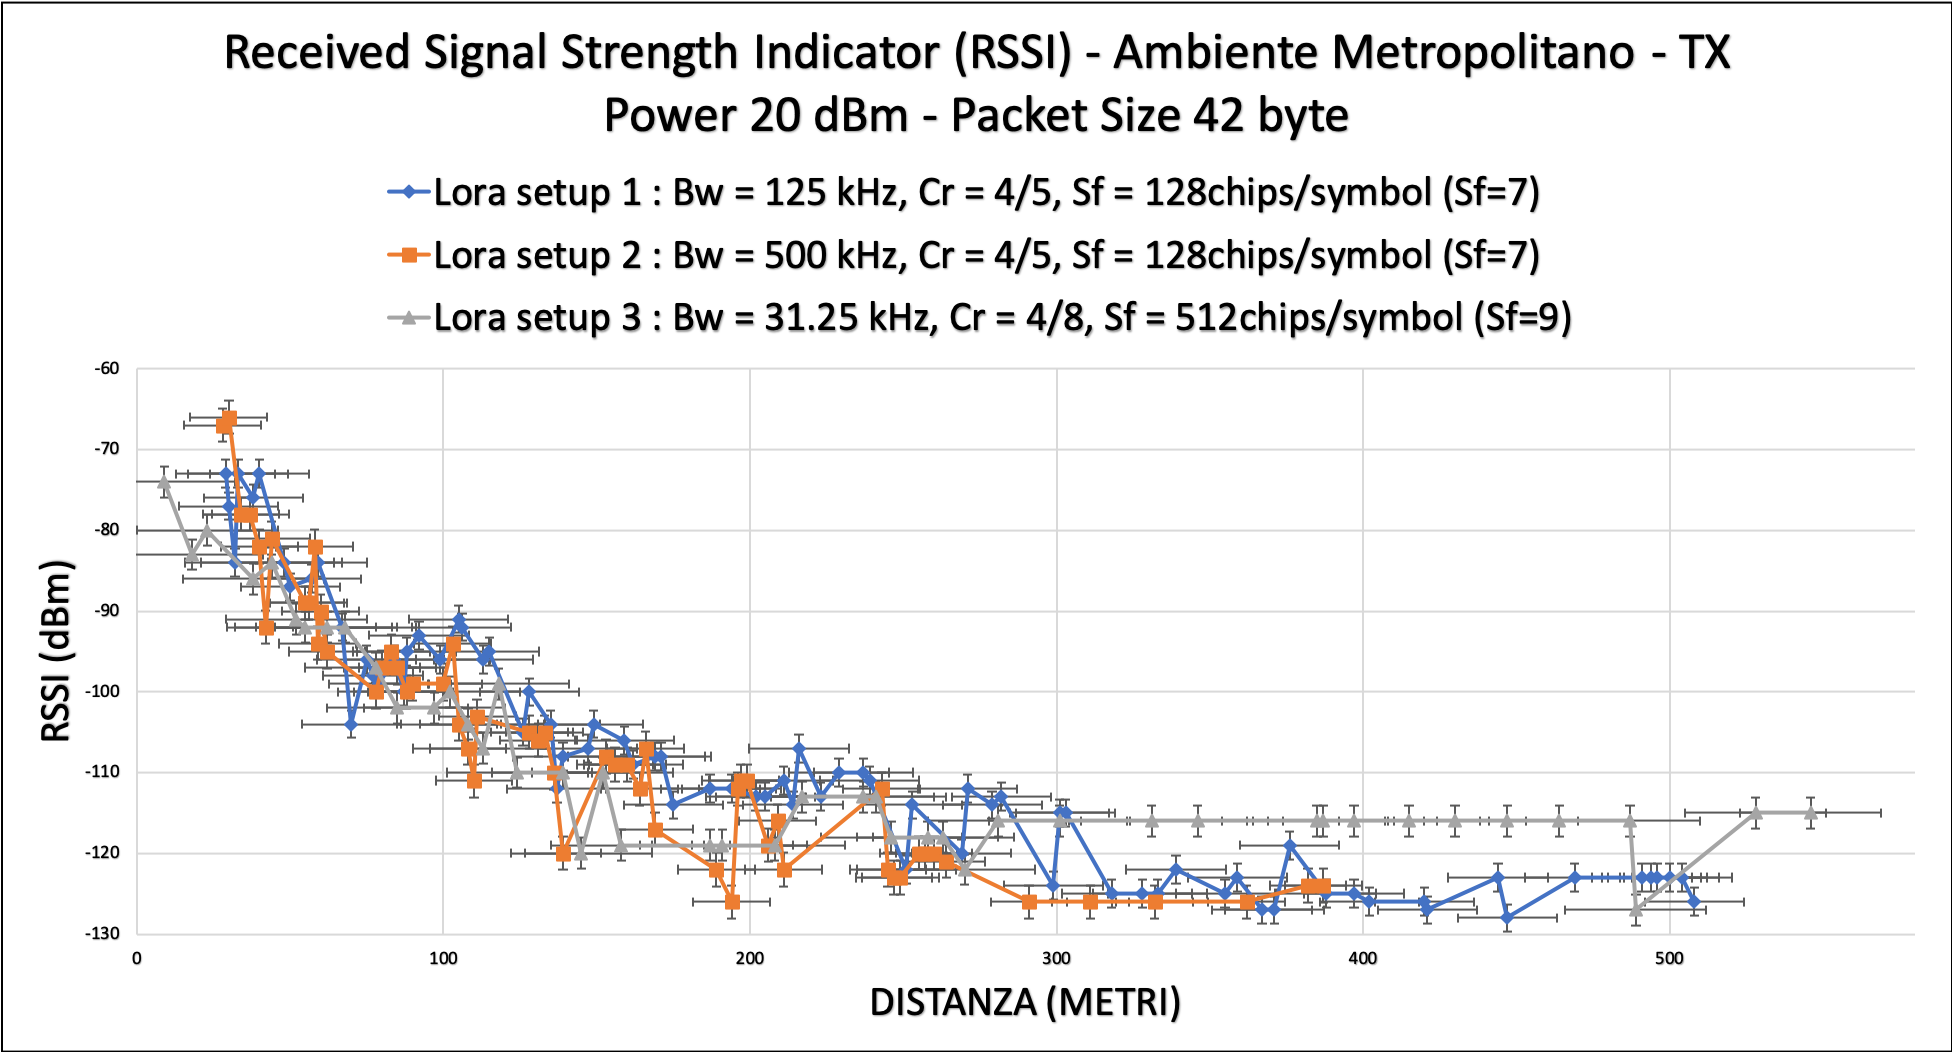
\includegraphics[width=\textwidth]{RSSI_confronto_AM-20dBm-42byte.png}
\caption[RSSI confronto Ambiente Metropolitano - 20 dBm - 42 byte]{RSSI confronto Ambiente Metropolitano - 20 dBm - 42 byte}\label{fig:prima}
\end{center}
\end{figure}

\begin{figure}[h]                      
\begin{center} 
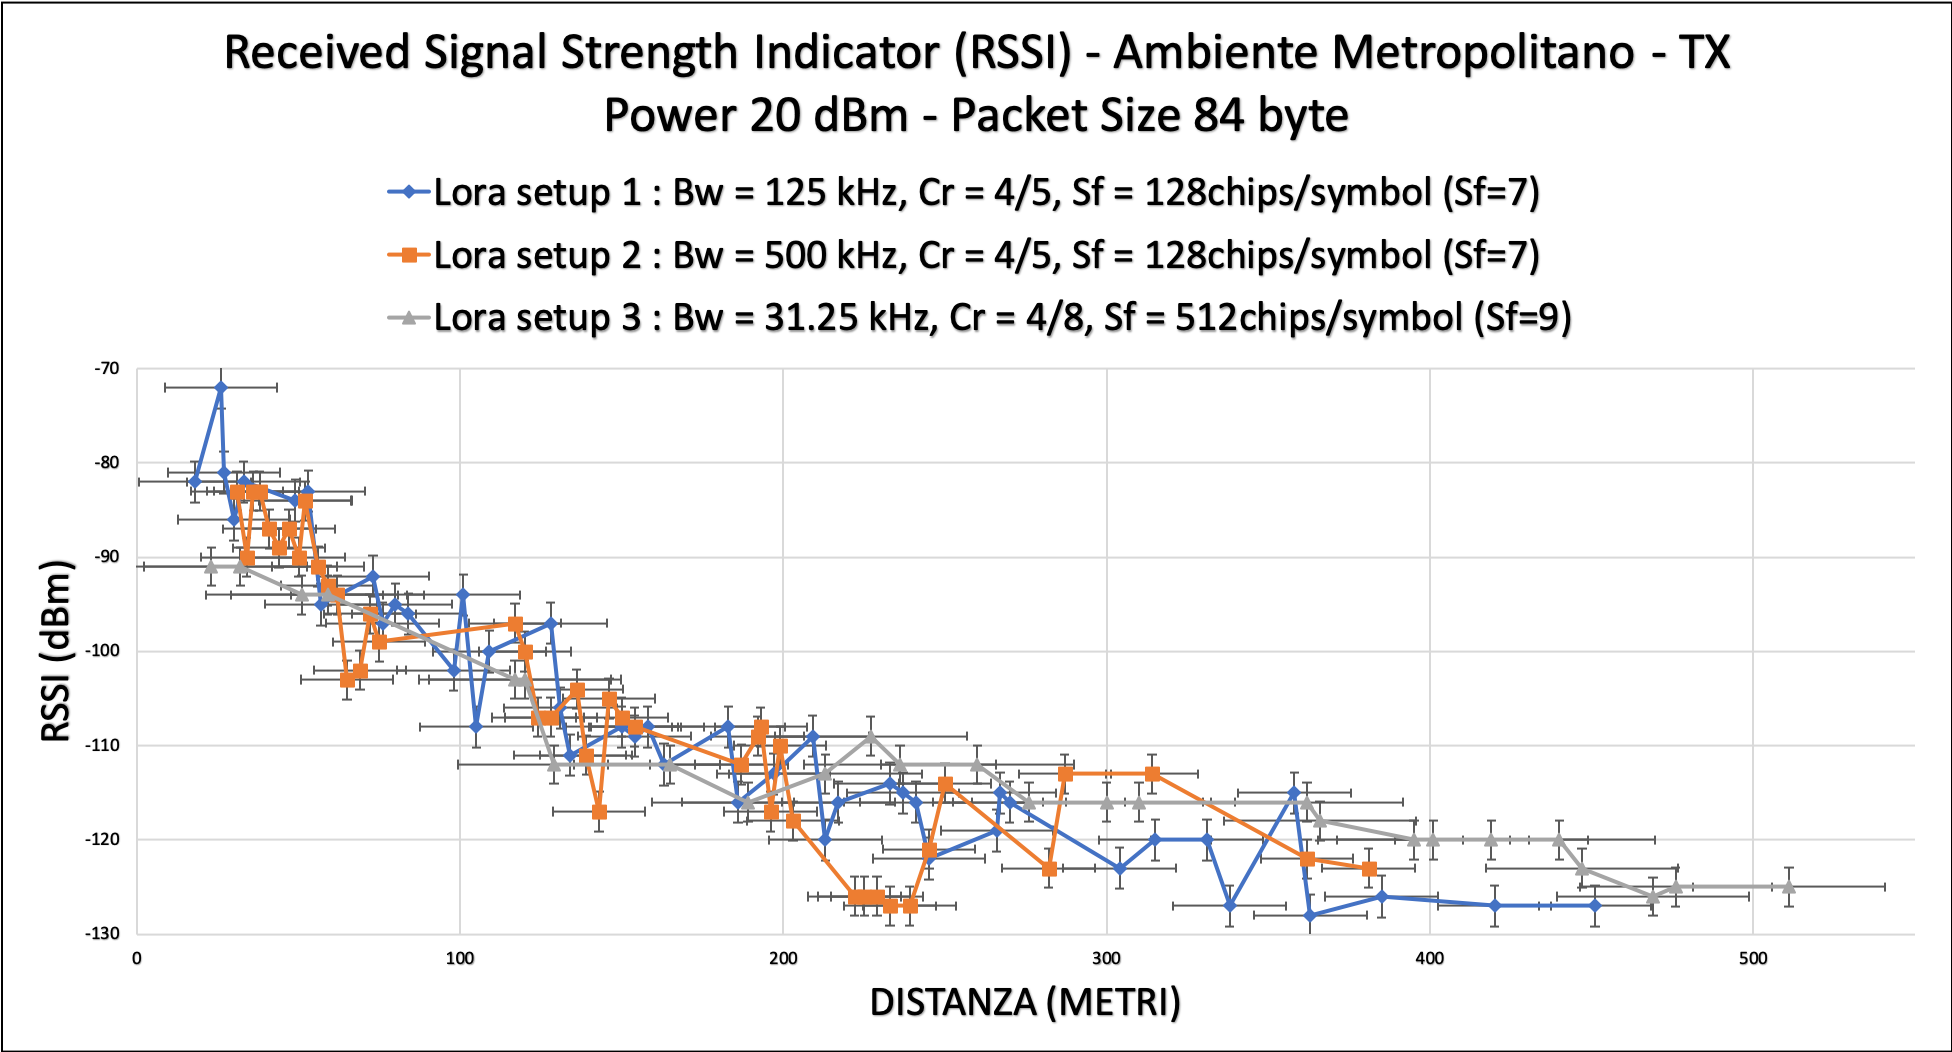
\includegraphics[width=\textwidth]{RSSI_confronto_AM-20dBm-84byte.png}
\caption[RSSI confronto Ambiente Metropolitano - 20 dBm - 84 byte]{RSSI confronto Ambiente Metropolitano - 20 dBm - 84 byte}\label{fig:prima}
\end{center}
\end{figure}

\begin{figure}[h]                      
\begin{center} 
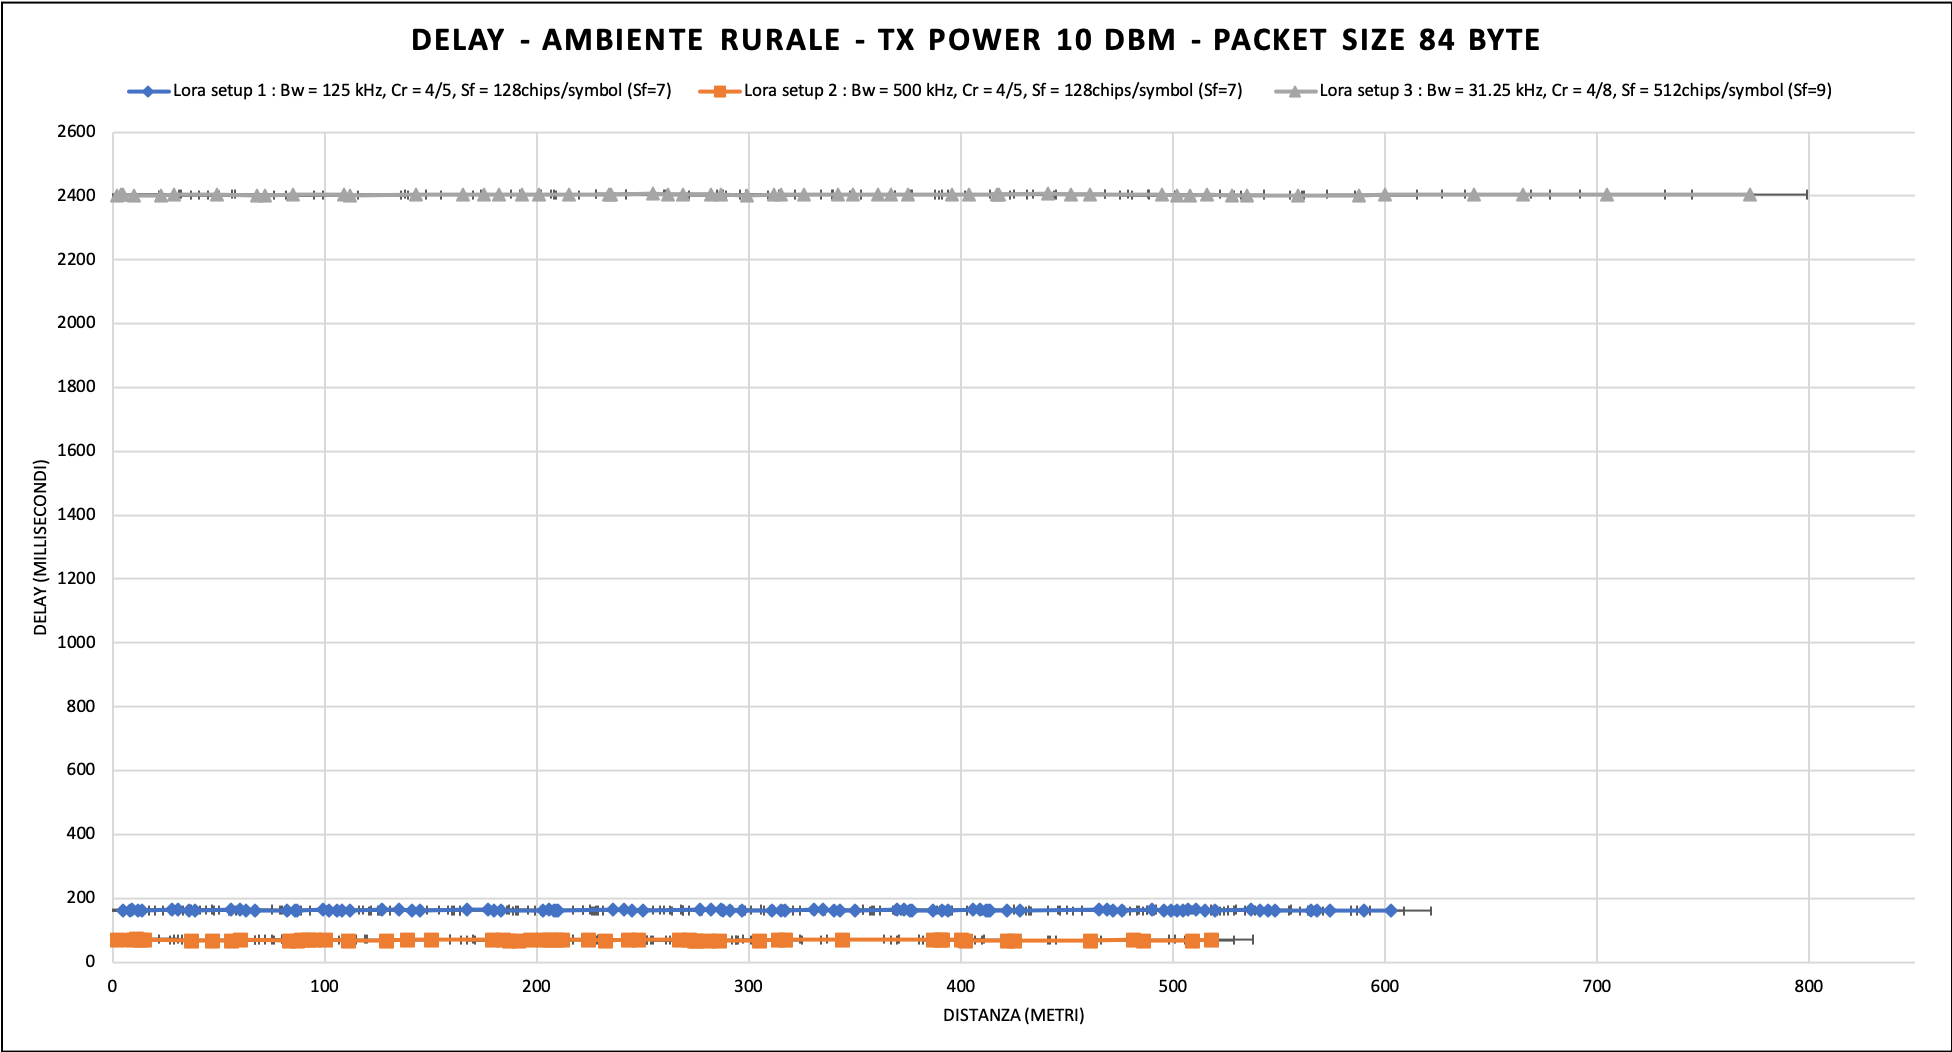
\includegraphics[width=\textwidth]{DELAY_confronto_AR_10dBm_84byte.png}
\caption[Delay confronto Ambiente Rurale - 10 dBm - 84 byte]{Delay confronto Ambiente Rurale - 10 dBm - 84 byte}\label{fig:prima}
\end{center}
\end{figure}

\begin{figure}[h]                      
\begin{center} 
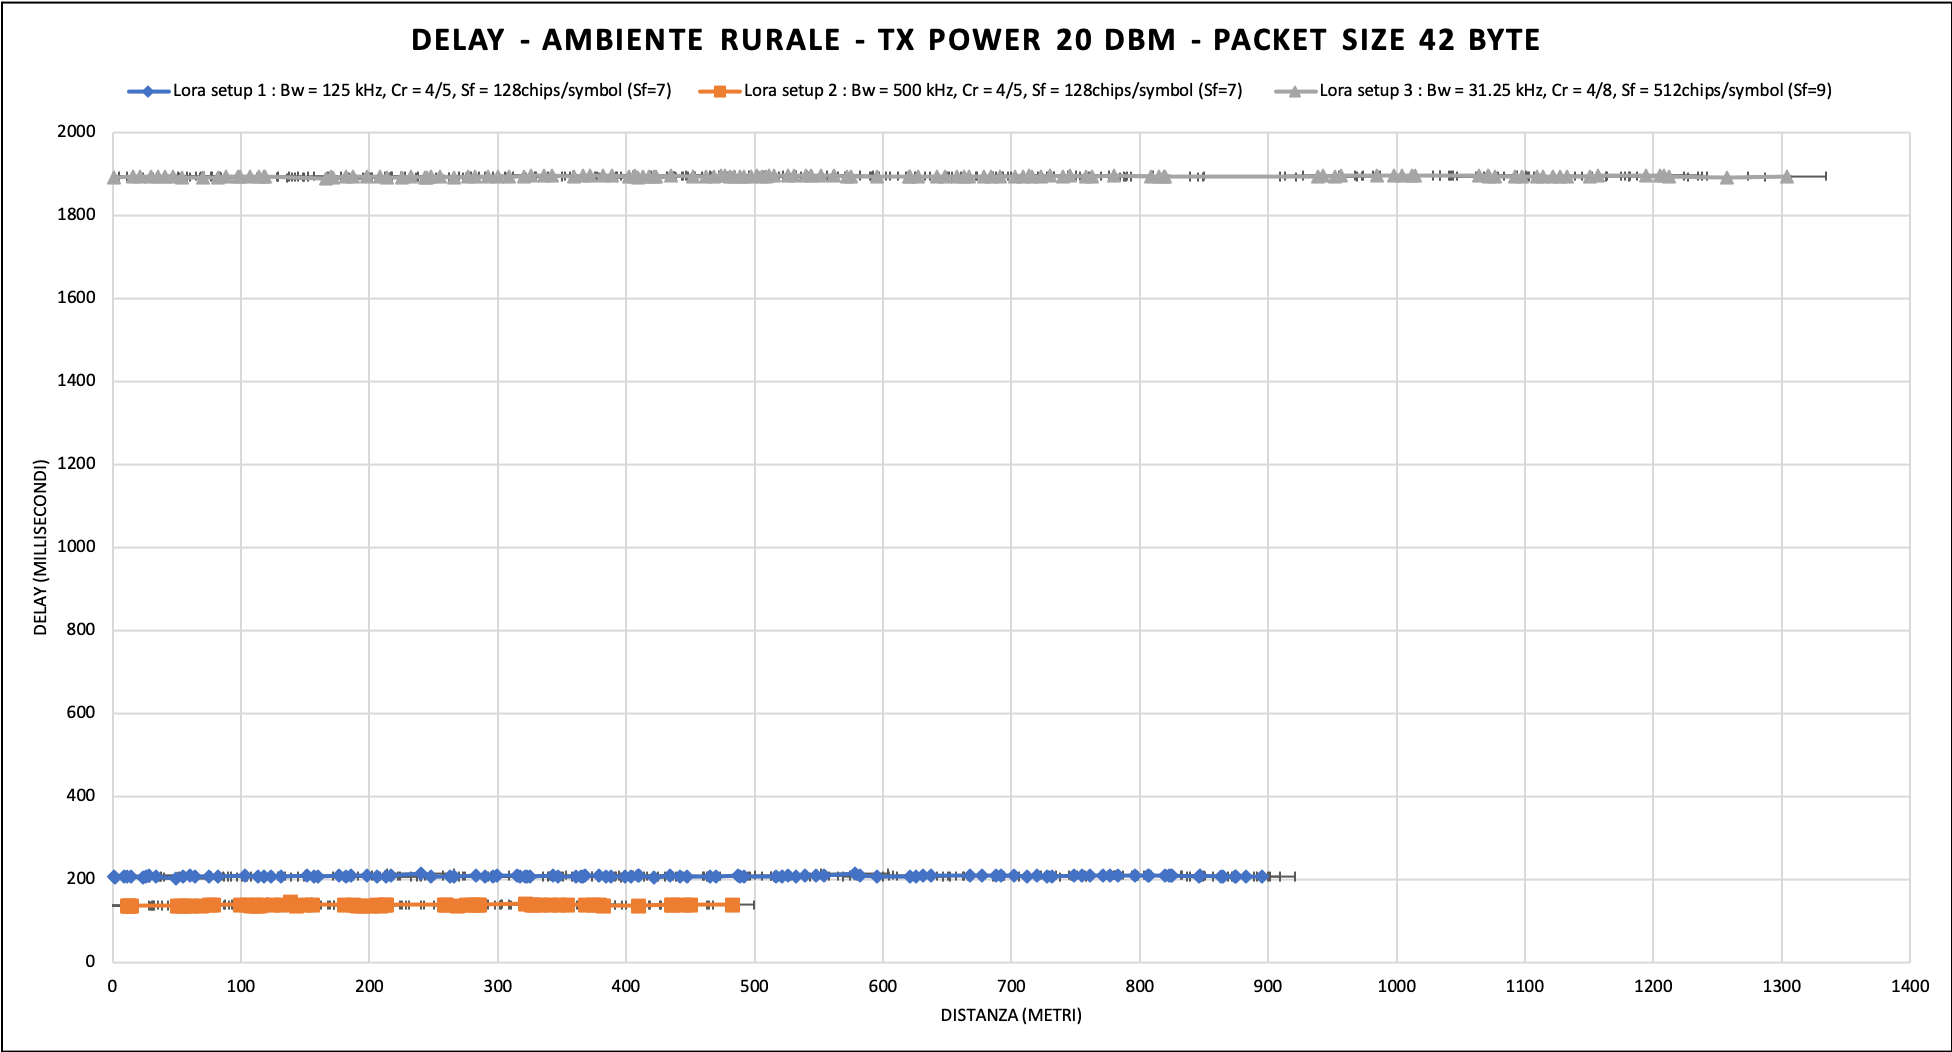
\includegraphics[width=\textwidth]{DELAY_confronto_AR_20dBm_42byte.png}
\caption[Delay confronto Ambiente Rurale - 20 dBm - 42 byte]{Delay confronto Ambiente Rurale - 20 dBm - 42 byte}\label{fig:prima}
\end{center}
\end{figure}

\begin{figure}[h]                      
\begin{center} 
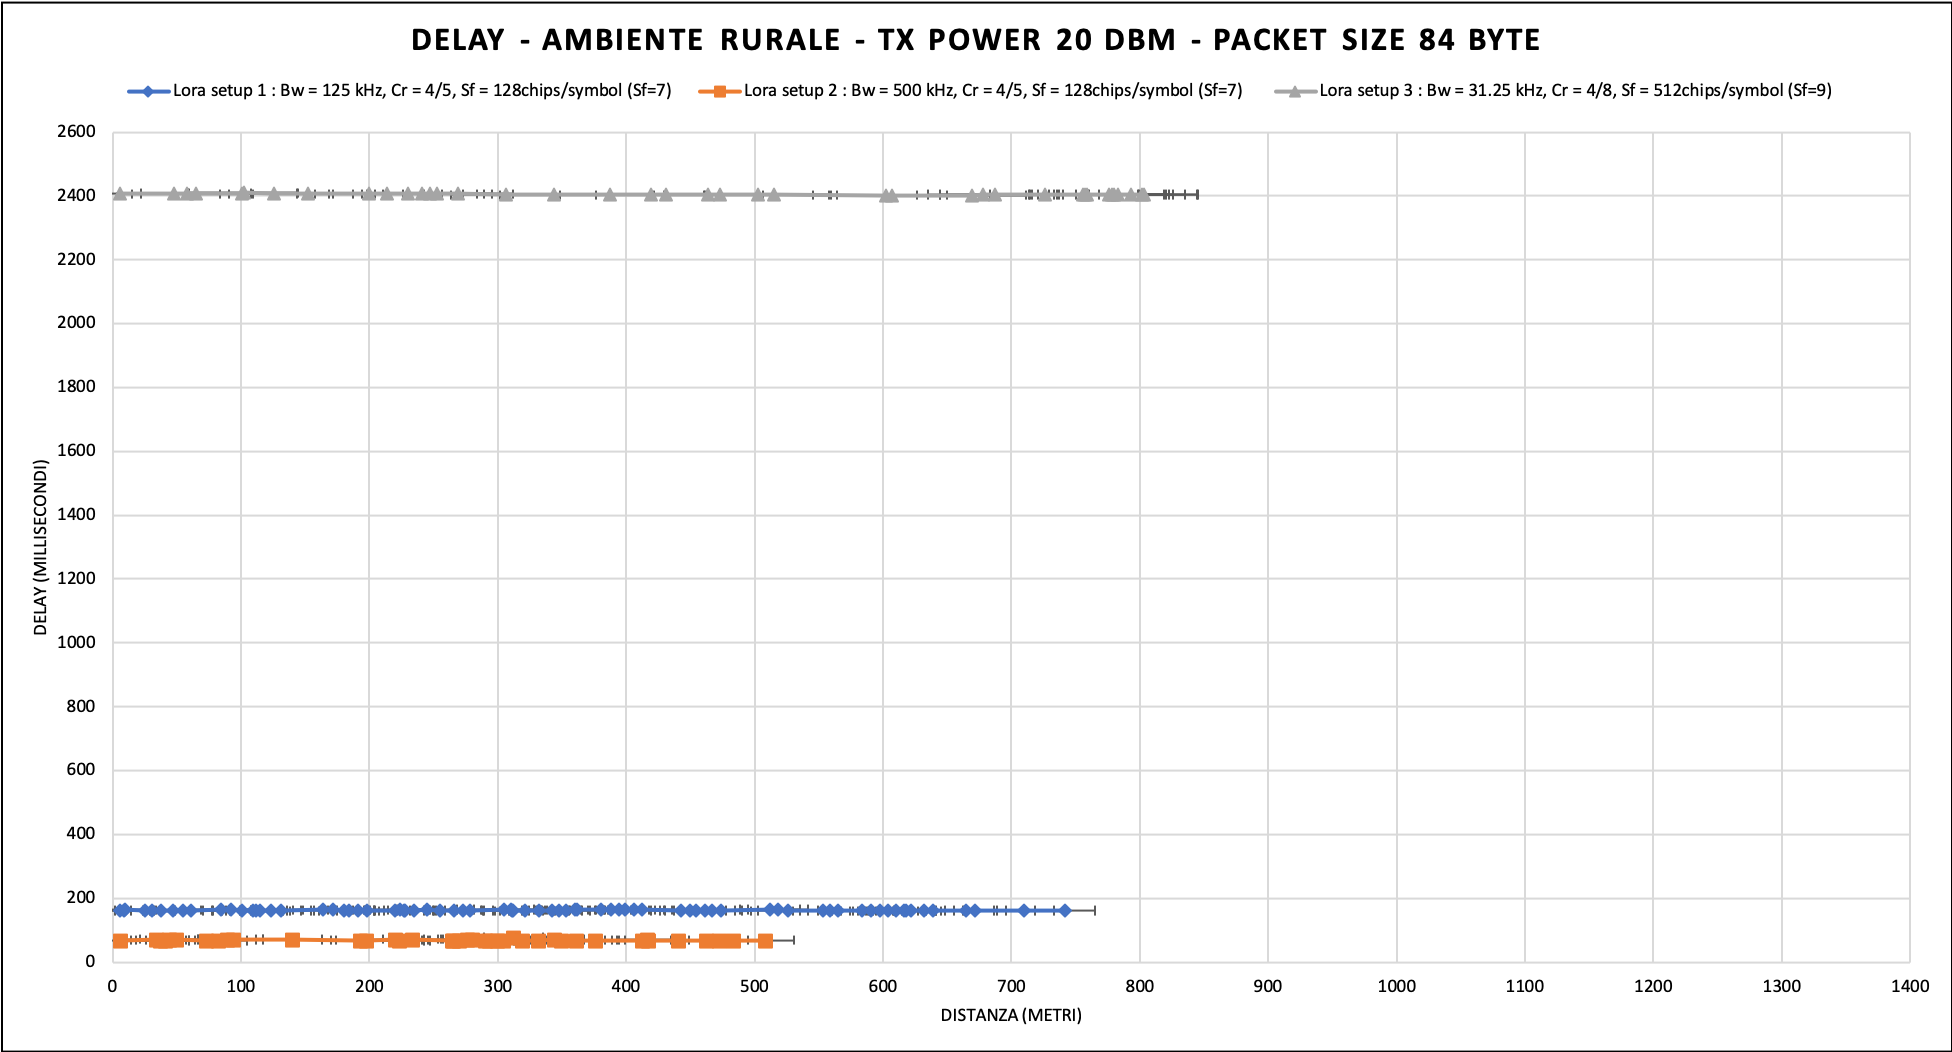
\includegraphics[width=\textwidth]{DELAY_confronto_AR_20dBm_84byte.png}
\caption[Delay confronto Ambiente Rurale - 20 dBm - 84 byte]{Delay confronto Ambiente Rurale - 20 dBm - 84 byte}\label{fig:prima}
\end{center}
\end{figure}

\begin{figure}[h]                      
\begin{center} 
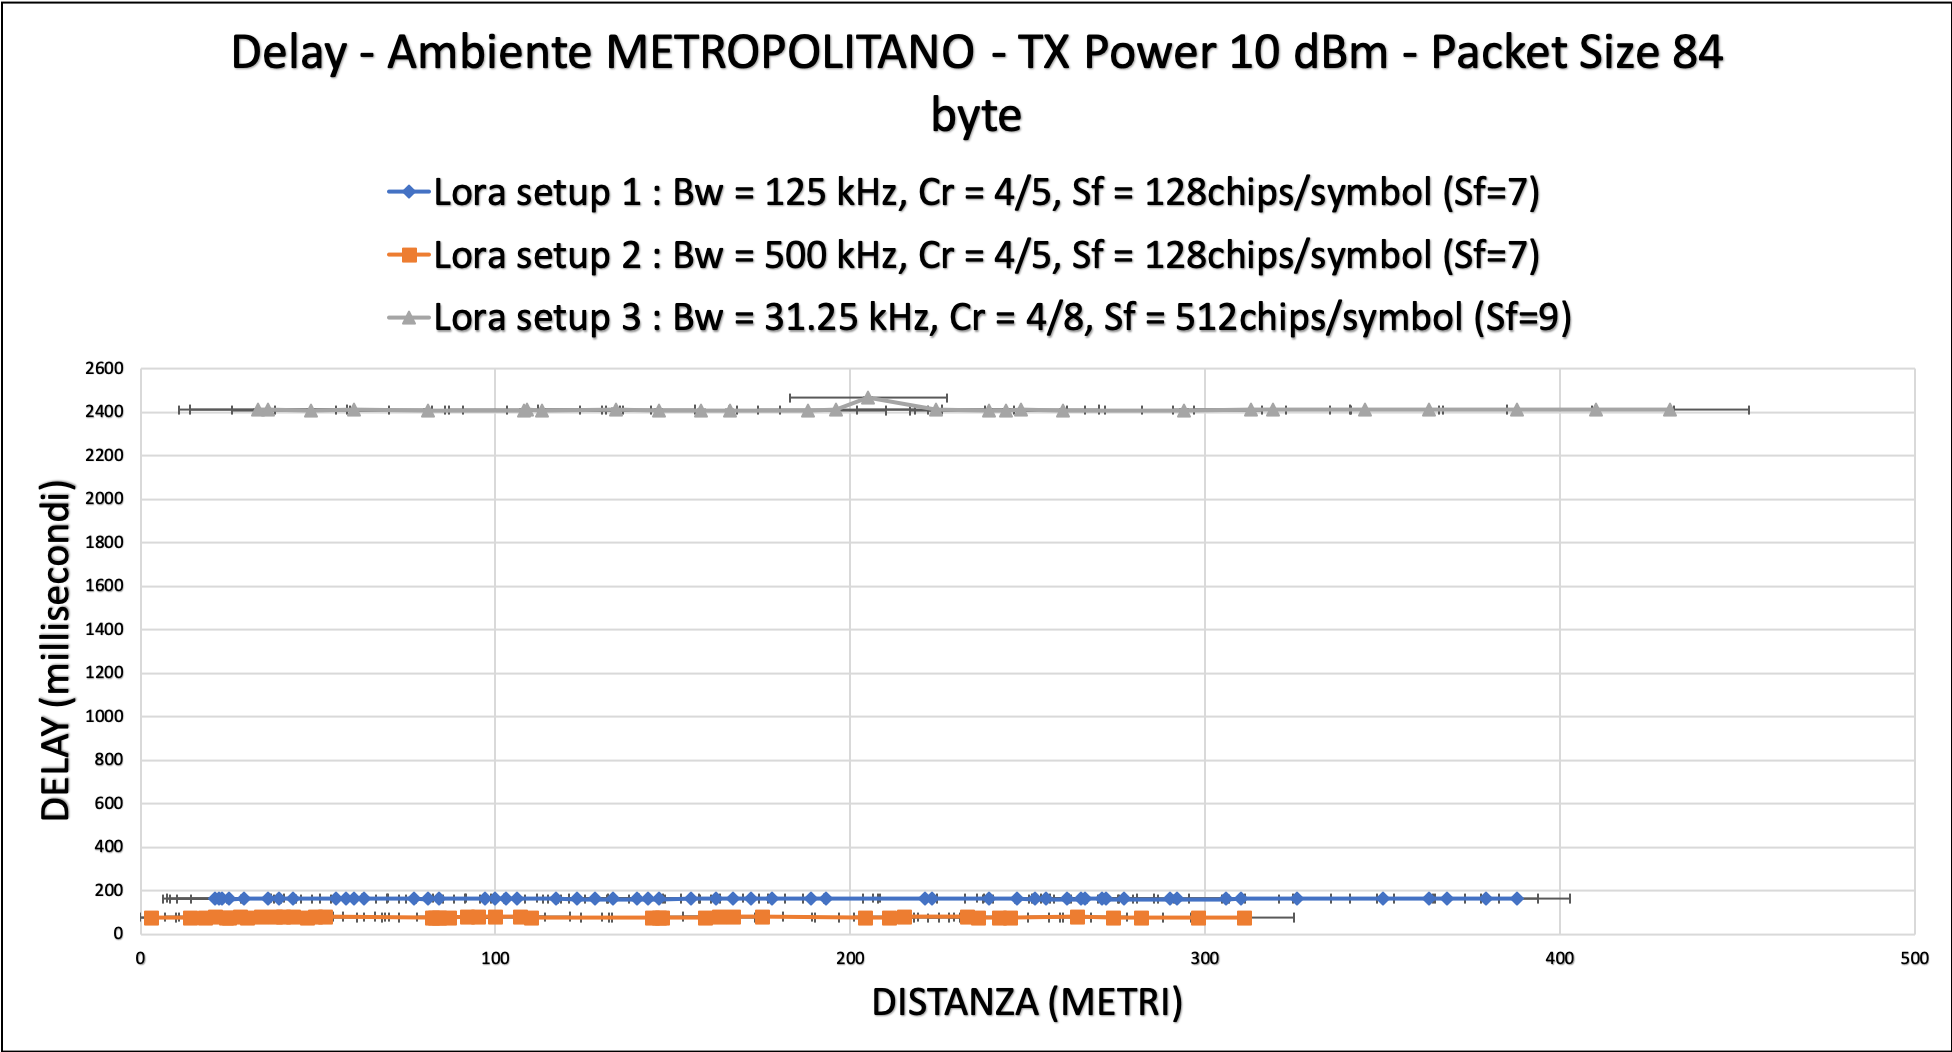
\includegraphics[width=\textwidth]{DELAY_confronto_AM_10dBm_84byte.png}
\caption[Delay confronto Ambiente Metropolitano - 10 dBm - 84 byte]{Delay confronto Ambiente Metropolitano - 10 dBm - 84 byte}\label{fig:prima}
\end{center}
\end{figure}

\begin{figure}[h]                      
\begin{center} 
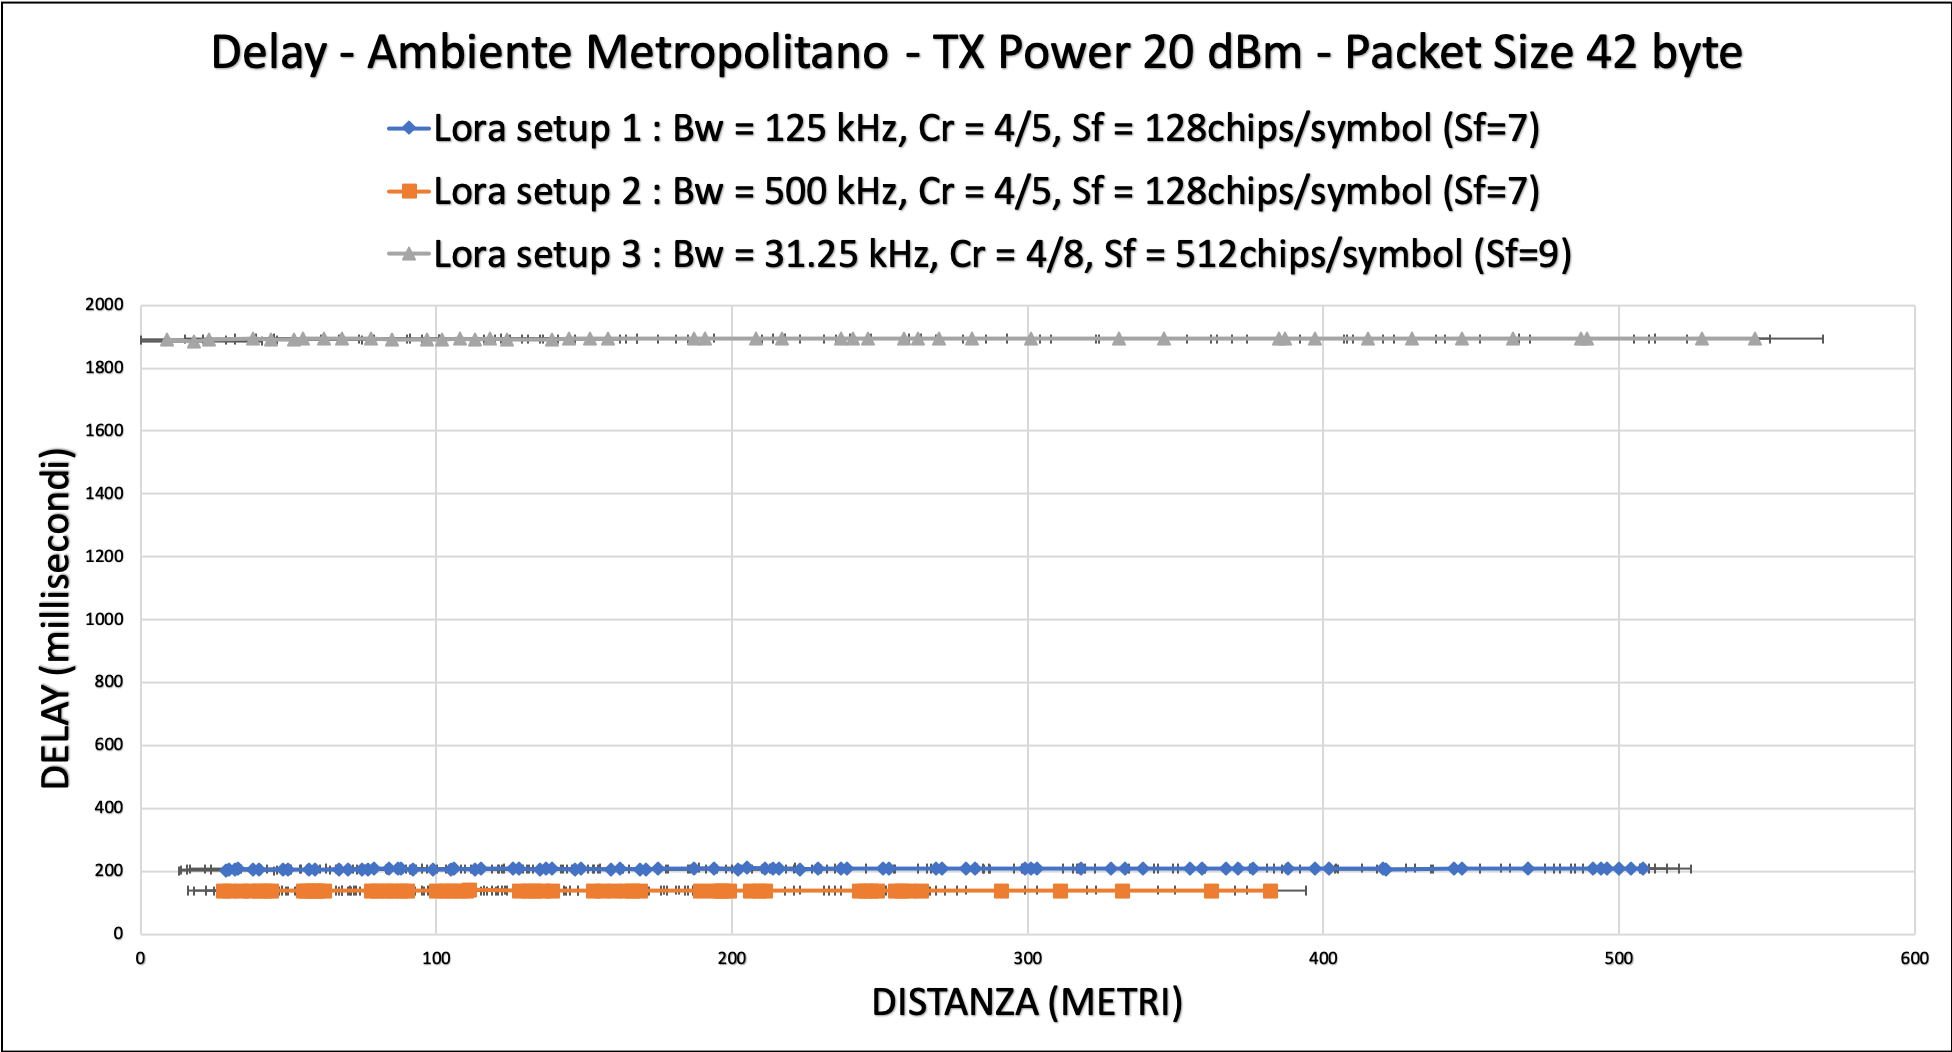
\includegraphics[width=\textwidth]{DELAY_confronto_AM_20dBm_42byte.png}
\caption[Delay confronto Ambiente Metropolitano - 20 dBm - 42 byte]{Delay confronto Ambiente Metropolitano - 20 dBm - 42 byte}\label{fig:prima}
\end{center}
\end{figure}

\begin{figure}[h]                      
\begin{center} 
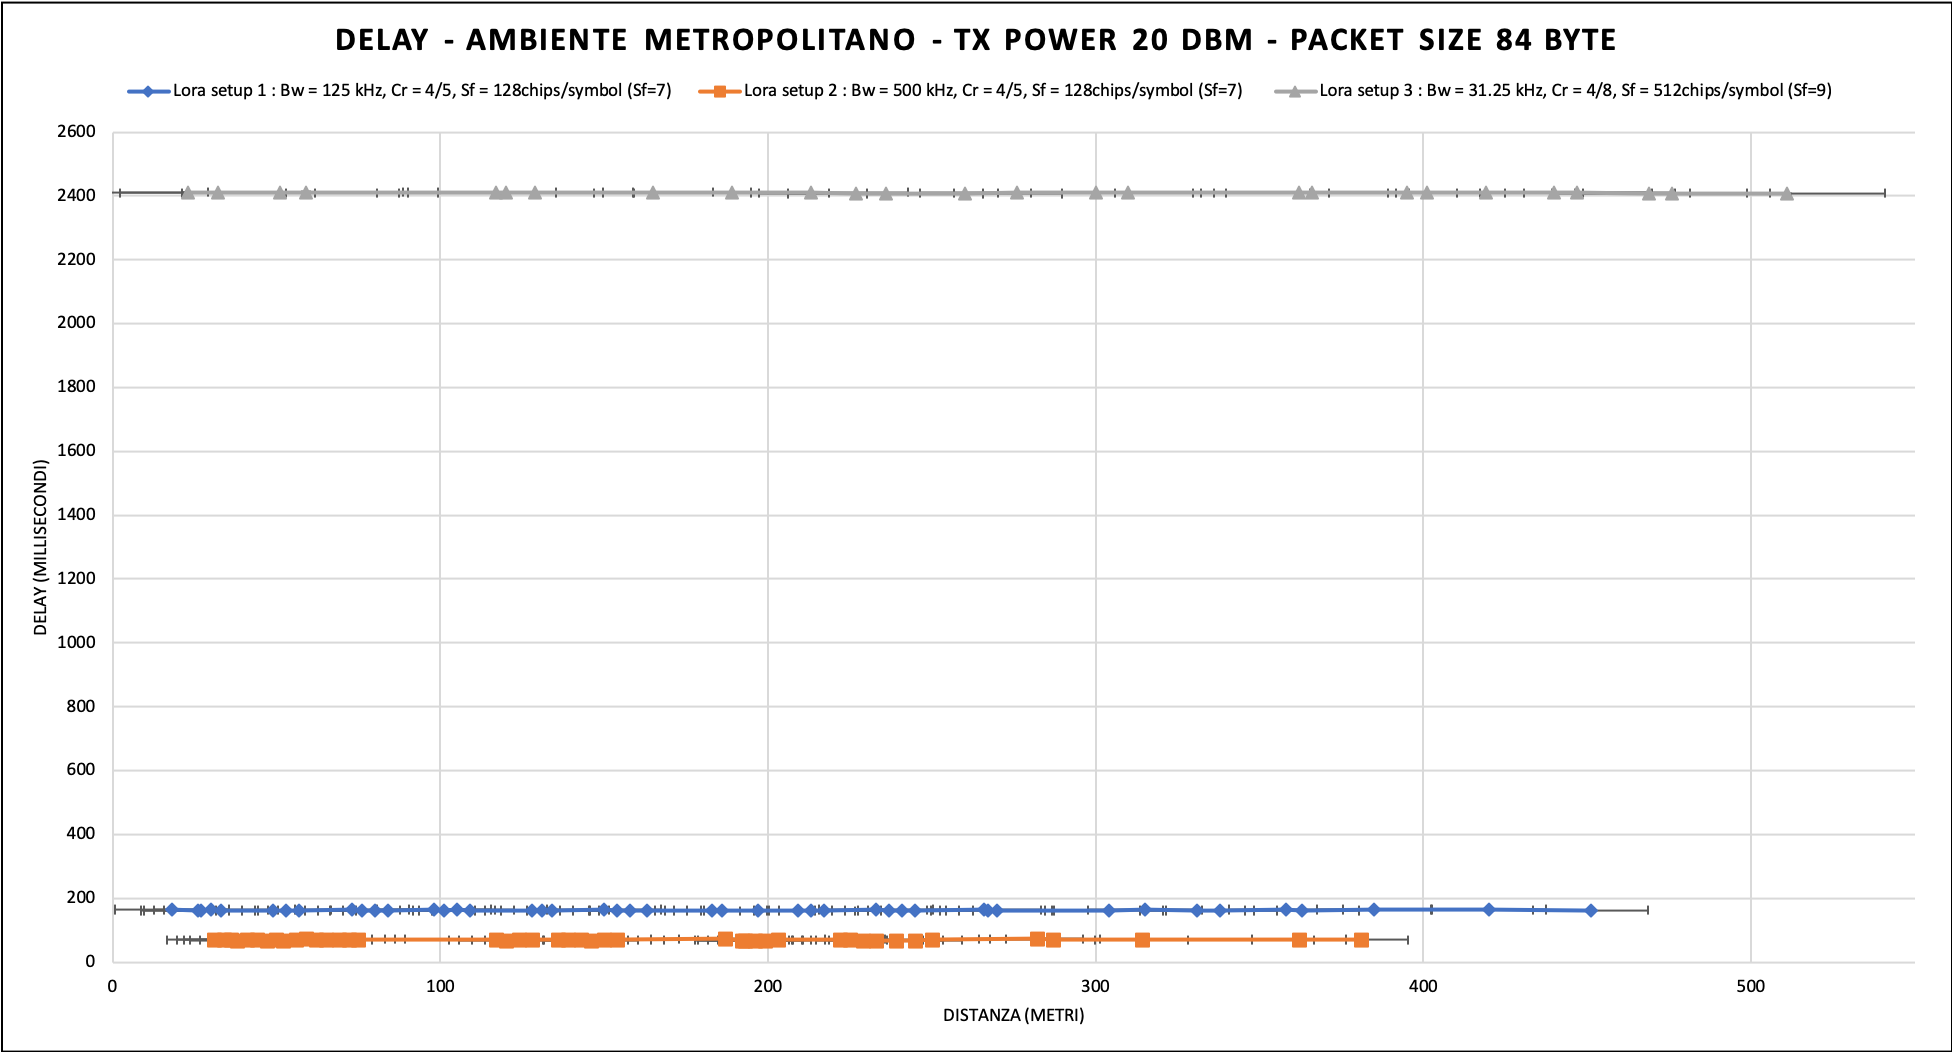
\includegraphics[width=\textwidth]{DELAY_confronto_AM_20dBm_84byte.png}
\caption[Delay confronto Ambiente Metropolitano - 20 dBm - 84 byte]{Delay confronto Ambiente Metropolitano - 20 dBm - 84 byte}\label{fig:prima}
\end{center}
\end{figure}





%\input{chapters/appendix}


\begin{thebibliography}{90}             %crea l'ambiente bibliografia
\rhead[\fancyplain{}{\bfseries \leftmark}]{\fancyplain{}{\bfseries
\thepage}}
%%%%%%%%%%%%%%%%%%%%%%%%%%%%%%%%%%%%%%%%%aggiunge la voce Bibliografia
                                        %   nell'indice
\addcontentsline{toc}{chapter}{Bibliografia}
%%%%%%%%%%%%%%%%%%%%%%%%%%%%%%%%%%%%%%%%%provare anche questo comando:
%%%%%%%%%%%\addcontentsline{toc}{chapter}{\numberline{}{Bibliografia}}
\bibitem{K1} Comparison of LoRaWAN Classes and their Power Consumption: Phui San Cheong, Johan Bergs, Chris Hawinkel, Jeroen Famaey IDLab, University of Antwerp imec, Antwerp, Belgium Nokia Bell Labs, Antwerp, Belgium


\bibitem{K2} Low Power Wide Area Networks: An Overview : Usman Raza, Parag Kulkarni, and Mahesh Sooriyabandara
\bibitem{K3} ``Nb-iot : enabling new business opportunities'' Hawei Technologies
Co., Tech. Rep., 2015. [Online]. Available: http://www.huawei.com/
minisite/4-5g/img/NB-IOT.pdf
\bibitem{K4} Sigfox's ecosystem delivers the worlds first ultra-low cost
modules to fuel the internet of things mass market
deployment. [Online]. Available: https://www.sigfox.com/en/press/
sigfox-s-ecosystem-delivers-world-s-first-ultra-low-cost-modules-to-fuel-internet-of-things

\bibitem{K5} QoS Metrics Measurement in Long Range IoT Networks: Andrey Dvornikov, Pavel Abramov, Sergey Efremov, Leonid Voskov,National Research University Higher School of Economics (HSE) - Moscow, Russia 

\bibitem{K6} Ingenu : https://www.leverege.com/blogpost/rpma-technical-drill-down-ingenus-lpwan-technology

\bibitem{K7} Performance Evaluation of IEEE 802.15.4k Priority Channel Access with DSSS PHY : Berhane G. Gebremedhin, Jussi Haapola and Jari Iinatti Center for Wireless Communications, University of Oulu P.O.Box 4500,FI-90014 Oulu, Finland.

\bibitem{K8} Design and Implementation of LPWA-Based Air Quality Monitoring System: KAN ZHENG, (Senior Member, IEEE), SHAOHANG ZHAO , ZHE YANG, XIONG XIONG, AND WEI XIANG , (Senior Member, IEEE).

\bibitem{K9} Feasibility Study of IEEE 802.11ah Radio Technology for loT and M2M use Cases : Berhane G. Gebremedhin, Jussi Haapola and Jari Iinatti Center for Wireless Communications, University of Oulu P.O.Box 4500,FI-90014 Oulu, Finland

\bibitem{K10} Weightless. [Online]. Available: http://www.weightless.org/

\bibitem{K11} ``Do lora low-power wide-area networks scale?'' in Proceedings of the 19th
ACM International Conference on Modeling, Analysis and Simulation
of Wireless and Mobile System 

\bibitem{K12} ``Low power wide area network analysis: Can lora scale?'' : O. Georgiou and U. Raza


\bibitem{K13} ``Goodbye, aloha'' : ANDRES LAYA, (Student Member, IEEE), CHARALAMPOS KALALAS, (Student Member, IEEE), FRANCISCO VAZQUEZ-GALLEGO, (Senior Member, IEEE), LUIS ALONSO, (Senior Member, IEEE), AND JESUS ALONSO-ZARATE, (Senior Member, IEEE)

\bibitem{K14} ``Software defined Radio'' :  https://patents.google.com/patent/US20040242261A1/en

\bibitem{K15} Interference measurements in the european 868 mhz ism band with focus on lora and sigfox: Mads Lauridsen, Benny Vejlgaar, Istvan Z. Kovacs, Huan Nguyen, Preben Mogensen, Dept. of Electronic Systems, Aalborg University, Denmark Nokia Bell Labs, Aalborg

\bibitem{K16} Role Of Middleware For Internet Of Things: A Study [ONLINE] : 
https://www.researchgate.net/publication/266287969\_Role\_Of\_Middleware\_For\_Internet\_Of\_Things\_A\_Study
				
\bibitem{K17} Wireless Position Location: Fundamentals, Implementation Strategies, and Sources of Error: K. J. Krizman, T. E. Biedka, and S. Rappaport,

\bibitem{K18} Demystifying low-power wide-area communications for city iot applications : 
S. Kartakis, B. D. Choudhary, A. D. Gluhak, L. Lambrinos, and J. A. McCann,

\bibitem{K19} The analysis of 6LowPAN technology : Xin Ma, Wei Luo. The Key Laboratory of Network Control Technology and Intelligent Instrument Chongqing University of Posts and Telecommunications Chongqing 400065, China

\bibitem{K20}On the Application of LoRa LPWAN Technology in Sailing Monitoring System : 	
Lingling Li, Jiuchun Ren, Qian Zhu - Department of Communication Science and Engineering
Fudan University, Shanghai, China

\bibitem{K21} Semtech's datasheets : https://www.semtech.com/uploads/documents/sx1272.pdf

\bibitem{K22} Comparison of LoRaWAN Classes and their Power Consumption: Phui San Cheong, Johan Bergs, Chris Hawinkel, Jeroen Famaey IDLab, University of Antwerp imec, Antwerp, Belgium Nokia Bell Labs, Antwerp, Belgium

\bibitem{K23} Understanding the Limits of LoRaWAN : Ferran Adelantado, Xavier Vilajosana, Pere Tuset-Peiro, Borja Martinez, Joan Meli\`a-Seguí, Thomas Watteyne.

\bibitem{K24} Exploring the Security Vulnerabilities of LoRa :  Emekcan Aras, Gowri Sankar Ramachandran, Piers Lawrence and Danny Hughes - iMinds-DistriNet, KU Leuven, 3001 Leuven, Belgium.

\bibitem{K25} \hyperref[industry4]{https://www.researchgate.net/publication/322505680\_What\_Drives\_the\_Implementation\_of\_Industry\_40\_The\_Role\_of\_Opportunities\_and\_Challenges\_in\_the\_Context\_of\_Sustainability}

\bibitem{K26} Past, present and future of Industry 4.0. A systematic literature review and research agenda proposal: Yongxin Liao, Fernando Deschamps, Eduardo de Freitas Rocha Loures, Luiz Felipe Pierin Ramos
\hyperref[industry4]{https://www.tandfonline.com/doi/full/10.1080/00207543.2017.1308576}

\bibitem{K27} Sistemi informativi aziendali e agricoltura di precisione: Fabrizio Mazzetto, Michael Riedel, Pasqualina Sacco - Agricoltura di precisione - Edagricole  

\bibitem{K28} On the Application of LoRa LPWAN Technology in Sailing Monitoring System: Lingling Li, Jiuchun Ren, Qian Zhu - Department of Communication Science and Engineering
Fudan University, Shanghai, China

\end{thebibliography}
\end{document}
